\chapter{Θεωρητικό Υπόβαθρο}

Στο παρόν κεφάλαιο θα οικοδομήσουμε την απαραίτητη γνώση στην οποία βασίζεται η έρευνα των επόμενων ενοτήτων. Αρχικά, θα παρουσιαστούν συνοπτικά τα τεχνητά νευρωνικά δίκτυα \footnote{Από εδώ και στο εξής, με τον όρο \textquote{νευρωνικά δίκτυα} θα αναφερόμαστε στα \textquote{τεχνητά νευρωνικά δίκτυα}.} υπό μια μαθηματική σκοπιά. Έπειτα, θα αναλυθούν τα \hyperlink{_capsule_networks}{νευρωνικά δίκτυα με κάψουλες} (\hyperlink{_capsule_networks}{\en{capsule networks}}) τα οποία και αποτελούν το κύριο θέμα της εργασίας. Τέλος, θα γίνει αναφορά σε νέες τεχνικές και αλγορίθμους που χρησιμοποιήθηκαν στο παρόν έργο ώστε η μετέπειτα εισαγωγή των μεθόδων μας για την εξέλιξη των νευρωνικών δικτύων με κάψουλες να είναι περισσότερο ομαλή και κατανοητή.

\section{Τεχνητά Νευρωνικά Δίκτυα}
Τα σημερινά τεχνητά νευρωνικά δίκτυα, όπως είναι αναμενόμενο, απέχουν σημαντικά από το πρώτο μοντέλο των \en{Warren McCulloch} και \en{Walter Pitts} \cite{mcculloch1943logical} που συζητήσαμε στην ενότητα \ref{sec:historic_note}. Με την ωρίμανση της τεχνολογίας, αυτή ανεξαρτητοποιήθηκε από την \hyperlink{_computational_neuroscience}{(υπολογιστική) νευροεπιστήμη} και εντάχθηκε στην Τεχνητή Νοημοσύνη υπό μια ιεραρχική δομή. Κρίνεται λοιπόν σκόπιμο να παρουσιάσουμε αυτήν την ιεραρχική δομή οργάνωσης της Τεχνητής Νοημοσύνης και μετέπειτα να αναφερθούμε στα επιμέρους στοιχεία της.
\par

\begin{figure}[h]
    \centering
    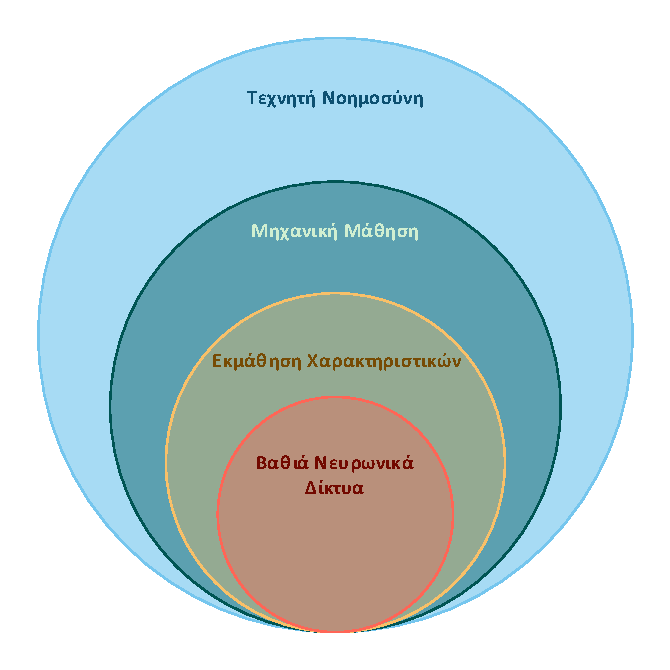
\includegraphics[width=0.7\textwidth]{images/chapter theoritical background/venn ai diagram thesis in greek new 2.pdf}
    \caption{Διάγραμμα \en{Venn} όπου απεικονίζει τη θέση των νευρωνικών δικτύων στην οργάνωση της τεχνητής νοημοσύνης. \textit{Παράχθηκε από το \href{https://www.microsoft.com/en-gb/microsoft-365/visio/flowchart-software/}{\en{Microsoft Visio\texttrademark}.}} }
    \label{fig:_venn_ai}
\end{figure}

Όπως βλέπουμε στο σχήμα \ref{fig:_venn_ai} τα νευρωνικά δίκτυα πολλών επιπέδων (βαθιά νευρωνικά δίκτυα) είναι ένα μέρος του κλάδου της εκμάθησης χαρακτηριστικών (\en{feature learning} ή \en{representation learning}) που είναι ένα μέρος της μηχανικής μάθησης η οποία με τη σειρά της ανήκει στο ευρύτερο επιστημονικό πεδίο της τεχνητής νοημοσύνης. Φυσικά, η τεχνητή νοημοσύνη περιλαμβάνει αρκετούς άλλους κλάδους εκτός από αυτόν της μηχανικής μάθησης\footnote{Βέβαια, ο κλάδος της μηχανικής μάθησης είναι σήμερα ο γρηγορότερα αναπτυσσόμενος.}. Μια χρήσιμη παρατήρηση είναι ότι οι σχέσεις υποσυνόλου συμπίπτουν με τη χρονική αλληλουχία ανάπτυξης του κάθε κλάδου. Δηλαδή, κάθε υποσύνολο αναπτύχθηκε ταυτόχρονα ή αργότερα από το οποιοδήποτε υπερσύνολό του.
\par
Στη συνέχεια, θα γίνει λόγος για τα στοιχεία εκείνα που περιλαμβάνουν την τεχνολογία των βαθιών νευρωνικών δικτύων προκειμένου ο αναγνώστης να αποκτήσει μια εποπτικότερη εικόνα.

\subsection{Μηχανική Μάθηση}


Όπως προδίδει ο όρος, σε αδρές γραμμές τα συστήματα μηχανικής μάθησης έχουν τη δυνατότητα να μαθαίνουν μια εργασία χωρίς να έχουν προγραμματιστεί με ρητές εντολές για τη συγκεκριμένη εργασία αυτή\footnote{Η δυνατότητα αυτή είναι πολύ σημαντική αφού, όπως διαπιστώσαμε στην ενότητα \ref{sec:historic_note} όταν έγινε λόγος για τα έμπειρα συστήματα, για πολλές εργασίες είναι πρακτικός αδύνατο να περιγραφούν ρητά και ντετερμινιστικά οι λύσεις τους.}. Ίσως, ο πιο πλήρης ορισμός δίνεται από τον \en{Tom M. Mitchell} \cite{mitchell1997machine} σύμφωνα με τον οποίο, ένα υπολογιστικό πρόγραμμα λέγεται ότι μαθαίνει από μια εμπειρία \en{E}, ως προς ένα σύνολο εργασιών \en{T} και ένα μέτρο απόδοσης \en{P}, εάν η απόδοσή του σε εργασίες του \en{T}, όπως αυτή μετριέται από το \en{P}, βελτιώνεται με την \en{E}. \footnote{Ο ορισμός αυτός εξηγεί γιατί για παράδειγμα η λήψη μιας ιστοσελίδας της βικιπέδιας και η αποθήκευσή της τοπικά στον υπολογιστή δεν αποτελεί μηχανική μάθηση. Όπως προκύπτει, η \textquote{γνώση} αυτή δεν καθιστά καλύτερο τον υπολογιστή σε κάποια εργασία\cite{geron2019hands}.}
\par

Σύμφωνα με τον ανωτέρω ορισμό διακρίνουμε τρία βασικά συστατικά ενός συστήματος μηχανικής μάθησης. Αυτά είναι τα παρακάτω:
\begin{description}
\item [Εργασία - \en{T}] Είναι το πρόβλημα το οποίο επιθυμούμε να λύσουμε.
\item [Μέτρο Απόδοσης - \en{P}] Αποτελεί μια μετρική του στόχου ως ένδειξη ποιότητας της λύσης μας. Από μαθηματική σκοπιά, είναι αυτό που ο αλγόριθμος μάθησης βελτιστοποιεί.
\item [Εμπειρία - \en{E}] Πρόκειται για τα δεδομένα εισόδου που λαμβάνει το σύστημα υπό τη μορφή παραδειγμάτων ή ως ερεθίσματα ανάδρασης από το περιβάλλον. Όπως θα δούμε στη συνέχεια, ο τρόπος απόκτησης αυτών των δεδομένων αλλά και η φύση τους καθορίζει το είδος της μάθησης.
\end{description}

\subsubsection{Βασικά Είδη Συστημάτων Μηχανικής Μάθησης}
\label{sec:_ML_varieties}
Τα είδη των συστημάτων μηχανικής μάθησης μπορούν να ταξινομηθούν ανάλογα με το:
\begin{itemize}
    \item \emph{Αν εκπαιδεύονται με ανθρώπινη επίβλεψη.}\\
    Ανάλογα με αυτό το κριτήριο έχουμε τις εξής βασικές κατηγορίες: επιβλεπόμενη (\en{supervised}), μη-επιβλεπόμενη (\en{un-supervised}) και ενισχυτική μάθηση (\en{reinforcement learning}).
    \item \emph{Αν μαθαίνουν σταδιακά (\en{incrementally}) και \textquote{στον αέρα} (\en{on the fly}).}\\
    Σε αυτήν την περίπτωση χωρίζουμε τα συστήματα μηχανικής μάθησης σε αυτά που πραγματοποιούν μάθηση σε ζωντανό χρόνο (\en{online learning}) και σε αυτά που μαθαίνουν κατά δέσμες (\en{batch learning}).
    \item \emph{Αν κατασκευάζουν μοντέλα προσαρμοσμένα στα δεδομένα.}\\ 
    Με αυτό το κριτήριο χωρίζονται σε συστήματα βασισμένα σε μοντέλο (\en{model-based}) ή σε συστήματα βασισμένα σε παραδείγματα (\en{instance-based}). \cite{geron2019hands}
\end{itemize}

Προφανώς, κάθε δυνατός συνδυασμός των παραπάνω κριτηρίων είναι αποδεκτός, οδηγώντας έτσι στην ταξινόμηση των συστημάτων μηχανικής μάθησης σε μια πληθώρα από διαφορετικές κατηγορίες. Κρίνεται χρήσιμο, να αναφέρουμε σε όλη την έκταση του έργου τις κατηγορίες στις οποίες ανήκει το κάθε σύστημα που παρουσιάζουμε. Για αυτόν τον λόγο, παροτρύνουμε τον αναγνώστη που δεν είναι εξοικειωμένος με τους ανωτέρω όρους να διαβάσει τους αντίστοιχους ορισμούς στο παράρτημα \ref{chap:definitions}. 

\subsection{Εκμάθηση Χαρακτηριστικών}
\label{sec:_feature_extraction}
Η ανάπτυξη των πρώτων συστημάτων μηχανικής μάθησης απεμπόλησε την ανάγκη των ευφυών εφαρμογών για σχολαστική και ρητή (\en{hard-coded}) αναπαράσταση του χώρου του προβλήματος (π.χ. με την χρήση προτασιακής λογικής). Με τα νέα συστήματα, η γνώση για το πρόβλημα μαθαίνονταν αυτοματοποιημένα μέσω αλγορίθμων μάθησης από το σύνολο δεδομένων εκπαίδευσης. Με άλλα λόγια, τα αλγοριθμικά κατασκευάσματα μάθαιναν να αντιστοιχίζουν με αυτοματοποιημένο τρόπο τα δεδομένα εισόδου (κωδικοποιημένα σε μια μορφή αναπαράστασης) σε τιμές εξόδου. \par

Παρόλα αυτά, τα πρώτα, απλά συστήματα μηχανικής μάθηση δεν έλυσαν όλα τα προβλήματα. Όπως είναι εμφανές από την ανωτέρω περιγραφή, αν και δεν απαιτούνταν η λεπτομερή συγγραφή βάσεων γνώσης, παρέμενε η ανάγκη για αναπαράσταση των δεδομένων εισόδου με μια αποδοτική μορφή. Είναι γεγονός, άλλωστε, ότι η αναπαράσταση σε πολλά συστήματα επηρεάζει καθοριστικά την απόδοση του συστήματος\footnote{Η σημασία της αναπαράστασης δεδομένων στην απόδοση των αλγοριθμικών κατασκευασμάτων δε θα πρέπει να μας εκπλήσσει αφού κάτι αντίστοιχο ισχύει και στους ανθρώπους. Για παράδειγμα, οι περισσότεροι είναι πολύ πιο αποδοτικοί στην αριθμητική χρησιμοποιώντας την αραβική αναπαράσταση αριθμών απ ότι τη λατινική \cite{goodfellow2016deep}.}. Για αυτόν τον λόγο, εξελίχθηκαν διαδικασίες \textquote{μηχανικής χαρακτηριστικών} (\en{feature engineering}) όπου αξιοποιώντας την τεχνική γνώση του χώρου του προβλήματος (\en{domain knowledge}) στόχος είναι η αναπαράσταση των ακατέργαστων δεδομένων εκπαίδευσης ως σύνολο (συνήθως διάνυσμα) από κατάλληλα χαρακτηριστικά. Η καταλληλότητα έγκειται στο πόσο χρήσιμη πληροφορία παρέχουν τα χαρακτηριστικά υπό τον περιορισμό να είναι όσο το δυνατόν περισσότερο ανεξάρτητα μεταξύ τους ώστε να αποπλέκουν (\en{disentagle}) τους παράγοντες διακύμανσης (\en{factors of variation}) των δεδομένων που επηρεάζουν την τιμή εξόδου\cite{goodfellow2016deep}. \par

Οι ανωτέρω έννοιες μπορούν να καταστούν περισσότερο κατανοητές με ένα παράδειγμα συστήματος εκτίμησης τιμών κατοικιών\cite{geron2019hands} (πρόβλημα παλινδρόμησης, επίλυση με επιβλεπόμενη μάθηση κατά δέσμες). Πιο συγκεκριμένα, δοθέντος ενός συνόλου ακατέργαστων δεδομένων που αφορούν την αγορά σπιτιών σε μια περιοχή, το σύστημα, μέσω μηχανικής μάθησης, θα είναι ικανό να εκτιμήσει την τιμή με την οποία μια κατοικία θα πρέπει να κοστολογηθεί για να βγει στην αγορά. ;;Όπως εξηγήσαμε, προτού τροφοδοτήσουμε το σύστημα με το σύνολο δεδομένων, είναι σκόπιμο να εφαρμόσουμε διαδικασίες μηχανικής χαρακτηριστικών σε αυτά και να δημιουργήσουμε μια νέα αναπαράσταση. Τα ακατέργαστα δεδομένα εκπαίδευσης αποτελούνται από μια λίστα όπου κάθε γραμμή αντιστοιχεί σε μια οικία με όλες τις προδιαγραφές της και την τιμή πώλησής της. Στο πρόβλημα του παραδείγματος:
\begin{itemize}
    \item  Ένας παράγοντας διακύμανσης θα μπορούσε να είναι η ακρίβεια της συγκεκριμένης περιοχής. Εντούτοις, σαν προδιαγραφές ας υποθέσουμε ότι αναφέρονται μόνο το γεωγραφικό πλάτος και γεωγραφικό μήκος με αποτέλεσμα η ακρίβεια της περιοχής να μην είναι άμεσα παρατηρήσιμη (συνηθισμένο φαινόμενο στους παράγοντες διακύμανσης). Θα μπορούσαμε λοιπόν να μετατρέψουμε τις συντεταγμένες σε ένα νέο χαρακτηριστικό: την \textquote{κλάση} της περιοχής. Ένας ακόμα παράγοντας διακύμανσης που είναι όμως άμεσα παρατηρήσιμος είναι το εμβαδόν επιφάνειας της κατοικίας.
 \item Μη χρήσιμη πληροφορία θα μπορούσε να είναι ο προσανατολισμός της οικίας. Σε αυτή την περίπτωσή, η δημιουργία μιας νέας αναπαράσταση δεδομένων χωρίς το παρόν προσδιορισμό θα βοηθούσε την επίδοση του συστήματος. 
 \item Δύο αλληλοεξαρτώμενα χαρακτηριστικά (με υψηλή συν\textemdash διακύμανση) θα μπορούσαν να είναι ο αριθμός των υπνοδωματίων και ο αριθμός των μπάνιων όπου τότε η επιλογή της συγχώνευσής τους πιθανότατα βελτίωνε την απόδοση. 
\end{itemize}
\par

\begin{figure}[h]
  \centering
  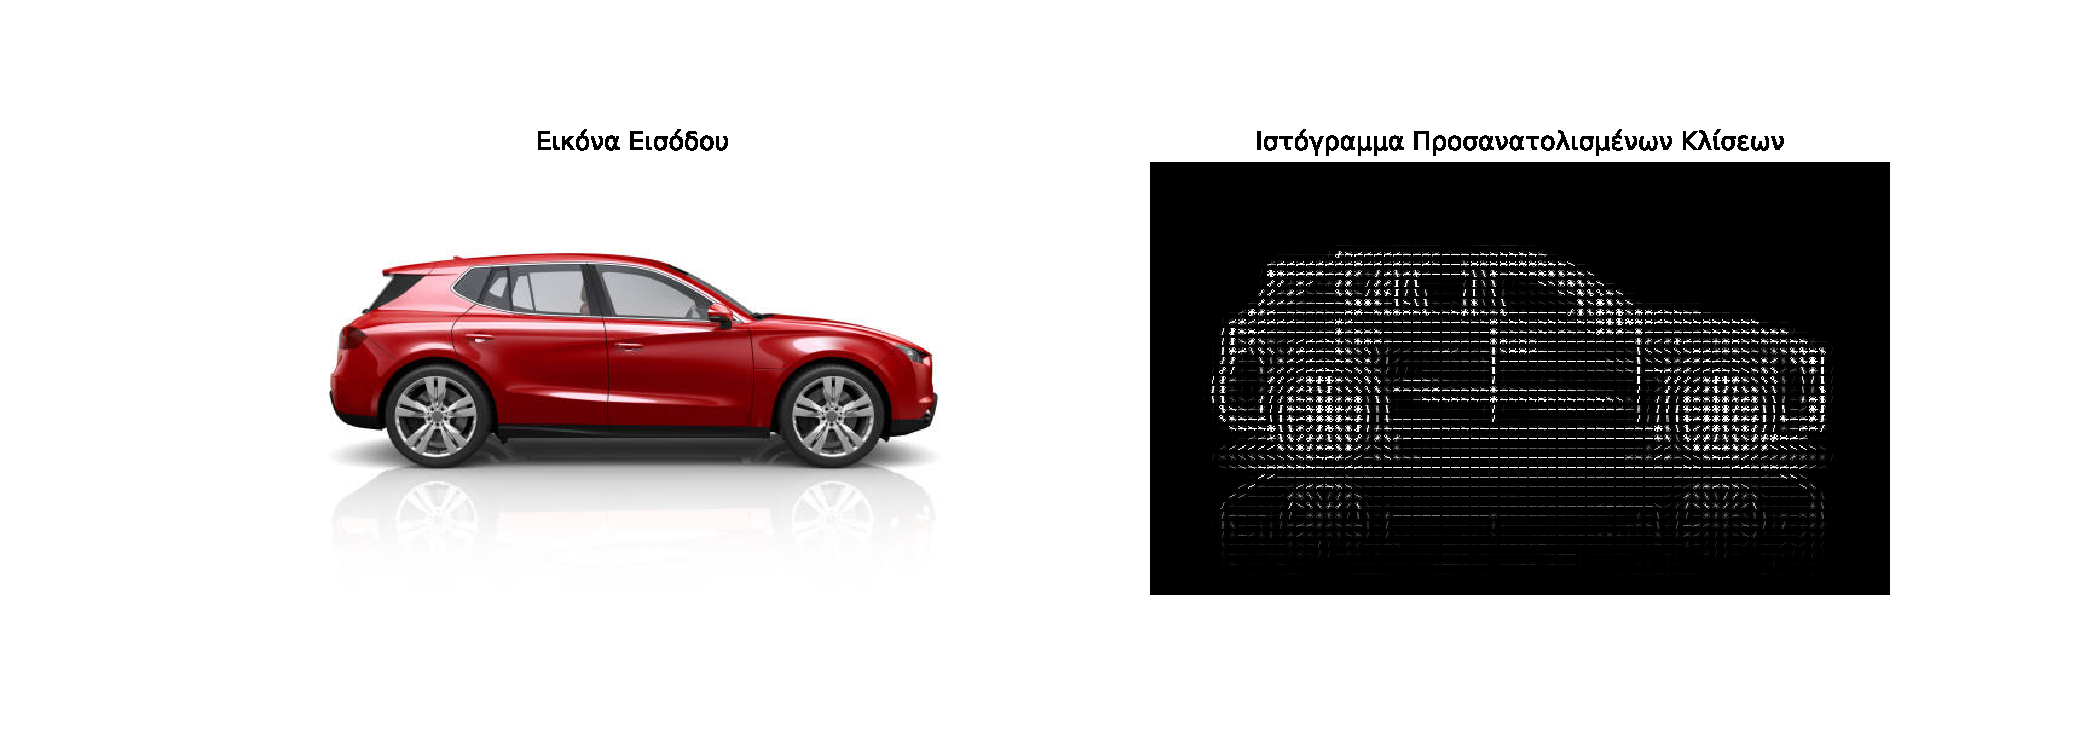
\includegraphics[width=0.95\textwidth]{images/chapter theoritical background/hog_gr.pdf}
  \caption{Παράδειγμα εξαγωγής χαρακτηριστικών σε εικόνα ενός αυτοκινήτου με τη μέθοδο του Ιστογράμματος Προσανατολισμένων Κλίσεων (\en{Histogram of Oriented Gradients}). \textit{Παράχθηκε τοπικά. TODO}} 
  \label{fig:_hog}
\end{figure}

Αν και στο παραπάνω πρόβλημα ήταν σχετικά εύκολη η \textquote{χειρονακτική} εξαγωγή χαρακτηριστικών, υπάρχουν πολλοί χώροι προβλημάτων όπου κάτι τέτοιο είναι από πολύ απαιτητικό έως απίθανο. Ενδεικτικά, σε ένα πρόβλημα οπτικής αναγνώρισης ζώων και αντικειμένων (όπως αυτό του \en{CIFAR-10}\cite{krizhevsky2009learning}) είναι εξαιρετικά δύσκολη η περιγραφή χαρακτηριστικών που θα λαμβάνουν μια αναπαράσταση σε εικονοστοιχεία (\en{pixel}) και θα παράγουν μια χρήσιμη αναπαράσταση. Μολονότι υπάρχουν γενικευμένες μέθοδοι για την εξαγωγή χαρακτηριστικών σε εικόνες όπως αυτή του σχήματος \ref{fig:_hog}, αυτές δεν είναι βέλτιστα προσαρμοσμένες στον χώρο του εκάστοτε προβλήματος. Απόρροια αυτού μεταξύ άλλων είναι η απόρριψη στοιχείων των ακατέργαστων δεδομένων που μπορεί να είναι χρήσιμα (π.χ. σε ένα πρόβλημα αναγνώρισης μάρκας και χρώματος αυτοκινήτου, η μέθοδος Ιστογράμματος Προσανατολισμένων Κλίσεων θα απέρριπτε το χρώμα, στοιχείο χρήσιμο για τον χώρο του προβλήματος). \par

Η λύση για την αντιμετώπιση των προβλημάτων της χειρονακτικής εξαγωγής χαρακτηριστικών είναι η χρήση των αλγορίθμων μηχανικής μάθησης για την εκμάθηση όχι μόνο για της αντιστοίχησης των δεδομένων εκπαίδευσης στην επιθυμητή έξοδο αλλά και των ίδιων των αναπαραστάσεων των δεδομένων. Αν και συνήθως, οι προκύπτουσες αναπαραστάσεις μετά τον μετασχηματισμό των ακατέργαστων δεδομένων δεν είναι κατανοητές από τον άνθρωπο, εφόσον η εκπαίδευση γίνει επιτυχημένα, αποτελούνται από χρήσιμα χαρακτηριστικά (που κωδικοποιούν τους παράγοντες διακύμανσης).
Χαρακτηριστικό παράδειγμα συστήματος για την εκμάθηση χαρακτηριστικών είναι ο Αυτοκωδικοποιητής (\en{Autoencoder}).

\subsection{Πολυεπίπεδα Νευρωνικά Δίκτυα}

Η εκμάθηση χαρακτηριστικών σε συνδυασμό με τις ιδέες του κονεκτιβισμού περί κατανεμημένης αναπαράστασης (βλ. ενότητα \ref{sec:historic_note}) μας οδηγεί αναπόφευκτα στη βαθιά μάθηση (\en{deep learning}). Υπό μια αφαιρετική σκοπιά, πρόκειται για τα λεγόμενα \textquote{πολυεπίπεδα νευρωνικά δίκτυα} τα οποία συνδυάζουν τόσο τον μετασχηματισμό της αναπαράστασης των δεδομένων εισόδου όσο και την αντιστοίχηση αυτών των νέων αναπαραστάσεων στην τιμή εξόδου. Τα συστήματα αυτά, όπως θα δούμε στη συνέχεια, είναι δομημένα από απλές υπολογιστικές μονάδες που τους επιτρέπουν να δημιουργούν σύνθετες αναπαραστάσεις μέσω μιας σειράς από εμφωλευμένες, απλούστερες αναπαραστάσεις. Σημειώνουμε ότι πραγματοποιούν μάθηση με κατασκευή μοντέλου (\en{model\textendash based learning systems}) και χρησιμοποιούνται τόσο σε προβλήματα ταξινόμησης όσο και παλινδρόμησης. Στις επόμενες παραγράφους, θα περιγράψουμε με μεγαλύτερη λεπτομέρεια τον χώρο των νευρωνικών δικτύων\footnote{Για έναν τυπικό ορισμό, παραπέμπουμε τον αναγνώστη στο παράρτημα \ref{chap:definitions}}.

\subsubsection{Δομή Απλών Νευρωνικών Δικτύων}
\label{sec:_vanilla_nn}
Τα Νευρωνικά Δίκτυα στην πιο βασική τους μορφή (\en{Feedforward Neural Networks} ή \en{Multilayer Perceptron}) αποτελούνται από απλούς τεχνητούς νευρώνες διασυνδεδεμένους μεταξύ τους με συνάψεις σχηματίζοντας μια πολυεπίπεδη διάταξη. Το πρώτο επίπεδο ονομάζεται επίπεδο εισόδου (\en{input layer}) ενώ το τελευταίο ονομάζεται επίπεδο εξόδου (\en{output layer}). Όλα τα ενδιάμεσα επίπεδα λέγονται κρυφά επίπεδα (\en{hidden layers}) διότι οι τιμές τους δε δίνονται από τα δεδομένα \cite{goodfellow2016deep}. Στην απλή περίπτωση που εξετάζουμε, κάθε νευρώνας δέχεται ως είσοδο τιμές από όλους τους νευρώνες του αμέσως προηγούμενου επιπέδου (\en{fully connected layer}) και αφού κάνει υπολογισμούς με αυτές στέλνει το αποτέλεσμα σε όλους τους νευρώνες του αμέσως επόμενου επιπέδου.
\par
                  
\begin{figure}[h]
    
    \centering
    \begin{neuralnetwork}[height=4, layerspacing=0.25\textwidth, nodespacing=28mm, nodesize=25pt]
        \newcommand{\mylinktext}[4] {
            % from layer=#1, from node=#2
            % to layer=#3, to node=#4
            $w^{[#3 ]}_{#4#2}$
        }
        % Then assign it:
        \setdefaultlinklabel{\mylinktext}
        \newcommand{\x}[2]{$x_#2$}
        \newcommand{\y}[2]{$\hat{y}_#2$}
        \newcommand{\hfirst}[2]{\small $a^{[1]}_#2$}
        \newcommand{\hsecond}[2]{\small $a^{[2]}_#2$}
        \inputlayer[count=3, bias=false, title=Επίπεδο\\Εισόδου, text=\x]
        \hiddenlayer[count=4, bias=false, title=Κρυφό\\Επίπεδο 1, text=\hfirst] \linklayers
        \hiddenlayer[count=3, bias=false, title=Κρυφό\\Επίπεδο 2, text=\hsecond] \linklayers
        \outputlayer[count=2, title=Επίπεδο\\Εξόδου, text=\y] \linklayers
    \end{neuralnetwork}
    \caption{Διάγραμμα Τεχνητού Νευρωνικού Δικτύου με δύο κρυφά επίπεδα. Οι αγκύλες στους εκθέτες προσδιορίζουν τον αριθμό του επιπέδου. \textit{Παράχθηκε από το \en{LaTeX} πακέτο \href{https://github.com/battlesnake/neural}{\en{neuralnetwork}}. Το πακέτο τροποποιήθηκε και επεκτάθηκε τοπικά.}}
    \label{fig:_vanilla_nn}
\end{figure}

Η αναπαράσταση των νευρωνικών δικτύων γίνεται με έναν γράφο από ακμές (συνάψεις) και κόμβους (νευρώνες ή τιμές εισόδου). Κοιτώντας κανείς το σχήμα \ref{fig:_vanilla_nn} μπορεί να παρατηρήσει πως οι κόμβοι των επιπέδων εισόδου και εξόδου ξεχωρίζουν από τους κόμβους των κρυφών επιπέδων. Αυτό έχει γίνει για να τονιστεί η ξεχωριστή λειτουργία τους. Πιο συγκεκριμένα, στην περίπτωση του επιπέδου εισόδου, αυτό περιέχει τόσους κόμβους όσος είναι και ο αριθμός των χαρακτηριστικών που περιγράφουν το κάθε παράδειγμα (δηλαδή όσο και το μήκος του διανύσματος εισόδου). Ουσιαστικά, οι κόμβοι εισόδου απλά λαμβάνουν τις τιμές των χαρακτηριστικών και, χωρίς να τις μεταβάλλουν, τις δρομολογούν στους κόμβους του επόμενου επιπέδου (για αυτό και αποφεύγεται η επωνομασία αυτών των κόμβων ως νευρώνες). Στην περίπτωση του επιπέδου εξόδου, ο αριθμός των κόμβων είναι τόσος όσος και ο αριθμός των χαρακτηριστικών για την περιγραφή της πρόβλεψης (τόσο όσο το μήκος του διανύσματος εξόδου). Οι κόμβοι εξόδου συνήθως επιβάλουν περιορισμούς στις τιμές των χαρακτηριστικών εξόδου ώστε αυτές να ανήκουν σε ένα φραγμένο σύνολο αριθμών (π.χ. το [0,1]).
\par

Ένα νευρωνικό δίκτυο χωρίς κρυφά επίπεδα δε διαφέρει από έναν γραμμικό ταξινομητή. Είναι γεγονός ότι οι εκπληκτικές δυνατότητες των νευρωνικών δικτύων αποδίδονται στα κρυφά επίπεδα. Χάρη σε αυτά είναι δυνατή η σταδιακή σύνθεση αφηρημένων αναπαραστάσεων από επίπεδο σε επίπεδο που κωδικοποιούν τους παράγοντες διακύμανσης. Τα κρυφά επίπεδα τα απαρτίζουν οι κόμβοι κρυφού επιπέδου\footnote{Εφεξής θα αποκαλούνται ως κόμβοι.}. Ο κάθε ένας από αυτούς υπολογίζει την έξοδο μιας μη γραμμικής συνάρτησης με είσοδο ένα γραμμικό συνδυασμό των τιμών των κόμβων του προηγούμενου επιπέδου. Αξίζει να αναφερθεί στο σημείο αυτό πως δεν υπάρχει κάποιος συγκεκριμένος περιορισμός για τον αριθμό των κόμβων των κρυφών επιπέδων. \par

Η φορμαλιστική περιγραφή των παραμέτρων\footnote{Πρόκειται για μεταβλητές των οποίων οι τιμές μαθαίνονται κατά τη διάρκεια της εκπαίδευσης. Έτσι το νευρωνικό δίκτυο λέμε ότι προσαρμόζεται στα δεδομένα.} και των υπολογισμών που λαμβάνουν χώρα κατά τη διαδικασία πρόβλεψης ενός νευρωνικού δικτύου περιγράφονται παρακάτω. \par

Έστω ένα παράδειγμα εισόδου το οποίο περιγράφεται από $n_x$ χαρακτηριστικά με το διάνυσμα \(X = \big[x_1, x_2, x_3, \dots, x_{n_{x}}]^T\). Όλα τα δεδομένα εκπαίδευσης, έστω \en{\textit{M}}, μπορούν να ομαδοποιηθούν σε έναν πίνακα $\boldsymbol{X}$ ως εξής: 
\begin{equation}
    \boldsymbol{X} =
    \underset{(n_x \times M)}{\begin{bmatrix}
        |&|&&| \\
        X^{(1)} & X^{(2)} & \dots & X^{(M)}\\
        |&|&&|
    \end{bmatrix}}.
\end{equation}
\textit{Όπου οι παρενθέσεις στους εκθέτες δηλώνουν τον αριθμό του παραδείγματος.}\par

Αφού προσδιορίσαμε μια μαθηματική αναπαράσταση για τα δεδομένα εισόδου, πάμε να προσδιορίσουμε με φορμαλιστικό τρόπο τις παραμέτρους του νευρωνικού δικτύου. Με $L$ θα συμβολίζουμε τον αριθμό των επιπέδων του νευρωνικού δικτύου (χωρίς να μετράμε το επίπεδο εισόδου). Για παράδειγμα, στο δίκτυο του σχήματος \ref{fig:_vanilla_nn} ισχύει $L=3$. Επίσης, ο αριθμός των κόμβων ενός επιπέδου, έστω $l$, θα συμβολίζεται με $n^{[l]}$. Προφανώς, θα ισχύει ότι $l \in [0,L]$. Στο παράδειγμα του σχήματος \ref{fig:_vanilla_nn} ισχύει $n^{[0]}=n_x=3, n^{[1]}=4, n^{[2]}=3, n^{[3]}=n_y=2$. Έχοντας δώσει έναν συμβολισμό ορισμένων βασικών υπερπαραμέτρων\footnote{Σε αντίθεση με τις παραμέτρους, οι υπερπαράμετροι είναι μεταβλητές που ορίζει ο χρήστης και δε μεταβάλλονται κατά την εκπαίδευση. Ονομάζονται έτσι διότι ελέγχουν έμμεσα τις τιμές των παραμέτρων.}, μπορούμε αποδώσουμε φορμαλιστικά τις παραμέτρους του δικτύου οι οποίες είναι:
\begin{itemize}
    \item Τα βάρη των ακμών (\en{weights}) που συνδέουν δύο διαδοχικά επίπεδα.\\
    Τα βάρη μεταξύ διαδοχικών επιπέδων $l-1$ και $l$ μπορούμε να τα οργανώσουμε σε μια μορφή πίνακα ως εξής:
    \begin{equation}
        \boldsymbol{W^{[l]}} =
        \underset{(n^{[l]} \times n^{[l-1]})}{\begin{bmatrix}
            w^{[l]}_{11}&w^{[l]}_{12}& \dots&w^{[l]}_{1n^{[l-1]}} \\[0.5em]
            w^{[l]}_{21}&w^{[l]}_{22}& \dots&w^{[l]}_{2n^{[l-1]}}\\[0.3em]
            \vdots & \vdots& \ddots& \vdots \\[0.3em]
            w^{[l]}_{n^{[l]}1}&w^{[l]}_{n^{[l]}2}& \dots&w^{[l]}_{n^{[l]}n^{[l-1]}}\\[0.5em]
        \end{bmatrix}}.
    \end{equation}
    \item Τα δυναμικά πόλωσης (\en{biases}) του κάθε νευρώνα. \\
    Όπως είναι λογικό, οι κόμβοι του επιπέδου $0$ (επίπεδο εισόδου) δε διαθέτουν δυναμικά πόλωσης. Για όλους τους άλλους κόμβους σε κάθε επίπεδο (έστω $l$) έχουμε το εξής διάνυσμα στήλη:
    \begin{equation}
        \boldsymbol{b^{[l]}} = 
        \underset{(n^{[l]} \times 1)}{
            \begin{bmatrix}
                b^{[l]}_1 \\[0.3em]
                b^{[l]}_2 \\[0.3em]
                \vdots \\[0.3em]
                b^{[l]}_{n^{[l]}}\\[0.3em]
            \end{bmatrix}}.
    \end{equation}
\end{itemize}

Τώρα, είμαστε σε θέση να περιγράψουμε τους υπολογισμούς που πραγματοποιεί κάθε νευρώνας. Για τον σκοπό αυτό, παρουσιάζουμε μια αναπαράστασή του στο σχήμα \ref{fig:_neural_node}. \par

\begin{figure}[h]
    \centering
\begin{tikzpicture}[
    init/.style={
      draw,
      circle,
      inner sep=2pt,
      font=\Huge,
      join = by -latex
    },
    squa/.style={
      draw,
      inner sep=2pt,
      font=\Large,
      join = by -latex
    },
    start chain=2,node distance=13mm
    ]
    \node[on chain=2] 
      (x2) {$x_2$};
    \node[on chain=2,join=by o-latex] 
      (w2) {$w_2$};
    \node[on chain=2,init] (sigma) 
      {$\displaystyle\Sigma$};
    \node[on chain=2,squa,label=above:{\parbox{3cm}{\centering Συνάρτηση \\ Ενεργοποίησης}}]   
      {$f$};
    \node[on chain=2,label=below:Έξοδος,join=by -latex] 
      {$y$};
    \begin{scope}[start chain=1]
    \node[on chain=1] at (0,1.3cm) 
      (x1) {$x_1$};
    \node[on chain=1,join=by o-latex] 
      (w1) {$w_1$};
    \end{scope}
    \begin{scope}[start chain=3]
    \node[on chain=3] at (0,-1.8cm) 
      (x3) {$x_n$};
    \node[on chain=3,label=below:Βάρη,join=by o-latex] 
      (w3) {$w_n$};
    \end{scope}
    \node[label=above:\parbox{2cm}{\centering Πόλωση \\ $b$}] at (sigma|-w1) (b) {};
    
    \draw[-latex] (w1) -- (sigma);
    \draw[-latex] (w3) -- (sigma);
    \draw[o-latex] (b) -- (sigma);
    \draw[loosely dotted] (w2) -- (w3);
    \draw[loosely dotted] (x2) -- (x3);
    \draw[decorate,decoration={brace,mirror}] (x1.north west) -- node[left=10pt] {Είσοδοι} (x3.south west);
    \end{tikzpicture}
    \caption{Διάγραμμα ενός τεχνητού νευρώνα. \textit{Παράχθηκε από το πακέτο \en{tikz}.}}
    \label{fig:_neural_node}
\end{figure}

Εσωτερικά ο κάθε νευρώνας δέχεται ως είσοδο τις τιμές των νευρώνων του προηγούμενου επιπέδου ή (στην περίπτωση του δεύτερου επιπέδου) τις τιμές του παραδείγματος εκπαίδευσης και πραγματοποιεί υπολογισμούς με αυτές για να παράξει μια τιμή εξόδου. Την κάθε τιμή εισόδου τη συμβολίζουμε με $x$ ενώ την τιμή εξόδου του μεμονωμένου νευρώνα τη συμβολίζουμε με $y$. Η πράξη που επιτελείται εσωτερικά είναι:
\begin{equation}
y = f\Big(\sum_{i = 1}^{n} w_i \times x_i  +  b\Big)
\end{equation}
Όπου $f(x)$ είναι η συνάρτηση ενεργοποίησης (\en{activation function}). Αυτές οι συναρτήσεις, μεταξύ άλλων, επιτρέπουν στο σύστημα να μοντελοποιήσει μη γραμμικές σχέσεις εισόδου\textendash εξόδου. Πρωταρχικά, χρησιμοποιούνταν για να μοντελοποιήσουν τη μη\textendash γραμμική, δύτιμη έξοδο των βιολογικών νευρώνων. Στον χώρο των υπολογιστών όμως, έγιναν γρήγορα αντιληπτά τα πρακτικά πλεονεκτήματα της κατασκευής βιολογικών νευρώνων με έξοδο συνεχείς τιμές που ανήκουν στον χώρο των πραγματικών αριθμών\footnote{Αυτός είναι και ο λόγος που ο όρος \textquote{ενεργοποίηση} θέλει προσοχή όταν αναφερόμαστε σε τεχνητούς νευρώνες. Στην περίπτωση χρήσης του όρου σε ένα τέτοιο πλαίσιο, θα εννοούμε ότι ο νευρώνας αυτός έχει σχετικά μεγαλύτερη τιμή εξόδου και συνάμα έχει μεγαλύτερη \textquote{ευθύνη} στη διαμόρφωση της τελικής εξόδου.}. Έτσι, από τη βηματική συνάρτηση (όπως αυτή στο \en{Perceptron} του \en{H. Rosenblat} \cite{rosenblatt1958perceptron}) που έχει ως σύνολο τιμών το ${0,1}$, άρχισε να γίνεται χρήση άλλων με συνεχές πεδίο τιμών όπως για παράδειγμα η σιγμοειδής ή η υπερβολική συνάρτηση εφαπτομένης (\en{tanh}) κ.τ.λ. \par

Στο σημείο αυτό να αναφέρουμε πως το όρισμα της συνάρτησης ενερογοποίησης, δηλαδή την ποσότητα \(\sum_{i = 1}^{n} w_i \times x_i  +  b\) τη συμβολίζουμε με $z$ ενώ την τιμή του $y$ την ονομάζουμε και τιμή ενεργοποίησης (συμβολίζοντάς τη με $a$). Στην περίπτωση δε που ο νευρώνας ανήκει στο επίπεδο εξόδου, την τιμή $y$ την ονομάζουμε τιμή πρόβλεψης και την αναπαριστούμε με το γράμμα $\hat{y}$. \par

Κοιτώντας τώρα εποπτικά τη διαδικασία παραγωγής νέων προβλέψεων ενός τυπικού νευρωνικού δικτύου, μπορούμε να την περιγράψουμε χρησιμοποιώντας αναπαράσταση με διανύσματα (\en{vector notation}). Αναλυτικότερα, αν συγκεντρώσουμε όλες τις τιμές ενεργοποίησης $a$ ενός επιπέδου $l$ σε ένα διάνυσμα \(A^{[l]} = \big[a_1^{[l]}, a_2^{[l]}, a_3^{[l]}, \dots, a_{n^{[l]}}^{[l]}]^T\) και κάνουμε το ίδιο για τα ορίσματα $z$ των συναρτήσεων ενεργοποίησης δηλαδή \(Z^{[l]} = \big[z_1^{[l]}, z_2^{[l]}, z_3^{[l]}, \dots, z_{n^{[l]}}^{[l]}]^T\) τότε συνολικά, γράφουμε:
\begin{itemize}
  \item Τα στοιχεία $a$ προκύπτουν από τα στοιχεία $z$ του ίδιου επιπέδου ως εξής:
    \begin{equation} \label{eq:1}
      A^{[l]} = F^{[l]}\big(Z^{[l]}\big)
    \end{equation}
    \textit{Όπου η συνάρτηση $F$ εφαρμόζει την $f$ σε κάθε στοιχείο του ορίσματός της ξεχωριστά (\en{elementwise}).}
  \item Τα στοιχεία $z$ υπολογίζονται από τα στοιχεία $a$ του προηγούμενου επιπέδου μέσω της σχέσης:
    \begin{equation} \label{eq:2}
      Z^{[l]} = W^{[l]} \times A^{[l-1]} + \boldsymbol{b}^{[l]}
    \end{equation}
    \textit{Όπου $A^{0} = X$, το διάνυσμα χαρακτηριστικών ενός παραδείγματος ενώ $A^{[L]} = \hat{Y}$ το διάνυσμα εξόδου.}
\end{itemize}

Η ανωτέρω ανάλυση πραγματοποιήθηκε για ένα μεμονωμένο παράδειγμα. Θα βοηθήσει για την επεξήγηση του τρόπου εκπαίδευσης των νευρωνικών δικτύων αν παρουσιάσουμε τώρα μια μορφή μαθηματικών τύπων που συγκεντρώνουν τις τιμές όλων των παραδειγμάτων του συνόλου εκπαίδευσης. Θυμηθήτε, ότι κάθε στήλη του πίνακα δεδομένων εισόδου $\boldsymbol{X}$ περιέχει ένα διάνυσμα παραδείγματος με αποτέλεσμα ο αριθμός των στηλών να ισούται με τον αριθμό των παραδειγμάτων, $M$. Κατά αυτόν τον τρόπο έχουμε:
\begin{itemize}
  \item Για τα $z$ ενός επιπέδου $l$ για το κάθε παράδειγμα εισόδου:
  \begin{equation}
    \boldsymbol{Z^{[l]}} =
    \underset{(n^{[l]} \times M)}{\begin{bmatrix}
        |&|&&| \\
        Z^{[l](1)} & Z^{[l](2)} & \dots & Z^{[l](M)}\\
        |&|&&|
    \end{bmatrix}}.
  \end{equation}
  \item Αντίστοιχα, για τα $a$ ενός επιπέδου $l$ για το κάθε παράδειγμα εισόδου:
  \begin{equation}
    \boldsymbol{A^{[l]}} =
    \underset{(n^{[l]} \times M)}{\begin{bmatrix}
        |&|&&| \\
        A^{[l](1)} & A^{[l](2)} & \dots & A^{[l](M)}\\
        |&|&&|
    \end{bmatrix}}.
  \end{equation}
  Όπως προκύπτουν από τις σχέσεις 
  \begin{equation}\label{eq:_fw_z}
    \underset{(n^{[l]} \times M)}{\boldsymbol{Z}^{[l]}} = \underset{(n^{[l]} \times n^{[l-1]})}{W^{[l]}} \times \underset{(n^{[l-1]} \times M)}{\boldsymbol{A}^{[l-1]}} + \underset{(n^{[l]} \times 1)}{\boldsymbol{b}^{[l]}}
  \end{equation}
   και 
  \begin{equation}\label{eq:fw_a}
    \underset{(n^{[l]} \times M)}{\boldsymbol{A}^{[l]}} = F^{[l]}\big(\underset{(n^{[l]} \times M)}{\boldsymbol{Z}^{[l]}}\big)
  \end{equation} 
  αντίστοιχα, όπου η μόνη διαφορά με τις \ref{eq:2}, \ref{eq:1} είναι ότι αντικαταστήσαμε τα διανύσματα στήλες $Z$ και $A$ με τους πίνακες $\boldsymbol{Z}$ και $\boldsymbol{A}$. Και πάλι, $\boldsymbol{A}^{0} = \boldsymbol{X}$, ο πίνακας όλων των δεδομένων εισόδου ενώ $\boldsymbol{A}^{[L]} = \boldsymbol{\hat{Y}}$ το σύνολο διανυσμάτων εξόδου.
\end{itemize}

\subsubsection{Εκπαίδευση Νευρωνικών Δικτύων}

Στην προηγούμενη παράγραφο διατυπώσαμε τους μαθηματικούς τύπους σύμφωνα με τους οποίους ένα νευρωνικό δίκτυο, δοθέντος ενός συνόλου δεδομένων $\boldsymbol{X}$ παράγει ένα σύνολο από προβλέψεις $\boldsymbol{\hat{Y}}$. Η διαδικασία αυτή ονομάζεται και πρόσθια διάδοση (\en{forward propagation}). Παρόλα αυτά, δεν αναφερθήκαμε καθόλου στη διαδικασία μάθησης του δικτύου. Υποθέσαμε σιωπηρά ότι αυτό ήταν ήδη εκπαιδευμένο και οι παράμετροί του (τα βάρη και τα δυναμικά πόλωσης) ήταν σταθερά. Με τη μέχρι τώρα παρουσίαση, το νευρωνικό δίκτυο δεν είναι τίποτα άλλο παρά μια μη γραμμική συνάρτηση. Σε αυτήν την παράγραφο όμως, θα κάνουμε τη σύνδεση των νευρωνικών δικτύων με τη μηχανική μάθηση αναλύοντας τον μηχανισμό εκπαίδευσής τους. \par

Όπως έχουμε αναφέρει, τα νευρωνικά δίκτυα είναι πολυδύναμα συστήματα μηχανικής μάθησης βασισμένα σε μοντέλο ενώ καμία επιπλέον υπόθεση δεν μπορεί να γίνει εκ των προτέρων. Με άλλα λόγια, υπάρχουν νευρωνικά δίκτυα που ανήκουν σε όλες τις υπόλοιπες κατηγορίες που παρατέθηκαν στην ενότητα \ref{sec:_ML_varieties}. Παρόλα αυτά, για τον σκοπό της παρούσας παραγράφου, θα περιορίσουμε αυτά τα πολυδύναμα συστήματα σε αυτά που πραγματοποιούν επιβλεπόμενη μάθηση. Ευτυχώς, αυτή είναι η πιο βασική κατηγορία και οι ιδέες που θα παρουσιαστούν υπό αυτή εύκολα μεταφέρονται και στις υπόλοιπες. \par

Στο πλαίσιο της επιβλεπόμενης μάθησης, εκτός από το σύνολο δεδομένων εισόδου $\boldsymbol{X}$ παρέχεται, και ένα σύνολο δεδομένων εξόδου $\boldsymbol{Y}$. Το τελευταίο αποτελείται από ένα επιθυμητό διάνυσμα (ή τιμή) στόχο για κάθε παράδειγμα του συνόλου δεδομένων εισόδου. Έτσι, (όπως αναφέρουμε και στο παράρτημα \ref{chap:definitions}) σχηματίζονται ζεύγη διανυσμάτων εισόδου\textendash επιθυμητής εξόδου. Στόχος του νευρωνικού δικτύου σε αυτήν την περίπτωση είναι να δημιουργήσει μια συνάρτηση που θα κάνει την αντιστοίχηση από τα παραδείγματα $X$ στις προβλέψεις του στόχου, $\hat{Y}$ να είναι όσο πιο πιστή γίνεται στην αντιστοίχηση $X$ σε $Y$. Με μαθηματικούς όρους, έστω η συνάρτηση του νευρωνικού δικτύου: $\mathcal{F}(X;\overline{W},\overline{b})$, όπου με $\overline{W}$ και $\overline{b}$ συμβολίζεται αντίστοιχα το σύνολο των βαρών και δυναμικών πόλωσης σε όλα τα επίπεδα\footnote{Το σύμβολο \textquote{\en{;}} διαβάζεται ως \textquote{παραμετροποιημένο από}.}. Θέλουμε για τη συνάρτηση $\mathcal{F}(X;\overline{W},\overline{b}):X \rightarrow \hat{Y}$ να ισχύει $\mathcal{F}(X;\overline{W^*},\overline{b^*}) \approx \mathcal{G}(X)$ όπου $\mathcal{G}$ η (άγνωστη) συνάρτηση από την οποία (θεωρητικά) παράχθηκαν τα ζεύγη εισόδου\textendash εξόδου και οι δείκτες αστερίσκοι συμβολίζουν τις ιδανικές τιμές των παραμέτρων\footnote{Ουσιαστικά, το κύριο πρόβλημα που καλούνται να λύσουν τα νευρωνικά δίκτυα (και τα συστήματα μηχανικής μάθησης γενικότερα) πηγάζει από το γεγονός ότι η συνάρτηση $\mathcal{G}$ είναι άγνωστη. Αντ' αυτής, διατίθεται ένα σύνολο ζευγών $X-Y$ που αποτελεί υποσύνολο του πληθυσμού όλων των δυνατών εισόδων και το σύστημα επιδιώκει από αυτό το υποσύνολο να μάθει να γενικεύει σε παραδείγματα που δεν έχει δει. Αυτός είναι και ο λόγος που, υπό την αυστηρά μαθηματική έννοια, η διαδικασία της εκπαίδευσης αποκαλείται και συμπερασματολογία (\en{inference}). Σε τελική ανάλυση, τα περισσότερα νευρωνικά δίκτυα εκπαιδεύονται χρησιμοποιώντας συμπερασματολογία βασισμένη στη μέγιστη πιθανοφάνεια (\en{maximum likelihood inference})\cite{goodfellow2016deep}. Δηλαδή, προσπαθούν να μεγιστοποιήσουν την ποσότητα $p(y|x;\overline{W},\overline{b})$ και γιαυτό ονομάζονται μοντέλα διάκρισης (\en{descriminative models}).}.\par

Για να προσαρμόσουμε με βέλτιστο τρόπο τις παραμέτρους του μοντέλου στην εμπειρία απαιτείται (σύμφωνα με τον ορισμό της μηχανικής μάθησης) μια μετρική η οποία θα μας δείχνει πόσο κατάλληλη είναι η προσέγγισή μας (\en{fittness}). Αυτή η μετρική ονομάζεται συνάρτηση απώλειας (\en{loss function}) και στη γενική της μορφή είναι \( \mathsf{L}(\hat{Y},Y) = \mathsf{L}(\mathcal{F}(\boldsymbol{X};\overline{W},\overline{b}),Y)\). Ανάλογα με το είδος του προβλήματος, τυπικές συναρτήσεις απώλειας είναι:
\begin{itemize}
  \item H (\en{binary cross entropy loss}): $\mathsf{L}(\hat{Y},Y) = -\frac{1}{M}\sum_{i = 1}^{M} \big(y^{(i)}\log(\hat{y}^{(i)}) + (1 - y^{(i)})\log(1 - \hat{y}^{(i)})\big)$ \\στην περίπτωση προβλήματος δυαδικής ταξινόμησης (όπου η έξοδος $\hat{y}$ είναι ίση με την πιθανότητα το παράδειγμα $x$ να ανήκει στην κλάση 1)
  \item Η (\en{mean square error loss}): $\mathsf{L}(\hat{Y},Y) = \frac{1}{M}\sum_{i = 1}^{M}{\left\lVert y^{(i)} - \hat{y}^{(i)}\right\rVert}^2 $\\ στην περίπτωση προβλήματος παλινδρόμησης (όπου $\left\lVert x \right\rVert$ συνήθως είναι η $L2$ νόρμα).
\end{itemize}
Να σημειώσουμε ότι ορίσαμε τη συνάρτηση απώλειας ώστε να δέχεται ένα σύνολο από προβλέψεις και επιθυμητές τιμές στόχους. Αντίστοιχα, θα μπορούσαμε να ορίσουμε συνάρτηση απώλειας που συγκρίνει την πρόβλεψη με την έξοδο στόχο ενός συγκεκριμένου παραδείγματος (και να μην αθροίζει όλα τα παραδείγματα). Τότε, θα είχαμε \( L(\hat{y},y) = L(\mathcal{F}(X;\overline{W},\overline{b}),y)\). \par

Έχοντας στη διάθεσή μας μια μετρική απόδοσης, το πρόβλημα της εκπαίδευσης του νευρωνικού δικτύου μπορεί να διατυπωθεί ως πρόβλημα βελτιστοποίησης. Με μαθηματικούς όρους έχουμε:
\begin{equation}
  \overline{W^*},\overline{b^*} = \underset{\overline{W},\overline{b}}{\mathrm{argmax}}(\mathsf{L}(\mathcal{F}(\boldsymbol{X};\overline{W},\overline{b}),Y))
\end{equation}
Εξετάζοντας τη μετρική $\mathsf{L}$ σαν συνάρτηση των $\overline{W}$ και $\overline{b}$, για την επίλυση του ανωτέρω προβλήματος αρκεί να βρούμε το σημείο στον χώρο των παραμέτρων που την ελαχιστοποιεί. Λόγω των μη γραμμικών στοιχείων όμως, δεν υπάρχει κλειστός τύπος (\en{closed form}) για την εύρεση του σημείου αυτού. Όπως φαίνεται και από το σχήμα \ref{fig:_gd01}, η συνάρτηση απώλειας είναι μη κυρτή. Αυτό μας οδηγεί στη χρήση επαναληπτικών μεθόδων για την εύρεση κάποιου (τοπικού) ελάχιστου. \par

\begin{figure}[h]
  \centering
  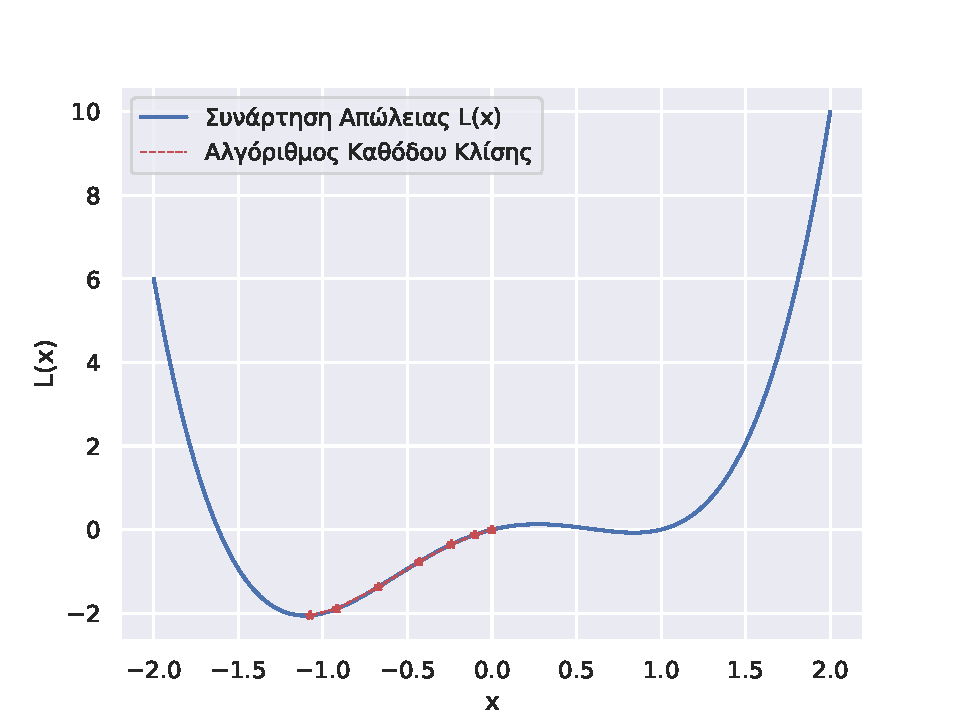
\includegraphics[width=0.7\textwidth]{images/chapter theoritical background/gd_init_at_plus0point1.pdf}
  \caption{Γραφική παράσταση στην οποία εφαρμόζεται ο αλγόριθμος καθόδου κλίσης σε μια μη κυρτή συνάρτηση με μια παράμετρο (την $x$). \todo[inline]{Να προσθέσω λινκ σε κώδικα.} Παράχθηκε τοπικά. }
  \label{fig:_gd01}
\end{figure}

Ο πιο δημοφιλής αλγόριθμος για αυτόν τον σκοπό είναι ο αλγόριθμος καθόδου κλίσης (\en{gradient descent}). Σύμφωνα με τον αλγόριθμο αυτό, πραγματοποιούνται επαναλαμβανόμενα βήματα \textquote{καθόδου} προς την κατεύθυνση με τη μεγαλύτερη κλίση. Διαισθητικά, φαίνεται λογικό σε κάθε βήμα να υπολογίζουμε σημειακά την κλίση της συνάρτησης που θέλουμε να ελαχιστοποιήσουμε και να κινούμαστε προς την κατεύθυνση με τη μικρότερη κλίση. Πιο συγκεκριμένα, πρώτα αρχικοποιούνται ανεξάρτητα όλες οι παράμετροι σε τυχαίες τιμές $\overline{W}_0$, $\overline{b}_0$ και έπειτα ξεκινά μια επαναληπτική διαδικασία όπου σε κάθε βήμα αυτής (έστω $i$):
\begin{enumerate}
  \item Υπολογίζονται οι μερικοί παράγωγοι (η κλήση) της συνάρτησης απώλειας ως προς όλες τις παραμέτρους σημειακά:
    \begin{equation}
      dw_i = \left.\frac{\partial \mathsf{L(\overline{W},\overline{b})}}{\partial w}\right\rvert_{(\overline{W},\overline{b})=(\overline{W}_{i-1},\overline{b}_i-1)}, \forall{w}
    \end{equation}
    και
    \begin{equation}
    db_i = \left.\frac{\partial \mathsf{L(\overline{W},\overline{b})}}{\partial b}\right\rvert_{(\overline{W},\overline{b})=(\overline{W}_{i-1},\overline{b}_i-1)}, \forall{b}
    \end{equation}
    Όπου $\mathsf{L(\overline{W},\overline{b})}$ η συνάρτηση απώλειας υπολογισμένη για ένα σύνολο δεδομένων $\boldsymbol{X}$ υπό τις παραμέτρους $\overline{W},\overline{b}$.
    Συνοπτικά, αν συγκεντρώσουμε όλες τις παραμέτρους $\overline{W}$ και $\overline{b}$ στο διάνυσμα στήλη $\overline{W_{all}}$ τότε γράφουμε:
    \begin{equation}
      {d \overline{W_{all}}}_i = \left.\nabla{\mathsf{L(\overline{W_{all}})}}\right\rvert_{\overline{W_{all}}=\overline{W_{all}}_{i-1}}
    \end{equation}
  \item Μετακινείται το σημείο στον χώρο παραμέτρων προς την κατεύθυνση της μεγαλύτερης κλίσης σύμφωνα με τον κανόνα ενημέρωσης (\en{update rule}) των παραμέτρων\footnote{Φανταστείτε τις παραγώγους ως \textquote{ευθύνες} της κάθε παραμέτρου για τις σωστές ή λάθος προβλέψεις. Όσο πιο μεγάλη η παράγωγος, τόσο πιο καθοριστικό ρόλο παίζει η μεταβλητή στη διαμόρφωση της τιμής της συνάρτησης απώλειας.}. Ο κανόνας είναι ο εξής:
  \begin{equation}
    w_i = w_{i-1} - \alpha \times dw_i, \forall{w} \end{equation}
    και
    \begin{equation} b_i = b_{i-1} - \alpha \times db_i, \forall{b}
    \end{equation}
    Όπου $\alpha$ ο ρυθμός μάθησης (\en{learning rate}): μια υπερπαράμετρος που καθορίζει το μέγεθος του βήματος κατά την ενημέρωση των παραμέτρων. Αντίστοιχα με πριν, συνοπτικά, έχουμε:
    \begin{equation}
      {\overline{W_{all}}}_i = {\overline{W_{all}}}_{i-1} - \alpha \times {d \overline{W_{all}}}_i
    \end{equation}
\end{enumerate} 
Ο αλγόριθμος τελειώνει είτε όταν οι ενημερώσεις είναι πλέον αμελητέες και η τιμή της συνάρτησης απώλειας δε μειώνεται άλλο από επανάληψη σε επανάληψη (ο αλγόριθμος έχει βρει ένα τοπικό ελάχιστο) είτε όταν ξεπεραστεί ο μέγιστος αριθμός επαναλήψεων.\par

\begin{figure}[h]
  \centering
  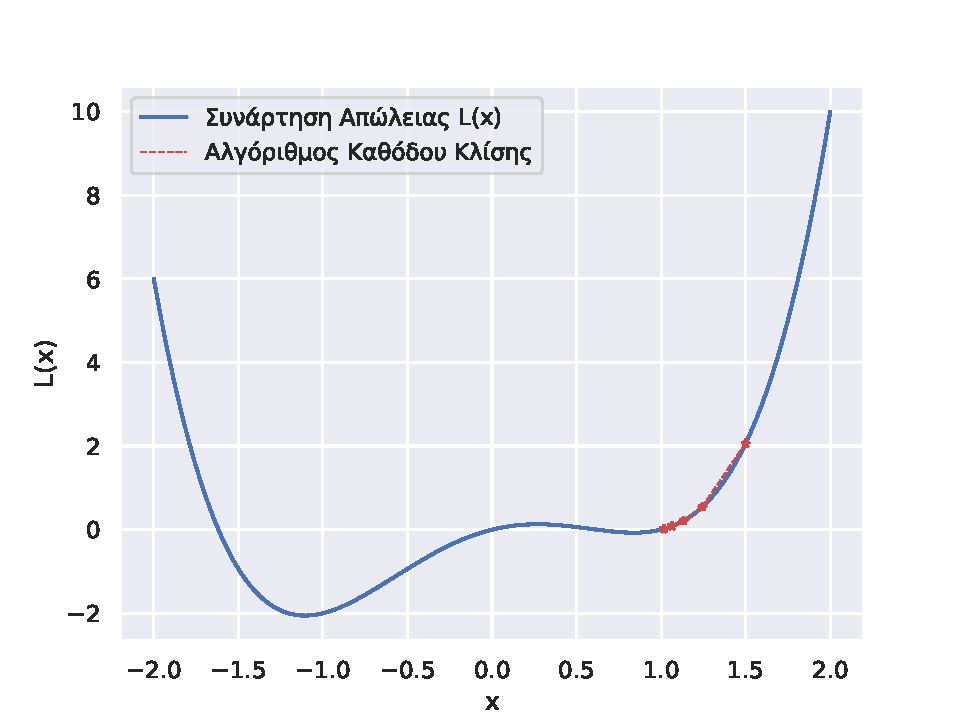
\includegraphics[width=0.7\textwidth]{images/chapter theoritical background/gd_init_at_plus1point5.pdf}
  \caption{Γραφική παράσταση στην οποία εφαρμόζεται ο αλγόριθμος καθόδου κλίσης σε μια μη κυρτή συνάρτηση με μια παράμετρο (την $x$) αρχικοποιημένη όμως στην τιμή 1.5 με αποτέλεσμα να βρίσκεται ένα τοπικό ελάχιστο.}
  \label{fig:_gd15}
\end{figure}

Να σημειώσουμε ότι ο αλγόριθμος καθόδου κλίσης δε βρίσκει πάντα το ολικό ελάχιστο της συνάρτησης. Ανάλογα με την αρχικοποίηση των παραμέτρων και τις τιμές των υπερπαραμέτρων (ρυθμός μάθησης, αριθμός επαναλήψεων) οδηγούμαστε κάθε φορά σε διαφορετικά αποτελέσματα. Για παράδειγμα, στο σχήμα \ref{fig:_gd15} αρχικοποιήσαμε την τιμή της παραμέτρου $x$ με την τιμή +1.5 με αποτέλεσμα ο αλγόριθμος να τερματίσει στο τοπικό ελάχιστο της συνάρτησης. Ανεξάρτητα από τον αριθμό επαναλήψεων, δε θα εντόπιζε ποτέ το ολικό ελάχιστο υπό αυτήν την αρχικοποίηση. Η αδυναμία εγγύησης για την εύρεση του ολικού ελαχίστου αποτελεί τον λόγο για τον οποίο σε αρκετά προβλήματα μηχανικής μάθησης οι αλγόριθμοι εκπαιδεύονται πολλές φορές με διαφορετική όμως αρχικοποίηση των παραμέτρων τους. Ευτυχώς, στα πολυεπίπεδα νευρωνικά δίκτυα δεν ενδιαφέρει η εύρεση του ολικού ελαχίστου\footnote{Καθώς οδηγεί σε \en{overfitting}.} αλλά ενός τοπικού ελαχίστου \cite{choromanska2015loss}.\par

Ο αλγόριθμος της καθόδου κλίσης δε θα χρησίμευε στην εκπαίδευση των νευρωνικών δικτύων αν δεν υπήρχε η δυνατότητα αποδοτικού υπολογισμού των μερικών παραγώγων. Ευτυχώς, τη λειτουργία αυτή την επιτελεί η μέθοδος οπισθοδιάδοσης σφάλματος (\en{back propagation}). Με λίγα λόγια, πρόκειται για μια μέθοδο η οποία χρησιμοποιώντας τον κανόνα της αλυσίδας υπολογίζει την παράγωγο της συνάρτησης απώλειας ως προς όλες τις παραμέτρους του δικτύου (σημειακά), ξεκινώντας από αυτές του τελευταίου επιπέδου και τερματίζοντας σε αυτές του πρώτου.\par

Παρακάτω παρατίθενται οι υπολογισμοί που λαμβάνουν χώρα κατά τη διάρκεια εύρεσης των μερικών παραγώγων ως προς τις παραμέτρους ενός επιπέδου $L-1$ μέσω της οπισθοδιάδοσης σφάλματος για την $i$\textendash οστή επανάληψη του αλγορίθμου καθόδου κλίσης (με δεδομένα εισόδου ένα σύνολο από $M$ παραδείγματα). Αν και οι παράγωγοι υπολογίζονται σημειακά για τις τιμές των παραμέτρων $\overline{W}_i$ και $\overline{b}_i$, για λόγους ευκολότερης ανάγνωσης αυτό δε θα απεικονίζεται κατά τη διατύπωση των παρακάτω μερικών παραγώγων. Ξεκινώντας από το επίπεδο $L$ έχουμε:
\begin{itemize}
  \item Η παράγωγος της συνάρτησης απώλειας ως προς τα βάρη από τον κόμβο $k$ του επιπέδου $L-1$ στον κόμβο $j$ του επιπέδου $L$ είναι:
  \begin{equation}\label{eq:dw}
    \frac{\partial \mathsf{L(\overline{W},\overline{b})}}{{\partial w^{[L]}_{jk}}} = 
    \frac{\partial \mathsf{z_j^{[L]}}}{{\partial w^{[L]}_{jk}}} \times
    \frac{\partial \mathsf{a_j^{[L]}}}{{\partial z_j^{[L]}}} \times
    \frac{\partial \mathsf{L(\overline{W},\overline{b})}}{{\partial a^{[L]}_{j}}}
  \end{equation}
  Όπου ο όρος $\frac{\partial \mathsf{L(\overline{W},\overline{b})}}{{\partial a^{[L]}_{j}}}$ υπολογίζεται άμεσα από την επιλεγμένη συνάρτηση απώλειας.\\ 
  Ο όρος $\frac{\partial \mathsf{a_j^{[L]}}}{{\partial z_j^{[L]}}}$ υπολογίζεται άμεσα από την επιλεγμένη συνάρτηση ενεργοποίησης.\\
  Τέλος, η μερική παράγωγος $\frac{\partial \mathsf{z_j^{[L]}}}{{\partial w^{[L]}_{jk}}}$ υπολογίζεται λαμβάνοντας την παράγωγο του γραμμικού συνδυασμού 
  \item Η παράγωγος της συνάρτησης απώλειας ως προς τα δυναμικά πόλωσης είναι:
  \begin{equation}\label{eq:db}
    \frac{\partial \mathsf{L(\overline{W},\overline{b})}}{{\partial b^{[L]}_{j}}} = 
    \frac{\partial \mathsf{z_j^{[L]}}}{{\partial b^{[L]}_{j}}} \times
    \frac{\partial \mathsf{a_j^{[L]}}}{{\partial z_j^{[L]}}} \times
    \frac{\partial \mathsf{L(\overline{W},\overline{b})}}{{\partial a^{[L]}_{j}}}
  \end{equation}
  Στην περίπτωση αυτή, η μερική παράγωγος $\frac{\partial \mathsf{z_j^{[L]}}}{{\partial b^{[L]}_{j}}} = 1$.
  \item Τέλος, η παράγωγος της συνάρτησης απώλειας ως προς τις τιμές ενεργοποίησης του προηγούμενου επιπέδου $a^{[L-1]}_{k}$ είναι:
  \begin{equation}\label{eq:da L-1}
    \frac{\partial \mathsf{L(\overline{W},\overline{b})}}{{\partial a^{[L-1]}_{k}}} = 
\sum_{j = 1}^{n^{[L]}}     \frac{\partial \mathsf{z_j^{[L]}}}{{\partial a^{[L-1]}_{k}}} \times
    \frac{\partial \mathsf{a_j^{[L]}}}{{\partial z_j^{[L]}}} \times
    \frac{\partial \mathsf{L(\overline{W},\overline{b})}}{{\partial a^{[L]}_{j}}} 
  \end{equation}

\end{itemize}
Παρατηρούμε ότι οι μερικοί παράγωγοι των μεταβλητών ενός επιπέδου $l-1$ εξαρτώνται από το επίπεδο $l$. Για αυτό και όπως προαναφέραμε, οι υπολογισμοί ξεκινούν από το τελευταίο επίπεδο. Επαγωγικά, με τη χρήση της \ref{eq:da L-1} στις \ref{eq:dw} και \ref{eq:db} μπορούμε να βρούμε τις μερικές παραγώγους ως προς τις παραμέτρους όλων των επιπέδων.\par

Συγκεντρωτικά, χρησιμοποιώντας την αναπαράσταση με χρήση πίνακα που παρουσιάσαμε στην προηγούμενη παράγραφο, οι σχέσεις \ref{eq:dw}, \ref{eq:db} και \ref{eq:da L-1} γράφονται αντίστοιχα\cite{youtubeANG}:
\begin{equation}\label{eq:_bw}
  \frac{\partial \mathsf{L(\overline{W},\overline{b})}}{{\partial \boldsymbol{W}^{[l]}}} = \frac{1}{M} \times \big(\frac{\partial \mathsf{L(\overline{W},\overline{b})}}{\partial \boldsymbol{A}^{[l]}} \odot \frac{\partial \mathsf{{\boldsymbol{A}^{[l]}}}}{\partial \boldsymbol{Z}^{[l]}} \big) \times {\boldsymbol{A}^{[l-1]}}^T
\end{equation}
\begin{equation}\label{eq:_bb}
  \frac{\partial \mathsf{L(\overline{W},\overline{b})}}{\partial \boldsymbol{b}^{[l]}} = \frac{1}{M} \times \big(\frac{\partial \mathsf{L(\overline{W},\overline{b})}}{\partial \boldsymbol{A}^{[l]}} \odot \frac{\partial \mathsf{{\boldsymbol{A}^{[l]}}}}{\partial \boldsymbol{Z}^{[l]}} \big) \times \boldsymbol{1}_M^T
\end{equation}
\begin{equation}\label{eq:_ba}
  \frac{\partial \mathsf{L(\overline{W},\overline{b})}}{{\partial \boldsymbol{A}^{[l-1]}}} =  {\boldsymbol{W}^{[l]}}^T\times \big(\frac{\partial \mathsf{L(\overline{W},\overline{b})}}{\partial \boldsymbol{A}^{[l]}} \odot \frac{\partial \mathsf{{\boldsymbol{A}^{[l]}}}}{\partial \boldsymbol{Z}^{[l]}} \big) 
\end{equation}

Όπου ο τελεστής $\odot$ συμβολίζει το γινόμενο στοιχείο προς στοιχείο (\en{elementwise product}) ενώ το $\boldsymbol{1}_n = \big[1, 1, 1, \dots, 1\big] \in \Re^n$. Για τον όρο στην παρένθεση που συναντάται συχνά στους ανωτέρω τύπους ισχύει $\big(\frac{\partial \mathsf{L(\overline{W},\overline{b})}}{\partial \boldsymbol{A}^{[l]}} \odot \frac{\partial \mathsf{{\boldsymbol{A}^{[l]}}}}{\partial \boldsymbol{Z}^{[l]}} \big) = \frac{\partial \mathsf{L(\overline{W},\overline{b})}}{{\partial \boldsymbol{Z}^{[l]}}}$. \par

Σαν τελικά σχόλια σχετικά με την εκπαίδευση των νευρωνικών δικτύων είναι ωφέλιμο να κάνουμε δύο παρατηρήσεις:
\begin{itemize}
  \item Κατά την εφαρμογή του αλγορίθμου καθόδου κλίσης σε ένα νευρωνικό δίκτυο, σε κάθε βήμα αυτού γίνονται δύο περάσματα: μια πρόσθια διάδοση που περιγράφεται από τις εξισώσεις \ref{eq:_fw_z} και \ref{eq:fw_a} για τον υπολογισμό της συνάρτησης απώλειας και μια οπισθοδιάδοση που περιγράφεται από τις εξισώσεις \ref{eq:_bw}, \ref{eq:_bb} και \ref{eq:_ba} για τον υπολογισμό των παραγώγων που χρησιμοποιούνται στον κανόνα ενημέρωσης.
  \item Επειδή το σύνολο δεδομένων εισόδου μπορεί να είναι πολύ μεγάλο, αντί να λαμβάνονται όλα τα παραδείγματα Μ για τον υπολογισμό του $d\overline{W_{all}}$ με βάση τη συνάρτησης απώλειας, συνηθίζεται να χωρίζεται σε μικρά πακέτα (\en{mini batches}) από $m$ παραδείγματα το καθένα. Έτσι, πραγματοποιείται ένα βήμα ενημέρωσης για κάθε μικρό πακέτο δεδομένων. Όταν εφαρμόζεται αυτή η τακτική, σιωπηρά γίνεται η υπόθεση ότι το κάθε δείγμα των $m$ παραδειγμάτων είναι επαρκώς αντιπροσωπευτικό ώστε η συνάρτηση απώλειας υπολογισμένη στα $m$ παραδείγματα να είναι καλή προσέγγιση της συνάρτησης υπολογισμένης στα $M$ παραδείγματα. Ακραία μορφή αυτού είναι ο στοχαστικός αλγόριθμος καθόδου κλίσης (\en{stochastic gradient descent}) στον οποίο $m=1$. Οι μαθηματικοί τύποι που παραθέσαμε σε αυτό το κεφάλαιο ισχύουν σε κάθε περίπτωση μετά την κατάλληλη ανάθεση της υπερπαραμέτρου $M$.
\end{itemize}

\subsubsection{Συνελικτικά Νευρωνικά Δίκτυα}

Έχοντας περιγράψει τη δομή και την εκπαίδευση των απλών νευρωνικών δικτύων πρόσθιας διάδοσης, εύκολα μπορούμε να κατανοήσουμε μερικές από τις παραλλαγές του. Μια από τις σημαντικότερες, είναι αυτή των Συνελικτικών Νευρωνικών Δικτύων (\en{Convolutional Neural Networks}) που χρησιμοποιείται συστηματικά στον χώρο της όρασης υπολογιστών. Πρόκειται για την υποκατηγορία των νευρωνικών δικτύων πρόσθιας διάδοσης στην οποία οδηγήθηκε η επιστημονική κοινότητα αφενός επιδιώκοντας να λύσει ορισμένα από τα πρακτικά προβλήματα της εφαρμογής νευρωνικών δικτύων στον χώρο της όρασης υπολογιστών και αφετέρου μελετώντας τη νεύρο\textendash φυσιολογία του οπτικού φλοιού (\en{visual cortex}).\par

Από τη σκοπιά της νευροεπιστήμης, οι \en{David H. Hubel} και \en{Torsten Wiesel} μετά από μια σειρά πειραμάτων σε γάτες \cite{hubel1959single, hubel1959receptive} γύρω στο 1960 και αργότερα, σε πιθήκους \cite{hubel1968receptive} έριξαν φως στη δομή του οπτικού φλοιού, εμπνέοντας έτσι το κίνημα του διασυνδετισμού (\en{connectionism}). Σύμφωνα με το έργο τους, (για το οποίο τιμήθηκαν με το βραβείο \en{nobel} το 1981) πολλοί νευρώνες του οπτικού φλοιού έχουν μικρά, τοπικά πεδία υποδοχής (\en{receptive fields}) που μπορεί να επικαλύπτονται μεταξύ τους. Πιο συγκεκριμένα, ο κάθε νευρώνας αφορά ένα περιορισμένο τμήμα του οπτικού πεδίου αλλά όλοι μαζί, καλύπτουν το σύνολό του. Επιπλέον, μετά από πειράματα οπτικής αναγνώρισης σχημάτων (ορθογώνιο παραλληλόγραμμο σε μορφή μπάρας) σε διάφορες γεωμετρίες παρατηρήθηκε ότι διαφορετικοί νευρώνες με το ίδιο πεδίο υποδοχής ενεργοποιούνται ανάλογα με τη γεωμετρία του σχήματος (κάποιοι νευρώνες ενεργοποιούνται κατά τον κάθετο προσανατολισμό της μπάρας ενώ άλλοι με τον οριζόντιο προσανατολισμό της). Τέλος, επισήμαναν ότι ορισμένοι νευρώνες ενεργοποιούνται με την αναγνώριση πιο περίπλοκων μοτίβων όπως προκύπτουν από τη σύνθεση απλών γεωμετριών χαμηλότερου επιπέδου \cite{geron2019hands}. \par
 
Από πρακτικής σκοπιάς, η υπολογιστική πολυπλοκότητα που προκύπτει από την τροφοδότηση ενός πλήρως διασυνδεδεμένου νευρωνικού δικτύου με εικόνες είναι απαγορευτική. Για παράδειγμα, έστω ότι διατίθεται ένα σύνολο από ασπρόμαυρες εικόνες μεγέθους $100 \times 100$ εικονοστοιχεία. Αυτό συνεπάγεται ότι το επίπεδο εισόδου θα διαθέτει τόσους κόμβους όσα είναι και τα χαρακτηριστικά (τα εικονοστοιχεία), δηλαδή 10.000\footnote{Χρησιμοποιούμε κόμμα για τη διάκριση των δεκαδικών (\en{decimal comma separator}) και τελεία για τη διάκριση των χιλιάδων.}. Στην κλασσική περίπτωση, ο αριθμός των κόμβων του πρώτου κρυφού επιπέδου θα είναι περίπου ίσος με τον αριθμό των χαρακτηριστικών εισόδου, δηλαδή πάλι 10.000. Αυτό σημαίνει ότι μόνο στο πρώτο επίπεδο του νευρωνικού δικτύου θα υπήρχαν $10.000 \times 10.000$ βάρη και $10.000$ δυναμικά πόλωσης, ένας αριθμός, πολύ μεγάλος. Θα μπορούσαμε, φυσικά, αντί να τροφοδοτήσουμε το νευρωνικό δίκτυο με ολόκληρη την εικόνα σε ακατέργαστη μορφή, να εξάγαμε με ντετερμινιστικό τρόπο ορισμένα χαρακτηριστικά ώστε να καταλήξουμε με ένα μικρότερο διάνυσμα χαρακτηριστικών που θα εσωκλείει όλη τη χρήσιμη πληροφορία. Μια τέτοια διαδικασία χειρονακτικής εξαγωγής χαρακτηριστικών απεικονίζεται στο σχήμα \ref{fig:_hog}. Παρόλα αυτά, για τους λόγους που αναφέραμε στην ενότητα \ref{sec:_feature_extraction} θα επιθυμούσαμε την αυτοματοποιημένη εκμάθησή χαρακτηριστικών.\par

\begin{figure}[h]
  \centering
  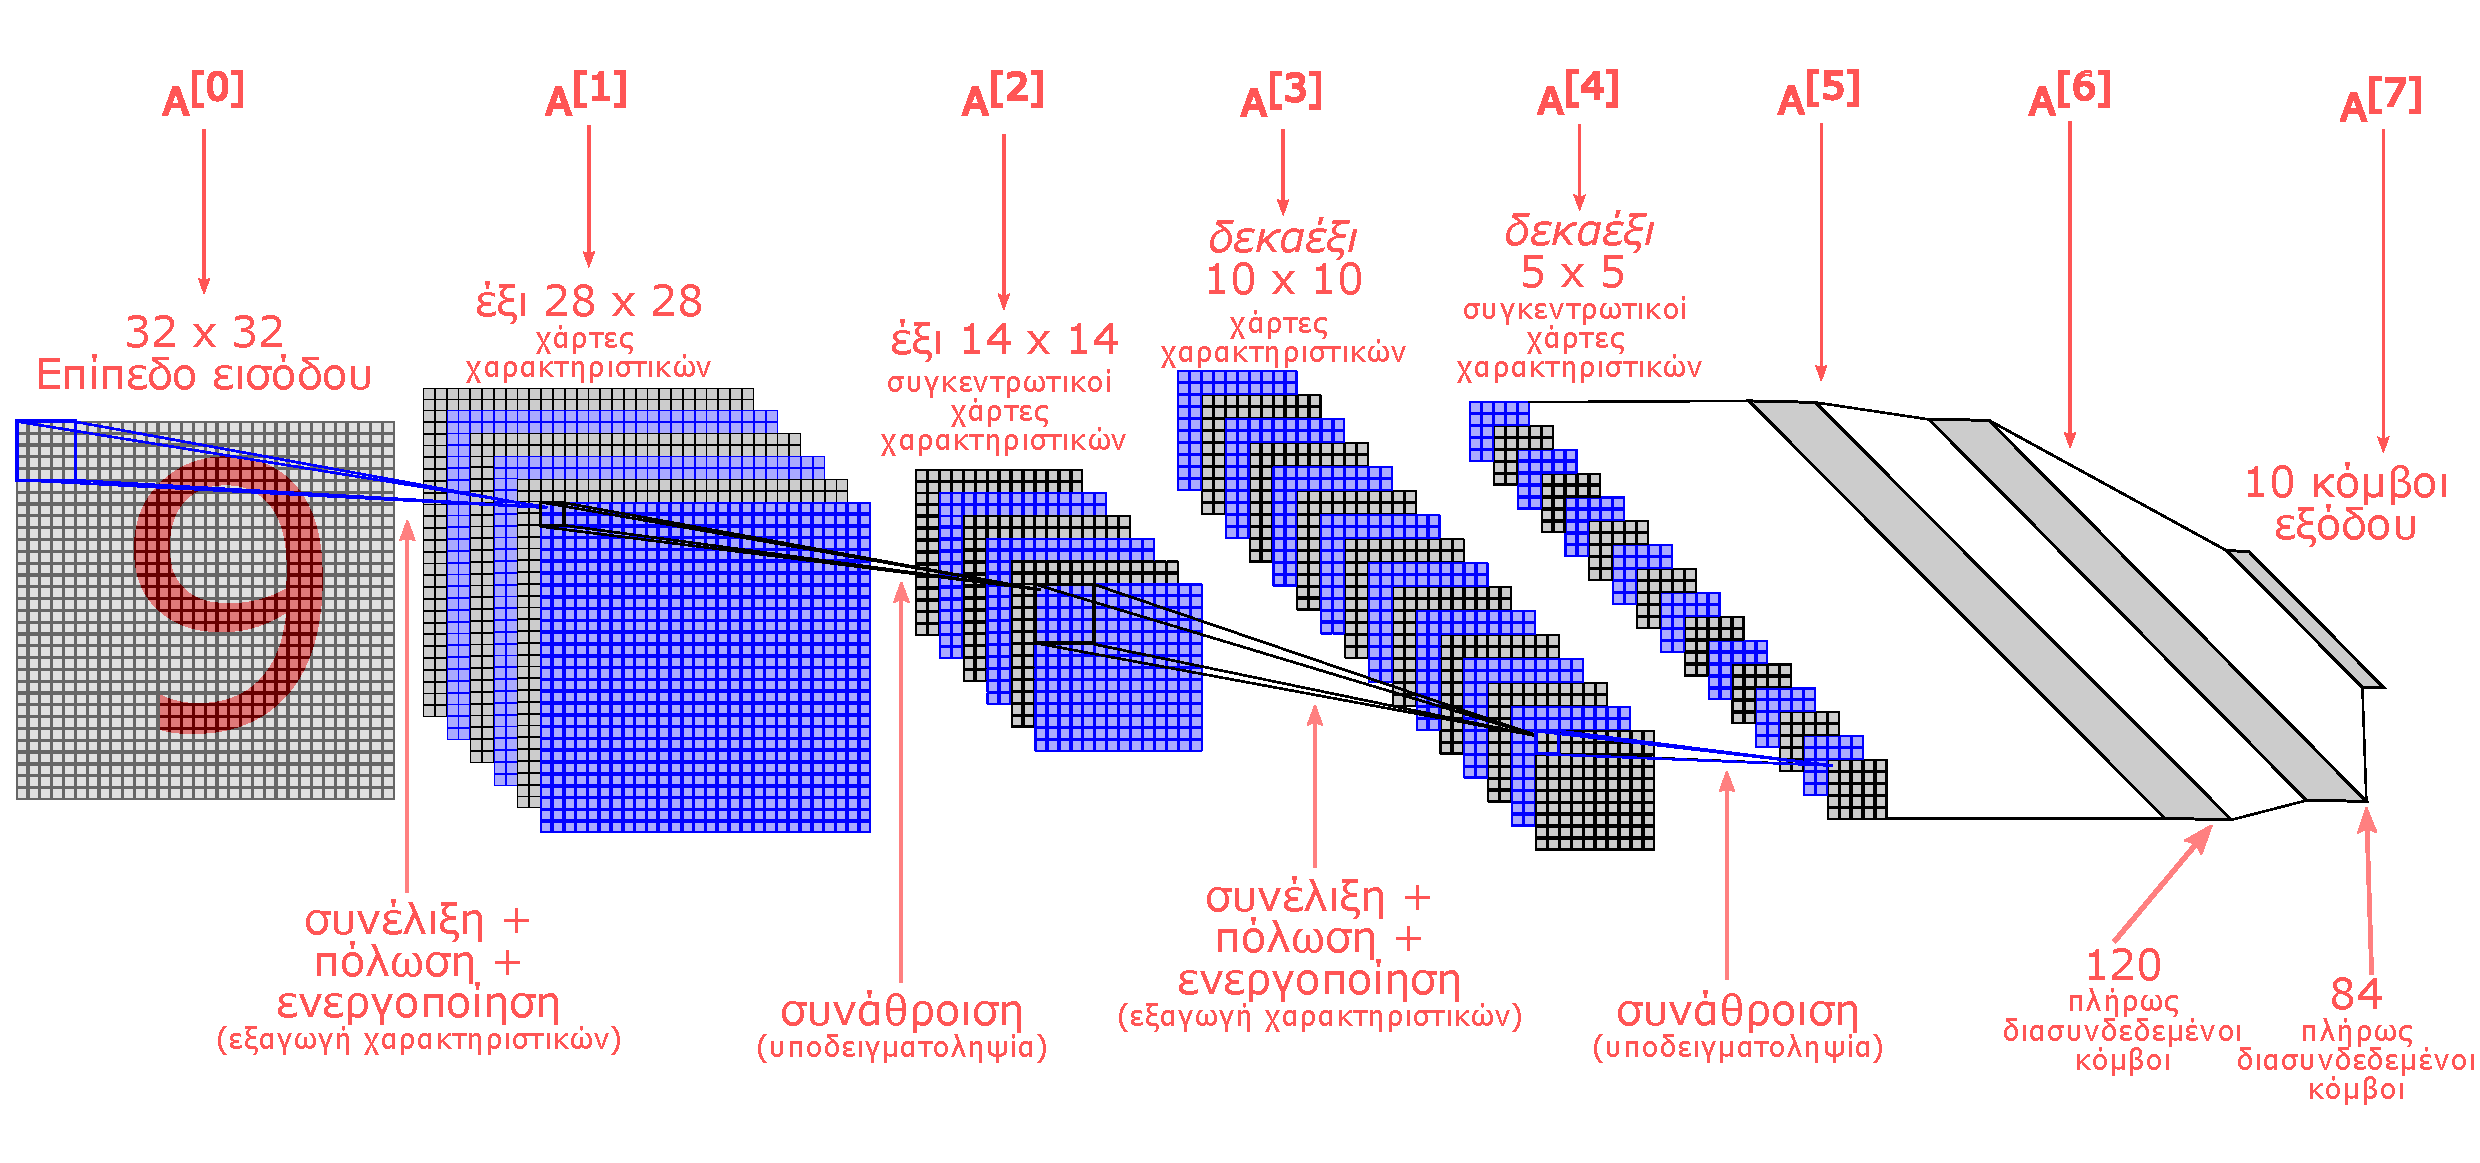
\includegraphics[width=0.95\textwidth]{images/chapter theoritical background/LeNet_good_greek.pdf}
  \caption{Αρχιτεκτονική Συνελικτικού Νευρωνικού Δικτύου (\en{LeNet-5}) \cite{lenet}. Η αναπαράστασή τους διααφέρει από αυτήν των απλών νευρωνικών δικτύων αφού εδώ δίνεται έμφαση στους πίνακες τιμών ενεργοποίησης $A^{[l]}$. Οι χάρτες χαρακτηριστικών αναπαριστώνται με τετράγωνα ενώ τα βάρη με ακμές. Τα δύο τελευταία επίπεδα είναι πλήρως διασυνδεδεμένα. \textit{Παράχθηκε από το \href{https://inkscape.org/}{\en{Inkscape}} τροποποιώντας \href{https://pabloinsente.github.io/the-convolutional-network}{αυτήν την εικόνα}.}}
  \label{fig:_nn_lenet}
\end{figure}

Η λύση στο πρόβλημα δόθηκε μέσω της αξιοποίησης της τοπικής χωρικής συνεκτικότητας (\en{local spacial coherence}) και της ιεραρχικής δομής (\en{hierarchical structure}) των δεδομένων εικόνων. Εμπνευσμένη από τις ανωτέρω επιστημονικές παρατηρήσεις, ενσωματώθηκε η γνώση του χώρου προβλημάτων με εικόνες στη δομή των νευρωνικών δικτύων οδηγώντας έτσι στη δημιουργία των συνελικτικών νευρωνικών δικτύων (βλ. σχήμα \ref{fig:_nn_lenet}). Οι δομικές διαφορές των συνελικτικών νευρωνικών δικτύων που τους διακρίνουν από τα νευρωνικά δίκτυα που παρουσιάστηκαν στην προηγούμενη ενότητα μπορούν να συνοψιστούν ως εξής:
\begin{itemize}
  \item Μια πρώτη διαφορά που επιλύει το πρόβλημα της απαγορευτικής υπολογιστικής πολυπλοκότητας έγκειται στο τρόπο διασύνδεσης των κόμβων ενός επιπέδου με τους κόμβους του αμέσως προηγούμενου. Αντί να είναι πλήρως διασυνδεδεμένοι με αυτούς του προηγούμενου επιπέδου όπως στην περίπτωση των απλών νευρωνικών δικτύων, ενώνονται με βάρη μόνο με αυτούς που ανήκουν στο λεγόμενο πεδίο υποδοχής. Με άλλα λόγια, κάθε νευρώνας επιπέδου $l$ δέχεται σαν είσοδο ενα διαφορετικό και περιορισμένο τμήμα του πίνακα $A^{[l-1]}$.
 
  \item Στα συνελικτικά νευρωνικά δίκτυα, οι κόμβοι του κάθε επιπέδου είναι οργανωμένοι σε όγκους τριών διαστάσεων με πλάτος, ύψος και βάθος. Με αυτόν τον τρόπο, διατηρείται η τοπική χωρική συνεκτικότητα. Αναλυτικότερα, οι κόμβοι εισόδου, για παράδειγμα, οργανώνονται όπως τα εικονοστοιχεία σε μια εικόνα: το βάθος του επιπέδου αντιστοιχεί στον αριθμό των καναλιών της εικόνας (π.χ. \en{RGB}) ενώ το ύψος και το πλάτος του επιπέδου στο ύψος και πλάτος της εικόνας. Έτσι, το νευρωνικό δίκτυο έχει τη δυνατότητα να αντλήσει εύκολα πληροφορία από μια χωρική γειτονιά της εικόνας (το πεδίο υποδοχής κάποιου νευρώνα) αφού οι αποστάσεις μεταξύ των εικονοστοιχείων διατηρούνται αναλλοίωτες. Αν όμως λαμβάναμε την εικόνα και την αναπτύσσαμε σε μια διάσταση (\en{flatten}) σημιουργόντας ένα μεγάλο διάνυσμα, τότε οι σχετικές αποστάσεις των στοιχείων εισόδου δε θα διατηρούνταν. Ανάλογες παρατηρήσεις ισχύουν και για τα κρυφά επίπεδα. Δηλαδή, και στα επόμενα επίπεδα οι κόμβοι οργανώνονται σε τρισδιάστατες δομές οι οποίες διατηρούν τοπικό χαρακτήρα. Η διαφορά έγκειται στο ότι η τιμή των κόμβων των κρυφών επιπέδων δεν είναι η τιμή του εκάστοτε εικονοστοιχείου στη θέση αυτή. Αντίθετα, είναι η τιμή ενός (σύνθετου) χαρακτηριστικού της περιοχής που έχει υπολογιστεί από την επεξεργασία απλούστερων χαρακτηριστικών προηγούμενων επιπέδων. Σχετικά με την ιδιότητα της ιεραρχικής δομής των εικόνων του πραγματικού κόσμου, αυτή αξιοποιείται μέσω διαδοχικών κρυφών επιπέδων που σταδιακά διευρύνουν το οπτικό πεδίο και συνθέτουν ολοένα και πιο σύνθετα χαρακτηριστικά. Έχει δειχθεί, ότι το σύστημα μαθαίνει να εξάγει μέσω των πρώτων επιπέδων απλά χαρακτηριστικά (π.χ. οριζόντιες και κάθετες ακμές) τα οποία σε επόμενα επίπεδα συνδυάζει για να εξάγει πιο περίπλοκα χαρακτηριστικά \cite{zeiler2014visualizing}. Αφού οι κόμβοι είναι οργανωμένοι σε όγκους, προκύπτει φυσικά ότι το διάνυσμα ενεργοποίησης $A^{[l]}$ του κάθε επιπέδου $l$ που κατασκευάζεται από την έξοδο κάθε κόμβου έχει τη μορφή πίνακα τριών διαστάσεων. Διαισθητικά για τα κρυφά επίπεδα, το ύψος και το πλάτος του διανύσματος ενεργοποίησης κωδικοποιούν αμυδρά τη θέση του χαρακτηριστικού στην εικόνα ενώ το βάθος κωδικοποιεί τα διάφορα χαρακτηριστικά (π.χ. βάθος 1: οριζόντιες ακμές, βάθος δύο: κατακόρυφες ακμές\footnote{Πρακτικά στη διαδικασία εκμάθησης χαρακτηριστικών είναι δύσκολο να εκφράσουμε με σαφήνεια τι αναπαριστά το καθένα.}). Στην περίπτωση των δικτύων που εξετάζουμε, το $A^{[l]}$ λέμε ότι αποτελείται από επίπεδα φύλλα τα οποία στοιβάζονται στη διάσταση $z$ και ονομάζονται χάρτες χαρακτηριστικών (\en{feature maps}).
  
  \item Μια ακόμα δομική διαφορά είναι ότι στα συνελικτικά νευρωνικά δίκτυα η εκμάθηση και εξαγωγή των χαρακτηριστικών δε γίνεται ανεξάρτητα σε κάθε περιοχή της εικόνας. Νευρώνες των οποίων τα βάρη προσαρμόζονται ώστε να αναγνωρίζουν και να εξάγουν γενικά χαρακτηριστικά της εικόνας όπως τα χαρακτηριστικά ακμών θα ήταν ασύμφορο να είχαν εφαρμογή μόνο στο πεδίο υποδοχής τους και όχι σε όλη την εικόνα. Έτσι, οδηγούμαστε στην έννοια του διαμοιρασμού παραμέτρων (\en{weight sharing}). Σύμφωνα με αυτήν την έννοια, αντί οι κόμβοι ενός επιπέδου να είναι διασυνδεδεμένοι με τους κόμβους του προηγούμενου επιπέδου με ξεχωριστά βάρη και δυναμικά πόλωσης, οι παράμετροι αυτές μοιράζονται μεταξύ των κόμβων. Έτσι, οι κόμβοι ενός επιπέδου επιτελούν τον ίδιο γραμμικό συνδυασμό $y = f\Big(\sum_{i = 1}^{n} w_i \times x_i  +  b\Big)$ αλλά με διαφορετικό διάνυσμα εισόδου $X$ που εξαρτάται από το οπτικό πεδίο. Σημειώνουμε δε ότι ο διαμοιρασμός βαρών θα ήταν δύσκολο να εφαρμοστεί στην περίπτωση που η είσοδος αποτελούνταν από δομημένα δεδομένα καθώς αυτά μπορεί να είχαν πλήρως ετερογενή χαρακτηριστικά.
\end{itemize}

\begin{figure}[h]
  \centering
  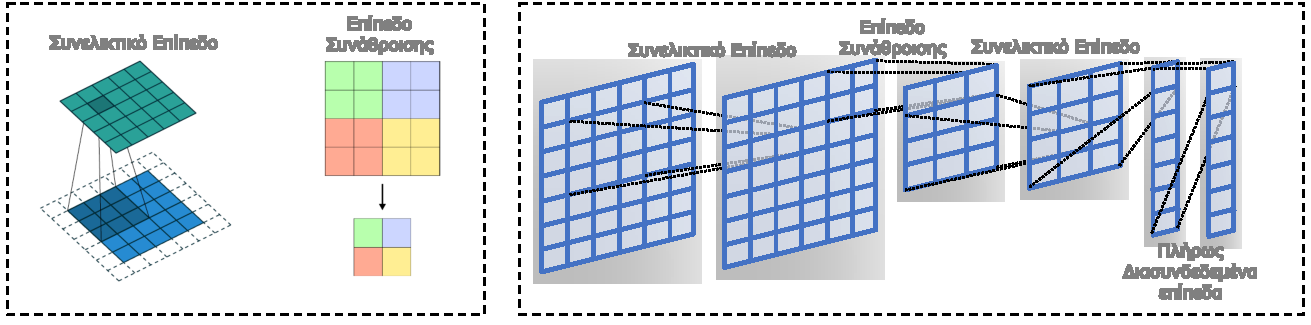
\includegraphics[width=0.9\textwidth]{images/chapter theoritical background/ConvolutionAndPooling_greek.pdf}
  \caption{Μεμονωμένο συνελικτικό επίπεδο και επίπεδο υποδειγματοληψίας (αριστερά). Συνδυασμός των επιπέδων για την κατασκευή ενός συνελικτικού νευρωνικού δικτύου (δεξιά). \textit{Παράχθηκε από το \href{https://inkscape.org/}{\en{Inkscape}} τροποποιώντας \href{https://commons.wikimedia.org/wiki/File:ConvolutionAndPooling.svg}{αυτήν την εικόνα}.}}
  \label{fig:_conv_and_pooling}
\end{figure}

Πρακτικά, αν εξαιρέσουμε τα τελευταία, πλήρως διασυνδεδεμένα επίπεδα ενός συνελικτικού νευρωνικού δικτύου, οι ανωτέρω δομικές διαφορές υλοποιούνται με τη χρήση αφενός των συνελικτικών επιπέδων και αφετέρου των επιπέδων υποδειγματοληψίας. Αναφορικά με τα πρώτα, η εσωτερική τους λειτουργία απεικονίζεται στο αριστερό τμήμα του σχήματος \ref{fig:_conv_and_pooling}.
Το οπτικό πεδίο ανπαρίσταται με ένα σκούρο παραλληλόγραμμο επάνω στον χάρτη χαρακτηριστικών του προηγούμενου επιπέδου. Τα βάρη, είναι ευκολότερο να τα φανταστεί κανείς σαν ένα παραλληλόγραμμο (ή ένα ορθογωνικό κυβοειδές σε τρεις διαστάσεις) το οποίο έχει τις ίδιες διαστάσεις με το οπτικό πεδίο πάνω στο προηγούμενο επίπεδο. Η τιμή ενεργοποίησης κάθε στοιχείου του τρισδιάστατου πίνακα $A^{[l]}$ υπολογίζεται ως το αποτέλεσμα της εφαρμογής της συνάρτησης ενεργοποίησης στον γραμμικό συνδυασμό των στοιχείων του πίνακα $A^{[l-1]}$ που βρίσκονται εντός του οπτικού πεδίου με βάρη τα στοιχεία του $W^{[l]}$ και το δυναμικό πόλωσης $b^{[l]}$. Στην ουσία, τα βάρη υπερτίθενται στο οπτικό πεδίο και επιτελείται γινόμενο μεταξύ των πινάκων στοιχείο προς στοιχείο (\en{elementwise product}). Αν υπήρχε ένας πίνακας από βάρη για κάθε στοιχείο του $A^{[l]}$, τότε δε θα είχαμε διαμοιρασμό βαρών. Αντιθέτως, ο διαμοιρασμός βαρών έγκειται στην ολίσθηση αυτού του παραλληλόγραμμου (ή ορθογωνικού κυβοειδούς στις τρεις διαστάσεις) στο ύψος και πλάτος της εικόνας, όπως φαίνεται και στο σχήμα \ref{fig:_conv2d} για την περίπτωση των δύο διαστάσεων. Για την περίπτωση που έχουμε πολλούς χάρτες χαρακτηριστικών, παραπέμπουμε τον αναγνώστη στο σχήμα \ref{fig:_conv3d}. Αυτή η διαδικασία της ολίσθησης του πίνακα βαρών ονομάζεται δισδιάστατη συνέλιξη\footnote{Τυπικά, η πράξη ονομάζεται διασταυρούμενη συσχέτιση (\en{cross corelation}) και είναι ίδια με τη συνέλιξη αν στην πρώτη περίπτωση αναποδογυρίσουμε τον πυρήνα (γυρνώντας τον ως προς την κύρια και δευτερεύουσα διαγώνιο).}, ενώ το κυλιόμενο παράθυρο ονομάζεται και φίλτρο (\en{filter}) ή πυρήνας (\en{kernel}). \par

\begin{figure}[h]
  \centering
  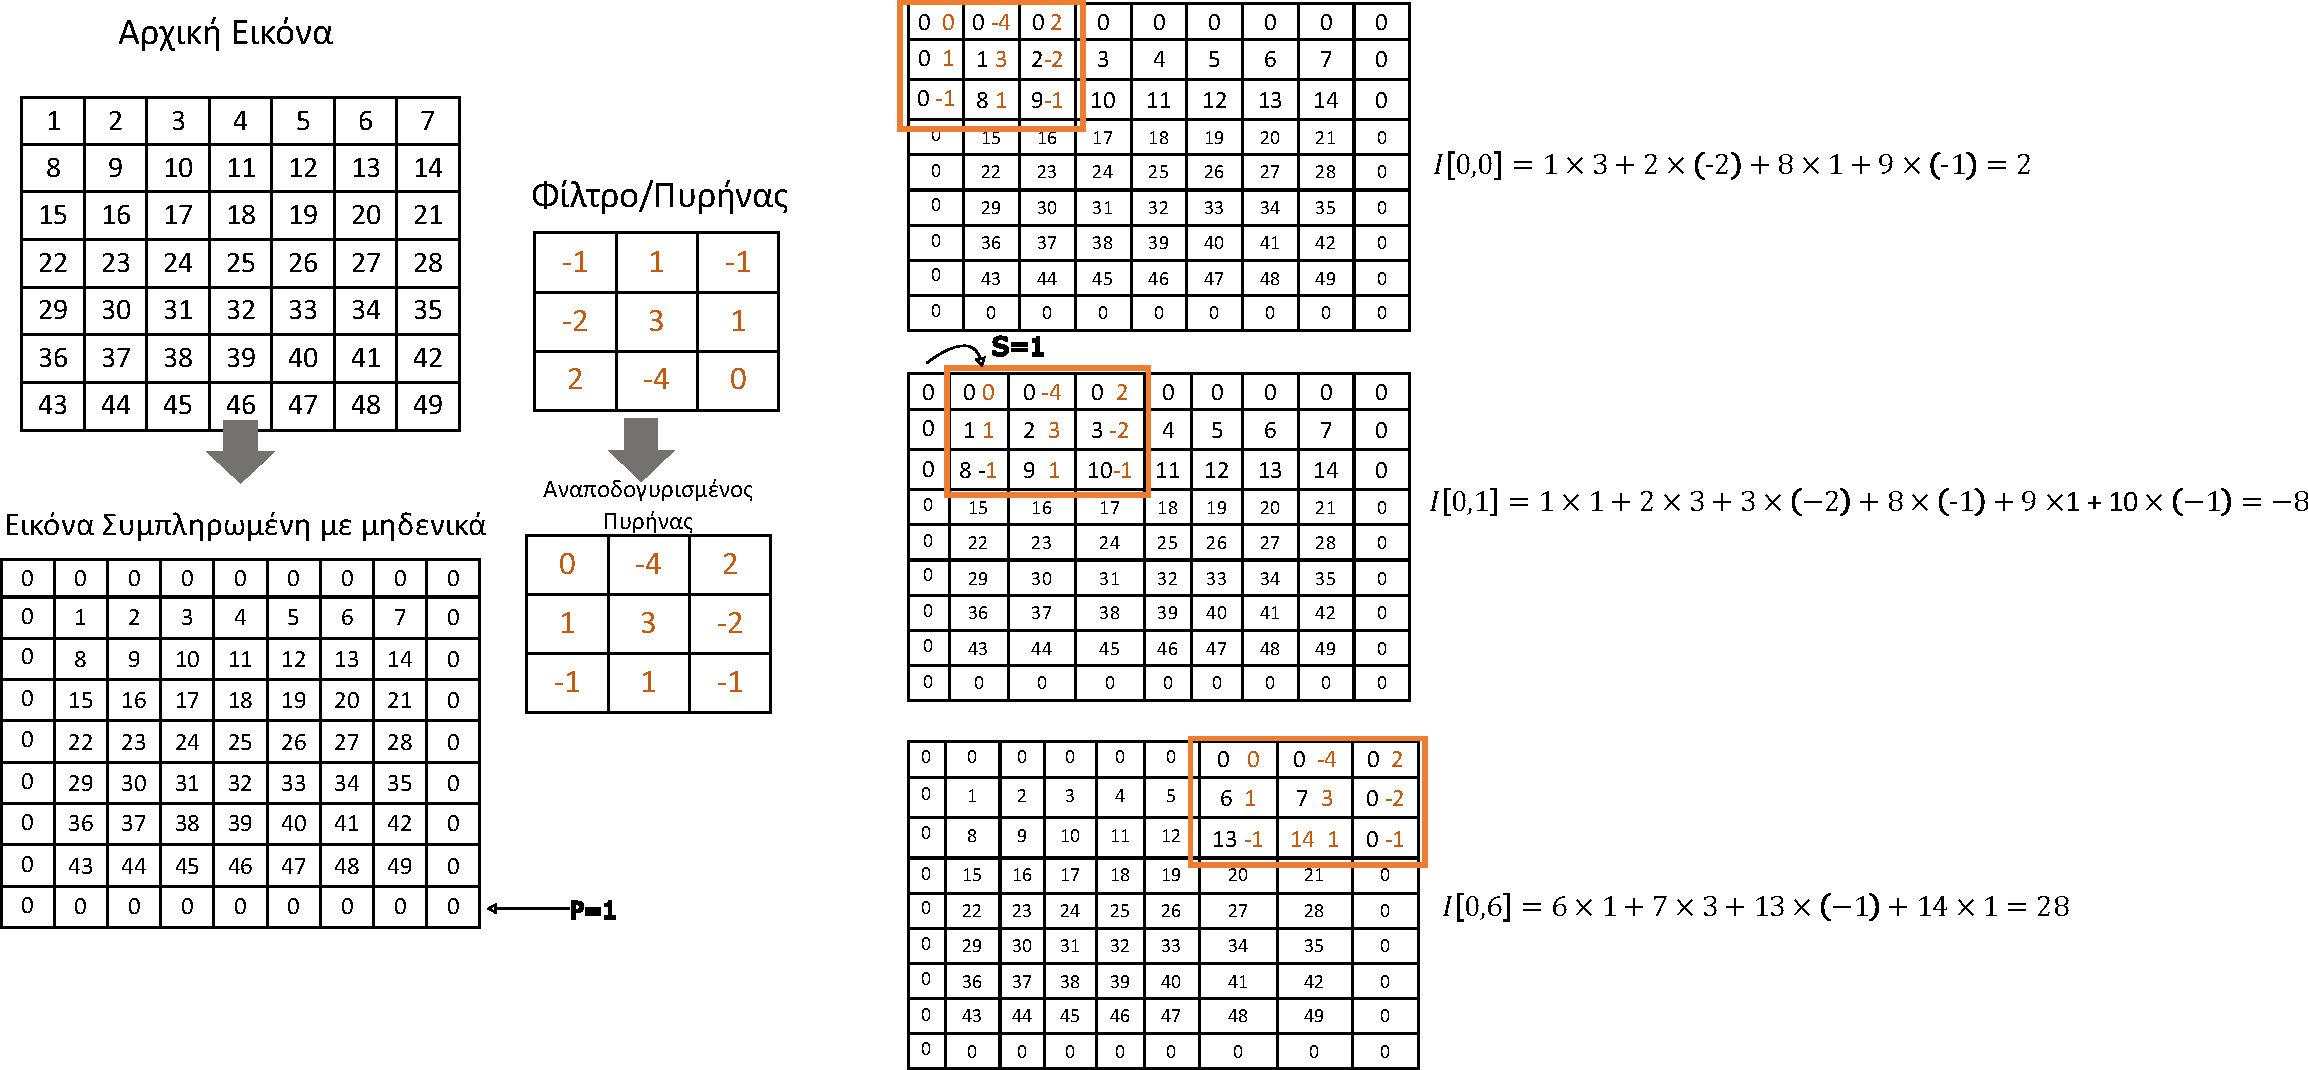
\includegraphics[width=0.9\textwidth]{images/chapter theoritical background/convolve_example_step_1_greek.pdf}
  \caption{Παράδειγμα συνέλιξης σε δύο διαστάσεις \textit{Παράχθηκε από το \href{https://inkscape.org/}{\en{Inkscape}} τροποποιώντας και διορθώνοντας \href{https://empirischtech.at/blog-image-filters}{αυτήν την εικόνα}.}}
  \label{fig:_conv2d}
\end{figure}

Με κάθε συνελικτικό επίπεδο εισάγεται μια σειρά από παραμέτρους πέρα από αυτές που υπήρχαν σε κάθε απλό νευρωνικό δίκτυο. Για κάθε επίπεδο $l$, μεταξύ δύο στοιβαγμένων συνόλων από χάρτες χαρακτηριστικών $A^{[l-1]}$ και $A^{[l]}$ με διαστάσεις ${Width}^{[l-1]} \times {Height}^{[l-1]}\times{Depth}^{[l-1]}$ και ${Width}^{[l]} \times {Height}^{[l]}\times{Depth}^{[l]}$ αντίστοιχα πρέπει να ορίσουμε:
\begin{itemize}
  \item Το μέγεθος του κυλιόμενου πυρήνα (ή φίλτρου). Αυτό εισαγάγει τις παραμέτρους ${F_x}^{[l]}$ και ${F_y}^{[l]}$. Το βάθος του φίλτρου δεν αποτελεί υπερπαράμετρο και είναι ίσο με ${Depth}^{[l-1]}$.
  \item Ο αριθμός των φίλτρων, $K^{[l]}$. Όπως έχει γίνει σαφές από τα ανωτέρω σχήματα, το κάθε φίλτρο $k \in [1,K^{[l]}]$ λαμβάνει σαν είσοδο έναν όγκο από χαρακτηριστικά και έχει ως έξοδο έναν αριθμό $a \in \Re$. Για να έχει ο παραγόμενος χάρτης χαρακτηριστικών βάθος, θα πρέπει να γίνει χρήση πολλαπλών φίλτρων που θα εξάγουν διαφορετικά χαρακτηριστικά. Έτσι, μπορούμε να καθορίσουμε το $ {Depth}^{[l]}$ θέτοντας το $K^{[l]}$ αφού ισχύει ότι $K^{[l]} = {Depth}^{[l]}$. Για κάθε ένα φίλτρο παράγεται ένας χάρτης χαρακτηριστικών.
  \item Το βήμα της συνέλιξης, $s^{[l]}_x$ κατά τον $x$ άξονα και $s^{[l]}_y$ κατά τον $y$ άξονα (συνήθως, οι δύο ποσότητες είναι ίσες και συμβολίζονται ως $s^{[l]}$). Αυτή η ποσότητα καθορίζει το βήμα της ολίσθησης του φίλτρου πάνω στο χάρτη χαρακτηριστικών του επιπέδου $l-1$. Για παράδειγμα, μετά την εφαρμογή του στο άνω αριστερά άκρο της εισόδου στο σχήμα \ref{fig:_conv2d} θα μετακινηθεί με βήμα 1 μια θέση δεξιά (ή κάτω, αργότερα) για να υπολογίσει την επόμενη έξοδο. Στην περίπτωση που η τιμή του βήματος είναι ίση με το μέγεθος του φίλτρου (στον $x$ ή $y$ άξονα), τότε δεν υπάρχει επικάλυψη μεταξύ των οπτικών πεδίων. Μεγαλύτερη τιμή από αυτή δεν είναι επιθυμητή καθώς οδηγεί σε συστηματική αγνόηση στοιχείων του $A^{[l-1]}$.
  \item Το ποσό της περιμετρικής συμπλήρωσης της εισόδου $A^{[l-1]}$ με μηδενικά\footnote{Υπάρχουν και άλλες επιλογές στον τρόπο περιμετρικής συμπλήρωσης όπως αυτός που περιλαμβάνει ανάκλαση αλλά η χρήση μηδενικών είναι η πιο συνηθισμένη μέθοδος και για αυτό εστιάζουμε σε αυτή.}, $P^{[l]}_x$ και $P^{[l]}_y$.  Αν και κάτι τέτοιο δεν είναι απαραίτητο, συνήθως γίνεται για τον έλεγχο των διαστάσεων ύψους και πλάτους του χάρτη χαρακτηριστικών της εξόδου (ή των χαρτών χαρακτηριστικών της εξόδου αν $K^{[l]} > 1$). Μετά από αυτήν τη διαδικασία, καταλήγουμε με ένα σύνολο χαρτών χαρακτηριστικών $\grave{A}^{[l-1]}$ του οποίου οι νέες διαστάσεις είναι $\grave{Width}^{[l-1]} = {Width}^{[l-1]} + 2\times P^{[l]}$ και $\grave{Height}^{[l-1]} = {Height}^{[l-1]} + 2\times P^{[l]}$
\end{itemize}
\begin{figure}[h] 
  \centering
  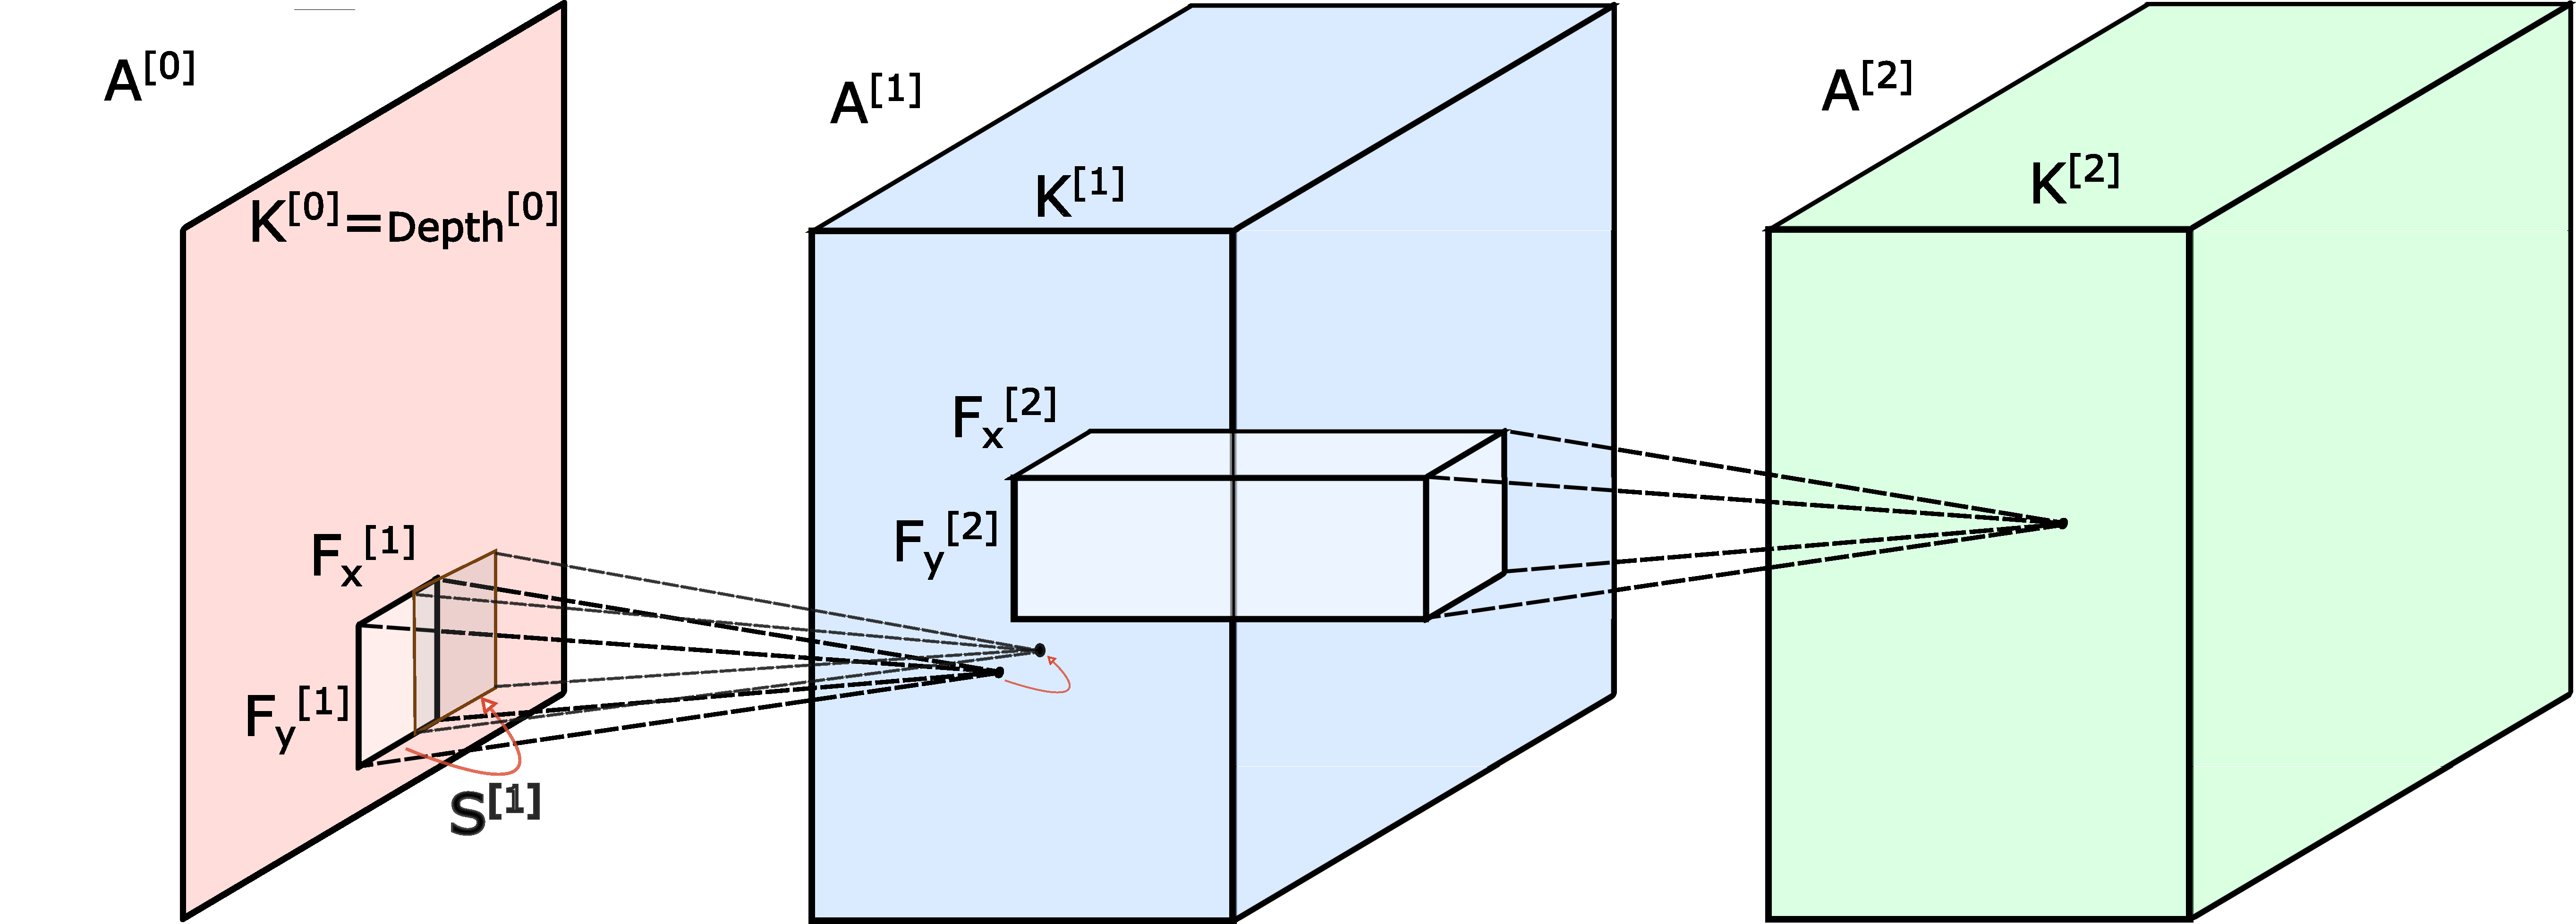
\includegraphics[width=0.9\textwidth]{images/chapter theoritical background/Convolutional_Layers_of_a_Convolutional_Neural_Network.pdf}
  \caption{Συνελικτικά επίπεδα στη σειρά με έμφαση στην περίπτωση όπου οι πίνακες $A$ είναι τριών διαστάσεων. Στο σχήμα φαίνονται οι υπερπαράμετροι των συνελικτικών επιπέδων. \textit{Παράχθηκε από το \href{https://inkscape.org/}{\en{Inkscape}} τροποποιώντας \href{https://commons.wikimedia.org/wiki/File:Convolutional_Layers_of_a_Convolutional_Neural_Network.svg}{αυτήν την εικόνα}.}}
  \label{fig:_conv3d}
\end{figure}
Συγκεντρωτικά, το συνελικτικό επίπεδο, για την παραγωγή ενός συνόλου χαρτών χαρακτηριστικών εφαρμόζει τις εξής διαδικασίες:
\begin{enumerate}
  \item Συνέλιξη πάνω στους χάρτες χαρακτηριστικών $\grave{A}^{[l-1]}$ (αφού έχουν ίσως συμπληρωθεί με μηδενικά) με τον (τρισδιάστατο) πίνακα βαρών $W^{[l]}_k$.
  \item Σημειακή πρόσθεση της τιμής πόλωσης ($b^{[l]}_k$) σε κάθε στοιχείο του προηγούμενου πίνακα με αποτέλεσμα την παραγωγή ενός πίνακα $Z^{[l]}_k$ με τις ίδιες διαστάσεις.
  \item Εφαρμογή συνάρτησης ενεργοποίησης $F^{[l]}$ σημειακά ώστε τελικά να παραχθεί ο χάρτης χαρακτηριστικών $A^{[l]}_k$ με διαστάσεις ίδιες με τον $Z^{[l]}_k$, δηλαδή: 
  \begin{equation}
  {Width}^{[l]}= \frac{{Width}^{[l-1]}-{F_x}^{[l]}+2\times P^{[l]}_x}{S^{[l]}} + 1,
  \end{equation}
  και
  \begin{equation}
    {Height}^{[l]}=\frac{{Height}^{[l-1]}-{F_y}^{[l]}+2\times P^{[l]}_y}{S^{[l]}} + 1
  \end{equation}
  \item Επανάληψη από το βήμα 1 $K^{[l]}$ φορές, όσο και το βάθος του $A^{[l]}$.
  \item Στοίβαξη των παραχθέντων χαρτών χαρακτηριστικών ως προς τον άξονα $z$ ώστε να κατασκευαστεί ο τρισδιάστατος πίνακας $A^{[l]}$. Τελικά, το σύνολο των χαρτών χαρακτηριστικών $A^{[l]}$ έχει διαστάσεις μήκους και πλάτους ίδιες με αυτές του $A^{[l]}_k$ αλλά το βάθος τώρα, αντί για μονάδα είναι:
  \begin{equation}
    {Depth}^{[l]}=K^{[l]}
  \end{equation}
\end{enumerate}
Με μαθηματικούς όρους, οι υπολογισμοί που εκτελούνται σε ένα συνελικτικό επίπεδο είναι οι εξής:
\begin{equation}
  Z^{[l]}_k = {{W^{[l]}_k}^T }^{\tau} \underset{{step=S^{[l]}}} {\ast} A^{[l-1]} + b^{[l]}_k
\end{equation}
και
\begin{equation}
  A^{[l]}_k = F^{[l]}(Z^{[l]}_k).
\end{equation}
Όπου το σύμβολο $\tau$ στον εκθέτη ενός πίνακα δηλώνει την αναστροφή του πίνακα υπό τη δευτερεύουσα διαγώνιο ενώ το σύμβολο $\underset{{step=S^{[l]}}} {\ast}$ δηλώνει τη συνέλιξη με βήμα ίσο με $S^{[l]}$. \par

\begin{figure}[h]
  \centering
  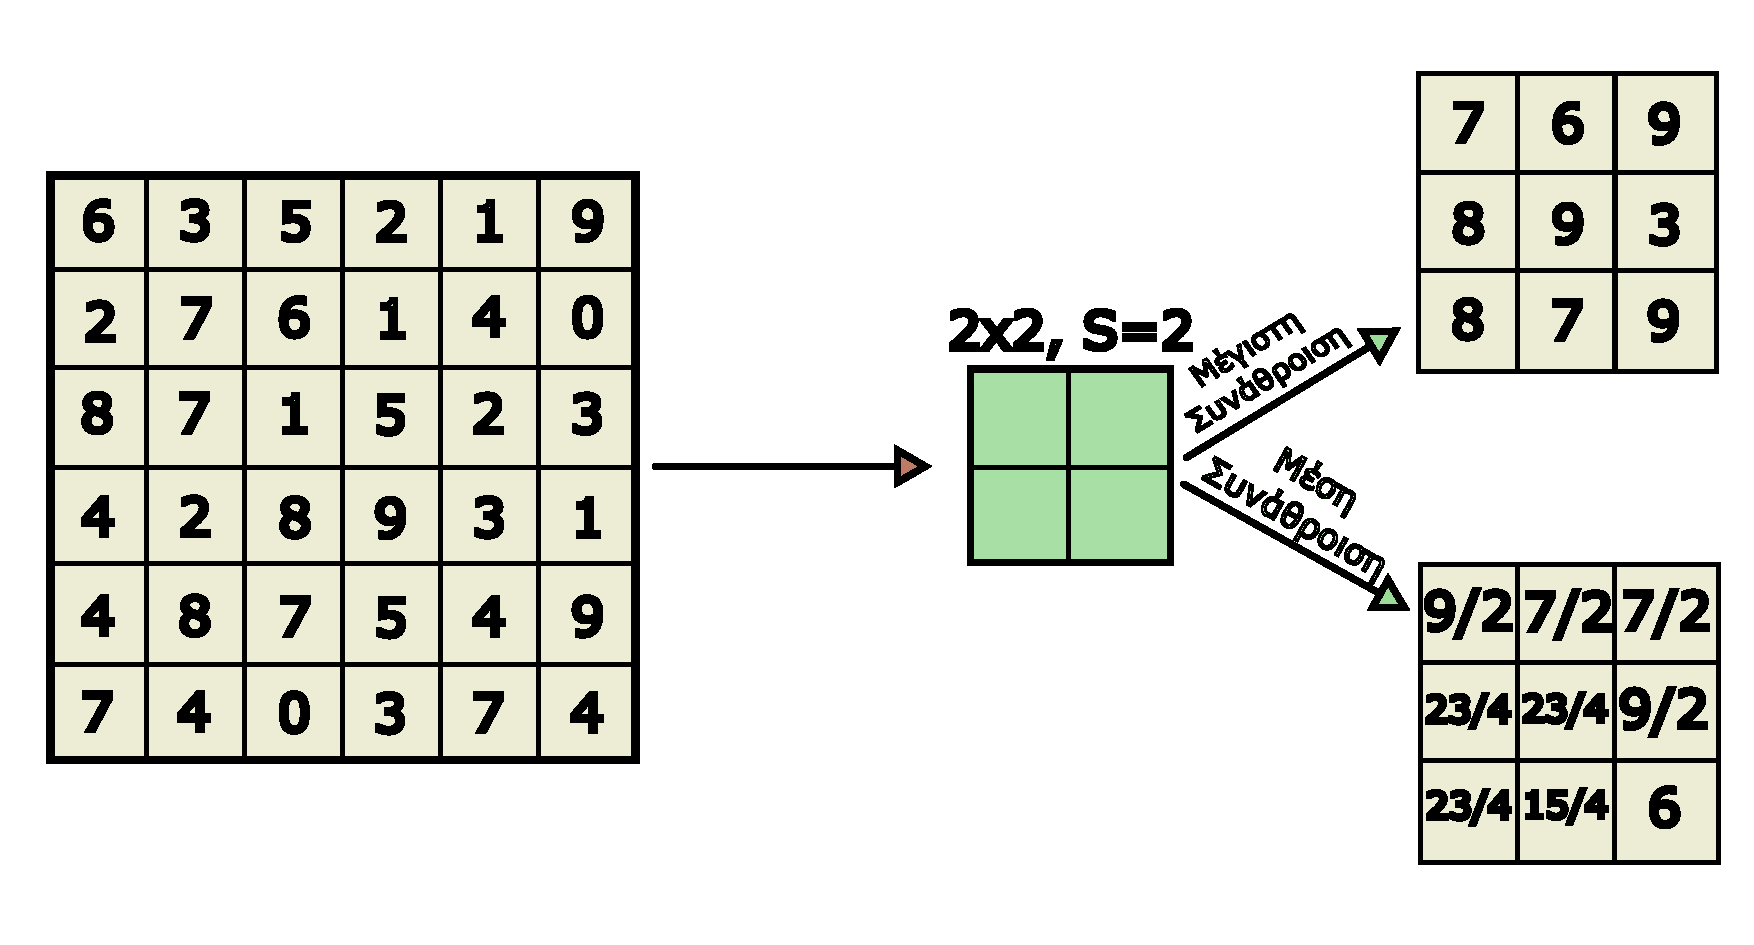
\includegraphics[width=0.95\textwidth]{images/chapter theoritical background/max_avg_pooling_gr.pdf}
  \caption{Σχήμα επιπέδου συνάθροισης. \textit{Παράχθηκε από το \href{https://inkscape.org/}{\en{Inkscape}}.}} 
  \label{fig:max_avg_pooling}
\end{figure}
 
Ένα δεύτερο είδος επιπέδου αποτελεί αυτό της υποδειγματοληψίας (ή συνάθροισης) όπως φαίνεται στο σχήμα \ref{fig:max_avg_pooling}. Το συγκεκριμένο είδος δε διαθέτει καμία παράμετρο αφού η μόνη λειτουργία του είναι να πραγματοποιεί υποδειγματοληψία στο χάρτη χαρακτηριστικών. Ο τρόπος εφαρμογής του είναι παρόμοιος με αυτόν του συνελικτικού επιπέδου. Δηλαδή, και πάλι υπάρχει ένα κυλιόμενο παράθυρο πάνω στον χάρτη χαρακτηριστικών το οποίο συναθροίζει τα στοιχεία στα οποία υπερτίθεται σε ένα στοιχείο υπό μια προκαθορισμένη στρατηγική. Πιο συγκεκριμένα, ανάλογα με το αν επιλέγεται σαν έξοδος το μεγαλύτερο στοιχείο στη γειτονιά συνάθροισης (το οπτικό πεδίο) ή μια μέση τιμή αυτών, έχουμε τη μέγιστη συνάθροιση (\en{max pooling}) ή τη μέση συνάθροιση (\en{average pooling}) αντίστοιχα. Σε κάθε περίπτωση, μια διαφορά με τα συνελικτικά επίπεδα είναι ότι το κυλιόμενο παράθυρο υπερτίθεται σε κάθε \textquote{φύλλο} της εισόδου $A^{[l-1]}$ ξεχωριστά (δηλαδή, σε κάθε $A^{[l-1]}_k$). Με άλλα λόγια, παρόλο που ο πίνακας $A^{[l-1]}$ μπορεί να είναι τρισδιάστατος και να αποτελείται από πολλούς χάρτες χαρακτηριστικών στοιβαγμένους στον $z$ άξονα, η γειτονιά συνάθροισης θα είναι πάντα ένα δισδιάστατο παράθυρο. Τέλος, να σημειώσουμε ότι αυτό το επίπεδο συμβάλλει στην ευρωστία του συστήματος καθιστώντας τις τιμές ενεργοποίησης των επόμενων επιπέδων αμετάβλητες σε μικρές διακυμάνσεις της θέσης των αντικειμένων, μια ιδιότητα που θα αναλύσουμε περαιτέρω στην επόμενη ενότητα. \par

Σε κάθε επίπεδο συνάθροισης $l$ έχουμε τις εξής υπερπαραμέτρους:
\begin{itemize}
  \item Το μέγεθος του πυρήνα υποδειγματοληψίας ${Pk_x}^{[l]}$ και ${Pk_y}^{[l]}$. Καθορίζει τη γειτονιά συνάθροισης αλλά και το μέγεθος του συναθροισμένου χάρτη χαρακτηριστικών.
  \item Τη στρατιγική του επιπέδου συνάθροισης. Όπως αναφέραμε, εδώ οι στρατηγικές είναι δύο: μέγιστη συνάθροιση και μέση συνάθροιση.
  \item Το βηματισμό του κυλιόμενου παραθύρου $s^{[l]}_x$ κατά τον $x$ άξονα και $s^{[l]}_y$ κατά τον $y$ άξονα (όπως και στα συνελικτικά επίπεδα, συνήθως, οι δύο ποσότητες είναι ίσες και συμβολίζονται ως $s^{[l]}$). Ήθιστε, το βήμα να ισούται με το μέγεθος του πυρήνα.
\end{itemize}

Αναφορικά με το μέγεθος της εξόδου ενός επιπέδου συνάθροισης $l$, με είσοδο έναν χάρτη χαρακτηριστικών $A^{[l-1]}$ με διαστάσεις ${Width}^{[l-1]} \times {Height}^{[l-1]}\times{Depth}^{[l-1]}$ ισχύει:
\begin{equation}
  {Width}^{[l]}= \frac{{Width}^{[l-1]}-{Pk_x}^{[l]}}{S^{[l]}} + 1,
  \end{equation}
  \begin{equation}
    {Height}^{[l]}=\frac{{Height}^{[l-1]}-{Pk_y}^{[l]}}{S^{[l]}} + 1
  \end{equation}
  και
  \begin{equation}
    {Depth}^{[l]}={Depth}^{[l-1]}
  \end{equation}

Έχοντας καλύψει πλήρως τα νευρωνικά δίκτυα και την υποκατηγορία τους η οποία χρησιμοποιείται στην όραση υπολογιστών, είμαστε σε θέση να περιγράψουμε ένα νεότερο είδος νευρωνικών δικτύων για τον ίδιο σκοπό, τα λεγόμενα νευρωνικά δίκτυα με κάψουλες.

% \subsubsection{Στρατηγικές Βελτίωσης Απόδοσης Νευρωνικών Δικτύων}

\section{Νευρωνικά Δίκτυα με Κάψουλες}
Τα τελευταία χρόνια, διερευνάται μια ακόμα παραλλαγή των νευρωνικών δικτύων για εφαρμογές όρασης υπολογιστών: αυτή των νευρωνικών δικτύων με κάψουλες (\en{capsule networks}). Η ιδέα πίσω από τη νέα αρχιτεκτονική παρουσιάστηκε από τον \en{Geoffrey Hinton}, το ίδιο άτομο που είχε συμβάλει καθοριστικά στην ανάπτυξη και εδραίωση των συνελικτικών δικτύων \cite{krizhevsky2012imagenet}. Αυτή τη φορά όμως, στα σχετικά έργα του \cite{kosiorek2019stacked, sabour2017dynamic, hinton2018matrix} τονίζει ορισμένες αδυναμίες της εδραιωμένης, πλέον, τεχνολογίας ενώ προτείνει μια νέα αρχιτεκτονική που θα τις αντιμετωπίζει. Ένας έμπειρος αναγνώστης μπορεί να επισημάνει ότι η σύλληψη της ιδέας των νευρωνικών δικτύων με κάψουλες δεν είναι νέα (2011). Παρόλα αυτά, όπως θα διαπιστώσουμε στο κεφάλαιο \ref{chap:related_work} μόλις πρόσφατα άρχισε να λαμβάνει πρακτική υπόσταση με την ανάπτυξή σύνθετων αρχιτεκτονικών που την πραγματώνουν.\par

Στην ενότητα αυτή θα ξεκινήσουμε κάνοντας αναφορά σε ορισμένα στοιχεία του ανθρώπινου μηχανισμού αναγνώρισης προτύπων εικόνων που αποτέλεσαν πηγή έμπνευσης για τα νευρωνικά δίκτυα με κάψουλες. Έπειτα, θα διατυπώσουμε τα ισχυρά και αδύναμα σημεία που παρουσιάζουν τα συνελικτικά νευρωνικά δίκτυα της προηγούμενης ενότητας. Τέλος, βασιζόμενοι στα κύρια έργα του \en{Geoffrey Hinton} σχετικά με τα νευρωνικά δίκτυα με κάψουλες στο πλαίσιο επιβλεπόμενης μάθησης \cite{kosiorek2019stacked, sabour2017dynamic, hinton2018matrix}, θα εμβαθύνουμε στις αρχές λειτουργίας τους.\par

\subsection{Στοιχεία Έμπνευσης των Νευρωνικών Δικτύων με Κάψουλες}
Για άλλη μια φορά, πηγή έμπνευσης για αυτήν την υποκατηγορία των νευρωνικών δικτύων με την οποία θα ασχοληθούμε σε μεγάλο βαθμό στην υπόλοιπη έκταση της εργασίας αποτέλεσε η νευροφυσιολογία. Πιο αναλυτικά, όπως έχουμε αναφέρει και στην ενότητα \ref{sec:historic_note}, οι νευρώνες στον εγκέφαλο οργανώνονται σε ολοένα και μεγαλύτερες δομές ανάλογα με τη λειτουργία τους. Σε γενικές γραμμές, γειτονικοί νευρώνες που επιτελούν παρόμοιες λειτουργίες ενισχύουν τις μεταξύ τους συνδέσεις σχηματίζοντας συστάδες\footnote{Παράδειγμα συστάδων με νευρώνες στον άνθρωπο που διαθέτουν κοινή είσοδο και κοινή έξοδο είναι η φλοιική μικρή στήλη (\en{cortical minicolumn})}. Προκύπτει λοιπόν η διάθεση πειραματισμού για τη σχεδίαση μιας αρχιτεκτονικής νευρωνικών δικτύων που θα εμπεριέχει ρητά συστάδες από νευρώνες\footnote{Στις μέχρι τώρα αρχιτεκτονικές πλήρως διασυνδεδεμένων νευρωνικών δικτύων που έχουμε παρουσιάσει, δεν υπάρχουν τέτοιες δομές. Θα μπορούσαμε να υποθέσουμε ότι κάθε επίπεδο από νευρώνες αποτελεί μια τέτοια οργανωτική δομή. Η υπόθεση αυτή όμως δεν είναι πλήρως ευσταθής καθότι εσωτερικά αυτής οι νευρώνες δεν αλληλεπιδρούν άμεσα μεταξύ τους.}. Αυτές τις συστάδες θα τις ονομάζουμε και κάψουλες (\en{capsules}).\par

Επιπρόσθετα, έχει παρατηρηθεί ότι ο άνθρωπος αναγνωρίζει ένα αντικείμενο δημιουργώντας δυναμικά ένα ιεραρχικό δέντρο του οποίου η ρίζα εμπεριέχει το αντικείμενο προς αναγνώριση \textemdashυπό μια κωδικοποιημένη αναπαράσταση\textemdash ενώ τα κλαδιά τα επιμέρους τμήματα (ή χαρακτηριστικά) από τα οποία απαρτίζεται. Εκτός αυτού, θα μπορούσαμε να ισχυριστούμε ότι η ιεραρχική δομή είναι \textquote{εμπλουτισμένη}, υπό την έννοια ότι τα κλαδιά του δέντρου κωδικοποιούν τη σχετική θέση των επιμέρους τμημάτων\cite{hinton2021represent}. Αυτό προκύπτει από το γεγονός ότι ο άνθρωπος, με την αναγνώριση ενός αντικειμένου είναι πάντα σε θέση να προσδιορίσει τη σχετική θέση των μερών του (βλ. σχήμα \ref{fig:car}).Η ιεραρχική δομή μεταξύ των αντικειμένων και των αποτελούμενων μερών του φαίνεται να υπάρχει παντού στη φύση. Είναι λογική λοιπόν η επιδίωξη ρητής ενσωμάτωσης μηχανισμών στα νευρωνικά δίκτυα που θα αξιοποιούν την πρότερη γνώση σχετικά με την εμπλουτισμένη ιεραρχική δομή των αντικειμένων του φυσικού κόσμου\footnote{Μπορεί να ισχυριστεί κανείς ότι κάτι τέτοιο ισχύει σε αδρές γραμμές στα κλασσικά είδη βαθιών νευρωνικών δικτύων όπου εξάγοντας απλούστερα χαρακτηριστικά στα πρώτα επίπεδα καθίστανται ικανά να συνθέσουν πιο σύνθετα χαρακτηριστικά στα επόμενα. Μολονότι τα κλασσικά είδη αναλύουν τα δεδομένα μέσω διαδοχικών επιπέδων αξιοποιώντας έτσι την ιεραρχική τους φύση, αδυνατούν εκ'κατασκευής να ενσωματώσουν με ρητό τρόπο τη γνώση των σχέσεων σύνδεσης μεταξύ μερών του όλου (τμημάτων ενός αντικειμένου) και του όλου (ολόκληρου του αντικειμένου).}.\par
\begin{figure}[h]
  \centering
  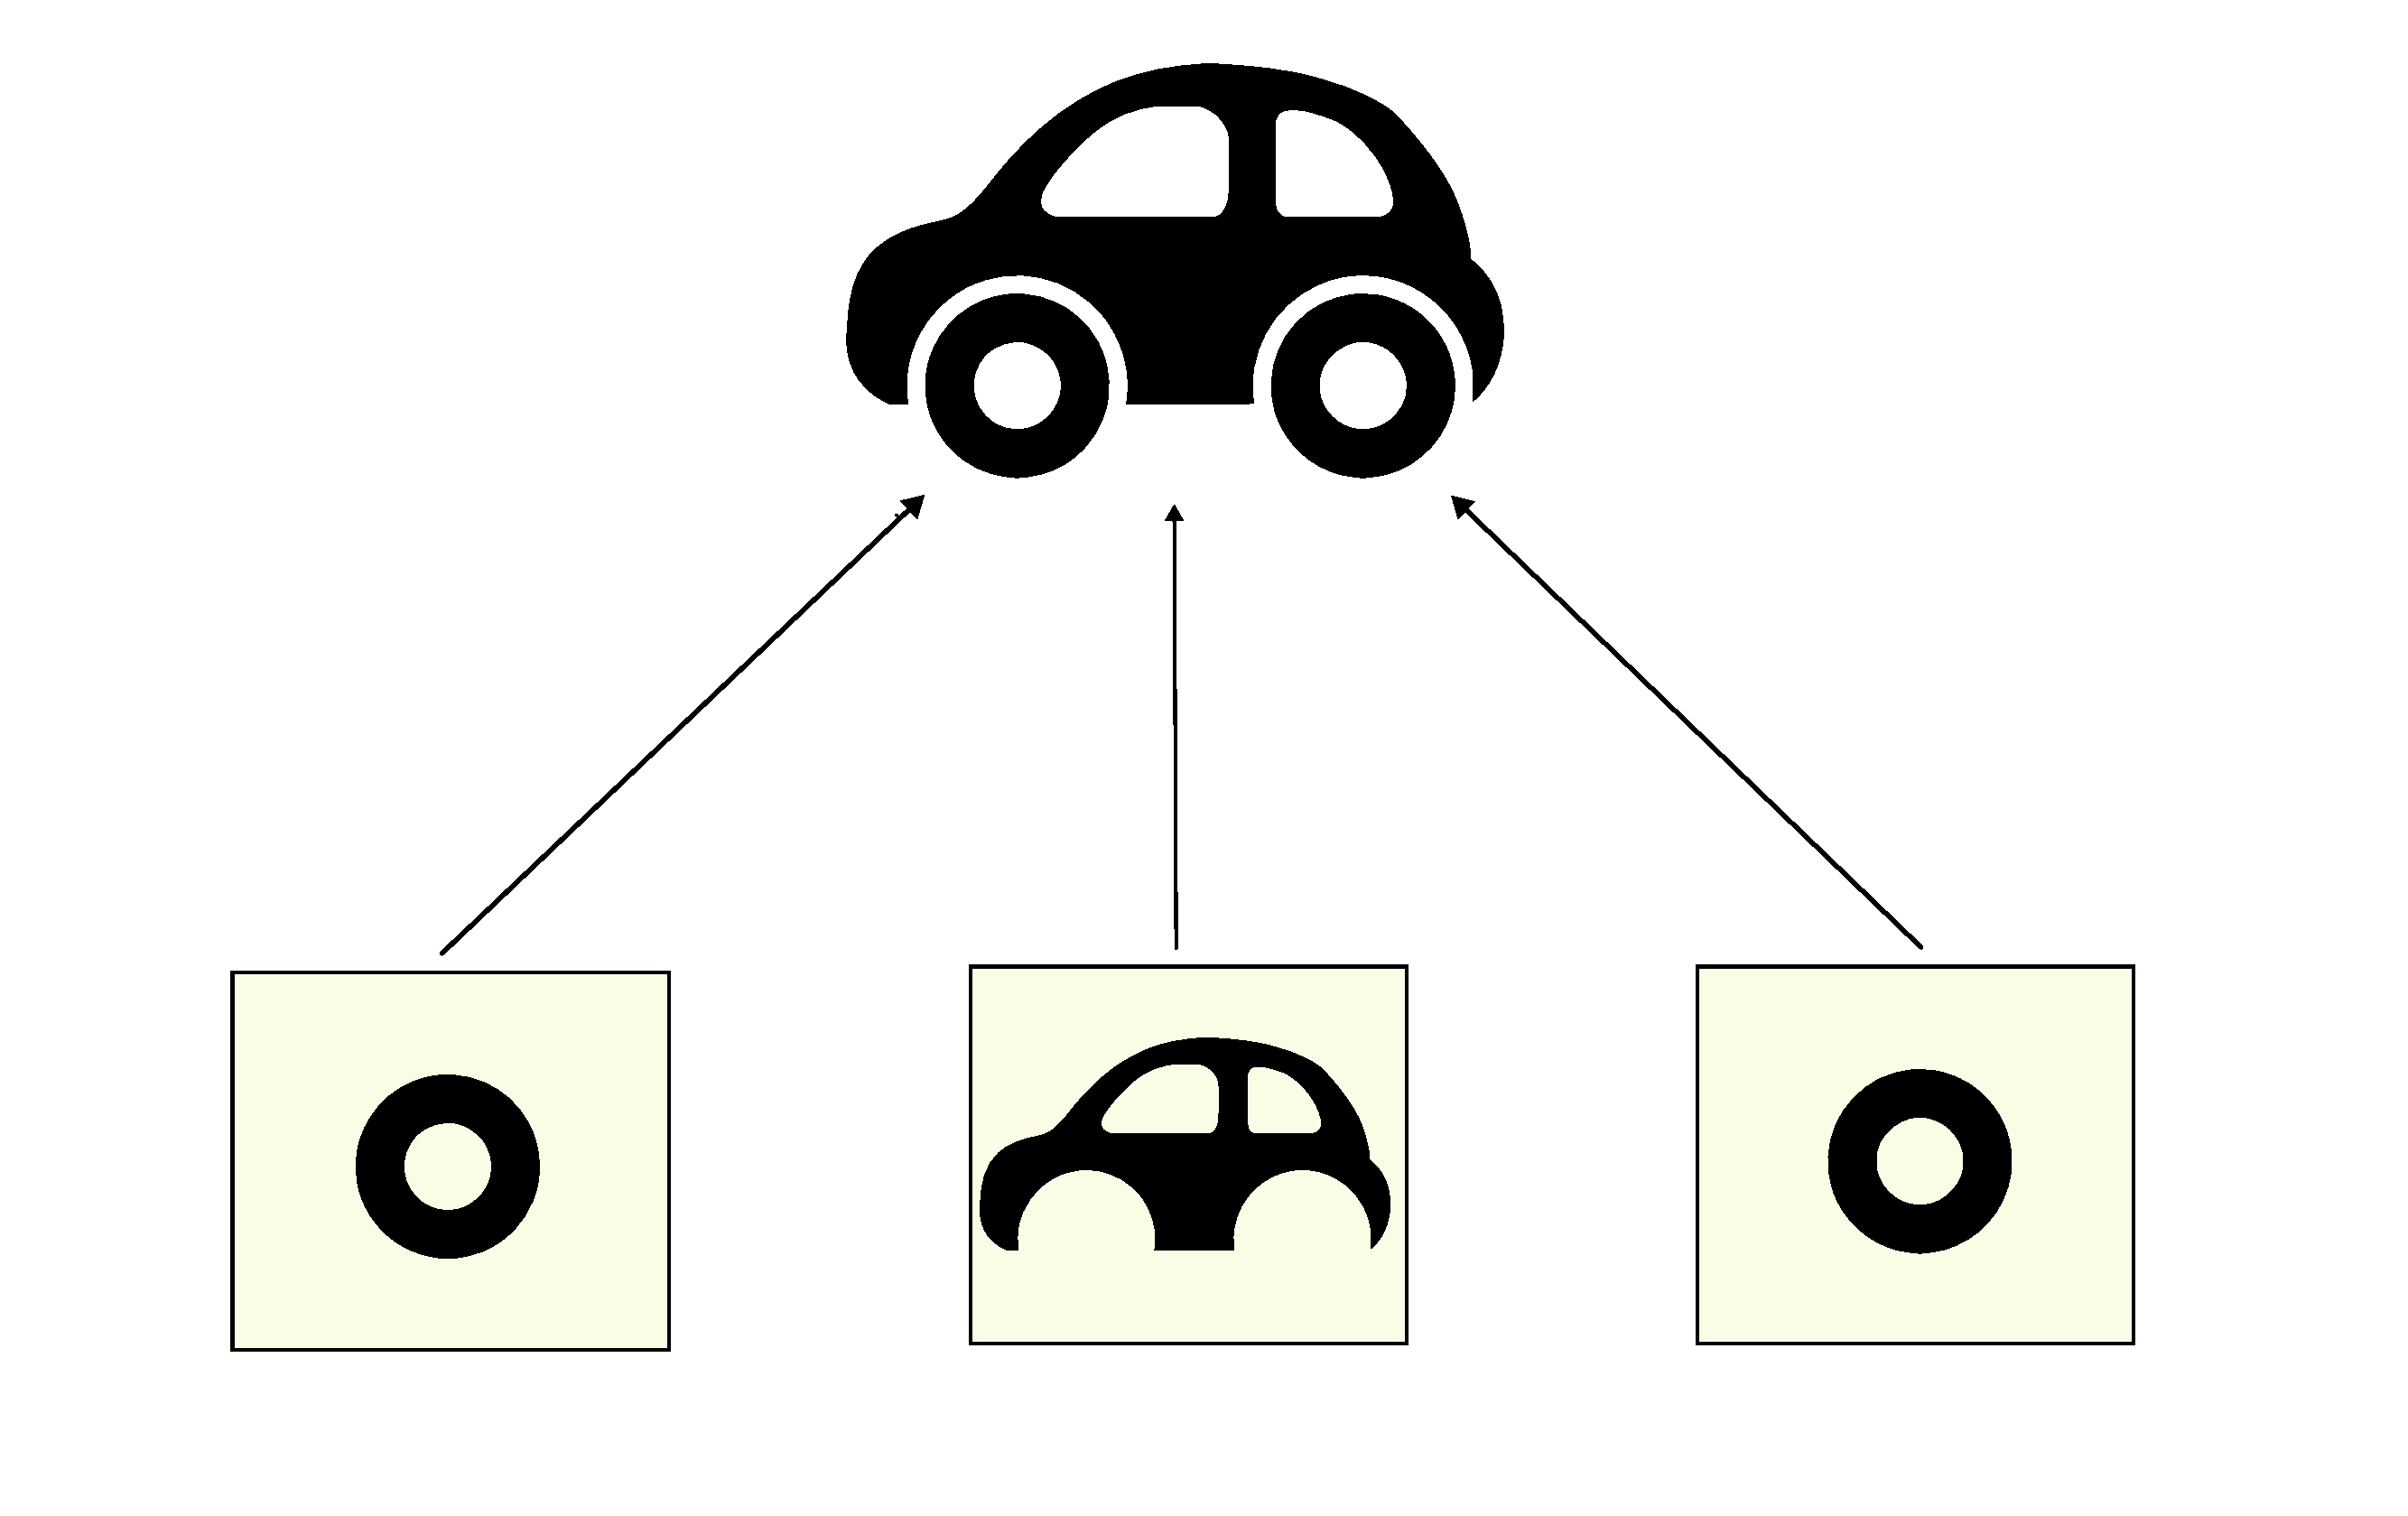
\includegraphics[width=0.7\textwidth]{images/chapter theoritical background/car_tree.pdf}
  \caption{Σχήμα ιεραρχικού δέντρου μιας εικόνας αυτοκινήτου. \textit{Παράχθηκε από το \href{https://inkscape.org/}{\en{Inkscape}}.}} 
  \label{fig:car}
\end{figure} 
Το τρίτο και ίσως πιο σημαντικό στοιχείο από το οποίο εμπνεύστηκαν τα νευρωνικά δίκτυα με κάψουλες προκύπτει από την παρατήρηση ότι οι άνθρωποι πάντα εφαρμόζουν ένα σύστημα συντεταμένων στα αντικείμενα που αναγνωρίζουν. Με άλλα λόγια, η αναγνώριση ενός αντικειμένου είναι άρρηκτα διασυνδεδεμένη με την αναγνώριση της γεωμετρίας του αντικειμένου. Για παράδειγμα, με τη θόραση ενός αυτοκινήτου αντιλαμβανόμαστε άμεσα και τον προσανατολισμό του. Μάλιστα, όπως φαίνεται στο σχήμα \ref{fig:my_wife} ο τρόπος με τον οποίο εφαρμόζεται το σύστημα συντεταγμένων σε μια εικόνα διαδραματίζει πρωτεύοντα ρόλο στην κατανόησή της. Αυτή η λειτουργία του ανθρώπινου οπτικού φλοιού μας προδιαθέτει να δοκιμάσουμε στα τεχνητά νευρωνικά δίκτυα τη ρητή εκμάθηση ενός συστήματος αναφοράς για κάθε αντικείμενο που καλούνται να αναγνωρίσουν και τη σύγκριση κάθε νέας εικόνας εισόδου με αυτό. Όπως θα δούμε στη συνέχεια, μια τέτοια μέθοδος θα οδηγήσει το νευρωνικό δίκτυο σε αποδοτικότερη γενίκευση σχετικά με την εργασία αναγνώρισης αντικειμένων σε νέες γεωμετρίες.

\begin{figure}[h]
  \centering
  
\includegraphics[width=0.25\textwidth]{images/chapter theoritical background/My_wife_and_my_mother_in_law.pdf}
  \caption{Σχήμα όπου απεικονίζεται μια ηλικιωμένη κυρία και μια νεαρή γυναίκα ταυτόχρονα. Ανάλογα με το πιο σύστημα αναφοράς θεωρούμε (προσανατολισμός του κεφαλιού), ο εγκέφαλός μας κάτω από το ίδιο οπτικό ερέθισμα αναγνωρίζει δύο πρόσωπα. \textit{Εγινε λήψη από \href{https://commons.wikimedia.org/wiki/File:My_Wife_and_My_Mother-In-Law_(Hill).svg}{αυτή την ιστοσελίδα}.}} 
  \label{fig:my_wife}
\end{figure} 

\subsection{Θετικά Γνωρίσματα Συνελικτικών Νευρωνικών Δικτύων}
\label{sec:positives_of_cnns}
Προτού αναφερθούμε στα μειονεκτήματα των συνελικτικών νευρωνικών δικτύων που θέλουμε να βελτιώσουμε με τα νευρωνικά δίκτυα από κάψουλες, κρίνεται σκόπιμο να αναγνωρίσουμε ορισμένα θετικά στοιχεία τους τα οποία είναι χρήσιμο να κρατήσουμε. Τα βασικά θετικά στοιχεία που έχουμε προαναφέρει συνοπτικά είναι:
\begin{itemize}
\item Η αξιοποίηση της χωρικής συνεκτικότητας της εισόδου με τη διατήρηση των σχέσεων απόστασης μεταξύ των χαρακτηριστικών και τη χρήση φίλτρων εξαγωγής χαρακτηριστικών που δρουν τοπικά.
\item Η αξιοποίηση της ιεραρχικής δομής των δεδομένων εικόνων με την ενσωμάτωση διαδοχικών συνελικτικών επιπέδων. Ως εκ'τούτου, τα φίλτρα των βαθύτερων επιπέδων έχουν μεγαλύτερο οπτικό πεδίο και δύνανται να συνθέσουν πιο σύνθετα χαρακτηριστικά κωδικοποιώντας έτσι πληροφορία ευρύτερου τμήματος της εικόνας εισόδου (βλ. σχήμα \ref{fig:fov}).
\begin{figure}[h]
  \centering
  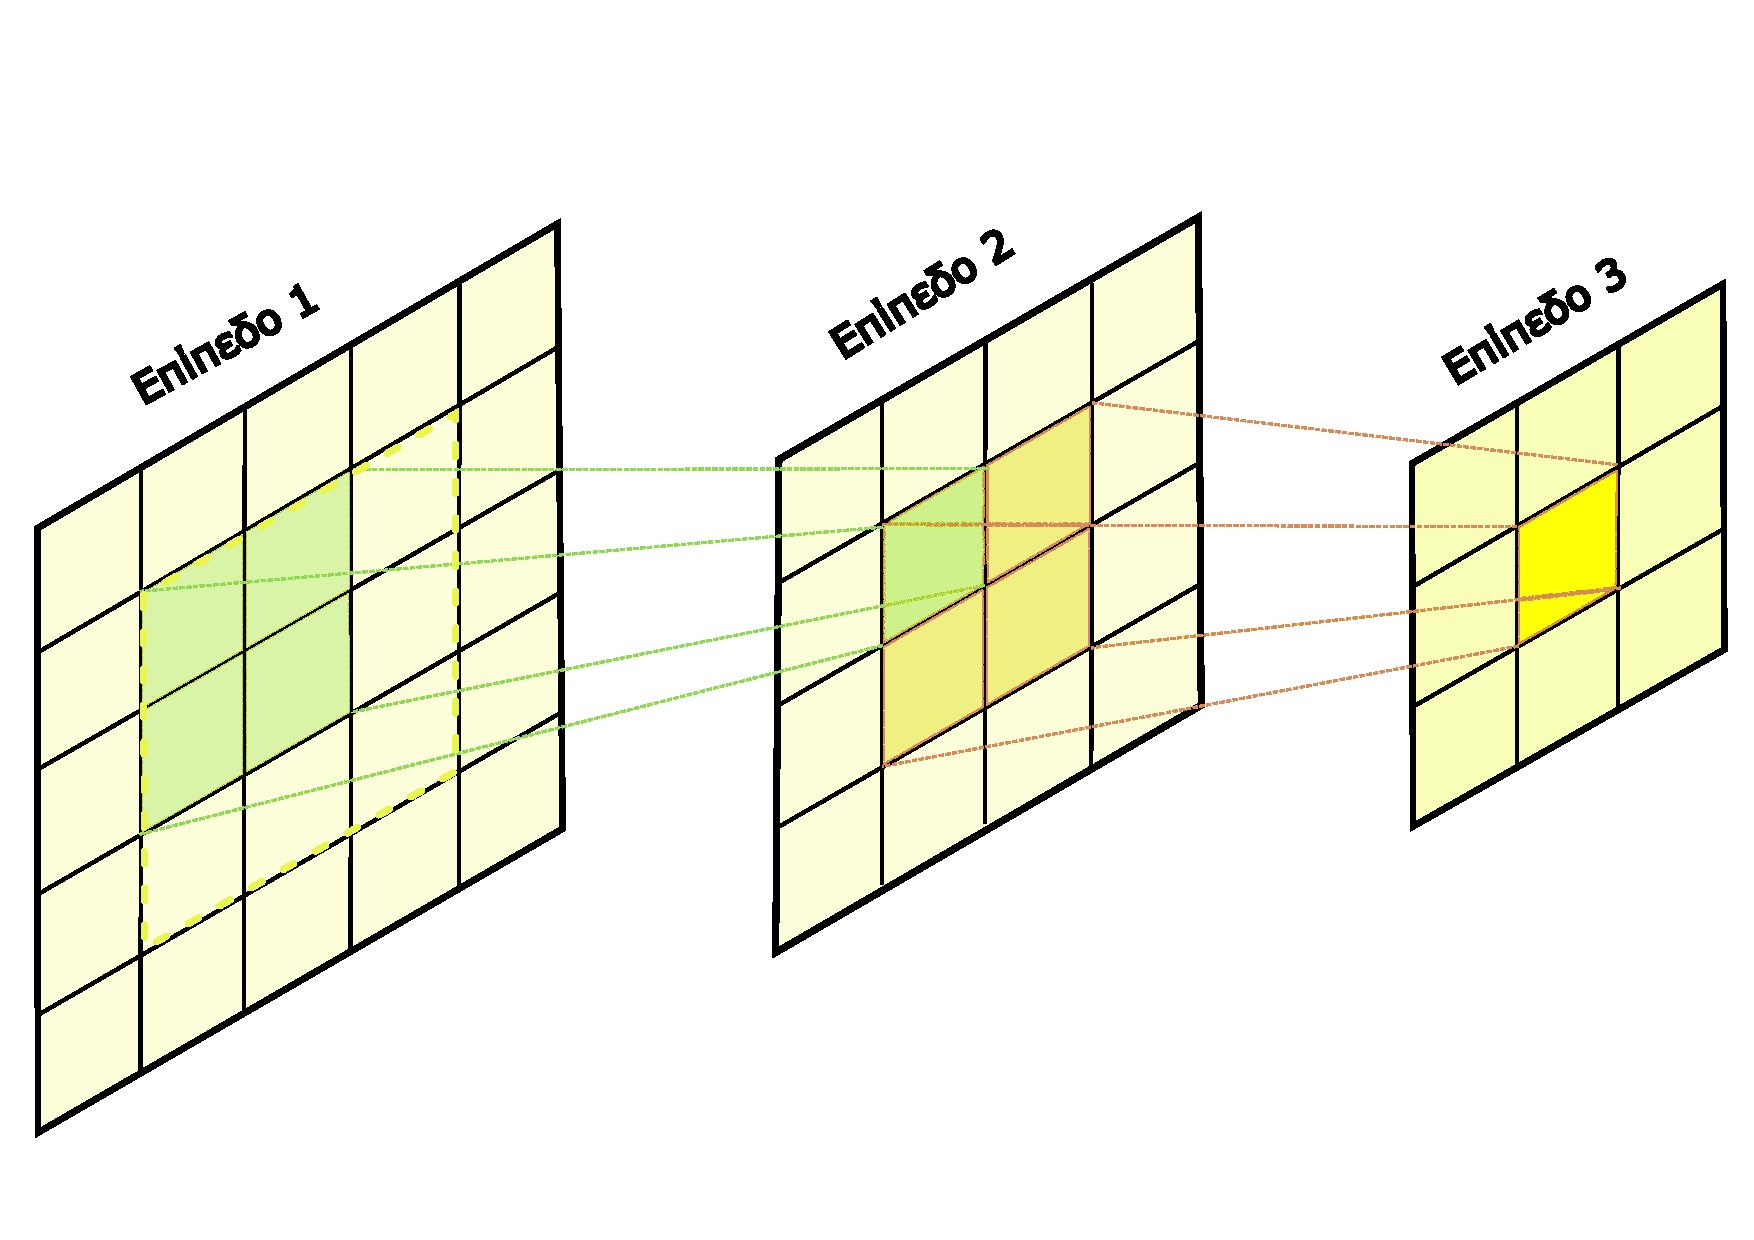
\includegraphics[width=0.7\textwidth]{images/chapter theoritical background/FOV_gr.pdf}
  \caption{Σχήμα τριών διαδοχικών συνελικτικών επιπέδων με μέγεθος φίλτρου $2\times2$ και βήμα 1. Όσο μεγαλύτερη είναι η απόσταση βάθους μεταξύ πρώτου και τελευταίου επιπέδου, τόσο μεγαλύτερο είναι το οπτικό πεδίο από το οποίο εξάγονται τα χαρακτηριστικά του τελικού επιπέδου. Στην εικόνα, το οπτικό πεδίο ενός στοιχείου στο τρίτο επίπεδο χάρτη χαρακτηριστικών σχηματίζει στο πρώτο επίπεδο ένα παραλληλόγραμμο $3\times3$ (απεικονίζεται με διακεκομμένες, κίτρινες γραμμές). \textit{Παράχθηκε από το \href{https://inkscape.org/}{\en{Inkscape}}.}} 
  \label{fig:fov}
\end{figure} 

\item Η ελαχιστοποίηση του υπολογιστικού κόστους (και των απαιτήσεων μνήμης) με την εφαρμογή των τοπικών φίλτρων (δηλαδή όχι πλήρως διασυνδεδεμένων) ως κυλιόμενων παραθύρων στον $x$ και $y$ άξονα πάνω στην εικόνα.
\end{itemize}
Από τα θετικά αυτά δομικά στοιχεία εμμέσως προκύπτει μια πολύ σημαντική ιδιότητα των συνελικτικών δικτύων: αυτή της μεταφοράς των διακυμάνσεων θέσης των αντικειμένων σε μια εικόνα εισόδου σε κατάλληλες εσωτερικές διακυμάνσεις των χαρτών χαρακτηριστικών (\en{translation equivariance}). Αναλυτικότερα, με τη μετακίνηση ενός αντικειμένου στην εικόνα κατά τον $x$ ή $y$ άξονα, λόγω της δισδιάστατης συνέλιξης, αυτή μεταφράζεται σε αντίστοιχη μετακίνηση των εξαχθέντων χαρακτηριστικών. Συνεπώς, θα μπορούσαμε να πούμε ότι ένα συνελικτικό νευρωνικό δίκτυο διαθέτει μηχανισμούς που να μοντελοποιούν τις οριζόντιες και κάθετες μετατοπίσεις της εισόδου ώστε αυτές να γίνονται αντιληπτές από το σύστημα.

\subsection{Βασικές Ανεπάρκειες των Συνελικτικών Νευρωνικών Δικτύων}
Το βασικό πρόβλημα που αντιμετωπίζουν οι αρχιτεκτονικές συνελικτικών νευρωνικών δικτύων που παρουσιάσαμε είναι η αδυναμία γενίκευσης σε νέες οπτικές γωνίες (\en{novel viewpoints}). Με άλλα λόγια, είναι σε θέση να αναγνωρίζουν αντικείμενα μόνο όταν βρίσκονται στον ίδιο προσανατολισμό, κλίμακα, διάτμηση (\en{orientation, scale, shear}) κ.τ.λ. με τα στιγμιότυπα αντικειμένων που απεικονίζονται στις εικόνες του συνόλου εκπαίδευσης. Έτσι λοιπόν, οι μόνοι αφινικοί μετασχηματισμοί (\en{affine transformations}) τους οποίους ένα συνελικτικό νευρωνικό δίκτυο μπορεί να χειριστεί αποδοτικά είναι οι μεταφορές (μεταθέσεις των αντικειμένων της εικόνας)\cite{sabour2017dynamic}.\par

Για την αναγνώριση αντικειμένων υπό νέες οπτικές γωνίες από τα συνελικτικά νευρωνικά δίκτυα χρησιμοποιούνται μη\textendashαποδοτικές μέθοδοι. Για παράδειγμα, μια μέθοδος είναι ο πολλαπλασιασμός των δεδομένων εισόδου μετά από τυχαία εφαρμογή μετασχηματισμών γνωστή ως \textquote{επαύξηση δεδομένων} (\en{data augmentation}). Μια άλλη μέθοδος που μπορεί να χρησιμοποιηθεί παράλληλα με την προηγούμενη είναι αυτή της ενσωμάτωσης επιπέδων μέγιστης συνάθροισης (\en{max pooling}). Όπως έχουμε αναφέρει, τα επίπεδα αυτά αυξάνουν την ευρωστία του συστήματος. Το επιτυγχάνουν, μέσω της υποδειγματοληψίας των χαρτών χαρακτηριστικών έτσι ώστε μικρές μεταβολές στη θέση (ή ακόμα και στον προσανατολισμό \cite{geron2019hands}) των αντικειμένων να μην αλλάζει τις αποκρίσεις (εξόδους) των φίλτρων των επακόλουθων επιπέδων. Η ιδιότητα αυτή ονομάζεται ανεξαρτησία υπό μεταφορά (\en{translation invariance}) και σε αντίθεση με την ιδιότητα των συνελικτικών επιπέδων που περιγράψαμε στην παράγραφο \ref{sec:positives_of_cnns}, οι μικρές διακυμάνσεις στην είσοδο του επιπέδου συνάθροισης απορρίπτονται και δε μοντελοποιούνται εσωτερικά του συστήματος. Με απλά λόγια, το σύστημα επιδιώκει να πετύχει γενίκευση στους αφινικούς μετασχηματισμούς κάτω από τους οποίους αναγνωρίζει τα αντικείμενα με το να αχρηστεύει την πληροφορία σχετικά με το συγκεκριμένο στιγμιότυπο εισόδου και να δημιουργεί μια ανεξάρτητη αναπαράσταση (εξαρτώμενη μόνο από το είδος του αντικειμένου) την οποία τα επόμενα επίπεδα θα επεξεργαστούν.\par

\begin{figure}[h]
  \centering
  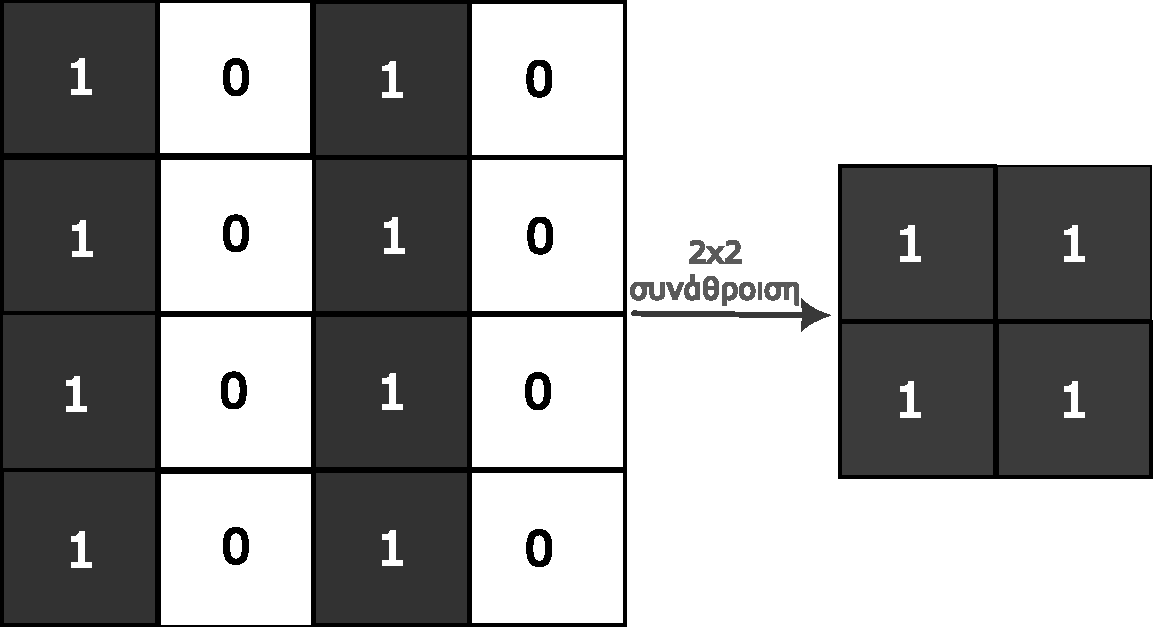
\includegraphics[width=0.7\textwidth]{images/chapter theoritical background/pool_invariance_1_gr.pdf}
  \caption{Σχήμα όπου εφαρμόζεται μέγιστη συνάθροιση με πυρήνα $2\times2$ και βήμα 2 σε μια δυαδική εικόνα δύο κάθετων ακμών. \textit{Παράχθηκε από το \href{https://inkscape.org/}{\en{Inkscape}}}.}
  \label{fig:poolinvar1}
\end{figure}

\begin{figure}[h]
  \centering
  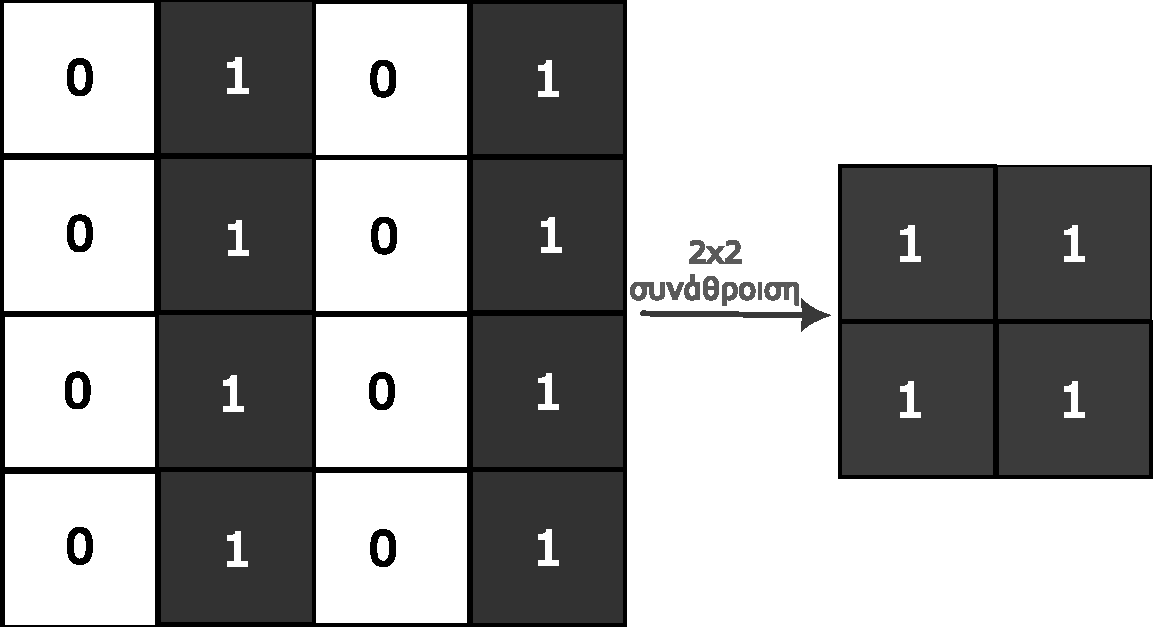
\includegraphics[width=0.7\textwidth]{images/chapter theoritical background/pool_invariance_2_gr.pdf}
  \caption{Σχήμα όπου εφαρμόζεται μέγιστη συνάθροιση με πυρήνα $2\times2$ και βήμα 2 σε μια δυαδική εικόνα δύο κάθετων ακμών, αφού η θέση λήψης μετατοπιστεί. Χάρη στο επίπεδο συνάθροισης, η απόκριση είναι ανεξάρτητη από μικρές μετατοπίσεις της εικόνας εισόδου. \textit{Παράχθηκε από το \href{https://inkscape.org/}{\en{Inkscape}}.}} 
  \label{fig:poolinvar2}
\end{figure} 

Σύμφωνα με τον \en{G. Hinton}\cite{youtubeHinton}, τα νευρωνικά δίκτυα θα πρέπει να χειρίζονται όλους τους αφινικούς μετασχηματισμούς με την ίδια λογική που διαχειρίζονται τα συνελικτικά επίπεδα τις κάθετες και οριζόντιες μετατοπίσεις. Δηλαδή, αντί να απορρίπτουν χρήσιμη πληροφορία μέσω των επιπέδων συνάθροισης να διαθέτουν μηχανισμούς που θα μοντελοποιούν εσωτερικά τις διακυμάνσεις στην οπτική γωνία των αντικείμενων. Η πρόταση αυτή βασίζεται στη σημαντική παρατήρηση ότι αλλαγές στη σκοπιά ενός αντικειμένου μεταβάλλουν με σύνθετο, μη γραμμικό τρόπο τα εικονοστοιχεία της εικόνας ενώ τροποποιούν με απλό, γραμμικό τρόπο τη μήτρα πόζας (\en{pose matrix}) του αντικειμένου\footnote{Οι μήτρες πόζας είναι πίνακες που περιγράφουν τη θέση και τον προσανατολισμό ενός αντικειμένου, δύο χαρακτηριστικά τα οποία μεταβάλλονται γραμμικά με την αλλαγή της οπτικής γωνίας θέασης ενός αντικειμένου. Χρησιμοποιούνται κατά κόρον στον χώρο των γραφικών με υπολογιστή για την περιγραφή του τρόπου τοποθέτησης των αντικειμένων σε έναν εικονικό κόσμο.}. Συνεπώς, φαίνεται ασύμφορη η προσπάθεια των συνελικτικών δικτύων να δημιουργούν ανεξάρτητες (υπό την οπτική γωνία) αναπαραστάσεις αντικειμένων απευθείας από τον χώρο των εικονοστοιχείων, χωρίς δηλαδή να λαμβάνουν υπόψη τη γραμμική σχέση μεταξύ των διακυμάνσεων της οπτικής γωνίας και των παραμέτρων του στιγμιότυπου (\en{instantiation parameters}) του αντικειμένου\footnote{Με τον όρο \textquote{παράμετροι στιγμιοτύπου} θα αναφερόμαστε κυρίως στην μήτρα πόζας του στιγμιοτύπου. Παρόλα αυτά, παράμετροι στιγμιοτύπου είναι και άλλοι παράγοντες που δεν εξαρτόνται από την κλάση του αντικειμένου προς αναγνώριση όπως ο φωτισμός, το μέγεθος ή χρώμα του αντικειμένου κ.τ.λ. }. Αντίθετα, θα ήταν πιο αποδοτική η μοντελοποίηση αυτής της γραμμικής σχέσης με έναν μηχανισμό ο οποίος θα πραγματοποιούσε ανάστροφα γραφικά (\en{inverse graphics}): θα αντιστοίχιζε τον χώρο των εικονοστοιχείων της εικόνας εισόδου σε έναν ιεραρχικό χώρο από μήτρες πόζας για το κάθε απεικονιζόμενο αντικείμενο. Σε αυτήν τη νέα αναπαράσταση, οι αφινικοί μετασχηματισμοί θα άλλαζαν με προβλέψιμο τρόπο τις \textemdashαπεπλεγμένες από το είδος του αντικειμένου\textemdash παραμέτρους των επιμέρους στιγμιοτύπων οδηγώντας στην επιθυμητή γενίκευση σε νέες οπτικές γωνίες.\par

Επιπρόσθετα, ο παρόν τρόπος διαχείρισης αφινικών μετασχηματισμών από τα συνελικτικά νευρωνικά δίκτυα τα καθιστά επιρρεπή σε αντιπαραθετική επίθεση (\en{adversarial attacks}). Αυτή τους η αδυναμία, θα μπορούσε να καταπολεμηθεί με την ενσωμάτωση ενός μηχανισμού που θα μοντελοποιούσε τις σχέσεις μεταξύ των τμημάτων ενός αντικειμένου ούτως ώστε, για την αναγνώρισή του, να λαμβάνονταν υπόψη η γεωμετρία των επιμέρους μερών του. Με άλλα λόγια, αν υπήρχε \textquote{αποθηκευμένη} στο νευρωνικό δίκτυο η πληροφορία για τον τρόπο σύνδεσης των στοιχείων που απαρτίζουν ένα αντικείμενο τότε θα ήταν περισσότερο εύρωστο σε αυτού του είδους τις επιθέσεις. Στο παράδειγμα του σχήματος \ref{fig:picasso_face} το συνελικτικό νευρωνικό δίκτυο αφενός δε διαθέτει κάποιο μηχανισμό να αναγνωρίζει την ακριβή θέση του ματιού στην εικόνα (αφού αυτή η πληροφορία απορρίπτεται σε ένα βαθμό μέσω των επιπέδων συνάθροισης) και αφετέρου, ακόμα και αν ήταν διαθέσιμη αυτή η πληροφορία, θα έμενε αναξιοποίητη διότι δεν αποθηκεύεται η γνώση για το ποια θα πρέπει να είναι η θέση του ματιού σε σχέση με τα υπόλοιπα μέρη. \par

\begin{figure}[h]
  \centering
  
\includegraphics[width=0.3\textwidth]{images/chapter theoritical background/picasso_problem_on_face.pdf}
  \caption{Σχήμα όπου απεικονίζεται το λεγόμενο πρόβλημα του \en{Picasso} στο οποίο η εικόνα έχει όλα τα σωστά μέρη αλλά οι σχέσεις μεταξύ τους είναι λάθος. Ένα υποθετικό συνελικτικό νευρωνικό δίκτυο θα δυσκολεύονταν να αντιληφθεί ότι το σχήμα της εικόνας δεν είναι κανονικό πρόσωπο. (Το παράδειγμα είναι ενδεικτικό αφού δεν έχει αποδειχθεί ότι ένα συνελικτικό δίκτυο θα αναγνώριζε το συγκεκριμένο παράδειγμα ως πρόσωπο.) \textit{Παράχθηκε από το \href{https://inkscape.org/}{\en{Inkscape}} τροποποιώντας \href{https://freesvg.org/vector-clip-art-of-long-thin-mans-face}{αυτή την εικόνα}.}} 
  \label{fig:picasso_face}
\end{figure}

Ένα τελευταίο σημείο αδυναμίας των κλασσικών νευρωνικών δικτύων είναι το λεγόμενο πρόβλημα της αποκλειστικής διάζευξης (\en{XOR problem})\cite{rumelhart1985learning_internal_representations}. Αυτό, προκύπτει από την παρατήρηση ότι η συνάρτηση της αποκλειστικής διάζευξης δεν μπορεί να υλοποιηθεί από έναν μεμονωμένο τεχνητό νευρώνα. Σύμφωνα με την περιγραφή του τεχνητού νευρώνα του σχήματος \ref{fig:_neural_node}, στον πυρήνα του προβλήματος βρίσκεται το γεγονός ότι δεν υπάρχει δυνατότητα σύγκρισης των εισόδων μεταξύ τους. Αντ' αυτού, πραγματοποιείται σύγκριση μεταξύ ενός διανύσματος εισόδων με ένα διάνυσμα (αποθηκευμένων) βαρών. Αυτή η αδυναμία όμως οδηγεί σε μη\textendashαποδοτικές λύσεις του προβλήματος (με την προσθήκη κρυφών επιπέδων). Επακόλουθη, λοιπόν, είναι η διάθεση πειραματισμού με ένα νέο είδος τεχνητού νευρώνα που θα μπορεί να συγκρίνει τις εισόδους (ή τα διανύσματα εισόδων) επιλύοντας το πρόβλημα της αποκλειστικής διάζευξης και κυρίως επιτρέποντας τον εντοπισμό συνδιακυμάνσεων στα χαρακτηριστικά εισόδου.


\subsection{Αρχές Λειτουργείας Νευρωνικών Δικτύων με Κάψουλες}
Στην προσπάθεια αντιμετώπισης των ανωτέρω μειονεκτημάτων των συνελικτικών νευρωνικών δικτύων σε εργασίες αυτόματης αναγνώρισης αντικειμένων, αναπτύχθηκαν τα νευρωνικά δίκτυα με κάψουλες. Αυτά διαμορφώθηκαν:
\begin{itemize}
  \item αντλώντας στοιχεία από την επιστήμη της νευροφυσιολογίας
  \item διατηρώντας αρκετά θετικά σημεία των συνελικτικών νευρωνικών δικτύων (π.χ. συνέλιξη)
  \item εισάγοντας τις ιεραρχικές δομές νευρώνων (κάψουλες) και έναν μηχανισμό για τη διασύνδεσή τους.
\end{itemize}

\subsubsection{Ορισμός Κάψουλας και Αρχές Λειτουργίας της}
Η κάψουλα δεν είναι τίποτα άλλο παρά μια ομάδα από νευρώνες. Κάθε κάψουλα έχει μια και μοναδική λειτουργία μέσα σε ένα νευρωνικό δίκτυο. Πιο συγκεκριμένα, κάθε μια εκπαιδεύεται να αναπαριστά την πιθανότητα παρουσίας και τις παραμέτρους στιγμιοτύπου μιας συγκεκριμένης οντότητας στο πεδίο υποδοχής της. Για παράδειγμα, σε μια εφαρμογή οπτικής αναγνώρισης του τύπου τροχοφόρων οχημάτων, μια κάψουλα θα μπορούσε να είναι επιφορτισμένη με την αναπαράσταση της οντότητας \textquote{ρόδα}. Σε περίπτωση που η οντότητα ήταν παρούσα στο πεδίο υποδοχής της αντίστοιχης κάψουλας τότε θα είχε ως έξοδο μεγάλη τιμή πιθανότητας παρουσίας και φυσικά τις τιμές που θα προσδιόριζαν τη θέση, τον προσανατολισμό, το μέγεθος κ.τ.λ. της αναγνωρισμένης ρόδας. Στο σημείο αυτό γίνεται αντιληπτό το πλεονέκτημα της χρήσης συστάδων από νευρώνες έναντι μεμονωμένων νευρώνων (όπως αυτός του σχήματος \ref{fig:_neural_node} που παράγει μια μονοδιάστατη τιμή εξόδου ή ενεργοποίησης) αφού έτσι γίνεται εφικτή η έξοδος πιο εκφραστικών, πολυδιάστατων αναπαραστάσεων.\par

Όπως είναι φυσικό, για την παραγωγή των παραμέτρων στιγμιοτύπου μιας οντότητας είναι απαραίτητη η διατήρηση ενός συστήματος αναφοράς για τη συγκεκριμένη οντότητα\footnote{Η αναγκαιότητα ύπαρξης συστήματος αναφοράς της οντότητας γίνεται ακόμα πιο προφανής αν αναλογιστεί κανείς ότι οι παράμετροι στιγμιοτύπου ουσιαστικά περιγράφουν τη σχέση μεταξύ μιας οντότητας υπό την οπτική γωνία λήψης της εικόνας και της αντίστοιχης οντότητας αναφοράς.} (βλ. σχήμα \ref{fig:ref_frame}). Αυτό είναι σύμφωνο με τις παρατηρήσεις λειτουργίας του ανθρώπινου οπτικού φλοιού που, όπως διατυπώσαμε, εφαρμόζει συστήματα αναφοράς σε κάθε οπτικό ερέθισμα. Το είδος και η γεωμετρία της οντότητας αναφοράς σχηματίζεται κατά τη διαδικασία εκμάθησης του νευρωνικού δικτύου. \par

\begin{figure}[h]
  \centering
  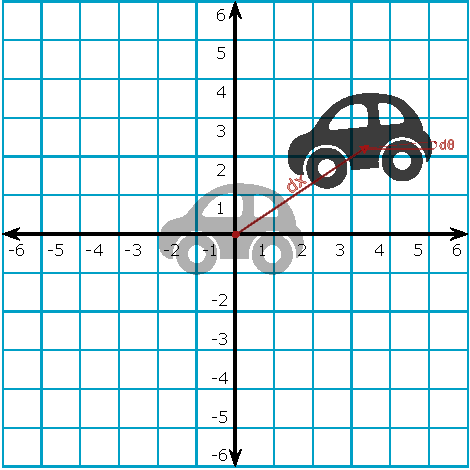
\includegraphics[width=0.5\textwidth]{images/chapter theoritical background/2D_Cartesian_Coordinates.pdf}
  \caption{Σχήμα όπου με τη βοήθεια μιας οντότητας αναφοράς (απεικονίζεται ως αχνό αυτοκίνητο) και του καρτεσιανού συστήματος συντεταγμένων υπολογίζονται οι παράμετροι στιγμιοτύπου (απόσταση από αρχή αξόνων και γωνία περιστροφής). \textit{Παράχθηκε από το \href{https://inkscape.org/}{\en{Inkscape}}}.}
  \label{fig:ref_frame}
\end{figure}

Με μαθηματικούς όρους, κάθε κάψουλα $c_i$ αποτελείται από ένα διάνυσμα $m_i \in \Re^d$ ή πίνακα $M_i \in \Re^{\surd{d}\times\surd{d}}$ από παραμέτρους στιγμιοτύπου και μια τιμή πιθανότητας παρουσίας $a_i \in [0,1]$. Η εξασφάλιση ότι η τιμή πιθανότητας ανήκει στο διάστημα $[0,1]$ γίνεται με την εφαρμογή μιας μη γραμμικής συνάρτησης ενεργοποίησης με σύνολο εξόδου το διάστημα αυτό. Σε ορισμένες υλοποιήσεις, η τιμή πιθανότητας παρουσίας της οντότητας που αναπαριστά η κάψουλα $c_i$ κωδικοποιείται στο μήκος του διανύσματος $m_i$.\par

\subsubsection{Οργάνωση των Καψουλών στο Νευρωνικό Δίκτυο}

Τα νευρωνικά δίκτυα από κάψουλες αξιοποιούν την τοπική χωρική συνεκτικότητα των εικόνων αφού οι κάψουλες οργανώνονται σε τρισδιάστατες δομές. Επίσης, αξιοποιούν την ιεραρχική δομή των φυσικών αντικειμένων με το να διατηρούν την πολυεπίπεδη διάταξη που χαρακτηρίζει τα συνελικτικά νευρωνικά δίκτυα (βλ. σχήμα \ref{fig:convolutional_caps_superimage}). Η διαφορά έγκειται στο γεγονός ότι αντί για επίπεδα από χάρτες χαρακτηριστικών υπάρχουν επίπεδα από κάψουλες (συμβολίζονται ως $C^{[l]}$)\footnote{Ιδιαίτερη προσοχή απαιτείται καθώς οι κάψουλες, αποτελούμενες από ένα σύνολο χαρακτηριστικών της οντότητας που αναγνωρίζουν, μπορούν να αντιπαραβληθούν με τους χάρτες χαρακτηριστικών (δηλαδή τον πίνακα τιμών ενεργοποίησης $A$). Θα ήταν λάθος λοιπόν να αντιπαραβληθούν με νευρώνες που έχουν αποθηκευμένα βάρη (βλ. σχήμα \ref{fig:conv_vs_caps_superimage}).}. Τα επίπεδα αυτά μπορεί να είναι πλήρως διασυνδεδεμένα ή να είναι συνελικτικά. Για παράδειγμα, στην περίπτωση των συνελικτικών επιπέδων από κάψουλες, αντί για παραγωγή χαρτών χαρακτηριστικών με μοναδιαίο βάθος ο καθένας, θα λέγαμε ότι παράγονται πλούσιοι σε πληροφορία χάρτες από διανύσματα ή πίνακες (πολυδιάστατες αναπαραστάσεις των αναγνωριζόμενων μοτίβων\textendashχαρακτηριστικών) που αποτελούν και το επόμενο επίπεδο από κάψουλες. Η παραγωγή του επόμενου επιπέδου από κάψουλες με βάση το προηγούμενο δε γίνεται με τη χρήση επιπέδων από νευρώνες αλλά πραγματοποιείται μέσω ενός αλγορίθμου \textquote{δρομολόγησης μέσω συμφωνίας} ο οποίος θα αναλυθεί στη συνέχεια.\par

\begin{figure}[h]
  \centering
  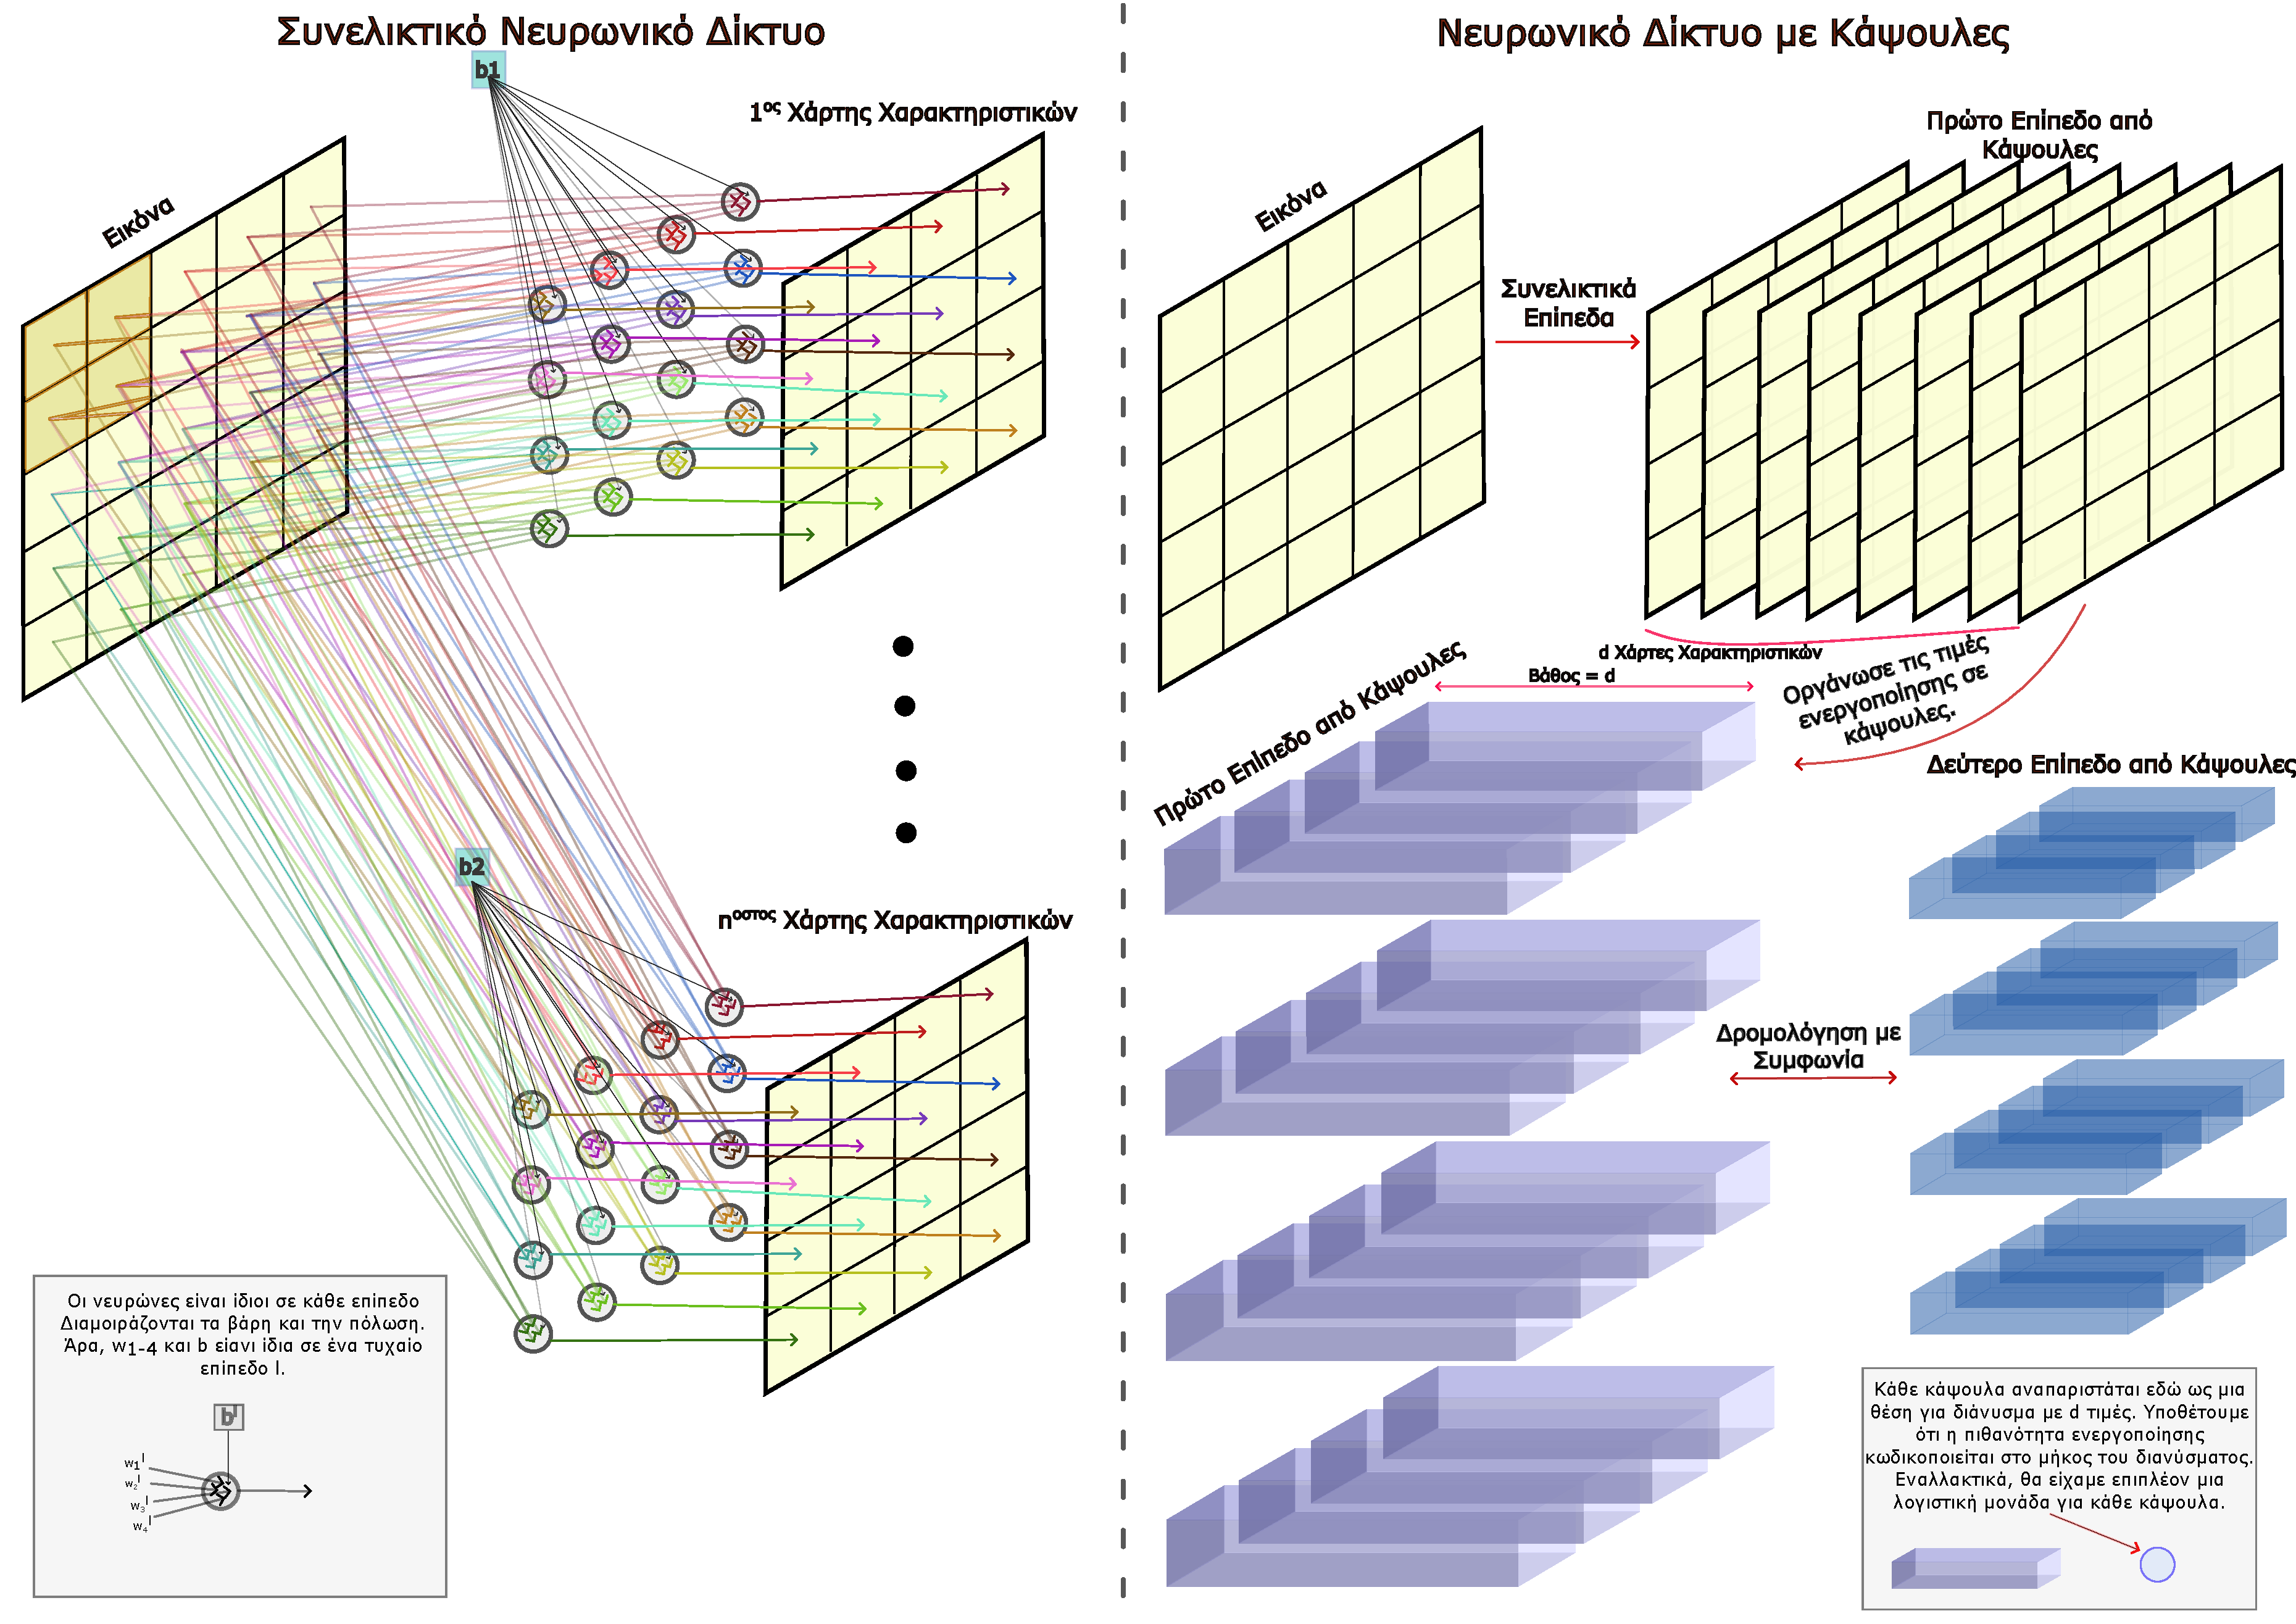
\includegraphics[width=0.95\textwidth]{images/chapter theoritical background/convolve_vs_capsule_gr.pdf}
  \caption{Δομικές διαφορές μεταξύ συνελικτικών νευρωνικών δικτύων και δικτύων με κάψουλες. Παρατηρούμε ότι οι κάψουλες δεν έχουν ομοιότητες με τους κλασικούς τεχνητούς νευρώνες. Κυρίως μπορούν να συσχετιστούν με σύνολα από χάρτες χαρακτηριστικών. \textit{Παράχθηκε από το \href{https://inkscape.org/}{\en{Inkscape}}}.}
  \label{fig:conv_vs_caps_superimage}
\end{figure}

\begin{figure}[h]
  \centering
  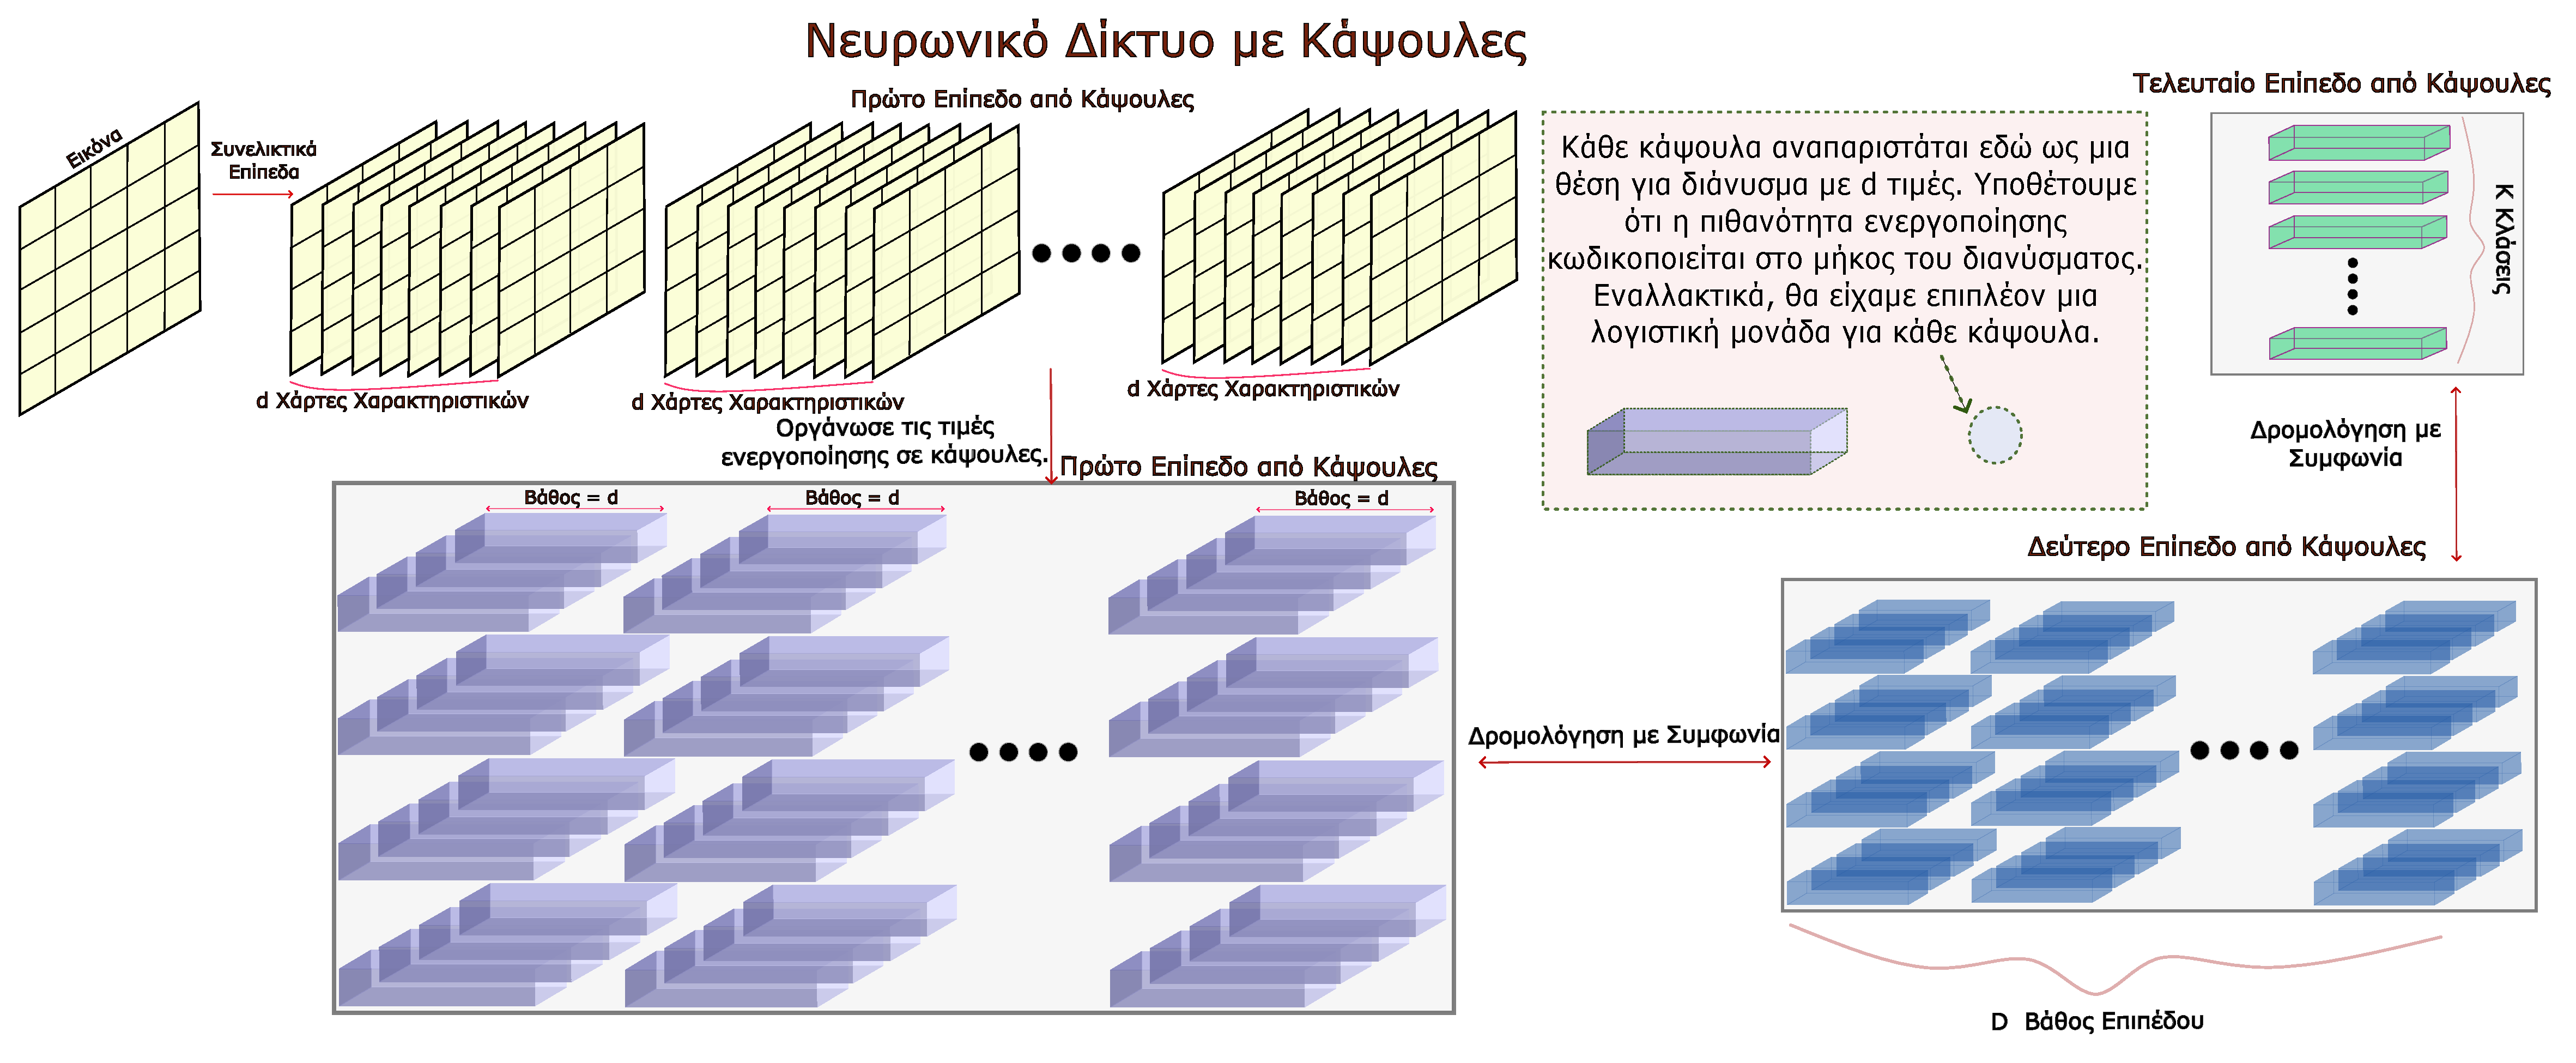
\includegraphics[width=0.95\textwidth]{images/chapter theoritical background/full_convolutional_capsule_layers_gr.pdf}
  \caption{Σχήμα όπου φαίνεται μια τυπική οργάνωση ενός νευρωνικού δικτύου με κάψουλες. \textit{Παράχθηκε από το \href{https://inkscape.org/}{\en{Inkscape}}}.}
  \label{fig:convolutional_caps_superimage}
\end{figure}

\subsubsection{Αλγόριθμος Δρομολόγησης με Συμφωνία}

Θα θέλαμε να εστιάσουμε στους υπολογισμούς που λαμβάνουν χώρα μεταξύ δύο διαδοχικών επιπέδων από κάψουλες. Αν και κάθε υλοποίηση είναι διαφορετική, θα παρουσιάσουμε υπό μια αφαιρετική σκοπιά τις βασικές αρχές που διέπουν τον κάθε αλγόριθμο δρομολόγησης. Επειδή σε ένα νευρωνικό δίκτυο από κάψουλες τα πρώτα επίπεδά του επιτελούν ιδιαίτερες λειτουργίες, ας υποθέσουμε χωρίς βλάβη της γενικότητας ότι το έχουμε τροφοδοτήσει με μια εικόνα και διαδοχικά έχουν υπολογιστεί ήδη οι τιμές των επιπέδων του μέχρι και το $l-1$. Θα επιθυμούσαμε στο σημείο αυτό να υπολογίσουμε τις τιμές για το επίπεδο $l$. \par

Με τους μέχρι τώρα υπολογισμούς, έχουμε στη διάθεσή μας μια τρισδιάστατη δομή από κάψουλες όπως φαίνεται στο σχήμα \ref{fig:convolutional_caps_superimage} σε μώβ χρώμα. Κάθε κάψουλα εμπεριέχει ένα σύνολο από τιμές που περιγράφουν την πόζα του τμήματος του αντικειμένου με το οποίο έχουν ταυτιστεί και αναγνωρίζουν. Επίσης, διαθέτουν και μια τιμή ενεργοποίησης που περιγράφει την πιθανότητα αυτό το τμήμα να είναι παρόν στο οπτικό πεδίο της κάψουλας. Κάψουλες με χαμηλή τιμή ενεργοποίησης θα λέμε ότι είναι ανενεργές και δε θα έχουν μεγάλη βαρύτητα στον υπολογισμό των τιμών του επόμενου επιπέδου. \par

Όπως είναι γνωστό, στο επίπεδο $l$ οι κάψουλες αναπαριστούν ανώτερες ιεραρχικά οντότητες σε σχέση με αυτές του επιπέδου $l-1$. Συνεπώς, η διαμόρφωση των τιμών του επιπέδου $l$ ανάγεται στο πρόβλημα της αντιστοίχησης (δρομολόγησης) επιμέρους τμημάτων των αντικειμένων σε μια εικόνα (αναπαριστώνται με κάψουλες $C{[l-1]}$) στα γενικότερα αντικείμενα που τα περιέχουν (αναπαριστώνται με τις κάψουλες $C^{[l]}$). Αυτή η δρομολόγηση προϋποθέτει την ύπαρξη ενός μηχανισμού που θα προβλέπει τις παραμέτρους που περιγράφουν τις γενικότερες οντότητες που αναγνωρίζουν οι κάψουλες $C^{[l]}$ με βάση τις παραμέτρους στιγμιοτύπων των επιμέρους οντοτήτων που αναγνωρίζουν οι κάψουλες $C^{[l-1]}$\footnote{π.χ. με βάση τη γεωμετρία της επιμέρους οντότητας \textquote{χέρι} να προβλέπεται η γεωμετρία της οντότητας \textquote{άνδρας}.}. O μηχανισμός υλοποιείται με πίνακες από βάρη $\boldsymbol{W}^{[l]}$ που αναλαμβάνουν να αποθηκεύσουν τις σχέσεις μέρους\textendash όλου (\en{part\textendash whole relationships}), δηλαδή τις σχέσεις όλων των δυνατών ζευγών μεταξύ των καψουλών επιπέδου $l-1$ και $l$. Έτσι αν στο επίπεδο $l-1$ έχουμε $n^{[l-1]}$ κάψουλες και στο επίπεδο $l$, $n^{[l]}$ τότε θα υπάρχουν $n^{[l-1]} \times n^{[l]}$ πίνακες βαρών μεταξύ των δύο επιπέδων. Μαθηματικά, η πρόβλεψη (ή ψήφο) για μια κάψουλα $c_j^{[l]}$ με βάση την κάψουλα $c_i^{[l-1]}$ παράγεται πολλαπλασιάζοντας τον πίνακα βαρών $W^{[l]}_{ij}$ με το διάνυσμα ή πίνακα παραμέτρων στιγμιότυπου $M_i^{[l-1]}$, δηλαδή $V^{[l]}_{ij} = M_i^{[l-1]}\times W^{[l]}_{ij}$. Να σημειώσουμε ότι τα βάρη $\boldsymbol{W}$ μαθαίνονται κατά την εκπαίδευση με τον αλγόριθμο της οπισθοδιάδοσης. \par

\begin{figure}[h]
  \centering
  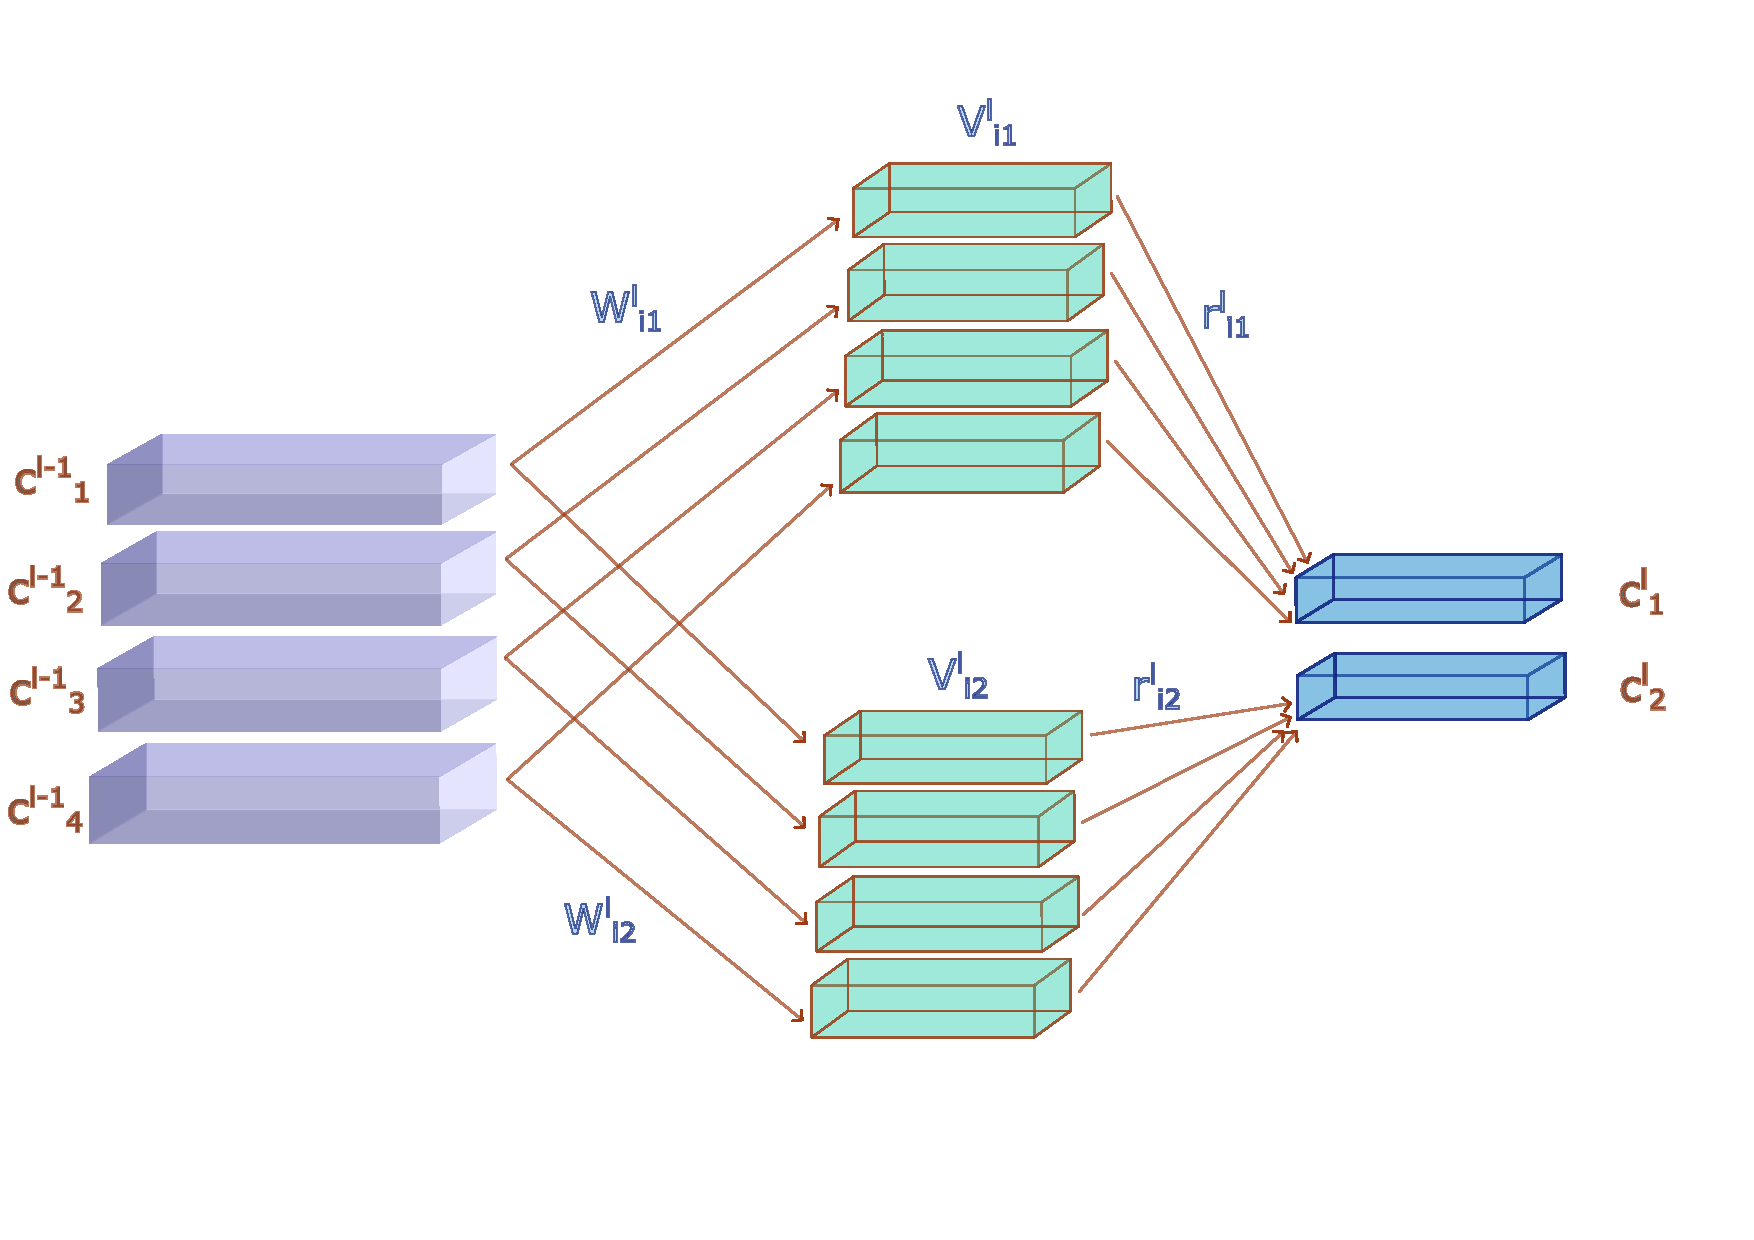
\includegraphics[width=0.95\textwidth]{images/chapter theoritical background/capsule_voting.pdf}
  \caption{Τρόπος παραγωγής των ψήφων για την απλή περίπτωση όπου έχουμε τέσσερεις κάψουλες στο επίπεδο $l-1$ και δύο στο επίπεδο $l$. Στο σχήμα, $i \in [1,4]$. Επίσης, η τιμή ενεργοποίησης θεωρήθηκε ότι κωδικοποιείται στο μήκος τω διανυσμάτων από παραμέτρους. \textit{Παράχθηκε από το \href{https://inkscape.org/}{\en{Inkscape}}}.}
  \label{fig:capsule_cast_votes}
\end{figure}

Μέχρι τώρα, έχουμε αναφέρει τον τρόπο με τον οποίο η κάθε μια κάψουλα $c^{[l]}$ διαθέτει $n^{[l-1]}$ προβλέψεις (μια από κάθε κάψουλα $c^{[l-1]}$) για το ποιες εκτιμά ότι είναι οι παράμετροι στιγμιοτύπου της $M^{[l]}$. Δεν έχουμε περιγράψει όμως τον τρόπο με τον οποίο αυτές οι προβλέψεις συγκροτούνται για την τελική διαμόρφωση των $\boldsymbol{M}^{[l]}$ και $\boldsymbol{a}^{[l]}$. Αυτό μας οδηγεί στην έννοια του φιλτραρίσματος μέσω της πολυδιάστατης σύμπτωσης (\en{high dimensional coincidence filtering}). Σύμφωνα με την έννοια αυτή, όταν μερικές από τις ψήφους των $C^{[l-1]}$ συμπέσουν σε μια γειτονιά του πολυδιάστατου χώρου των αναπαραστάσεων $\Re^{d}$ τότε αυτή η σύμπτωση δεν μπορεί να είναι τυχαία. Αντιθέτως, το γεγονός ότι μεγάλος αριθμός από κάψουλες $C^{[l-1]}$ συμφωνούν στο ποιες θα είναι οι τιμές παραμέτρων της εκάστοτε $c^{[l]}$ σημαίνει ότι πιθανότατα, αυτές είναι οι κατάλληλες τιμές της (και φυσικά ότι η οντότητα που εκπροσωπεί υπάρχει στην εικόνα). Έτσι η διαδικασία δρομολόγησης τελικά ανάγεται σε πρόβλημα εύρεσης συστάδων από ψήφους (\en{clusters of votes}) στον χώρο $\Re^{d}$.\par

Με βάση τα ανωτέρω, θα ήταν δυνατή η δρομολόγηση ενός τμήματος μιας οντότητας που αναπαριστάται από μια κάψουλα $c^{[l-1]}$ σε όλες τις κάψουλες $C^{[l]}$. Διαισθητικά, κάτι τέτοιο δεν είναι ορθό αφού ένα τμήμα ενός αντικειμένου δεν είναι δυνατό να αποτελεί μέρος όλων των αντικειμένων που αναπαριστώνται από τις κάψουλες του επόμενου επιπέδου. Επιπλέον, θα δημιουργούσε σύγχυση στον χώρο αναπαραστάσεων κατακλύζοντάς τον με περιττή πληροφορία. Συνεπώς, εισάγουμε τον περιορισμό ότι κάθε κάψουλα μπορεί να δρομολογεί τελικά την ψήφο της μόνο σε μια κάψουλα του επόμενου επιπέδου (\en{single parent assumption}). Με αυτόν τον τρόπο προκαλούμε ανταγωνισμό μεταξύ των $C^{[l]}$ να \textquote{εξηγήσουν} όσο το δυνατόν περισσότερες ψήφους των $C^{[l-1]}$\footnote{Χρησιμοποιούμε τον όρο \textquote{εξηγήσουν} διότι το σύνολο παραμέτρων $M^{[l]}$ που δημιουργείται για μια κάψουλα $c^{[l]}$ κατά μια έννοια εκφράζει τις απόψεις των $C^{[l-1]}$ που την ψήφισαν αναφορικά με το ποιο είναι το στιγμιότυπο του αντικειμένου που αναπαριστά.}.\par

Η κάθε κάψουλα $c^{[l-1]}$ είναι αδύνατο να γνωρίζει εκ των προτέρων (\en{a priori}) ποια κάψουλα του επόμενου επιπέδου (κάψουλα πατέρας) θα την εκφράζει καλύτερα αφού αυτό εξαρτάται όπως είπαμε από το αν η ψήφος της συμπέφτει μαζί με άλλες ψήφους στον χώρο αναπαραστάσεων (φιλτράρισμα πολυδιάστατης σύμπτωσης). Μονόδρομος λοιπόν είναι η επαναληπτική φύση του αλγορίθμου με συμφωνία κατά την οποία αρχικά οι ψήφοι της κάθε κάψουλας $c^{[l-1]}$, βεβαρημένες υπό μια ομοιόμορφη κατανομή διακριτής πιθανότητας, δρομολογούνται σε όλες τις $C^{[l]}$. Στη συνέχεια, μέσω του φιλτραρίσματος πολυδιάστατης σύμπτωσης, κάθε κάψουλα $c^{[l]}$ ανταγωνίζεται για να προσαρτήσει κάψουλες $c^{[l-1]}$ των οποίον οι ψήφοι σχηματίζουν συστάδες και άρα μπορεί εύκολα να \textquote{εξηγήσει}\footnote{Στον σχηματισμό συστάδων βοηθάει το γεγονός ότι οι κάψουλες του συνόλου $C^{[l]}$ βλέπουν διαφορετικές  ψήφους της κάθε κάψουλας του συνόλου $C^{[l-1]}$ αφού παράγονται μετά από πολλαπλασιασμό με διαφορετικό πίνακα βαρών. Έτσι, κάψουλες οι οποίες σχηματίζουν συστάδες από ψήφους στον χώρο αναπαράστασης μιας κάψουλας $c^{[l]}$ μπορεί στον χώρο αναπαράστασης μιας διαφορετικής κάψουλας να σχηματίζουν απόμακρες προβλέψεις.}. Χωρίς βλάβη της γενικότητας, κάθε κάψουλα $c^{[l]}$ \textquote{εξηγεί} τις ψήφους προσαρμόζοντας τον πίνακα (ή το διάνυσμα) $M^{[l]}$ στο κέντρο βάρους των ψήφων. Επιπρόσθετα, προσαρμόζει την τιμή πιθανότητας ενεργοποίησής της ανάλογα με το πόσο καλά εξηγεί τις ψήφους\footnote{Ο μηχανισμός υπολογισμού πιθανότητας ενεργοποίησης $a^{[l]}$ διαφέρει σημαντικά από υλοποίηση σε υλοποίηση αλλά γενικά είναι ανάλογο του αριθμού από κάψουλες $C^{[l-1]}$ που προτιμούν την κάψουλα $c^{[l]}$ και της πυκνότητας των ψήφων τους.}. Αυτές οι δύο προσαρμογές ανατροφοδοτούνται πίσω στις κάψουλες $c^{[l-1]}$ οι οποίες αλλάζουν, η κάθε μία, την κατανομή των βαρών υπό τα οποία δρομολογούν τις ψήφους τους (\en{coupling coefficients}) έτσι ώστε να προτιμούν κάψουλες γονείς που είναι ενεργές και εκφράζουν καλύτερα την ψήφο τους (το διάνυσμα της ψήφου τους είναι πιο κοντά στο διάνυσμα $M^{[l]}$). Όσο εξελίσσονται οι επαναλήψεις, τόσο οι κάψουλες $c^{[l-1]}$ είναι πιο σίγουρες για το που θα αποστείλουν τις ψήφους τους (η ομοιόμορφη κατανομή εκφυλίζεται σε ένα σημείο\textendash κάψουλα) και οι πίνακες $\boldsymbol{M}^{[l]}$ συγκλίνουν στο κέντρο των συστάδων από ψήφους.\par

Συγκεντρωτικά, μπορούμε να παρουσιάσουμε έναν αφαιρετικό αλγόριθμο δρομολόγησης με συμφωνία μεταξύ δύο διαδοχικών επιπέδων από κάψουλες $l-1$ και $l$ ως εξής:

\begin{enumerate}
  \item Για κάθε κάψουλα $c_i^{[l-1]} \in C^{[l-1]}$ υπολόγισε τις ψήφους\textendash προβλέψεις ως $V_{ij}=M_i \times W_{ij}$
  \item Αρχικοποίησε τις τιμές βαρών δρομολόγησης $r_{ij}=1/n^{[l]},\forall i \in [1,n^{[l-1]}],\forall j \in [1,n^{[l]}]$ έτσι ώστε $\sum_{j = 1}^{n^{[l]}}r_{ij} = 1$.
  \item Επανέλαβε για προκαθορισμένο αριθμό επαναλήψεων:
  \begin{enumerate}
    \item Για καθεμία κάψουλα $c_j^{[l]}$ εντόπισε τις συστάδες από βεβαρημένες ψήφους στον χώρο αναπαράστασης $\Re^d$ και με βάση αυτές υπολόγισε τις παραμέτρους στιγμιοτύπου $M_j^{[l]}$ που θα τις εκφράζει, $\forall j \in [1,n{[l]}]$.
    \item Υπολόγισε για καθεμία κάψουλα $c_j^{[l]}$ την τιμή ενεργοποίησής της με βάση το πόσο καλά εξηγεί τα δεδομένα.
    \item Για κάθε κάψουλα $c_i^{[l-1]}$ ενημέρωσε τα βάρη δρομολόγησης $r_{ij}, \forall j \in [1,n^{[l]}]$ ώστε να δίνεται μεγαλύτερο βάρος σε κάψουλες γονείς των οποίων οι παράμετροι στιγμιοτύπου εξηγούν καλύτερα τις ψήφους.
  \end{enumerate}
    
  \item Τερμάτισε με έξοδο $\boldsymbol{M}^{[l]}$ και $\boldsymbol{a}^{[l]}$.
\end{enumerate}

Ας φανταστούμε τώρα ότι έχουμε πολλά διαδοχικά επίπεδα από κάψουλες. Με τον αλγόριθμο δρομολόγησης (και λόγο της υπόθεσης μοναδικού πατέρα), δημιουργείται δυναμικά κατά την πρόσθια τροφοδότηση του δικτύου ένα ιεραρχικό δέντρο από ενεργές κάψουλες όπου η κάθε μια αναπαριστά τις οντότητες που βρίσκονται στην εικόνα. Ο σχηματισμός του ιεραρχικού δέντρου θα μπορούσε να παρομοιαστεί με το σκάλισμα ενός γλυπτού από ένα κομμάτι μαρμάρου \cite{sabour2017dynamic}. Το μάρμαρο είναι όλες οι κάψουλες σε κάθε επίπεδο ενώ η διαδικασία σκαλίσματος πραγματοποιείται από τον αλγόριθμο δρομολόγησης με συμφωνία που επιλεκτικά συνδέει και ενεργοποιεί ορισμένες κάψουλες. Επειδή η κάθε κάψουλα αναπαριστά όχι μόνο την πιθανότητα ύπαρξης της οντότητας αλλά και τις παραμέτρους στιγμιοτύπου της, μπορούμε να υποθέσουμε (χρησιμοποιώντας την ορολογία της προηγούμενης υποενότητας) ότι η ιεραρχική δομή είναι εμπλουτισμένη. Με άλλα λόγια, η δενδροειδής δομή από τις ενεργές κάψουλες που σχηματίζεται δυναμικά κατά την πορόσθια τροφοδότηση δε μοντελοποιεί μόνο την ιεραρχία μεταξύ ενός αντικειμένου και των μερών του (με σχέσεις τύπου κόμβοι γονέων $\supseteq$ κόμβοι παιδιών) αλλά και τις γεωμετρικές σχέσεις μεταξύ αυτών (π.χ. σε ποια θέση τοποθετούνται τα επιμέρους τμήματα για να συνθέσουν το όλον).\par


\subsubsection{Πρώτα Επίπεδα ενός Νευρωνικού Δικτύου με Κάψουλες}
Τα πρώτα επίπεδα ενός νευρωνικού δικτύου, όπως προκύπτει από τη μέχρι τώρα ανάλυση, είναι επιφορτισμένα με τον μετασχηματισμό από τον χώρο των εικονοστοιχείων στον χώρο αναπαράστασης των παραμέτρων στιγμιοτύπων\footnote{Υπενθυμίζουμε ότι στον χώρο αυτό, οι αλλαγές στην οπτική γωνία προκαλούν γραμμικές μεταβολές στις παραμέτρους (στα χαρακτηριστικά).} ώστε να μπορούν μετά σε αυτό να δράσουν οι κάψουλες. Πρακτικά, πρόκειται για συνελικτικά επίπεδα από κλασσικούς νευρώνες που παράγουν χάρτες χαρακτηριστικών που αποτελούνται από βαθμωτά μεγέθη. Στη συνέχεια αυτά τα βαθμωτά μεγέθη ομαδοποιούνται σε διανύσματα ή πίνακες ούτος ώστε κάθε ομάδα να ενθυλακώνει τις παραμέτρους μιας κάψουλας. Μέσω εκπαίδευσης, τα πρώτα επίπεδα μαθαίνουν να πραγματοποιούν ανάστροφα γραφικά (\en{derendering})\footnote{Ουσιασιαστικά πραγγματοποιούν μη παραμετρικό μετασχηματισμό \en{Hough}.} και να παράγουν αυτό που ονομάζουμε \textquote{αρχείο σκηνής} (βλ. παράρτημα \ref{chap:definitions}). Αυτή τη λειτουργία δε διαθέτουν τα κλασσικά συνελικτικά νευρωνικά δίκτυα διότι οφείλεται στους δομικούς και λειτουργικούς περιορισμούς που επιβάλει το νευρωνικό δίκτυο από κάψουλες.\par

\subsubsection{Τελευταίο Επίπεδο ενός Νευρωνικού Δικτύου με Κάψουλες}
Συνήθως, το τελευταίο επίπεδο ενός τέτοιου δικτύου είναι ένα επίπεδο από κάψουλες (όπως φαίνεται στο σχήμα \ref{fig:convolutional_caps_superimage}). Στις περισσότερες περιπτώσεις για εφαρμογές ταξινόμησης, υπάρχει μία κάψουλα ανά κατηγορία. Η πρόβλεψη $\hat{y}$ του νευρωνικού δικτύου λαμβάνεται ως η οντότητα που εκπροσωπείται από την κάψουλα του τελευταίου επιπέδου που έχει την μεγαλύτερη τιμή ενεργοποίησης (για την συγκεκριμένη είσοδο).

\subsubsection{Πως τα Νευρωνικά Δίκτυα με Κάψουλες Γενικεύουν σε Νέες Οπτικές Γωνίες}
Ο κύριος λόγος της αποδοτικής γενίκευσης των νευρωνικών δικτύων με κάψουλες αποδίδεται στο ότι εργάζονται στον χώρο παραμέτρων των στιγμιοτύπων μιας εικόνας (ονομάζεται και χώρος αναπαράστασης γραφικών) όπου οι αλλαγές στην οπτική γωνία προκαλούν γραμμικές μεταβολές στις παραμέτρους. Έχοντας διαχωρίσει τους παράγοντες διακύμανσης της κάθε οντότητας (την πιθανότητα ύπαρξής από τις παραμέτρους στιγμιοτύπου της), και έχοντας μεταβεί σε έναν χώρο όπου αλλαγές στην οπτική γωνία αλλάζουν με γραμμικό τρόπο τα χαρακτηριστικά στιγμιοτύπου, η γενίκευση σε νέες οπτικές γωνίες έγκειται απλά στη γραμμική παρεμβολή των χαρακτηριστικών αυτών. Έτσι, στο απλό παράδειγμα που το δίκτυο έχει εκπαιδευτεί να αναγνωρίζει ένα ψηφίο στραμμένο με τυχαίο τρόπο κατά $\theta^\circ \in [-5,+5]$ τότε θα διαθέτει κάποια κάψουλα $c_i^{[L]}$ που αναγνωρίζει την ύπαρξη αυτού του ψηφίου με πιθανότητα $a_i^{[L]}$ και κωδικοποιεί τον προσανατολισμό του (μεταξύ άλλων χαρακτηριστικών) στον πίνακα $M_i^{[L]}$. Έτσι, μπορεί εύκολα να προβλέψει μέσω παρεμβολής τι επίδραση θα έχει η στρέψη του ψηφίου κατά $+10^\circ$.\footnote{Η στρέψη του ψηφίου κατά +10 μοίρες είναι ισοδύναμε με τη στρέψη της κάμερας κατά -10 μοίρες. Συνεπώς, αποτελεί μια νέα οπτική γωνία για την οποία το δίκτυο δεν έχει εκπαιδευτεί.}\par

Για να επιτευχθεί γενίκευση σε νέες οπτικές γωνίες, όλες οι σχεδιαστικές αποφάσεις των νευρωνικών δικτύων με κάψουλες εξυπηρετούν έμμεσα ή άμεσα την εσωτερική μοντελοποίηση των αλλαγών στις διακυμάνσεις της. Για παράδειγμα, δε χρησιμοποιούνται επίπεδα συνάθροισης καθώς αυτά όπως έχουμε αναφέρει οδηγούν σε αναπαραστάσεις, ανεξάρτητες της οπτικής γωνίας. Επιπλέον, χρησιμοποιούν κάψουλες και όχι χάρτες από βαθμωτά χαρακτηριστικά καθώς μέσω των πρώτων μπορούν να αναπαριστούν σε ένα διάνυσμα πλούσια πληροφορία σχετικά με τη γεωμετρία του αντικειμένου που αναγνωρίζουν (η πληροφορία αυτή θα ήταν αδύνατο να κωδικοποιηθεί σε μια μεμονωμένη τιμή). Οι παράμετροι στιγμιοτύπου μιας κάψουλας που αφορούν το αντικείμενο που αναπαριστούν αλλάζουν με προβλέψιμο τρόπο καθώς το αντικείμενο μετακινείται στην πολλαπλότητα των δυνατών απεικονίσεων (\en{manifold of possible appearances}). Συνεπώς, οι αλλαγές στην οπτική γωνία μεταφέρονται με αποδοτικό τρόπο μέσα από το σύστημα. Αντίθετα, η τιμή πιθανότητας ύπαρξης του αντικειμένου που αναγνωρίζει η κάθε κάψουλα στο πεδίο υποδοχής της επιθυμούμε να είναι όσο το δυνατό ανεξάρτητη από τον τρόπο απεικόνισης του αντικειμένου\footnote{Στις μέχρι τώρα κύριες υλοποιήσεις, δεν υπάρχει πλήρης ανεξαρτησία σε όλο το φάσμα των πιθανών απεικονίσεων.}. Επίσης, ανεξάρτητοι επιβάλουμε να είναι οι πίνακες $\boldsymbol{W}$ που αποθηκεύουν τις σχέσεις μεταξύ μερών και του όλου\footnote{Προφανώς, όπως και στα γραφικά υπολογιστή, ο πίνακας μετασχηματισμού που εκφράζει τις σχέσεις μέρους\textendash όλου είναι ανεξάρτητος από την εκάστοτε οπτική γωνία του στιγμιοτύπου.}. Ένα τελευταίο παράδειγμα που συμβάλλει έμμεσα στην επίτευξη γενίκευσης σε μεταβολές οπτικής γωνίας είναι η ενσωμάτωση του αλγορίθμου δρομολόγησης με συμφωνία. Εκτός από τον ρόλο που περιγράψαμε στο να διαμορφώνει τις κάψουλες του επόμενου επιπέδου, είναι πολύ σημαντικό ότι εντοπίζει συνδιακυμάνσεις μεταξύ των αναπαραστάσεων εισόδου\footnote{Ισοδύναμα, δεν υποφέρει από το πρόβλημα της αποκλειστικής διάζευξης.} συγκρίνοντας τα διανύσματα ψήφων μεταξύ τους μέσω του φιλτραρίσματος πολυδιάστατης σύμπτωσης.

\subsubsection{Απλό Παράδειγμα Εφαρμογής Αλγορίθμου Δρομολόγησης με Συμφωνία}

\begin{figure}[p]
  \centering
  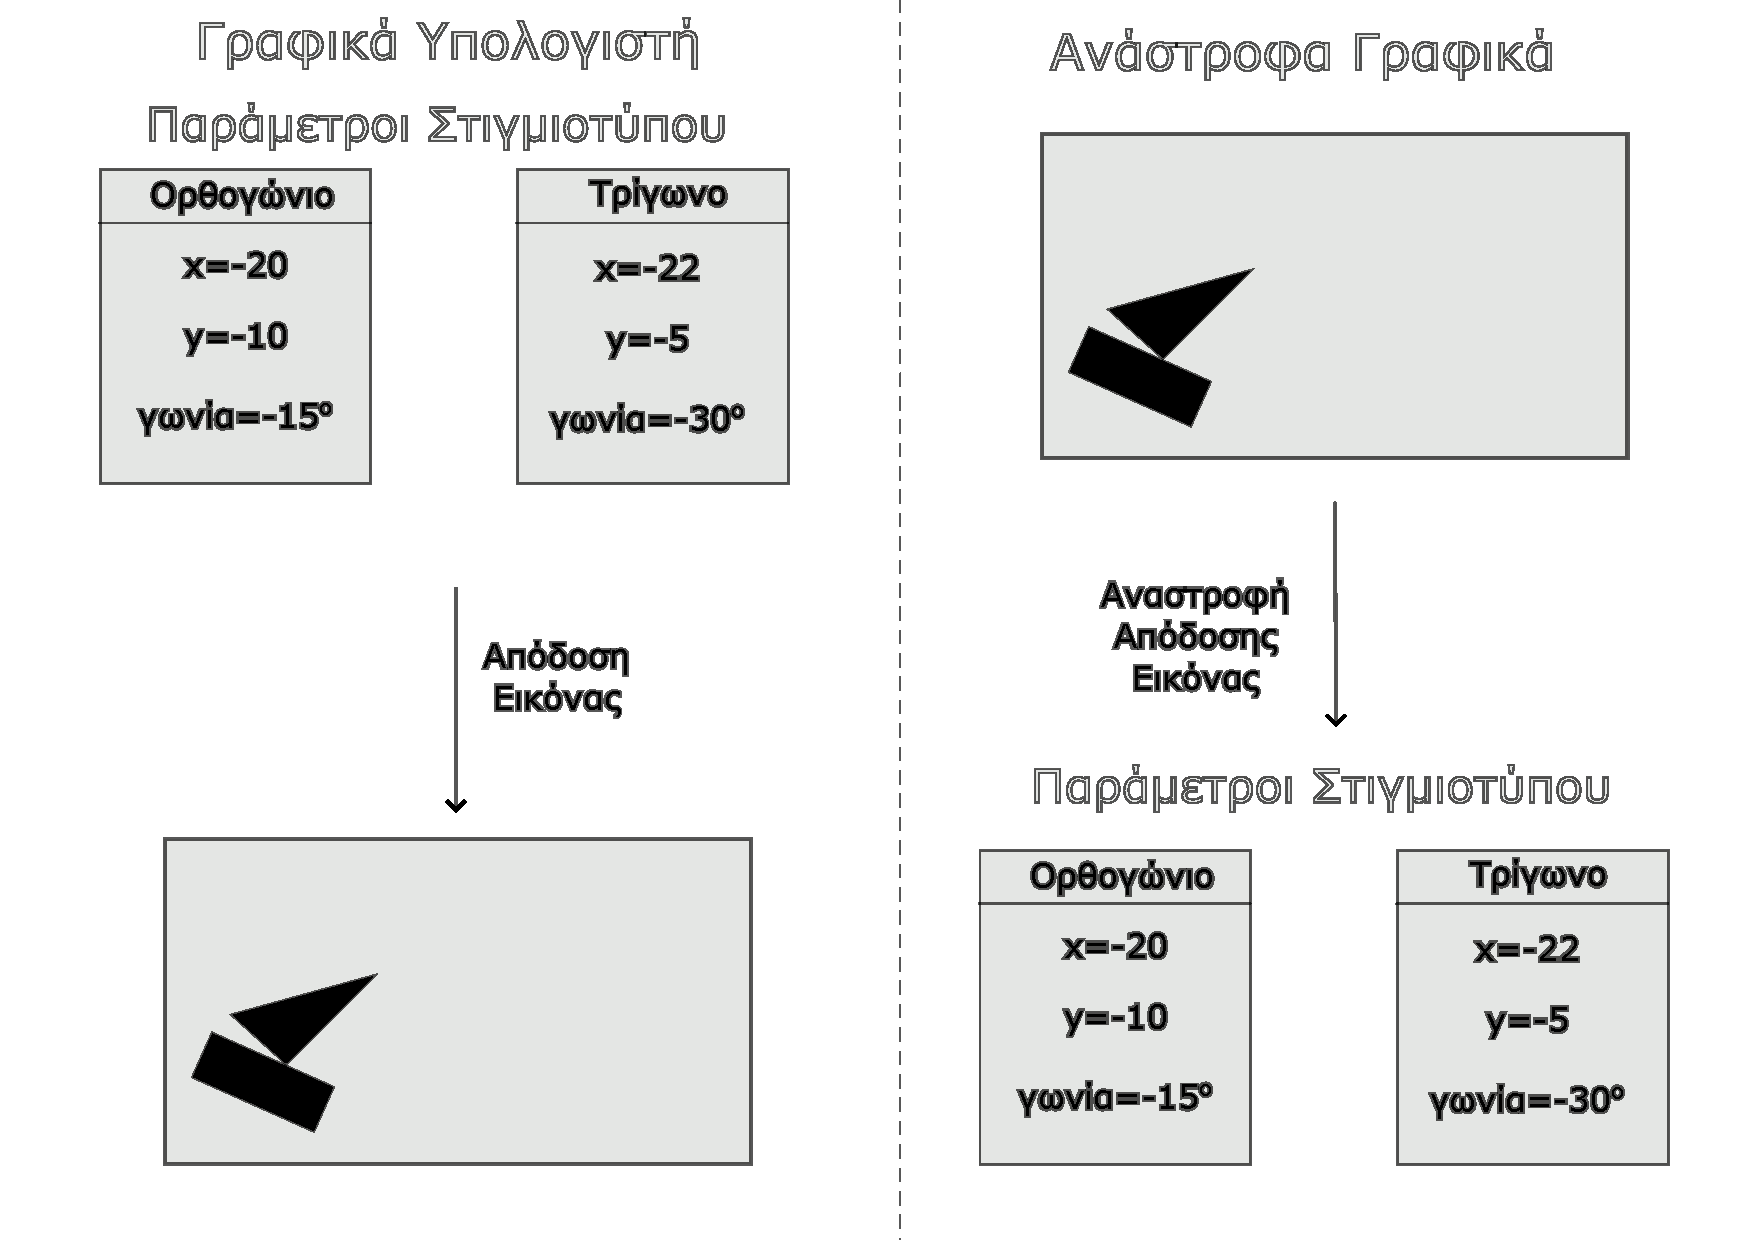
\includegraphics[width=0.8\textwidth]{images/chapter theoritical background/render_derender_gr.pdf}
  \caption{Η διαδικασία ανάστροφων γραφικών που επιχειρείται από τα νευρωνικά δίκτυα από κάψουλες. Στο σχήμα, αντιπαραβάλλεται με τη διεργασία της απόδοσης εικόνας (\en{rendering}). \textit{Παράχθηκε από το \href{https://inkscape.org/}{\en{Inkscape}}}.}
  \label{fig:render_derender}
\end{figure}

Στο απλό παράδειγμα που εξετάζουμε\cite{geron2019hands}, ας υποθέσουμε ότι κάθε κάψουλα έχει ως παραμέτρους στιγμιοτύπου τις τιμές που προσδιορίζουν τη θέση του αντικειμένου ($x,y$) και την τιμή $\theta$ του προσανατολισμού. Όπως αναφέραμε, στόχος είναι να γίνουν ανάστροφα γραφικά όπως φαίνεται και στο σχήμα \ref{fig:render_derender}. Η αναπαράσταση των τιμών μιας κάψουλας στο παράδειγμά μας θα γίνεται με ένα διάνυσμα του οποίου ο προσανατολισμός θα κωδικοποιεί τις παραμέτρους στιγμιοτύπου και το μήκος του την τιμή ενεργοποίησης. Όσο μεγαλύτερο το μήκος, τόσο πιο σίγουρη είναι η κάψουλα για την ύπαρξη της οντότητας που αναγνωρίζει. Ας υποθέσουμε ότι έχουμε δύο είδη από κάψουλες στο πρώτο επίπεδο (σχηματίζονται συνήθως από συνελικτικά επίπεδα)· αυτές που αναγνωρίζουν ορθογώνιο και αυτές που αναγνωρίζουν τρίγωνο (στο σχήμα \ref{fig:caps_vectors} συμβολίζονται με πράσινα και μπλε βέλη αντίστοιχα). Τα δύο είδη από κάψουλες διαμοιράζονται στον χώρο όπως τα φίλτρα στα συνελικτικά επίπεδα. Στο σχήμα \ref{fig:caps_vectors} παρατηρούμε ότι όλες οι κάψουλες έχουν μικρά διανύσματα εκτός από τις δύο που έχουν πεδίο υποδοχής το μέρος της εικόνας όπου τοποθετείται το τρίγωνο και το τετράγωνο. \par


\begin{figure}[p]
  \centering
  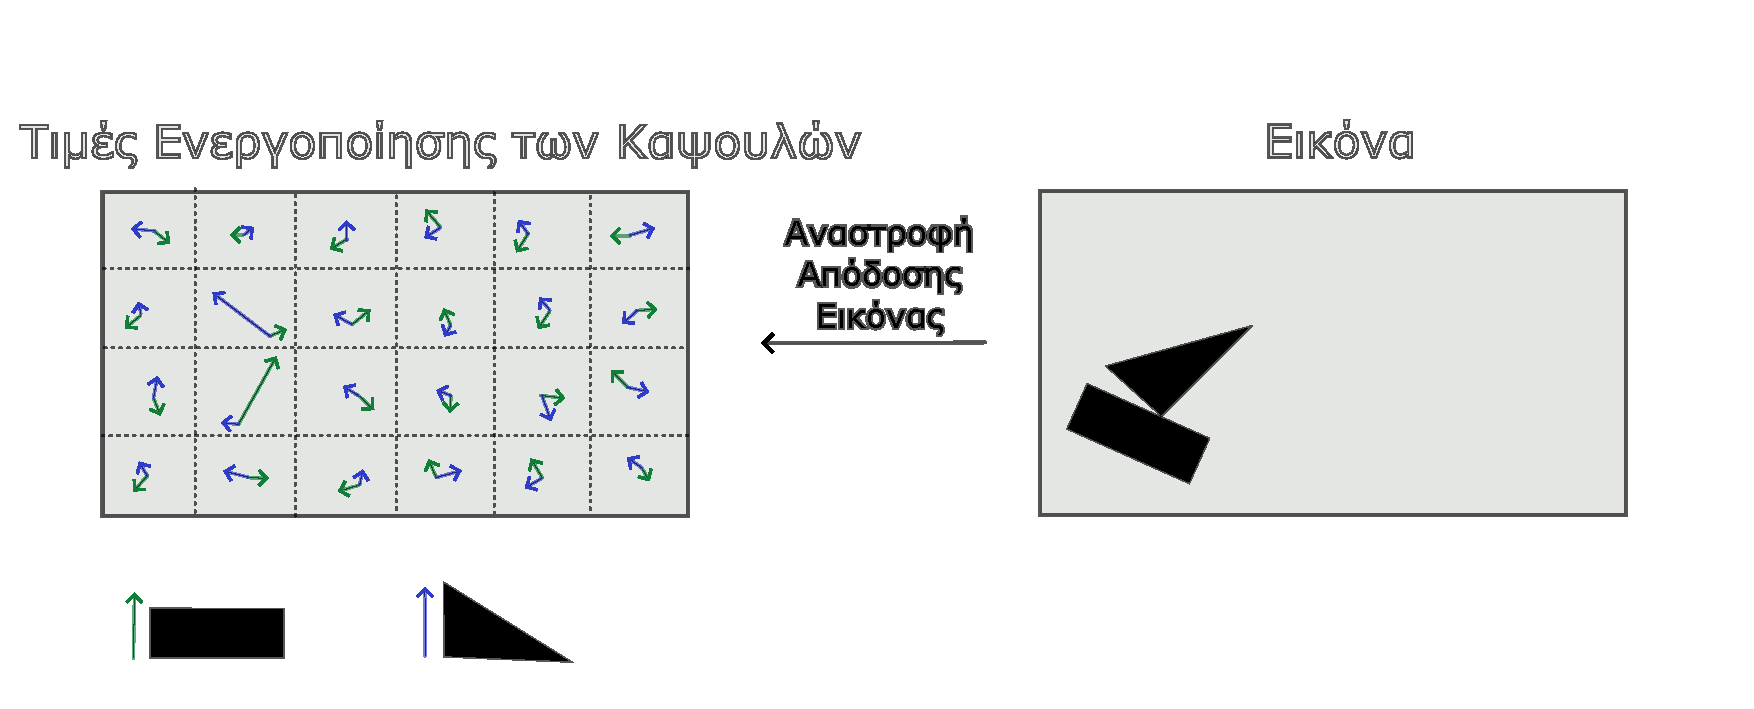
\includegraphics[width=0.8\textwidth]{images/chapter theoritical background/caps_vectors_gr.pdf}
  \caption{Τιμές ενεργοποίησης όπως προκύπτουν από ένα συνελικτικό επίπεδο καψουλών που αναγνωρίζουν δύο οντότητες: ορθογώνιο και τρίγωνο. Οι κάψουλες αυτού του επιπέδου θα μπορούσε να είναι το αποτέλεσμα συνελικτικών επιπέδων από νευρώνες (στην περίπτωση αρχικών επιπέδων) ή το αποτέλεσμα δρομολόγησης μέσω συμφωνίας από προηγούμενο επίπεδο καψουλών. \textit{Παράχθηκε από το \href{https://inkscape.org/}{\en{Inkscape}}}.}
  \label{fig:caps_vectors}
\end{figure}

\begin{figure}[p]
  \centering
  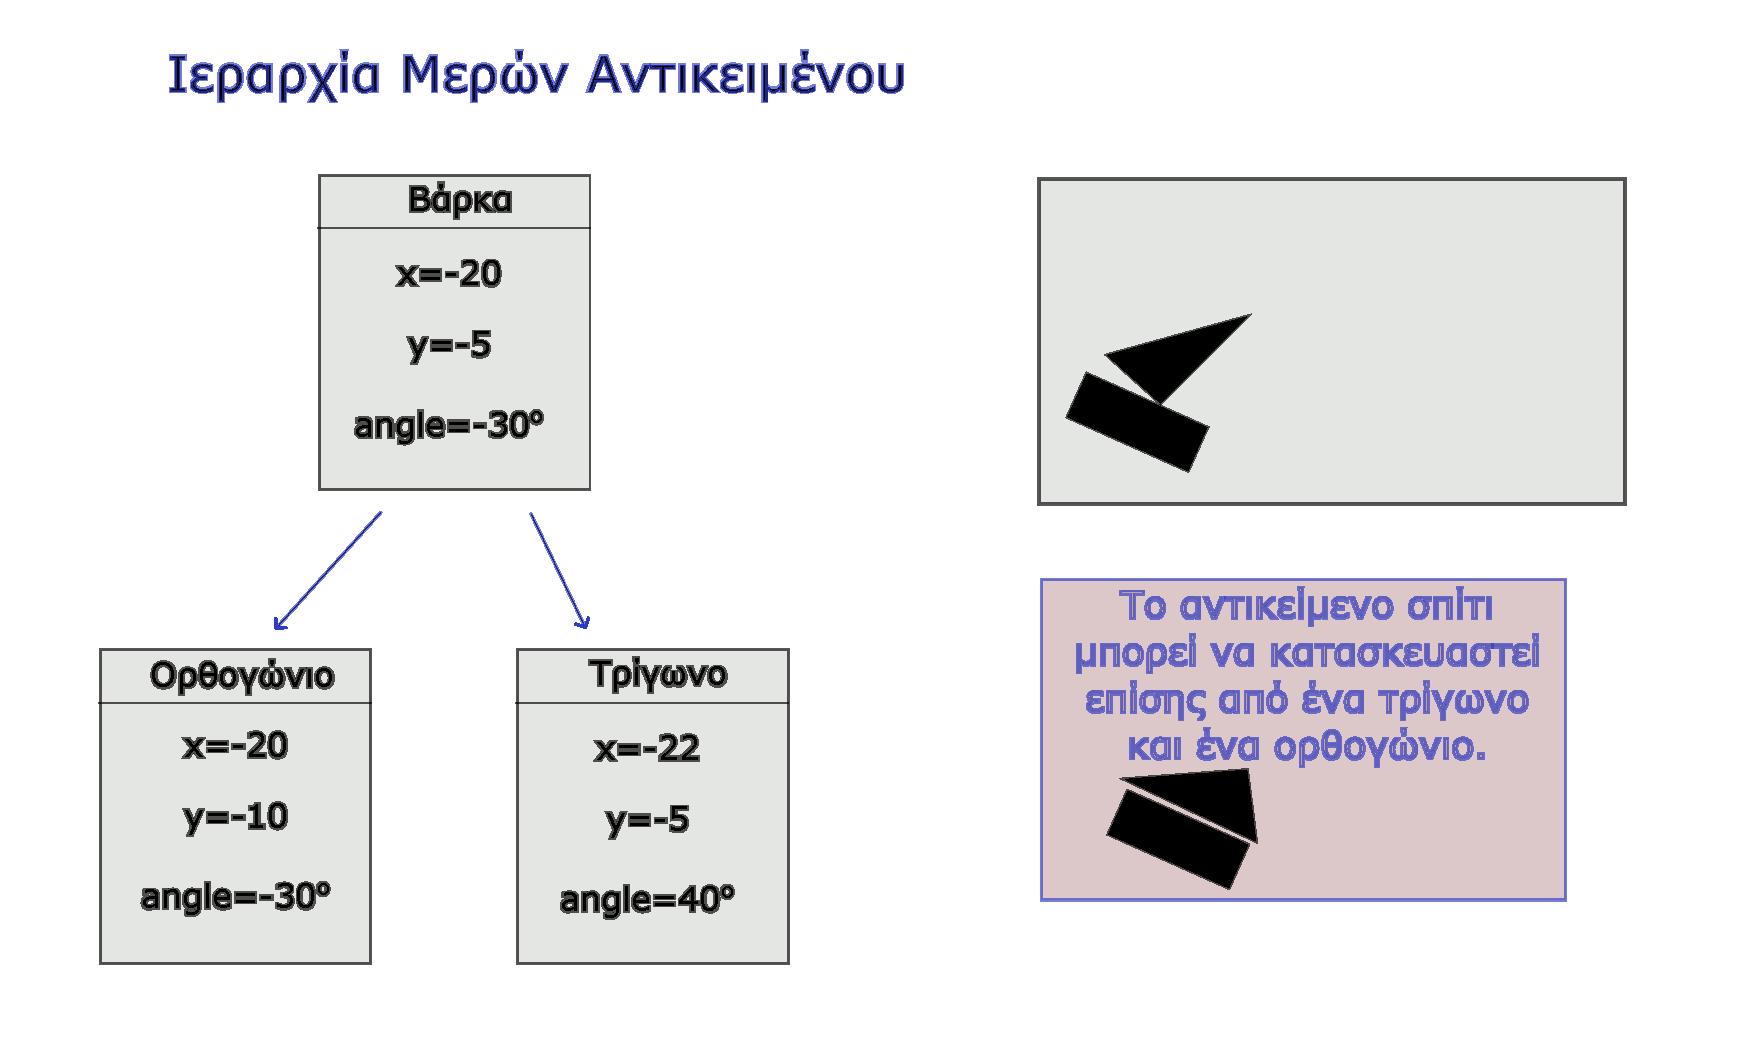
\includegraphics[width=0.8\textwidth]{images/chapter theoritical background/tree_of_objects_gr.pdf}
  \caption{Παρατηρούμε ότι με τα ίδια τμήματα μπορούμε να φτιάξουμε δύο διαφορετικά αντικείμενα (βάρκα και σπίτι). Παίζει μεγάλο ρόλο λοιπόν η σωστή αναγνώριση της γεωμετρίας των μερών και το πως συνδέονται αυτά μεταξύ τους. \textit{Παράχθηκε από το \href{https://inkscape.org/}{\en{Inkscape}}}.}
  \label{fig:caps_tree}
\end{figure}

Τώρα, καλούμαστε να υπολογίσουμε τις κάψουλες του επόμενου επιπέδου γνωρίζοντας τις τιμές του προηγούμενου επιπέδου, μια διαδικασία που έχουμε ονομάσει δρομολόγηση μέσω συμφωνίας. Με αυτόν τον τρόπο, θα υπολογίσουμε τις παραμέτρους στιγμιοτύπου πιο σύνθετων αντικειμένων (βλ. σχήμα \ref{fig:caps_tree}). Για τον σκοπό αυτό, κάθε κάψουλα του πρώτου επιπέδου, με βάση τις τιμές της, παράγει τόσες προβλέψεις όσες είναι οι κάψουλες του επόμενου επιπέδου που βλέπει. Ας υποθέσουμε ότι υπάρχουν δύο κάψουλες στο επόμενο επίπεδο: μια που αναπαριστά την οντότητα σπίτι και μια που αναπαριστά την οντότητα βάρκα. Όπως γίνεται κατανοητό στο σχήμα \ref{fig:caps_votes_example} η κάθε κάψουλα του πρώτου επιπέδου προβλέπει το διάνυσμα της κάψουλας που αναπαριστά το σπίτι και τη βάρκα με το να πολλαπλασιάζει τις τιμές της με τον αντίστοιχο πίνακα μετασχηματισμού $W_{ij}$. \par

\begin{figure}[p]
  \centering
  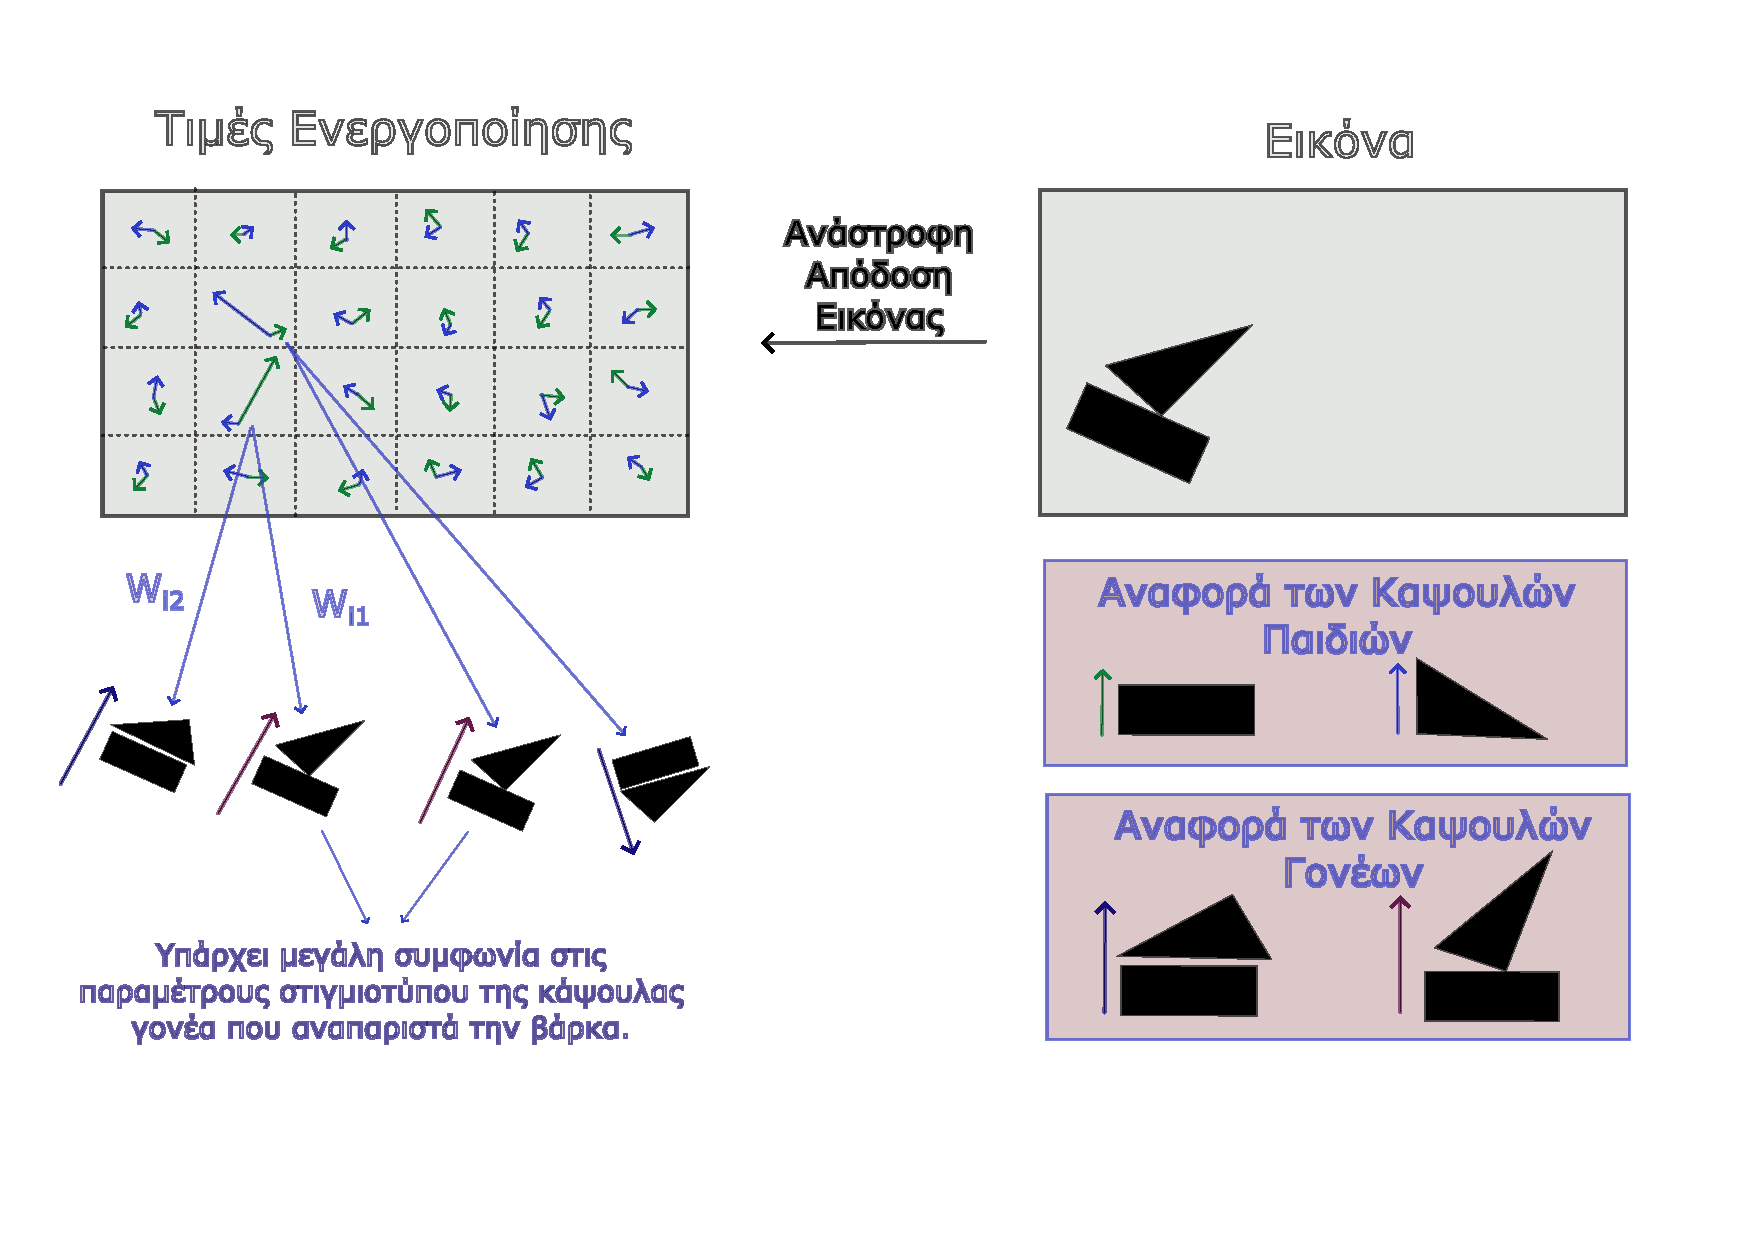
\includegraphics[width=0.8\textwidth]{images/chapter theoritical background/caps_votes_example_gr.pdf}
  \caption{Στο ανωτέρω σχήμα απεικονίζονται ενδεικτικά οι δύο προβλέψεις για τις δύο πιο ενεργές κάψουλες παιδιά (κάψουλες του προηγούμενου επιπέδου). Κάθε μια κάψουλα προσπαθεί να προβλέψει τη γεωμετρία των αντικειμένων του ανώτερου επιπέδου με βάση τη γεωμετρία της οντότητας που αναγνωρίζει. Βλέπουμε λοιπόν ότι το φιλτράρισμα συμπτώσεων υψηλής διάστασης είναι αποτελεσματικό αφού και οι δύο κάψουλες συμφωνούν στην οντότητα βάρκα. \textit{Παράχθηκε από το \href{https://inkscape.org/}{\en{Inkscape}}}.}
  \label{fig:caps_votes_example}
\end{figure}

Στην πρώτη επανάληψη του αλγορίθμου συμφωνίας, κάθε κάψουλα δρομολογεί στις κάψουλες ανώτερου επιπέδου τις προβλέψεις της ισάξια. Όμως, σύντομα αναγνωρίζεται ότι υπάρχει μεγάλη συμφωνία μεταξύ των προβλέψεων για βάρκα (βλ. σχήμα \ref{fig:caps_votes_example}). Λόγω της συμφωνίας, το διάνυσμα της κάψουλας για τη βάρκα που σχηματίζεται από τις σύμφωνες συστάδες προβλέψεων αποκτά μεγάλο μήκος. Έτσι, επαναληπτικά, οι κάψουλες προσαρμόζουν τα βάρη δρομολόγησης ώστε τελικά να δρομολογούν όλη την ψήφο τους στην οντότητα που τους εκφράζει καλύτερα (στην περίπτωσή μας, τη βάρκα).



\subsubsection{Υποθέσεις Νευρωνικών Δικτύων με Κάψουλες}
Οι υποθέσεις στις οποίες βασίζονται τα νευρωνικά δίκτυα με κάψουλες είναι οι εξής:
\begin{itemize}
  \item Οι τιμές των καψουλών ($M,a$) εξηγούν πιστά τις όποιες μεταβολές της εικόνας εισόδου και των αντικειμένων που αυτή περιέχει (\en{capturing equivariance}). Αντίθετα, οι πίνακες βαρών $W$ κωδικοποιούν την ανεξάρτητη (από την είσοδο) γνώση (\en{capturing invariance}).
  \item Οι πολυδιάστατες συμπτώσεις (\en{high\textendash dimensional coincidences}) αποτελούν ένα κατάλληλο φίλτρο για εξαγωγή χαρακτηριστικών.
  \item Αλλαγές στην οπτική γωνία προκαλούν μη γραμμικές μεταβολές στα εικονοστοιχεία και γραμμικές στις σχέσεις μεταξύ αντικειμένων (ή μερών του) και της κάμερας.
  \item Κάθε τμήμα ενός αντικειμένου ανήκει σε ένα γενικότερο αντικείμενο (\en{single parent assumption}) και κάθε περιοχή περιέχει το πολύ ένα στιγμιότυπο του ίδιου αντικειμένου\footnote{Η τελευταία υπόθεση είναι αναγκαία διότι στο ίδιο οπτικό πεδίο υπάρχει μια κάψουλα για κάθε οντότητα. Αυτό είναι και το τίμημα της χρήσης της θέσης των καψουλών μέσα στο δίκτυο για να προσδιοριστεί η ακριβής θέση των οντοτήτων που αναπαριστούν (όπως στα συνελικτικά νευρωνικά δίκτυα χωρίς επίπεδα συνάθροισης).}.
\end{itemize}

\subsubsection{Αδυναμίες των Νευρωνικών Δικτύων με Κάψουλες}
Αυτού του είδους των νευρωνικών δικτύων, ακόμα και στην πιο πρόσφατη υλοποίησή του από τον \en{G. Hinton}, παρουσιάζει ορισμένα προβλήματα. Αυτά, είναι τα εξής:
\begin{itemize}
  \item Δεν κλιμακώνονται εύκολα σε πιο μεγάλα και σύνθετα σύνολα δεδομένων λόγω υψηλών απαιτήσεων μνήμης και μη της έλλειψης αποδοτικών αλγορίθμων βελτιστοποιημένων ως προς τους υπολογισμούς ενός δικτύου με κάψουλες.
  \item Δεν είναι δυνατή η διαμόρφωση των πινάκων βαρών $W$ με μη\textendashεπιβλεπόμενη μάθηση (Κάτι τέτοιο θα συνέπτυσσε όλες τις ψήφους σε ένα σημείο.). ???? TODO
  \item Κάψουλες που αναπαριστούν αντικείμενα τα οποία λόγω της γεωμετρίας τους έχουν ακαθόριστη πόζα, δεν μπορούν να προβλέψουν τις παραμέτρους στιγμιοτύπου των επόμενων καψουλών. Για παράδειγμα, μια κάψουλα που αναπαριστά μια ρόδα δεν μπορεί να προβλέψει τη γεωμετρία του αυτοκινήτου.
  \item Είναι δύσκολη η παραμετροποίηση του αλγορίθμου εύρεσης συστάδων ώστε να επιτυγχάνεται υψηλή επίδοση. Η ρύθμιση του αλγορίθμου πρέπει να είναι τέτοια ώστε να πετυχαίνει μια ισορροπία μεταξύ της πυκνότητας των συστάδων και τον αριθμό των ψήφων που περιέχουν. 
\end{itemize}


\section{Μετασχηματιστές}

Σε αυτή την ενότητα θα αναφερθούμε σε μια αναδυόμενη αρχιτεκτονική νευρωνικών δικτύων, αυτή των Μετασχηματιστών (\en{Transformers}). Αν και αρχικά αναπτύχθηκε για εφαρμογές ακολουθιακών δεδομένων \cite{transformers_attention_is_all_you_need}, η μεγάλη της επιτυχία οδήγησε σύντομα στον πειραματισμό της με μη\textendash ακολουθιακά δεδομένα όπως αυτά των (στατικών) εικόνων \cite{dosovitskiy2020image_is_worth_16, carion2020_end_to_end_transformers}. Σε αυτήν την ενότητα θα κάνουμε μια σύντομη εισαγωγή στην τεχνολογία των επαναλαμβανόμενων νευρωνικών δικτύων (\en{Recurrent Neural Networks - RNNs})\cite{rumelhart1985learning_internal_representations} και σε ορισμένα προβλήματά της \cite{hochreiter1997lstm,bahdanau2014neural_machine_translation_attention_begins, transformers_attention_is_all_you_need}. Έπειτα, θα αναφερθούμε στις διαδοχικές βελτιώσεις - με κυριότερη αυτή της προσοχής (\en{attention})\cite{bahdanau2014neural_machine_translation_attention_begins} - οι οποίες τελικά διαμόρφωσαν την αρχιτεκτονική των μετασχηματιστών.

\subsection{Επαναλαμβανόμενα Νευρωνικά Δίκτυα}
Σε όλες τις αρχιτεκτονικές νευρωνικών δικτύων που έχουμε παρουσιάσει μέχρι τώρα, δε μας έχει απασχολήσει η σειρά με την οποία τροφοδοτούμε ένα σύστημα με τα παραδείγματα ενός συνόλου δεδομένων. Αυτό διότι έχουμε θεωρήσει ότι τα παραδείγματα εντός ενός συνόλου είναι διατεταγμένα με τυχαίο τρόπο, ανεξάρτητα μεταξύ τους\footnote{Η ιδιότητα της ανεξαρτησίας είναι η μία από τις δύο θεμελιώδεις υποθέσεις των συνόλων δεδομένων που χρησιμοποιούνται σε εφαρμογές μηχανικής μάθησης. Η δεύτερη υπόθεση είναι ότι όλα τα δείγματα ακολουθούν την ίδια κατανομή πιθανότητας.}. Στην εφαρμογή αναγνώρισης τροχοφώρων οχημάτων, για παράδειγμα, η ταξινόμηση μιας εικόνας σε ένα από τα είδη τροχοφόρων οχημάτων δε θα προσέδιδε καμία πληροφορία για την επόμενη προς ταξινόμηση εικόνα. Παρόλα αυτά, στα ακολουθιακά δεδομένα η ανεξαρτησία μεταξύ των δειγμάτων δεν ισχύει. Με άλλα λόγια, τα επιμέρους δείγματα συνδέονται μεταξύ τους έτσι ώστε η γνώση του ενός να προσδίδει πληροφορία για το άλλο. Μάλιστα, οι σχέσεις αυτές είναι συνήθως εντονότερες όταν η απόσταση μεταξύ των δειγμάτων στην ακολουθία είναι μικρή. Λόγου χάρη, στην ακολουθία τιμών θερμοκρασίας ενός δωματίου, όπως προκύπτει από την περιοδική μέτρηση ενός αισθητήρα, μπορεί κανείς να προβλέψει τη μελλοντική τιμή βασιζόμενος στις αμέσως προηγούμενες μετρήσεις. Σε γενικότερες γραμμές, όλες οι χρονοσειρές μπορούν να ενταχθούν στην κατηγορία των ακολουθιακών δεδομένων.\par

Η ύπαρξη τέτοιων ακολουθιακών δεδομένων προδιέθεσε την ανάπτυξη αρχιτεκτονικών νευρωνικών δικτύων που αναγνωρίζουν μοτίβα σε αυτά. Έτσι, γίνεται αξιοποίηση της κρυφής (\en{hidden}) πληροφορίας που αποκαλύπτουν οι μη\textendash ανεξάρτητες σχέσεις μεταξύ των δειγμάτων. Αν και ήδη από το 1943 οι \en{Warren McCulloch} και \en{Walter Pitts}\cite{mcculloch1943logical} περιέγραφαν την ιδέα ύπαρξης κυκλικών (επαναλαμβανόμενων) νευρωνικών δικτύων, αυτή άρχισε να λαμβάνει πρακτική υπόσταση υπό το όνομα \textquote{επαναληπτικά νευρωνικά δίκτυα} αργότερα, με τα έργα των \en{David E. Rumelhart et al.} \cite{rumelhart1985learning_internal_representations} και του \en{Michael I. Jordan} \cite{jordan1997serial}. \par

Σε μια πιο τυπική περιγραφή των επαναληπτικών νευρωνικών δικτύων, πρόκειται για το είδος αυτό που μπορεί να χειριστεί αποτελεσματικά ακολουθίες μεταβλητού μήκους\cite{geron2019hands}. Προκειμένου να το επιτύχει αυτό, απαιτείται ένας μηχανισμός ο οποίος θα αξιοποιεί τις σχέσεις αλληλεξάρτησης μεταξύ των επιμέρους δειγμάτων. Αυτό επιτυγχάνεται διαδίδοντας την πληροφορία που έχει εξαχθεί κατά την επεξεργασία των προηγούμενων δειγμάτων μιας ακολουθίας, στους κόμβους επεξεργασίας των επόμενων\cite{youtubeRNN}. Για αυτό τον λόγο, καταλήγουμε σε μια αρχιτεκτονική όπως αυτή ενός νευρωνικού δικτύου πρόσθιας τροφοδότησης αλλά με επιπλέον, ανάστροφες ακμές\cite{geron2019hands}. \par

\begin{figure}[h]
  \centering
  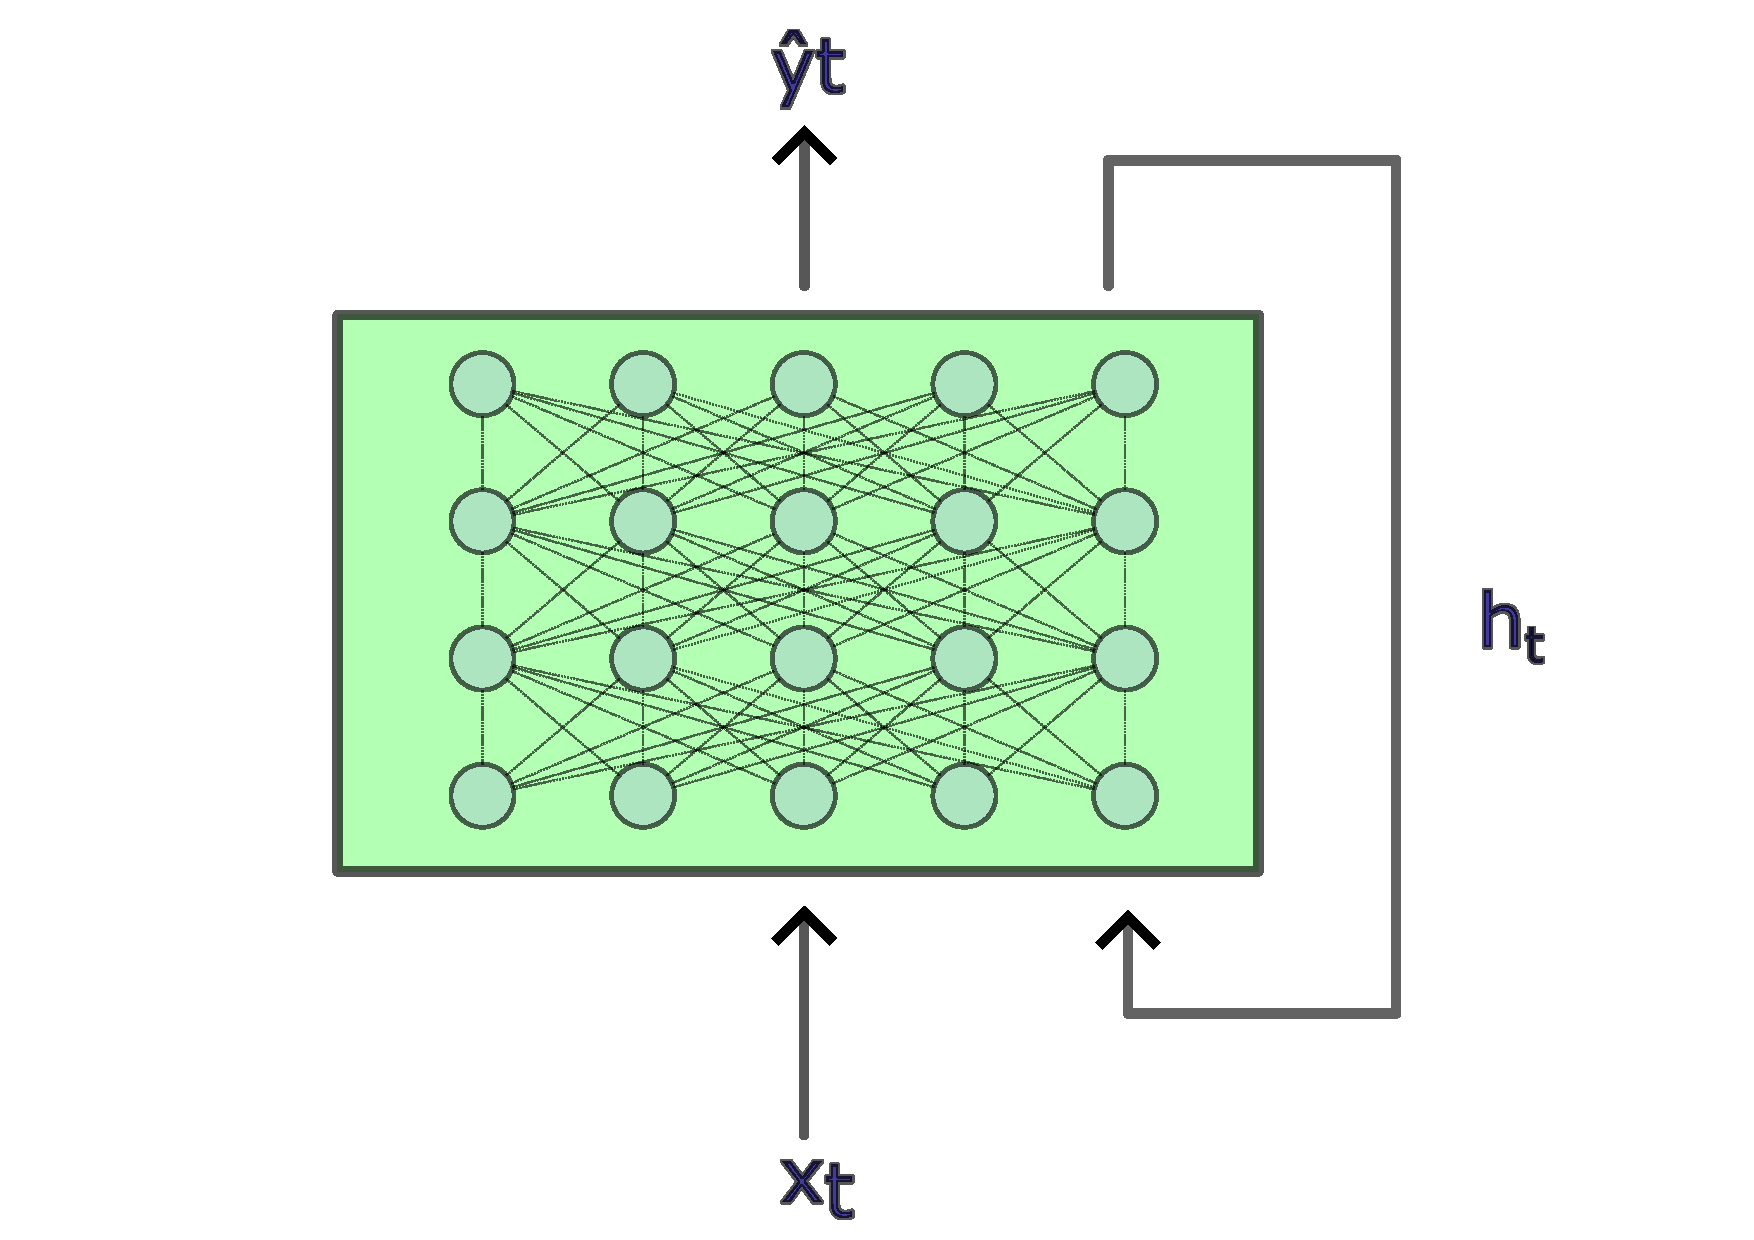
\includegraphics[width=0.6\textwidth]{images/chapter theoritical background/rnn_not unrolled.pdf}
  \caption{Στο ανωτέρω σχήμα απεικονίζονται η αρχιτεκτονική ενός επαναληπτικού νευρωνικού δικτύου. Το δίκτυο δέχεται ένα δείγμα ακολουθίας τη χρονική στιγμή $t$ και παράγει δύο εξόδους: την $\hat{y}_t$ και το διάνυσμα κρυφής κατάστασης $h_{t}$ (το οποίο και χρησιμοποιεί στην επόμενη χρονική στιγμή). \textit{Παράχθηκε από το \href{https://inkscape.org/}{\en{Inkscape}}}.}
  \label{fig:rnn_simple}
\end{figure}

Η αφαιρετική αρχιτεκτονική ενός επαναλητπικού νευρωνικού δικτύου φαίνεται στο σχήμα \ref{fig:rnn_simple}. Ας υποθέσουμε ότι στην είσοδο δίνεται ως παράδειγμα\footnote{Στο πλαίσιο των επαναληπτικών νευρωνικών δικτύων, με τον όρο παράδειγμα ενός συνόλου δεδομένων θα αναφερόμαστε σε μια ακολουθία από δείγματα.} μια ακολουθία $\underline{X} = [X_1, X_2, \dots, X_{T_x}]$ αποτελούμενη από $X_1, X_2, \dots, X_{T_x}$ επιμέρους δείγματα (όπου το καθένα αποτελείται από $d_{features}$ χαρακτηριστικά, δηλαδή: $X_i \in \Re^{d_{features}}$). Τότε, σειριακά, σε κάθε χρονικό βήμα (ή καρέ) $t$, το νευρωνικό δίκτυο θα δέχεται σαν είσοδο ένα δείγμα $X_t$ και θα παράγει μια έξοδο $\hat{y}_t$. Η πρακτική διαφοροποίηση με τα νευρωνικά δίκτυα πρόσθιας τροφοδότησης έγκειται στο ότι εκτός από αυτά τα διανύσματα, ένα επαναληπτικό νευρωνικό δίκτυο παράγει σε κάθε βήμα και μια δεύτερη έξοδο, το διάνυσμα κατάστασης $h_{t}$ το οποίο αποθηκεύει (σαν κυψέλη μνήμης) την πληροφορία των προηγούμενων δειγμάτων και τροφοδοτείται σαν είσοδο στο επόμενο καρέ (μέσω της ανάστροφης ακμής). Συνεπώς, στους υπολογισμούς του βήματος $t+1$, θα ληφθεί υπόψη όχι μόνο το παρόν δείγμα $X_{t+1}$ αλλά και η πρότερη χρήσιμη πληροφορία, κωδικοποιημένη στο διάνυσμα κατάστασης $h_{t}$\footnote{Το διάνυσμα $h_{t}$ θα μπορούσε στην απλούστερη περίπτωση να είναι ίδιο με το $\hat{y}_{t}$. Στις περισσότερες σύνθετες εφαρμογές όμως, παρατηρούνται οφέλη όταν τα διανύσματα αυτά είναι διαφορετικά.}. Τέλος, για λόγους κατανόησης θα εξυπηρετούσε να επισημάνουμε πως οι σειριακοί υπολογισμοί που προαναφέραμε μπορούν να \textquote{ξετυλιχτούν} στον χρόνο σχηματίζοντας το διάγραμμα \ref{fig:rnn_unrolled}.\par

\begin{figure}[h]
  \centering
  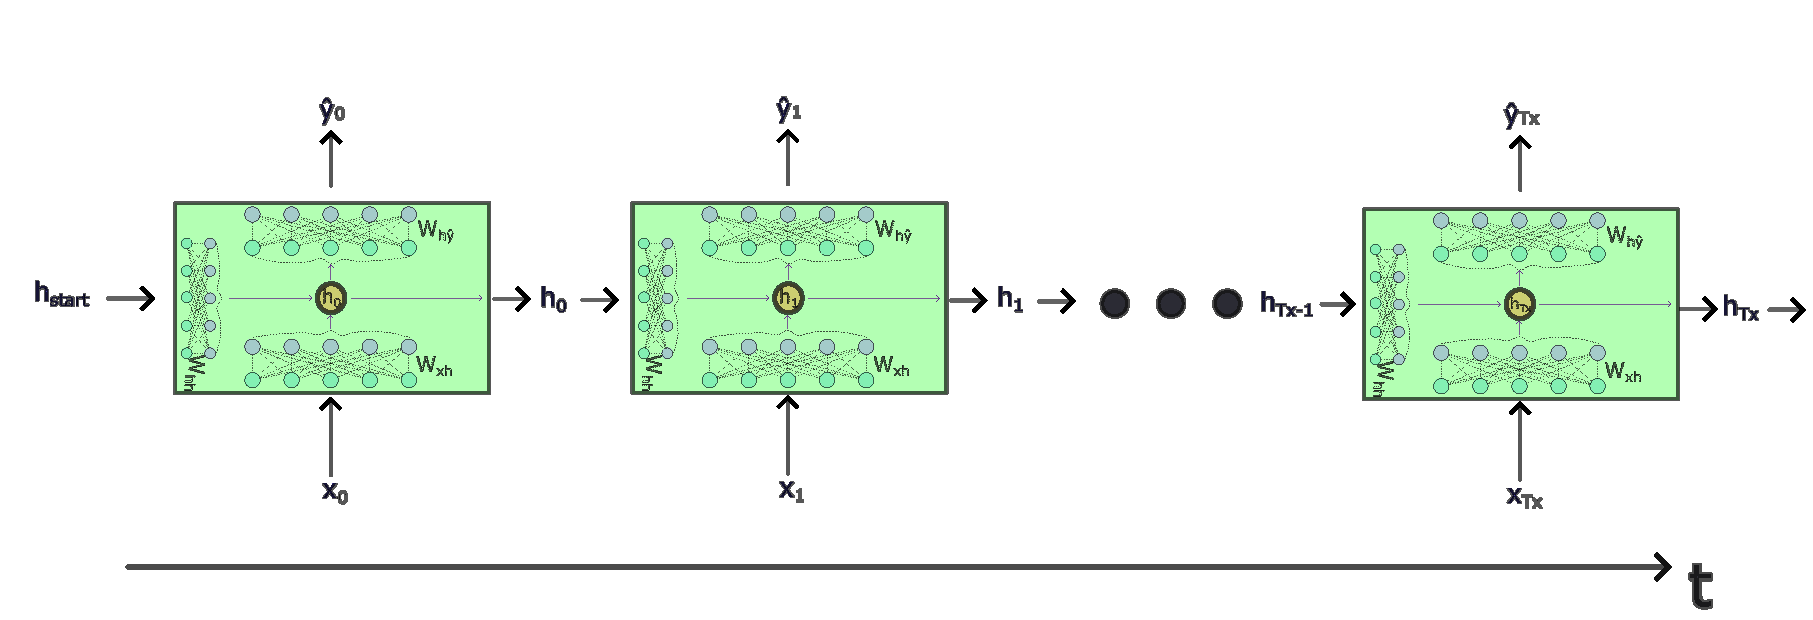
\includegraphics[width=0.95\textwidth]{images/chapter theoritical background/rnn_unroled.pdf}
  \caption{Στο ανωτέρω σχήμα απεικονίζεται η αρχιτεκτονική ενός επαναληπτικού νευρωνικού δικτύου \textquote{ξετυλιγμένου} στον χρόνο. Στην αρχή τροφοδοτούμε το δίκτυο με μια αρχική κρυφή κατάσταση (μπορεί να είναι τυχαία αρχικοποιημένη). Τροφοδοτούμε το δίκτυο με τα δείγματα της ακολουθίας εισόδου, ένα ανα χρονική στιγμή $t$ (στο σχήμα έχουμε υποθέσει ότι $d_{features} = 5$). Σε κάθε βήμα, μετακινούμαστε μια θέση δεξιά (στον άξονα του χρόνου). Να σημειώσουμε ότι με πράσινο χρώμα απεικονίζονται οι κόμβοι εισόδου ενώ με μοβ οι κόμβοι εξόδου. \textit{Παράχθηκε από το \href{https://inkscape.org/}{\en{Inkscape}}}.}
  \label{fig:rnn_unrolled}
\end{figure}


Με μαθηματικούς όρους, το διάνυσμα κατάστασης τη χρονική στιγμή $t$ προκύπτει ως συνάρτηση της προηγούμενης (κρυφής) κατάστασης και του δείγματος εισόδου, δηλαδή:
\begin{equation}
  h_t = f_{W_{h}}(x_t, h_{t-1}) = tanh(\boldsymbol{W_{hh}^T}\times h_{t-1}+\boldsymbol{W_{xh}^T}\times x_t) .
\end{equation}
Επιπλέον, για την έξοδο σε κάθε βήμα ισχύει:
\begin{equation}
  \label{eq:ytrnn}
  \hat{y}_{t} = f_{W_{\hat{y}}}(x_t, h_{t-1}) = \boldsymbol{W_{h\hat{y}}^T}\times h_t,
\end{equation} όπου το $h_t$ ενσωματώνει τα $x_t, h_{t-1}$.\par

Να σημειωθεί ότι οι παράμετροι των δύο συναρτήσεων, $f_{W_{\hat{y}}}$ και $f_{W_{h}}$, δε μεταβάλλονται ανάλογα με την ακολουθία εισόδου αλλά εκπαιδεύονται μέσω ενός τροποποιημένου αλγορίθμου οπίσθοδιάδοσης (οπισθοδιάδοση στο χρόνο - \en{Back Propagation Through Time}) έτσι ώστε τα βάρη και τα δυναμικά πόλωσης τους να λάβουν τιμές οι οποίες θα μοντελοποιούν καλύτερα τη σχέση εισόδου εξόδου. Η ενημέρωση των παραμέτρων πραγματοποιείται τουλάχιστον ανά $T_x$ χρονικές στιγμές. Η έννοια των συναρτήσεων $f_{W_{\hat{y}}}$ και $f_{W_{h}}$ είναι ίδια με την κλασσική περίπτωση νευρωνικού δικτύου όπου συμβολίζαμε τη συνάρτηση που αυτό μοντελοποιεί ως $\mathcal{F}(X;\overline{W},\overline{b}):X \rightarrow \hat{Y}$. Η διαφορά έγκειται ότι τώρα έχουμε δύο τέτοιες συναρτήσεις: μια που έχει ως έξοδο την επόμενη κρυφή κατάσταση $h$ και μια που έχει έξοδο την παρατηρήσιμη τιμή $\hat{y}$.\par

\begin{figure}[h]
  \centering
  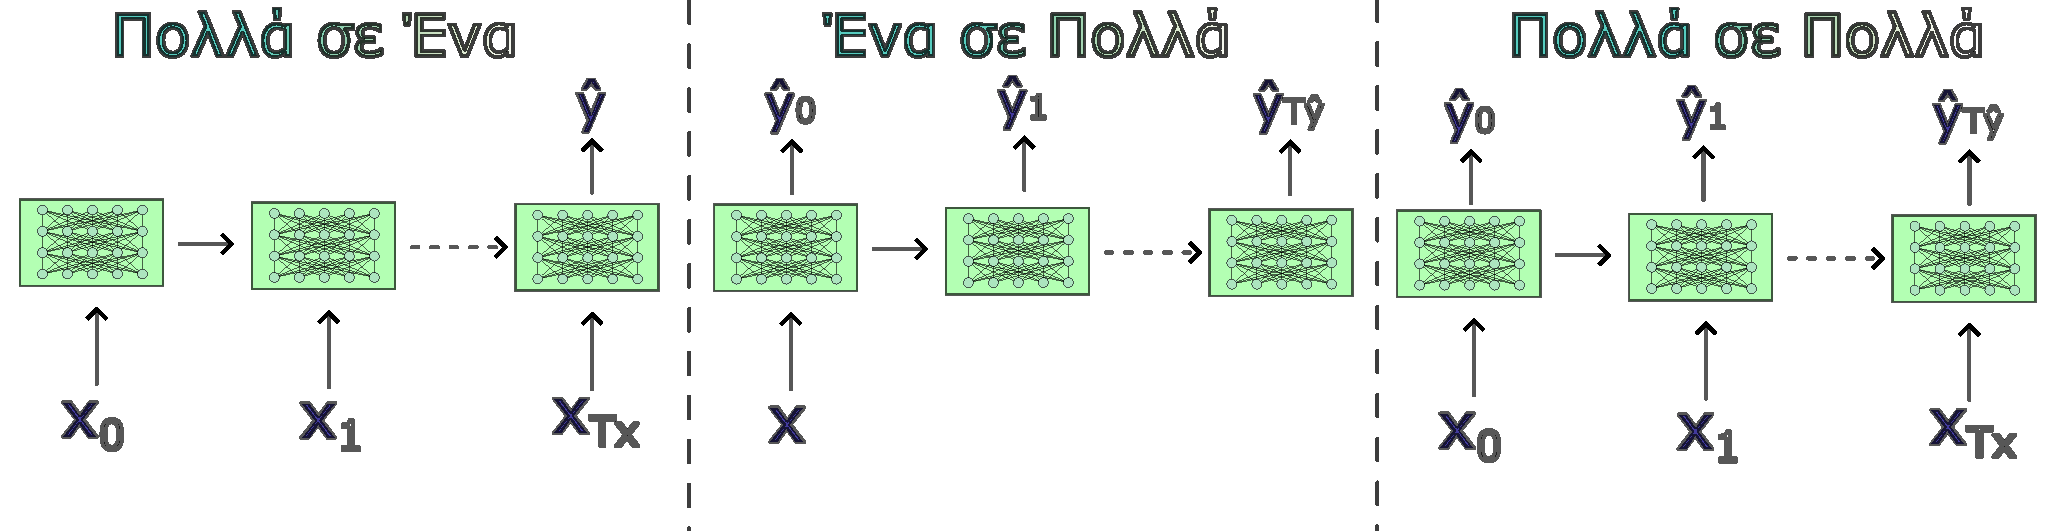
\includegraphics[width=0.92\textwidth]{images/chapter theoritical background/rnn_types_gr.pdf}
  \caption{Οι τρείς παραλλαγές επαναληπτικών νευρωνικών δικτύων ανάλογα με την είσοδο και την έξοδό τους. Σημειώνουμε ότι στην δεξιότερη παραλλαγή (Πολλά σε Πολλά) υποχρεωτικά με την απεικονιζόμενη αρχιτεκτονική ισχύει $T_x = T_{\hat{y}}$. \textit{Παράχθηκε από το \href{https://inkscape.org/}{\en{Inkscape}}}.}
  \label{fig:rnn_types}
\end{figure}

Υπάρχουν διάφορες παραλλαγές της αρχιτεκτονικής των επαναληπτικών νευρωνικών δικτύων ανάλογα με την εφαρμογή που διαχειρίζονται. Οι πιο βασικές κατηγορίες είναι οι εξής (βλ. σχήμα \ref{fig:rnn_types}):
\begin{itemize}
  \item Πολλά σε Ένα: Πρόκειται για το σύστημα που δέχεται σαν είσοδο μια ακολουθία και παράγει σαν έξοδο μια τιμή ή ένα διάνυσμα μη\textendash ακολουθιακού χαρακτήρα. Παράδειγμα εφαρμογής που απαιτεί αυτή την κατηγορία επαναληπτικών νευρωνικών δικτύων είναι η ταξινόμηση συναισθήματος (\en{sentiment classification}) όπου δοθέντος ενός κειμένου, καλείται παραδείγματος χάρη να το χαρακτηρίσει σαν θετικό, αρνητικό ή ουδέτερο.
  \item Ένα σε Πολλά: Σε αυτή την κατηγορία, η είσοδος δεν έχει ακολουθιακή οργάνωση αλλά η έξοδος έχει. Παράδειγμα εφαρμογής αποτελεί η αυτόματη παραγωγή λεζάντων σε εικόνες (μη\textendash ακολουθιακά δεδομένα).
  \item Πολλά σε Πολλά: Είναι ο μετασχηματισμός μιας ακολουθίας σε μια άλλη από μοντέλα τα οποία ονομάζονται γενικά \textquote{ακολουθία\textendash σε\textendash ακολουθία} (\en{seq2seq models}). Χαρακτηριστική εργασία που ανήκει σε αυτήν την κατηγορία είναι αυτή της μετάφρασης από μια γλώσσα σε μια άλλη.
\end{itemize}\par

\begin{figure}[h]
  \centering
  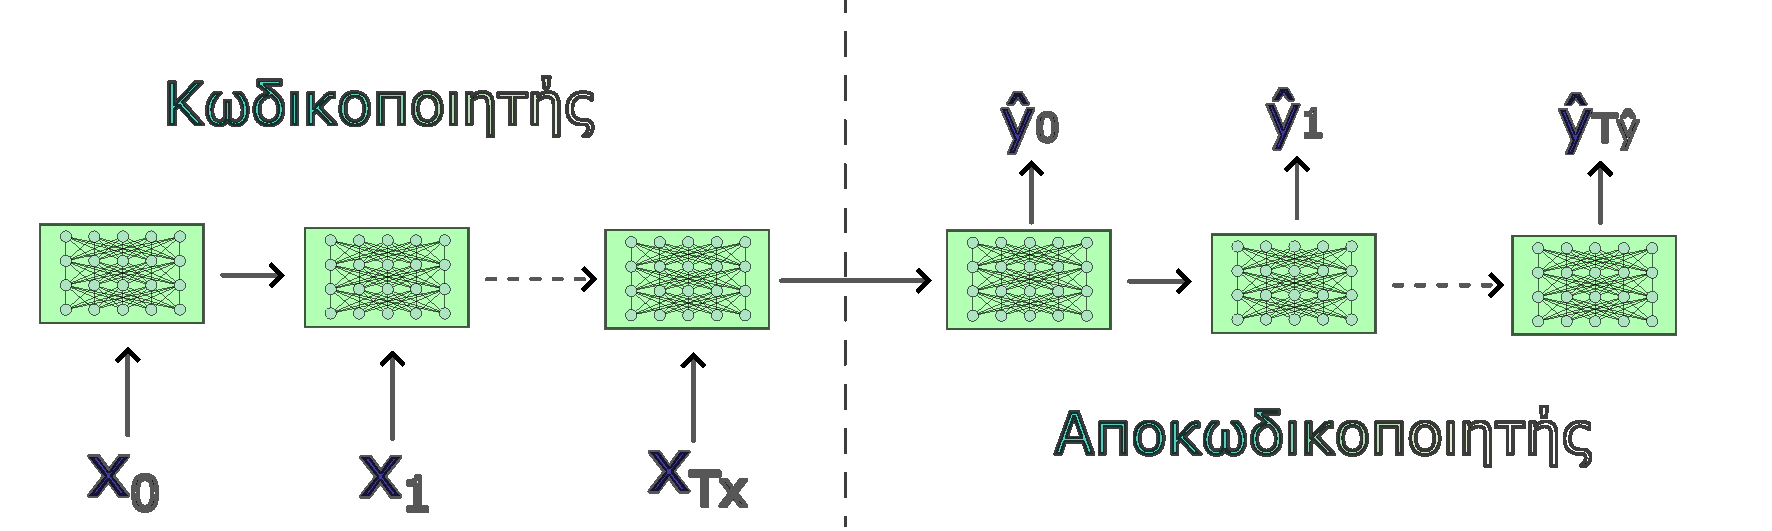
\includegraphics[width=0.8\textwidth]{images/chapter theoritical background/rnn_many_to_many_encoder_decoder_gr.pdf}
  \caption{Μια διαφορετική αρχιτεκτονική για την παραλλαγή \textquote{Πολλά σε Πολλά}. Ονομάζεται αρχιτεκτονική Κωδικοποιητή\textendash Αποκωδικοποιητή. Παρατηρούμε ότι όλη η γνώση της ακολουθίας εισόδου μεταφέρεται στον αποκωδικοποιητή μέσα από μια ακμή (ένα διάνυσμα κρυφής κατάστασης προκαθορισμένου μεγέθους). Σημειώνουμε ότι μπορεί να ισχύει $T_x \neq T_{\hat{y}}$. \textit{Παράχθηκε από το \href{https://inkscape.org/}{\en{Inkscape}}}.}
  \label{fig:rnn_enc_dec}
\end{figure}

Όλες οι εφαρμογές μοντελοποίησης ακολουθιών, ανεξάρτητα από τη λειτουργία τους, πρέπει να σχεδιάζονται έτσι ώστε να:
\begin{enumerate}
  \item Διαχειρίζονται ακολουθίες μεταβλητού μήκους. Δηλαδή οι ακολουθίες εισόδου $\underline{X} = [X_1, X_2, \dots, X_{T_{x}}]$ ή εξόδου $\underline{\hat{Y}} = [\hat{Y}_1, \hat{Y}_2, \dots, \hat{Y}_{T_{\hat{y}}}]$  που διαχειρίζεται το σύστημα να μην έχουν υποχρεωτικά όλες το ίδιο $T$\footnote{Υποχρεωτικά, κάθε δείγμα της ακολουθίας εισόδου (και εξόδου, αντίστοιχα) κωδικοποιείται με τον ίδιο αριθμό χαρακτηριστικών ($d_{features}$), δηλαδή: $X_i \in \Re^{d_{{features}_X}}, \forall i \in [1, T_{x}]$ και $\hat{Y}_i \in \Re^{d_{{features}_{\hat{Y}}}}, \forall i \in [1, T_{\hat{y}}]$}.
  \item Ανιχνεύουν εξαρτήσεις μεταξύ δειγμάτων στην ακολουθία που μπορεί να έχουν μεγάλη απόσταση μεταξύ τους.
  \item Διατηρούν την πληροφορία σχετικά με τη σειρά των στοιχείων στην ακολουθία. Αυτό έχει πρωτεύουσα σημασία σε τέτοιες εφαρμογές αφού για παράδειγμα, η αλλαγή της σειράς των λέξεων σε μια πρόταση μπορεί να αλλάξει ριζικά την ερμηνεία της.
  \item Διαμοιράζονται παραμέτρους μεταξύ των χρονικών στιγμών (π.χ. μέσω διανυσμάτων καταστάσεων $h$) ώστε να μπορούν να εντοπίζουν μακρινές εξαρτήσεις. \cite{youtubeRNN}
\end{enumerate}

\subsubsection{Προβλήματα Επαναλαμβανώμενων Νευρωνικών Δικτύων}
Τα επαναληπτικά νευρωνικά δίκτυα, στην απλή τους μορφή που παρουσιάσαμε, μπορούν και πληρούν επαρκώς τα ανωτέρω κριτήρια σε απλές εφαρμογές. Παρόλλα αυτά, σε πιο σύνθετες εφαρμογές δημιουργούνται ορισμένα προβλήματα. Η κύρια πηγή αυτών των προβλημάτων είναι το μεγάλο μήκος των ακολουθιών που καλούνται τα επαναληπτικά νευρωνικά δίκτυα να μοντελοποιήσουν.\par

\begin{figure}[h]
  \centering
  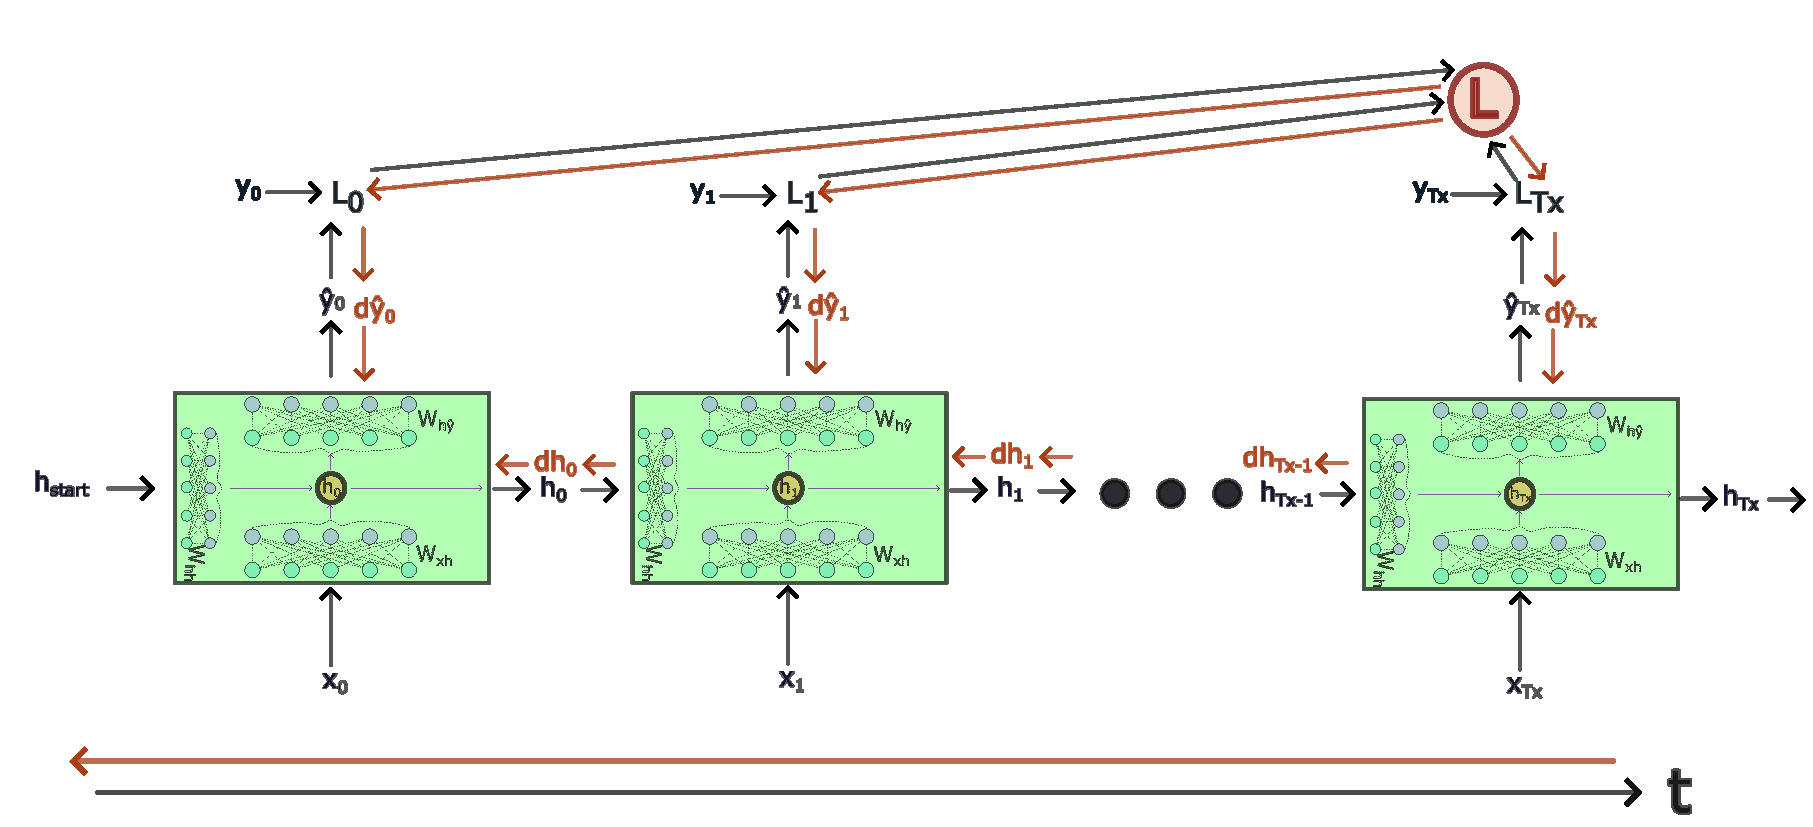
\includegraphics[width=0.95\textwidth]{images/chapter theoritical background/rnn_unroled_BPTT.pdf}
  \caption{Σχήμα στο οποίο απεικονίζεται η οπισθοδιάδοση του σφάλματος στον χρόνο (\en{Back Propagation Through Time}). Με γκρι βέλη απεικονίζεται η πρόσθια διάδοση για τον υπολογισμό της συνάρτησης απώλειας ενώ με κόκκινα βέλη η οπισθοδιάδοση (η οποία συμβαίνει αφού έχουν υπολογιστεί όλα τα $\hat{y}$ για την συγκεκριμένη ακολουθία εξόδου). \textit{Παράχθηκε από το \href{https://inkscape.org/}{\en{Inkscape}}}.}
  \label{fig:rnn_bptt}
\end{figure}

Το πρώτο πρόβλημα είναι αυτό των εξαφανιζόμενων ή εκρηγνόμενων κλίσεων (\en{vanishing/exploding gradients}). Σε αδρές γραμμές, όπως φαίνεται και στο σχήμα \ref{fig:rnn_bptt}, οι μερικές παράγογοι του σφάλματος ως προς τις παραμέτρους διαδίδονται μέσω του αλγορίθμου οπίσθοδιάδωσης κλίσης όχι μόνο στον εγκάρσιο άξονα εισόδου\textemdash εξόδου αλλά και στον διαμήκη άξονα του χρόνου από το τελευταίο καρέ στο πρώτο. Έτσι, αν οι ιδιοτιμές $\lambda$ του πίνακα $\boldsymbol{W_{hh}}$ είναι λίγο μεγαλύτερες της μονάδος, οι διαδοχικοί πολλαπλασιασμοί του σφάλματος με την ποσότητα $\boldsymbol{W_{hh}}$ για τον υπολογισμό της κλίσης ως προς τις παραμέτρους στα αρχικά καρέ θα διογκώσει το σφάλμα κατά ${\lambda}^{T}$ οδηγώντας στην υπερχείλιση (\en{overflow}). Αντίστοιχα, στην περίπτωση που οι ιδιοτιμές είναι μικρότερες της μονάδος, έχουμε υποχείλιση (\en{underflow}). Επειδή λοιπόν το σφάλμα αδυνατεί να διαδοθεί στα πρώτα καρέ μακρυνών ακολουθιών, το δίκτυο αδυνατεί να αξιοποιήσει εξαρτήσεις που έχουν μεγάλη απόσταση μεταύ τους. Για παράδειγμα, ένα σύστημα πρόβλεψης επόμενης λέξης υλοποιημένο με ένα απλό επαναληπτικό νευρωνικό δίκτυο (\en{vanilla RNN}) θα αδυνατούσε να μεταφράσει την πρόταση \textquote{Μεγάλωσα στην Ελλάδα, ... άρα μιλάω άπταιστα <θέση-λέξης-για-πρόβλεψη>.} αν μεταξύ της λέξης \textquote{Ελλάδα} και της πρόβλεψης παρεμβάλονταν πολλές λέξεις. \par

\begin{figure}[h]
  \centering
  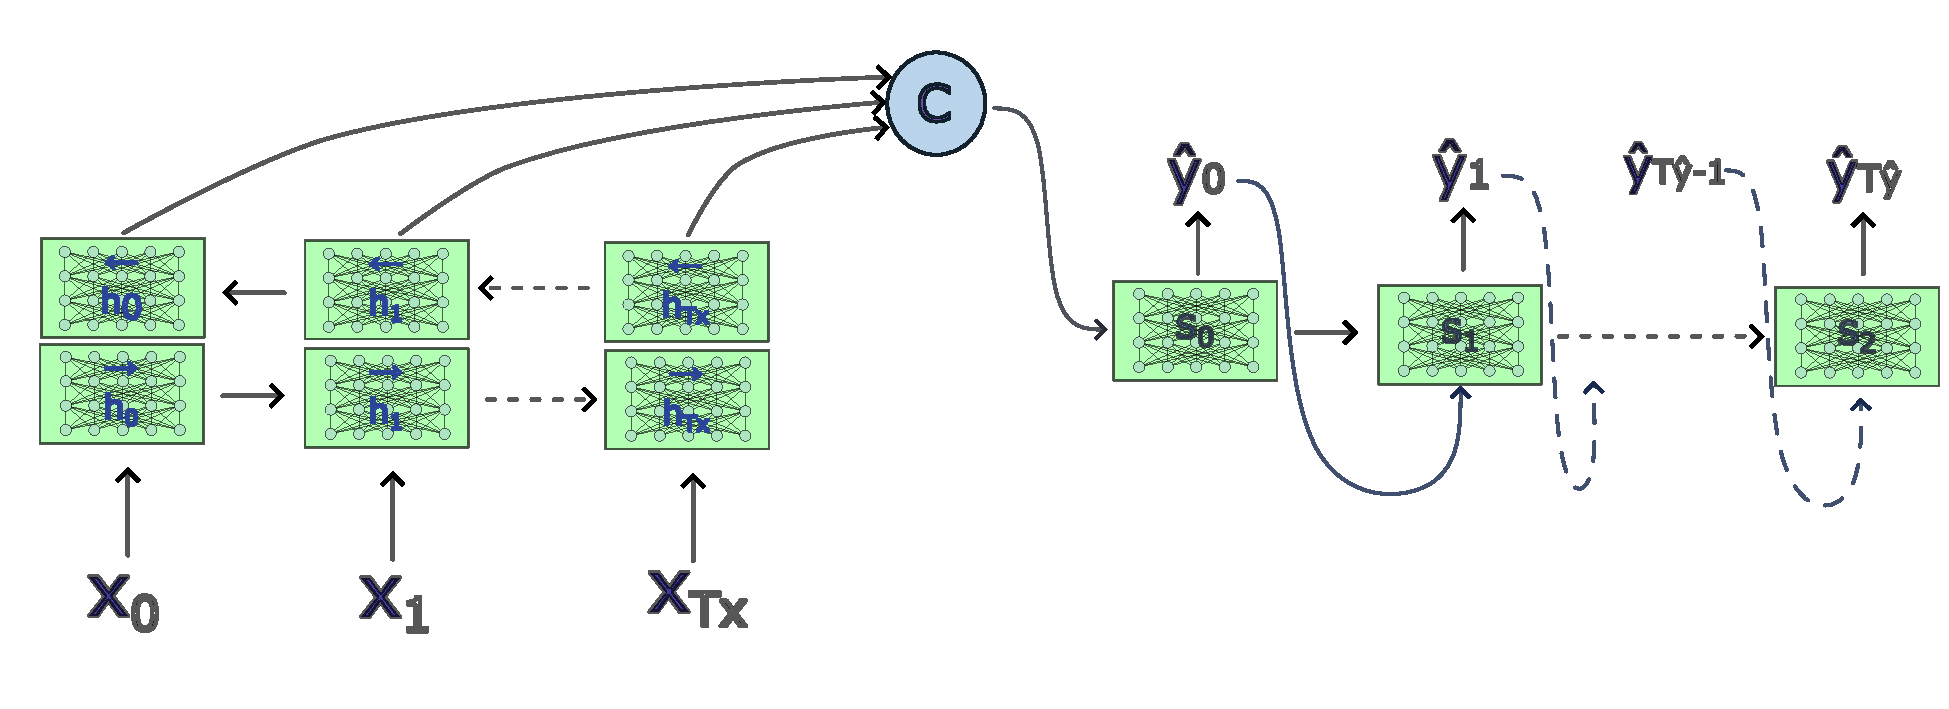
\includegraphics[width=0.95\textwidth]{images/chapter theoritical background/rnn_encoder_decoder_complex.pdf}
  \caption{Σχήμα στο οποίο απεικονίζεται μια πιο σύνθετη αρχιτεκτονική ενός επαναληπτικού νευρωνικού δικτύου τύπου κωδικοποιητή\textendash αποκωδικοποιητή. Σε αυτό, το διάνυσμα (\en{context}) που κωδικοποιεί την πληροφορία της ακολουθίας εισόδου σχηματίζεται από τις κρυφές καταστάσεις όλων των προηγούμενων δειγμάτων. Ο κωδικοποιητής αποτελείται από δύο επίπεδα επαναληπτικών δικτύων (ένα που δέχεται την ακολουθία με την χρονική σειρά και ένα με την ανάποδη). Η αρχιτεκτονική αυτή του κωδικοποιητή ονομάζεται \textquote{αμφίδρομο επαναληπτικό νευρωνικό δίκτυο} (\en{Bidirectional RNN}). Ο αποκωδικοποιητής αποτελεί ένα μοντέλο αυτοπαλινδρόμησης αφού η (κύρια) έξοδός του τροφοδοτείται αυτούσια σε μια από τις εισόδους για να χρησιμοποιηθεί την επόμενη χρονική στιγμή. \textit{Παράχθηκε από το \href{https://inkscape.org/}{\en{Inkscape}}}.}
  \label{fig:rnn_encoder_decoder_no_attention}
\end{figure}

Το δεύτερο πρόβλημα αφορά κυρίως τα επαναληπτικά νευρωνικά δίκτυα τύπου \textquote{ακολουθία\textendash σε\textendash ακολουθία} και δη αυτά σε μορφή κωδικοποιητή\textendash αποκωδικοποιητή (βλ. σχήμα \ref{fig:rnn_enc_dec} και σχήμα \ref{fig:rnn_encoder_decoder_no_attention}). Σε αυτά τα δίκτυα, ο κωδικοποιητής διαβάζει την ακολουθία εισόδου και σχηματίζει ένα διάνυσμα κατάστασης προκαθορισμένου μήκους το οποίο ενσωματώνει την πληροφορία αυτή. Στην συνέχεια, ο αποκωδικοποιητής λαμβάνει αυτό το διάνυσμα ως μοναδική είσοδο και παράγει την ακολουθία εξόδου. Έχει όμως δειχθεί ότι η επίδωση ενός τέτοιου συστήματος μειώνεται σημαντικά με την αύξηση του μήκους της ακολουθίας εισόδου \cite{cho2014properties}. Θα μπορούσαμε να ισχυριστούμε ότι η μείωση της επίδοσης οφείλεται στην συμφόριση (\en{bottleneck}) που προκαλείται με την απαίτηση ότι όλη η πληροφορία της ακολουθίας εισόδου να κωδικοποιείται σε ένα σταθερού\textendash μήκους διάνυσμα κατάστασης\cite{bahdanau2014neural_machine_translation_attention_begins}.\par

Το τρίτο πρόβλημα που γίνεται όλο και πιο έντονο σε σύνθετες εφαρμογές με μεγάλες ακολουθίες είναι οι αργοί χρόνοι εκπαίδευσης και πρόβλεψης. Τα επαναληπτικά νευρωνικά δίκτυα είναι σειριακής φύσεως με αποτέλεσμα να μην μπορεί να τροφοδοτηθεί κάθε δείγμα της ακολουθίας παράλληλα. Αντίθετα, για να τροφοδοτηθεί το επόμενο στην σειρά δείγμα θα πρέπει να έχει ολοκληρωθεί η επεξεργασία του προηγούμενου. Αυτό, αν και δεν είναι σοβαρό πρόβλημα σε απλές εφαρμογές με μικρό υπολογιστικό κόστος και μικρού μήκους ακολουθίες αποτελεί ένα ανυπέρβλητο εμπόδιο στην εκπαίδευση σύνθετων εφαρμογών που μοντελοποιούν ακολουθίες με εκτατοντάδες δείγματα η κάθε μια.

\subsubsection{Λύσεις στα Προβλήματα Επαναλαμβανώμενων Νευρωνικών Δικτύων}

Έχουν αναπτυχθεί διάφορες τεχνικές για την μετρίαση των ανωτέρω προβλήμάτων. Ενδεικτικά, για το πρόβλημα της υπερχείλισης ενδείκνεται η περικοπή της μεγάλης τιμής (σε ένα μικρότερο νούμερο) ώστε να μπορεί να αποθηκευθεί στον χώρο μνήμης που έχει διατεθεί για αυτή\cite{youtubeRNN}. Ανάλογα, για το πρόβλημα της υποχείλισης, αυτό βελτιώνεται με καλύτερη επιλογή συνάρτησης ενεργοποίησης και με προσεκτικότερη αρχικοποίηση των πινάκων βαρών\cite{youtubeRNN}. Τέλος, και για τις δύο υποπεριπτώσεις, μια νέα αρχιτεκτονική επαναληπτικών νευρωνικών δικτύων με όνομα Μακροπρόθεσμη\textendash Βραχυπρόθεσμη Μνήμη (\en{Long\textendash Short Term Memory - LSTM})\cite{hochreiter1997lstm} μπορεί να αυξήσει σημαντικά το μήκος των ακολουθιών που μπορεί ένα τέτοιο είδος δικτύου να διαχειριστεί\footnote{Η λύση αυτή δεν αποτελεί πανάκεια καθώς δεν εξαλείφει το πρόβλημα και επίσης με αυτή δεν μπορεί να γίνει μεταφορά γνώσης (\en{transfer learning})\cite{youtubeRNNleo}.}.\par

Σε ό,τι αφορά το πρόβλημα της συμφώρισης της κωδικοποιημένης πληροφορίας, έχει προταθεί η ενίσχυση των επαναληπτικών νευρωνικών δικτύων με έναν μηχανισμό προσοχής (\en{attention mechanism}) \cite{rumelhart1985learning_internal_representations}. Όπως θα αναλύσουμε στην συνέχεια, αυτός ο μηχανισμός επιτρέπει στον αποκωδικοποιητή επιλεκτικά, σε κάθε βήμα, να βλέπει τις προηγούμενες κρυφές καταστάσεις που θεωρεί πιο χρήσιμες για τον υπολογισμό της εξόδου στο βήμα αυτό\footnote{Η λύση αυτή μπορεί να συνδειαστεί με την αρχιτεκτονική επαναληπτικών νευρωνικών δικτύων \textquote{Μακροπρόθεσμης \textendash Βραχυπρόθεσμης Μνήμης}.}. \par

Αναζητώντας λύση για το τρίτο πρόβλημα, η επιστημονική κοινότητα, αντλώντας στοιχεία από τον μηχανισμό προσοχής, οδηγήθηκε σε μια εξ'ολοκλήρου νέα αρχιτεκτονική που διαφέρει από τα επαναληπτικά νευρωνικά δίκτυα. Αυτή ονομάζεται μετασχηματιστές (\en{transformers})\cite{transformers_attention_is_all_you_need} και όπως θα περιγράψουμε στην συνέχεια, τα δείγματα σε κάθε ακολουθία δεν τροφοδοτούνται στο μοντέλο σειριακά αλλά παράλληλα. Επιπλέον, μπορεί να κλιμακώσει εύκολα με αποτέλεσμα να δύναται να μοντελοποιεί μεγάλες σε μήκος ακολουθίες με μακρυνές εξαρτήσεις.\par

\subsection{Μηχανισμός Προσοχής}
Αν και ο μηχανισμός προσοχής έχει αποβεί χρήσιμος σε μια πληθόρα από εφαρμογές, αρχικά αναπτύχθηκε στο πλαίσιο του επαναληπτικού νευρωνικού δικτύου τύπου κωδικοποιητή\textendash αποκωδικοποιητή για να λύσει το πρόβλημα της συμφώρισης σε εφαρμογές μεταφράσεων. Η γενική ιδέα είναι ότι για τον υπολογισμό της εξόδου $\hat{y}_t$, κρίνεται σκόπιμο το δίκτυο να μπορεί να εστιάσει την προσοχή του σε συγκεκριμένα δείγματα εισόδου που θεωρεί πιο σχετικά. Τα δείγματα αυτά θα διαφέρουν από καρέ σε καρέ αφού διαφορετικές λέξεις εξόδου συσχετίζονται με διαφορετικές λέξεις εισόδου.\par

\begin{figure}[h]
  \centering
  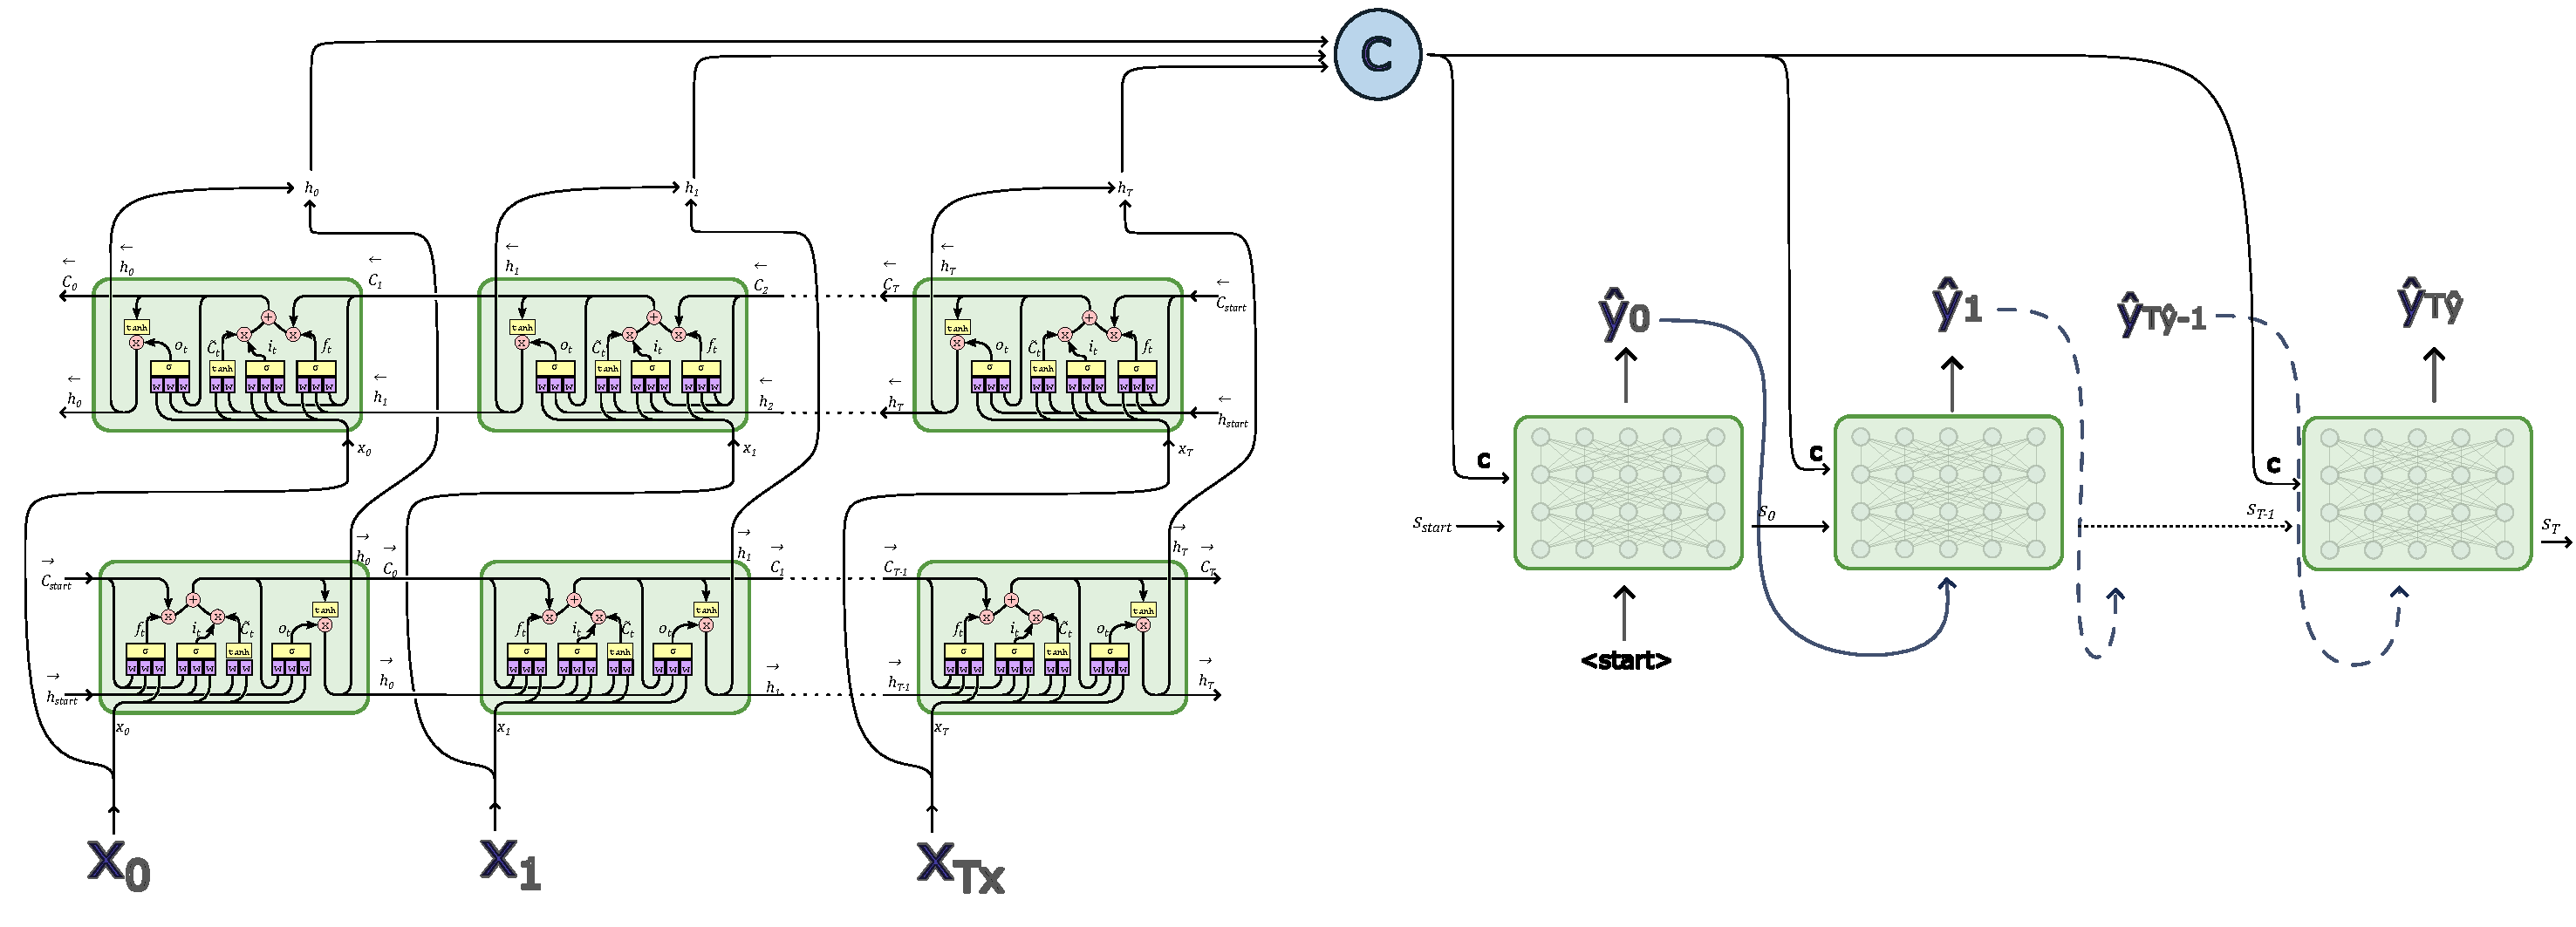
\includegraphics[width=0.95\textwidth]{images/chapter theoritical background/rnn_peaky_encoder_decoder_complex.pdf}
  \caption{Σχήμα στο οποίο απεικονίζεται μια ακόμα σύνθετη αρχιτεκτονική ενός επαναληπτικού νευρωνικού δικτύου τύπου κωδικοποιητή\textendash αποκωδικοποιητή (\en{peaky encoder-decoder}). Σε αυτό, το διάνυσμα (\en{context}) που κωδικοποιεί την πληροφορία της ακολουθίας εισόδου σχηματίζεται από τις κρυφές καταστάσεις όλων των προηγούμενων δειγμάτων και είναι ορατό σε κάθε βήμα τοη αποκωδικοποιητή. Η αρχιτεκτονική του κωδικοποιητή ονομάζεται \textquote{αμφίδρομο επαναληπτικό νευρωνικό δίκτυο από μονάδες Μακροπρόθεσμης\textendash Βραχυπρόθεσμης Μνήμης} (\en{Bidirectional LSTM}). Ο αποκωδικοποιητής μπορεί και αυτός να κατασκευάζεται από τροποποιημένες μονάδες Μακροπρόθεσμης\textendash Βραχυπρόθεσμης Μνήμης που θα ενσωματώνουν πλήρως διασυνδεδεμένα επίπεδα για τον υπολογισμό της εξόδου από τα διανύσματα κατάστασης. \textit{Παράχθηκε από το \href{https://inkscape.org/}{\en{Inkscape}}}.}
  \label{fig:rnn_peaky_encoder_decoder_no_attention}
\end{figure}

Στο σχήμα \ref{fig:rnn_peaky_encoder_decoder_no_attention} φαίνεται αναλυτικά ένα τέτοιο σύστημα χωρίς τον μηχανισμό προσοχής. Παρατηρούμε ότι ο κωδικοποιητής αποτελείται από δύο επαναληπτικά νευρωνικά δίκτυα: ένα με δεξιά κατεύθυνση και ένα με την αντίθετη κατεύθυνση, στοιβαγμένα το ένα πάνω στο άλλο\footnote{Η αρχιτεκτονική αυτή ονομάζεται αμφίδρομο επαναληπτικό νευρωνικό δίκτυο (\en{bidirectional recurrent neural network}).}\cite{schuster1997bidirectional}. Το κάθε ένα παράγει ένα διάνυσμα κατάστασης ($\overrightarrow{h}_t$ και $\overleftarrow{h}_t$ αντίστοιχα) σε κάθε καρέ τα οποία μετά τα ενώνουμε (\en{concatenate}) δηλαδή 
\[h_t = 
  \begin{bmatrix}
    \overrightarrow{h}_t\\
    \overleftarrow{h}_t
  \end{bmatrix}
.\]
Αυτό γίνεται επειδή επιθυμούμε το διάνυσμα κατάστασης σε κάθε σημείο να ενσωματώνει τόσο την πληροφορία για τα προηγούμενα δείγματα ($\overrightarrow{h}_t$) όσο και την πληροφορία για τα επόμενα ($\overleftarrow{h}_t$) \cite{bahdanau2014neural_machine_translation_attention_begins}. Μετά την δημιουργία των διανυσμάτων κατάστασης, αυτά χρησιμεύουν για την κατασκευή ενός διανύσματος συμφραόμενων (\en{context vector}) σταθερού μήκους το οποιο συμπυκνώνει\footnote{Η συμπύκνωση προκαλεί απώλεια  πληροφορίας που δημιουργεί το πρόβλημα της συμφόρησης.} την πληροφορία από όλα τα διανύσματα κατάστασης Δηλαδή:
\[
  c = q({h_1, h_2, \dots, h_{T_x}})
\]
όπου $q$ μια μη\textendash γραμμική συνάρτηση. Τέλος, ο αποκωδικοποιητής (όπως περιγράφεται από τους \en{Bahdanau D. et al.} \cite{bahdanau2014neural_machine_translation_attention_begins}) λαμβάνει σε κάθε βήμα την προηγούμενη πρόβλεψη $\hat{y}_{t-1}$, την προηγούμενη κατάσταση που στον αποκωδικοποιητή συμβολίεται με $s_{t-t}$ και το διάνυσμα συμφραζόμενων $c$ για να εξάγει την κατάσταση $s_t$. Δηλαδή, είναι:
\[
  s_t = f(s_{t-1}, y_{t-1}, c)
\]
Έπειτα, με αντίστοιχο τρόπο όπως παρουσιάσαμε με τη σχέση \ref{eq:ytrnn}, υπολογίζουμε την πρόβλεψη $y_t$ από το διάνυσμα $s_t$.\par

\begin{figure}[h]
  \centering
  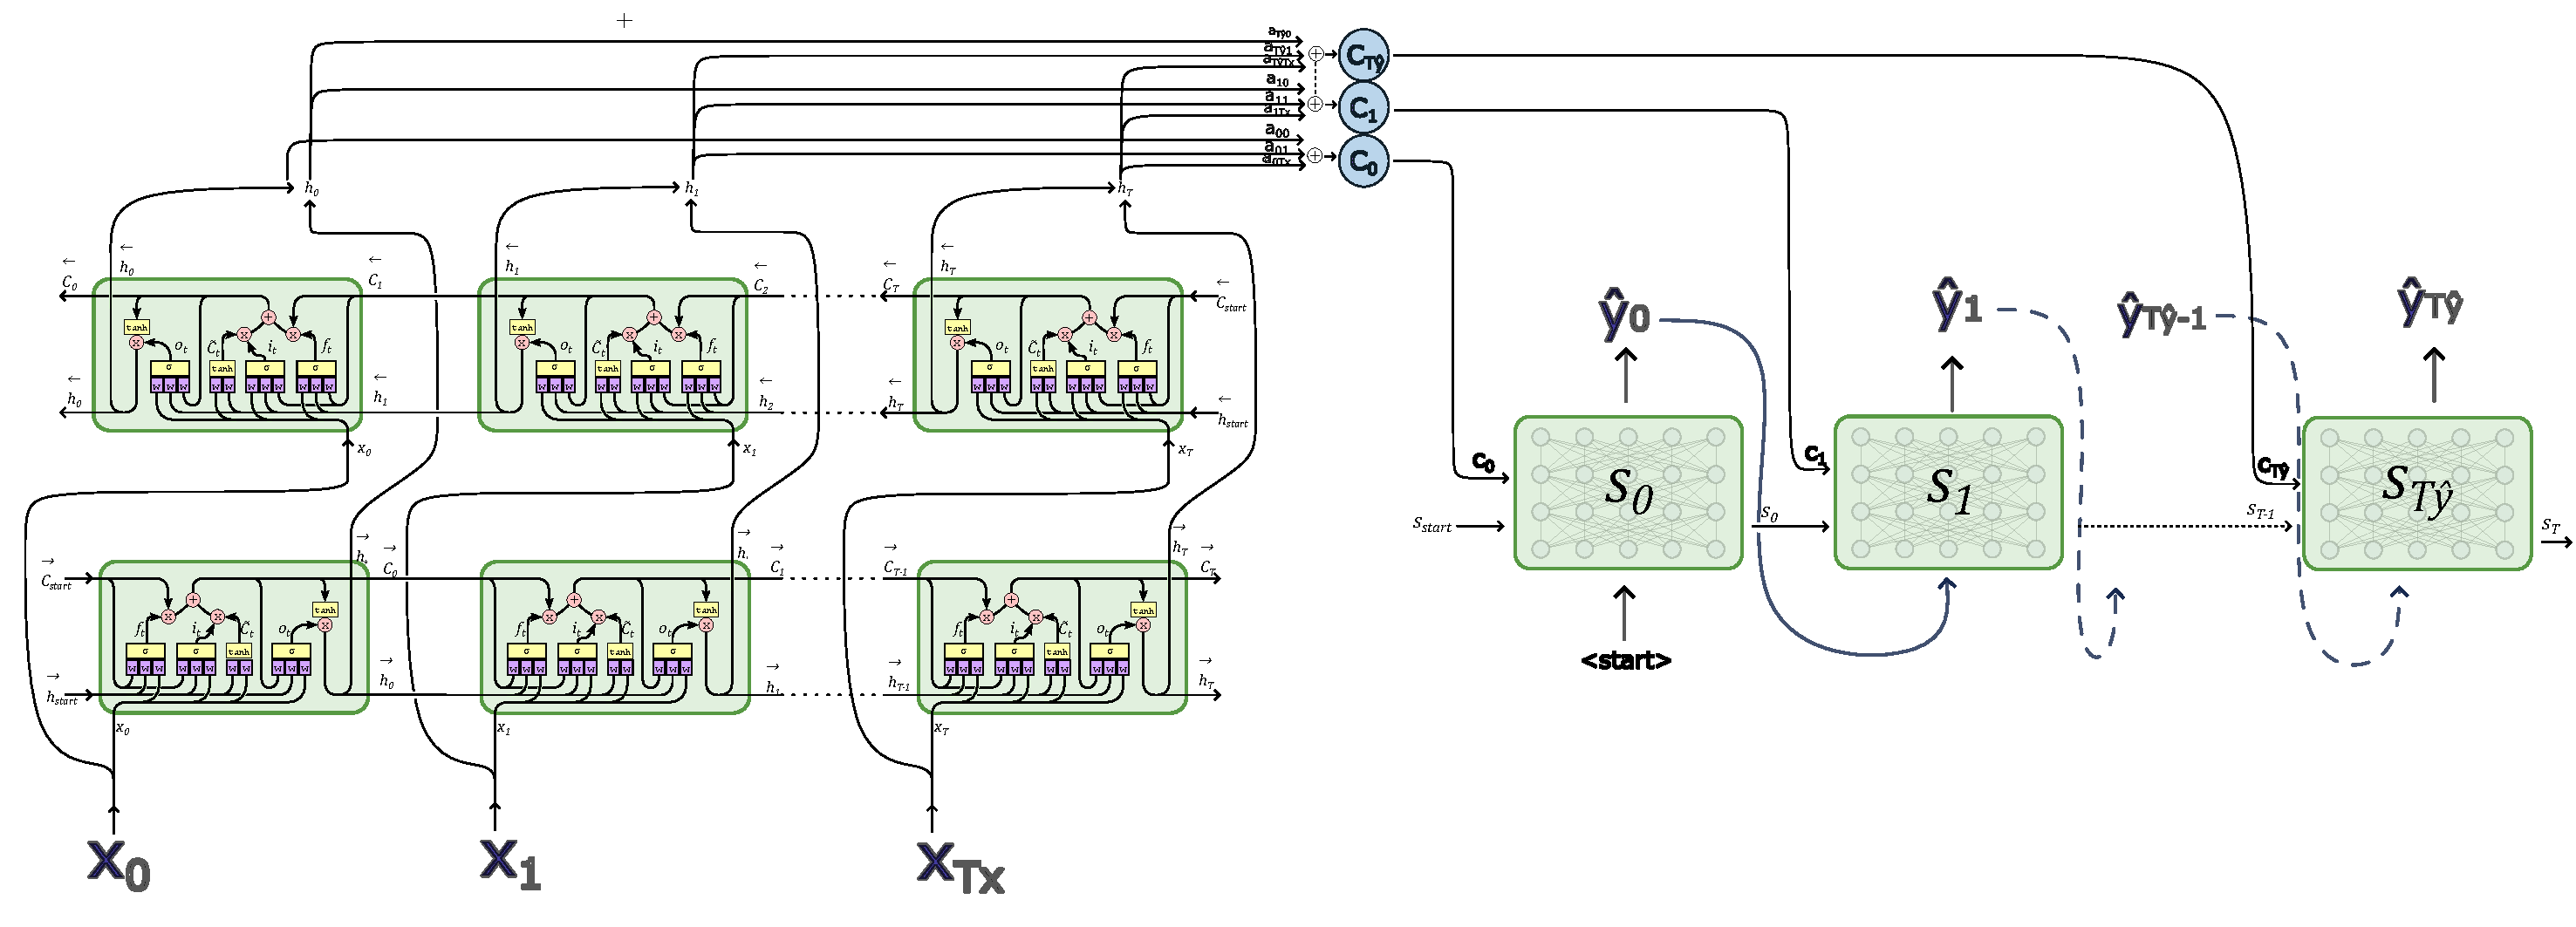
\includegraphics[width=0.95\textwidth]{images/chapter theoritical background/rnn_peaky_encoder_decoder_with_attention.pdf}
  \caption{Σχήμα στο οποίο απεικονίζεται η αρχιτεκτονική ενός επαναληπτικού νευρωνικού δικτύου τύπου κωδικοποιητή\textendash αποκωδικοποιητήχρησιμοποιώνταςμηχανισμό προσοχής. Παρατηρούμε ότι σε κάθε καρέ του αποκωδικοποιητή υπάρχει διαθέσιμο ένα ξεχωριστό διάνυσμα συμφραζόμενων (\en{context vector}). Το διάνυσμα σε κάθε καρέ σχηματίζεται ως σταθμισμένο άθροισμα των κρυφών καταστάσεων $h_t$ ανάλογα με το σε ποια σημεία της ακολουθίας εισόδου πρέπει να εστιάσει ο αποκωδικοποιητής για το συγκεκριμένο καρέ εξόδου. \textit{Παράχθηκε από το \href{https://inkscape.org/}{\en{Inkscape}}}.}
  \label{fig:rnn_peaky_encoder_decoder_with_attention}
\end{figure}

Στο σχήμα \ref{fig:rnn_peaky_encoder_decoder_with_attention} φαίνεται το ίδιο σύστημα αλλά με μηχανισμό προσοχής. Πλέον, δεν υπάρχει συμφόρηση καθώς δεν χρησιμοποιείται μόνο ένα διάνυσμα συμφραζόμενων για να κωδικοποιήσει την πληροφορία όλων των δειγμάτων της ακολουθίας εισόδου. Αντίθετα, κάθε έξοδος \textquote{ευθυγραμμίζεται} Συνεπώς, έχουμε:
\[
  s_t = f(s_{t-1}, y_{t-1}, c_t)
\]
Όπου τα διανύσματα συμφραζόμενων υπολογίζωνται ως σταθμισμένα αθροίσματα των διανυσμάτων κατάστασης, δηλαδή:
\[
  c_t = \sum_{j = 1}^{j=T_x} \alpha_{tj}\times h_j .
\]
Τα βάρη $\alpha_{tj}$ αναπαριστούν την σημασία του εκάστοτε διανύσματος κατάστασης $h_j$ στους υπολογισμούς της εξόδου την χρονική στιγμή $t$. Με άλλα λόγια, στην εφαρμογή της μετάφρασης δείχνουν σε ποιες λέξεις εισόδου πρέπει να εστιάσει σε κάθε βήμα ο αποκωδικοποιητής.\par

Σε τελική ανάλυση, για τα βάρη $\alpha_{tj}$ επιβάλουμε να ισχύει $\sum_{j = 1}^{j=T_x} \alpha_{tj} = 1$ (κανονικοποίηση) ώστε να δημιουργούν μια κατανομή πιθανότητας. Αυτό το επιτυγχάνουμε ορίζοντας τις ενέργειες $\epsilon_{tj}$ ως τιμές σημασίας που έχει το δείγμα εισόδου $X_j$ για την πρόβλεψη $\hat{y}_t$ και υπολογίζοντας τα βάρη ως εξής:
\[
  a_{tj} = \frac{\exp{\epsilon_{tj}}}{\sum_{k=1}^{T_x}exp{\epsilon_{tk}}}
.\]
\par

Μένει τώρα να περιγράψουμε το κριτίριο με το οποίο υπολογίζουμε τις τιμές ενέργειας $\epsilon_{tj}$ και συνεπώς τα βάρη $\alpha_{tj}$. Ουσιαστικά, οι τιμές ενέργειας υπολογίονται σύμφωνα με την συμφωνία που παρατηρείται μεταξύ του διανύσματος κατάστασης του αποκωδικοποιητή τη χρονική στιγμή $t$ (ονομάζεται και ερώτημα - \en{query}) και των διανυσμάτων κατάστασης του κωδικοποιητή (ονομάζονται και κλειδιά - \en{keys}). Έτσι έχουμε:
\[
  e_{tj} = \alpha(s_{t-1}, h_j)
\] Όπου εδώ $\alpha$ είναι η συνάρτηση που μετρά την συμφωνία ή ευθυγράμιση. Η πιο απλή υλοποίηση μιας τέτοιας συνάρτησης είναι με την συνάρτηση συνημιτόνου (στην περίπτωση που τα διανύσματα έχουν ίδιο μήκος). Στο έργο των \en{Bahdanau D. et al.} \cite{bahdanau2014neural_machine_translation_attention_begins} υλοποιείται η συνάρτηση ευθυγράμισης με ένα πλήρως διασυνδεδεμένο νευρωνικό δίκτυο του οποίου οι παράμετροι εκπαιδεύονται μαζί με τις υπόλοιπες παραμέτρους του μοντέλου.

\subsection{Μετασχηματιστές}
Ενώ τα αμφίδρομα νευρωνικά δίκτυα με μακροπρόθεσμη\textendash βραχυπρόθεσμη μνήμη και μηχανισμό προσοχής μετριάζουν σημαντικά τα δύο πρώτα από τα τρία προβλήματα που αναφέραμε, το τρίτο πρόβλημα παραμένει ανεπιλυτο. Για την ακρίβεια, η φύση των επαναληπτικών νευρωνικών δικτύων είναι τέτοια ώστε να απαιτείται σειριακή επεξεργασία των δειγμάτων μιας ακολουθίας, γεγονός που αυξάνει σημαντικά τους χρόνους επεξεργασίας εμποδίζωντας την κλιμάκωσή τους σε πιο σύνθετες εφαρμογές. Συνεπώς, απαιτείται μια νέα αρχιτεκτονική που θα είναι απαλλαγμένη από την σειριακή επεξεργασία ενώ θα ικανοποιεί συγχρόνως τις τέσσερεις σχεδιαστικές αρχές για την μοντελοποίηση ακολουθιών που προαναφέραμε.\par

\begin{figure}[h]
  \centering
  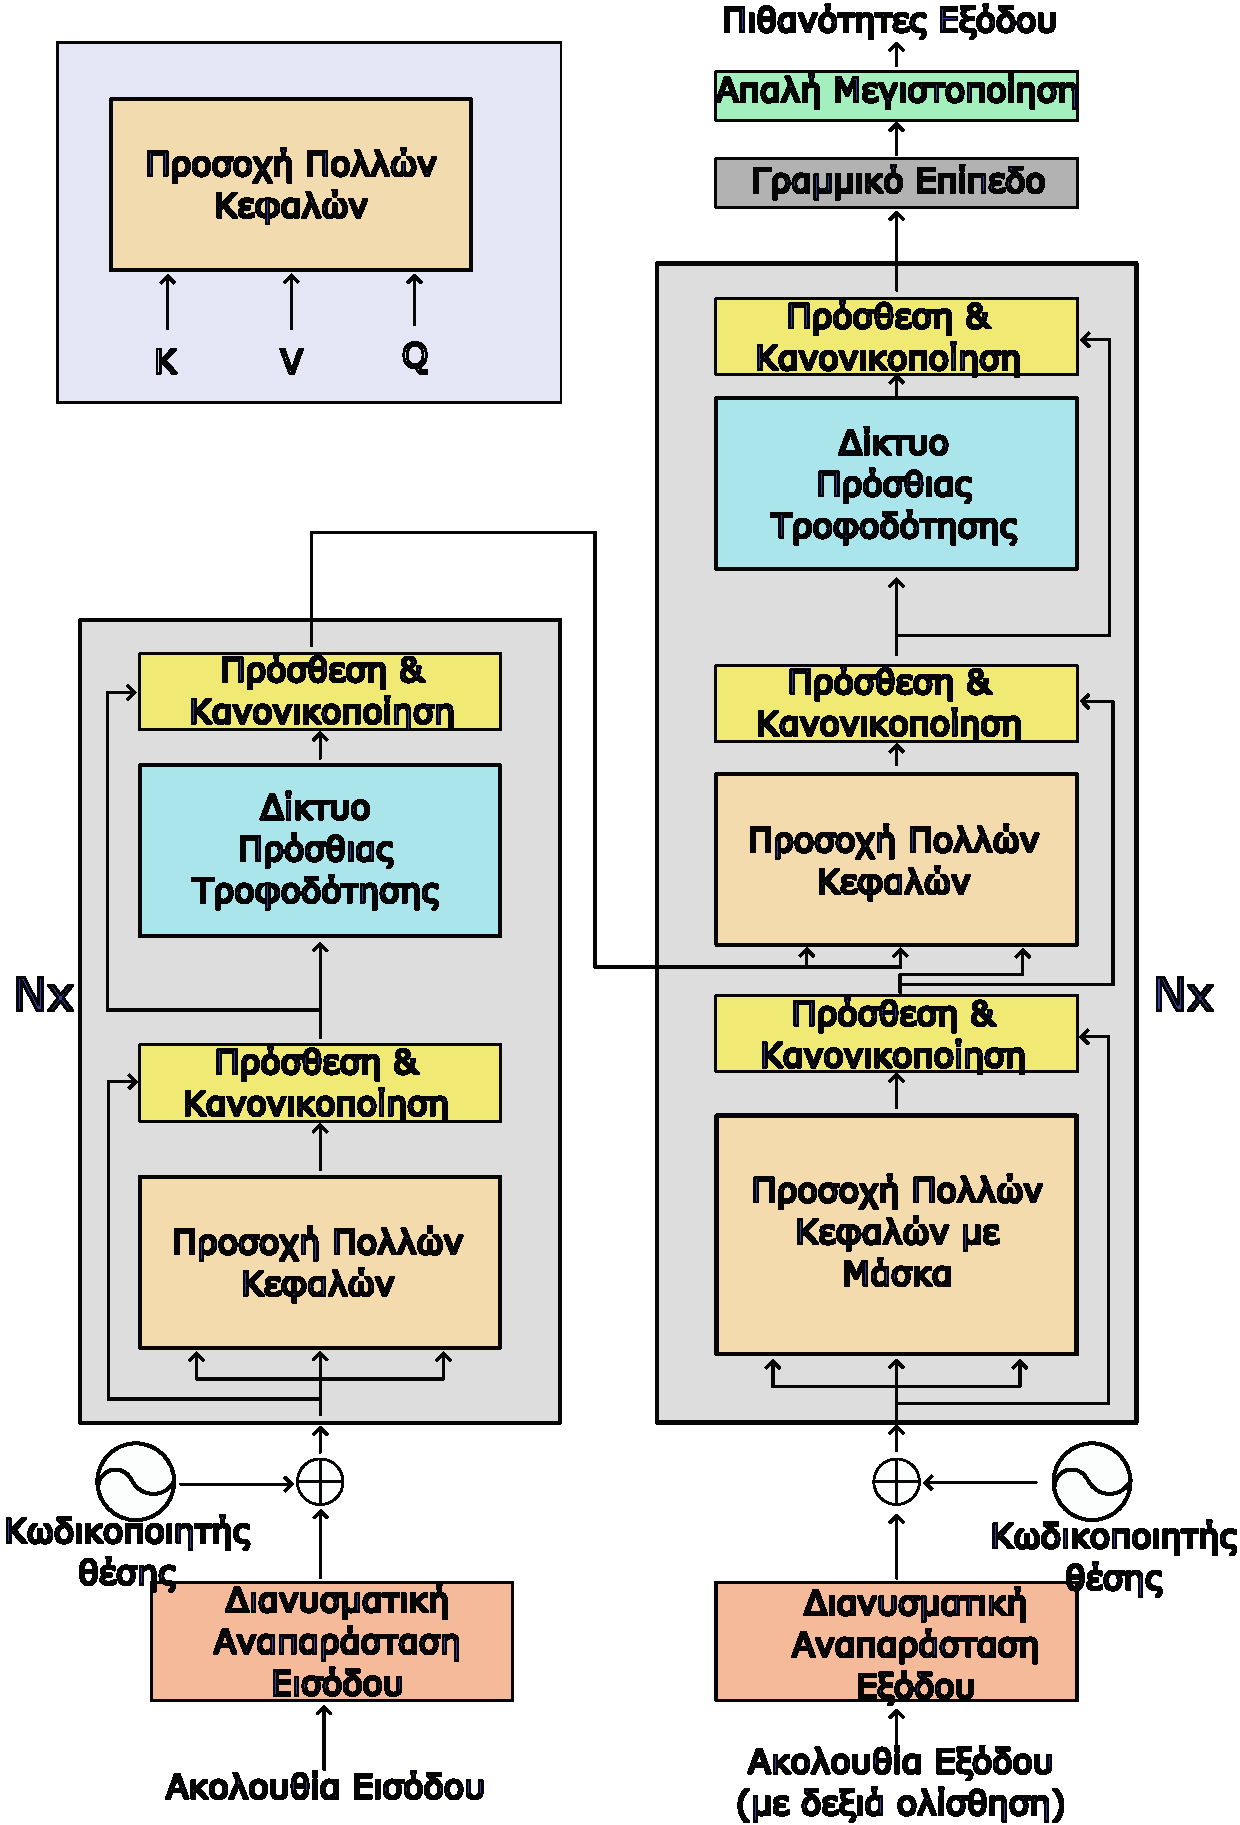
\includegraphics[width=0.7\textwidth]{images/chapter theoritical background/transformer_gr.pdf}
  \caption{Η αρχιτεκτονική ενός μετασχηματιστή\cite{transformers_attention_is_all_you_need}. \textit{Παράχθηκε από το \href{https://inkscape.org/}{\en{Inkscape}}}.}
  \label{fig:transformer}
\end{figure}

Λύση στο πρόβλημα αυτό έδωσαν οι \en{Vaswani A. et al.} με την δημοφιλή δημοσίευση υπό τον τίτλο \textquote{\en{Attention Is All You Need}}. Στο έργο τους, περιγράφουν την αρχιτεκτονική του μετασχηματιστή, όπως αυτή φαίνεται στο σχήμα \ref{fig:transformer}. Πρόκειται για μια αρχιτεκτονική νευρωνικού δικτύου υπό μορφή κωδικοποιητή\textemdash αποκωδικοποιητή που εμπεριέχει μόνο μηχανισμούς αυτο\textendash προσοχής και πλήρως διασυνδεδεμένων επιπέδων για εφαρμογές μετάφρασης ακολουθιών από λέξεις. Αυτή η νέα αρχιτεκτονική μπορεί και ικανοποιεί πλήρως όλες τις σχεδιαστικές αρχές των συστημάτων μοντελοποίησης ακολουθιών επιτρέποντας την παράλληλη επεξεργασία δειγμάτων εντός της ίδιας ακολουθίας\footnote{Αν και η νέα αρχιτεκκτονική φαίνεται αρκετά εξειδικευμένη, στην πραγματικότητα είναι γενικότερη από τα νευρωνικά δίκτυα πρόσθιας τροφοδότησης με την έννοια των λιγότερων επαγωγικών προκαταλήψεων (\en{inductive biases}).}. \par


\subsubsection{Αποκωδικοποιητής και Κωδικοποιητής}
Το δίκτυο του σχήματος \ref{fig:transformer} μπορεί να χωριστεί σε δύο μέρη: τον αποκωδικοποιητή στα αριστερά και τον κωδικοποιητή στα δεξιά. Ας ξεκινήσουμε από το κατώτερο τμήμα του αποκωδικοποιητή, δηλαδή το επίπεδο ενσωμάτωσης (\en{embedding layer}). Επειδή ως γνωστόν ένα νευρωνικό δίκτυο δεν μπορεί να διαχειριστεί συμβολοσειρές χαρακτήρων παρά μόνο διανύσματα από αριθμούς, το επίπεδο αυτό αναλαμβάνει την αντιστοίχηση κάθε λέξης $X_i$ σε μια συγκεκριμένη αναπαράσταση από $d_{features}$ χαρακτηριστικά. Η αντιστοίχηση δεν πραγματοποιείται τυχαία αλλά με τρόπο ώστε λέξεις σημασιολογικά κοντινές να έχουν μικρή απόσταση στον χώρο αναπαράστασης $\Re^{d_{features}}$. Φυσικά, το επίπεδο ενσωμάτωσης δέχεται ολόκληρη την ακολουθία μήκους $T_x$ και παράγει ένα διάνυσμα αναπαράστασης για κάθε λέξη\textemdash δείγμα παράλληλα. Έπειτα, σε κάθε διανυσματική αναπαράσταση λέξης υπερτίθεται το διάνυσμα αναπαράστασης θέσης (\en{position embedding}) (μοναδικό για κάθε θέση στην ακολουθία) έτσι ώστε να αναγνωρίζει το μοντέλο την σειρά των δειγμάτων στην ακολουθία\footnote{Επειδή τώρα τα δείγματα μιας ακολουθίας δεν επεξεργάζονται σειριακά, απαιτείται κάποια άλλη μέθοδος προκειμένου να μην παραβιάζεται η τρίτη σχεδιαστική αρχή περί διατήρησης πληροφορίας σειράς δειγμάτων.}. Τέλος, οι προκύπτουσες αναπαραστάσεις μπορούν να συνδειαστούν σε έναν πίνακα $\boldsymbol{X}$ με μέγεθος $T_x \times d_{features}$.\par

Συνεχίζοντας την περιγραφή του σχήματος \ref{fig:transformer} σύμφωνα με την ροή της πληροφορίας εισόδου δηλαδή από κάτω προς τα πάνω και από τα αριστερά προς τα δεξιά, συναντάμε το μπλόκ του αποκωδικοποιητή το οποίο δέχεται τρία αντίραφα του πίνακα $\boldsymbol{X}$. Ο αποκωδικοποιητής μπορεί να αποτελείται από $N$ επίπεδα (βλ. σχήμα \ref{fig:transformer_many_many}). Κάθε επίπεδο απαρτίζεται από δύο υπο\textendash επίπεδα: το πρώτο σχηματίζεται από τον μηχανισμό αυτο\textendash προσοχής πολλαπλών κεφαλών (\en{multi\textendash head attention}) και το δεύτερο από ένα νευρωνικό δίκτυο πρόσθιας τροφοδότησης με δύο πλήρως διασυνδεδεμένα επίπεδα που δρα με τον ίδιο τρόπο σε κάθε διάνυσμα λέξης (\en{position\textendash wise}). Γύρω από το καθένα υπο\textendash επίπεδο υπάρχει μια υπολλειματική σύνδεση (\en{residual connection}), ακολουθούμενη από κανονικοποίηση επιπέδου (\en{layer normalization})\footnote{Βλέπε παράρτημα \ref{chap:definitions}}. Με άλλα λόγια, αν συμβολίσουμε την έξοδο κάθε υπο\textendash επιπέδου ως $Sublayer(\boldsymbol{X})$ τότε η έξοδος μετά από κάθε υποεπιπέδου μαζί με την υπολειματική σύνδεση (\en{residual connection}) και την κανονικοποίηση επιπέδου (\en{layer normalization}) είναι $LayerNorm(\boldsymbol{X} + Sublayer(\boldsymbol{X}))$. Τελικά, ο αποκωδικοποιητής παράγει (παράλληλα) σαν έξοδο μια ακολουθία $\boldsymbol{Z} = [Z_1, Z_2, \dots, Z_{T_x}]$ στην οποία κάθε δείγμα περιέχει πλούσια πληροφορία για τα συμφραζόμενά του.\par

\begin{figure}[p]
  \centering
  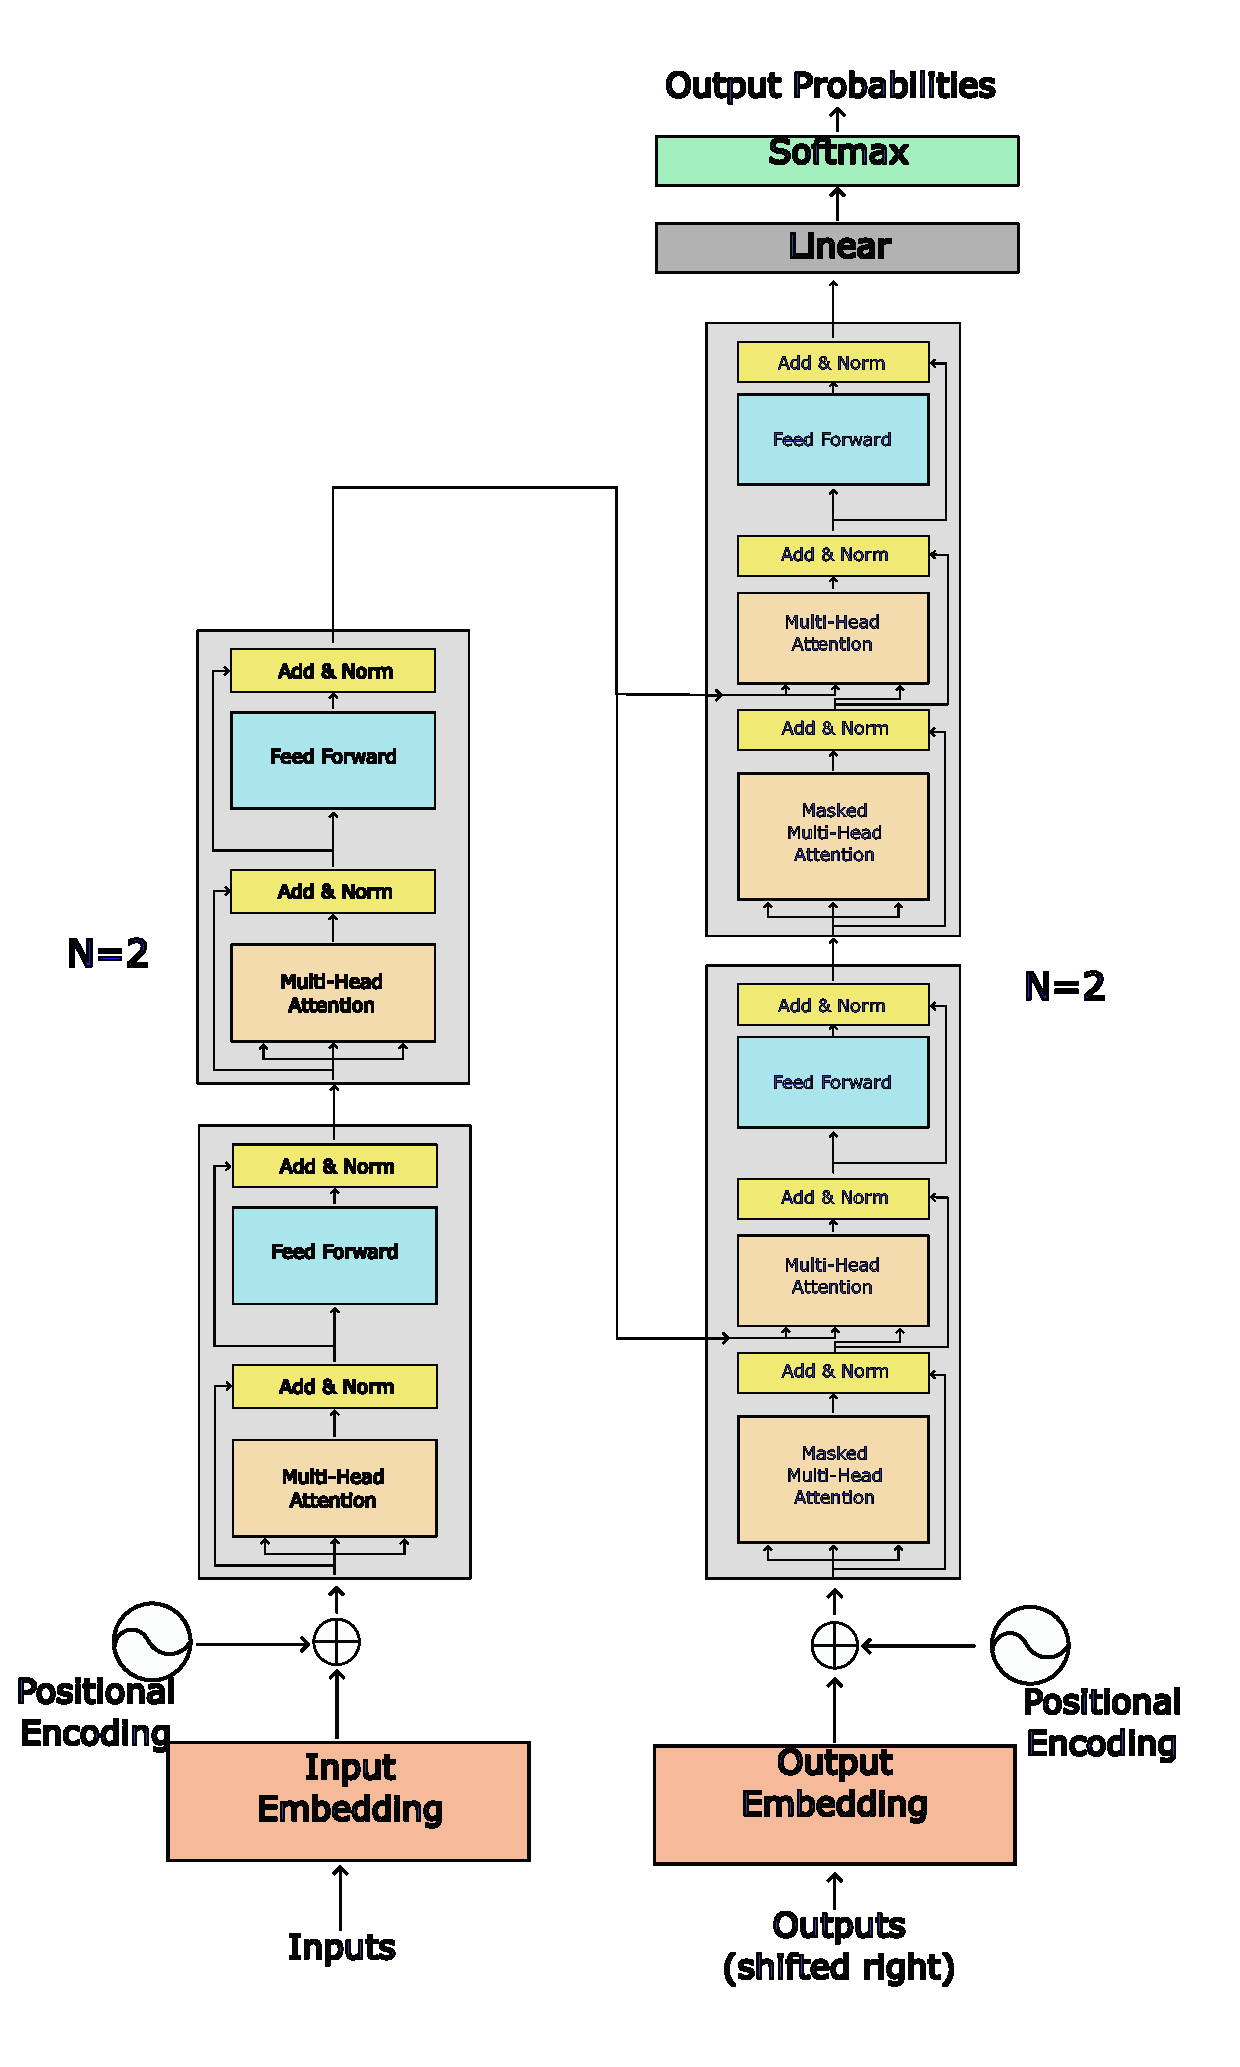
\includegraphics[width=0.8\textwidth]{images/chapter theoritical background/transformer_many_to_many.pdf}
  \caption{Η αρχιτεκτονική ενός μετασχηματιστή \cite{transformers_attention_is_all_you_need} όταν αυτός αποτελείται από πολλά μπλόκ κωδικοποιητών και αποκωδικοποιητών (στο σχήμα, δύο από το κάθε είδος μπλόκ). \textit{Παράχθηκε από το \href{https://inkscape.org/}{\en{Inkscape}}}.}
  \label{fig:transformer_many_many}
\end{figure}

Ο αποκωδικοποιητής σε γενικές γραμμές είναι ένα μοντέλο αυτοπαλινδρόμησης (\en{auto\textendash regressive model}) που δέχεται την ακολουθία $\boldsymbol{Z} = [Z_1, Z_2, \dots, Z_{T_x}]$ από τον κωδικοποιητή και τελικά παράγει σηρειακά την ακολουθία $\boldsymbol{\hat{Y}} = [\hat{Y}_1, \hat{Y}_2, \dots, \hat{Y}_{T_y}]$. Η αυτοπαλινδρόμηση έγκειται στο γεγονός ότι σε κάθε βήμα $t$, για να εξάγει το μοντέλο το διάνυσμα $\hat{Y}_t$ λαμβάνει υπόψη τις εξόδους που έχει παράξει τις προηγούμενες χρόνικές στιγμές, ολισθημένες κατά 1 θέση δεξιά, δηλαδή τα $[\mathbin{<}SOS\mathbin{>}, \hat{Y}_1, \hat{Y}_2, \dots, \hat{Y}_{t-1}]$\footnote{Η λεξικογραφική μονάδα \textquote{\en{<SOS>}} χρησιμοποιείται για να σηματοδοτήσει στον αποκωδικοποιητή την αρχή της φράσης εξόδου.}. Σε αντίθεση με τα μοντέλα επαναληπτικών νευρωνικών δικτύων με αυτο\textendash παλινδρόμηση όπου η εκπαίευση καθυστερεί, στους μετασχηματιστές δεν απαιτείται η παραγωγή ολόκληρης της ακολουθίας εξόδου για την εφαρμογή του αλογορίθμου οπισθοδιάδοσης σφάλματος. Δηλαδή, ο αλγόριθμος μάθησης εφαρμόζεται με κάθε δείγμα εξόδου.\par

Κοιτώντας το σχήμα \ref{fig:transformer} και αναλύοντάς το από κάτω προς τα πάνω παρατηρούμε ότι και ο αποκωδικοποιητής τροφοδοτείται με λέξεις σε διανυσματική αναπαράσταση μέσω του επιπέδου ενσωμάτωσης (\en{embedding layer}) και του κωδικοποιητή θέσης (\en{positional embedding}). Βέβαια, σε αντίθεση με τον κωδικοποιητή, η ακολουθία που δέχεται σαν είσοδο ο αποκωδικοποιητής απαρτίζεται από τις προηγούμενες λέξεις\textemdashστόχους (δηλαδή τις$[\mathbin{<}SOS\mathbin{>}, \hat{Y}_1, \hat{Y}_2, \dots, \hat{Y}_{t-1}]$).\par

Συνεχίζοντας την ανάλυση του σχήματος \ref{fig:transformer}, ο αποκοδικοποιητής αποτελείται από $N$ πανομοιότηπα επίπεδα (βλ. σχήμα \ref{fig:transformer_many_many}) και μπορεί να διαιρεθεί σε τρία υποεπίπεδα. Το πρώτο υπο\textendash επίπεδο είναι αυτό του μηχανισμού αυτο\textendash προσοχής πολλών κεφαλών με μάσκα (\en{masked multi\textendash head attention}). Γύρω από αυτό, όπως και από όλα τα υπο\textendash επίπεδα, υπάρχει μια υπολειματική σύνδεση που καταλήγει σε ένα επίπεδο κανονικοποίησης. Τα επόμενα δύο υπο\textendash επιπεδα είναι τα ίδια με αυτά που περιγράψαμε στην περίπτωση του κωδικοποιητή. Να σημειώσουμε ότι στο μεσαίο υπο\textendash επίπεδο, η είσοδος σχηματίζεται από την ακολουθία διανυσματικών αναπαραστάσεων των προηγηθέντων λέξεων εξόδου που παράγεται από το πρώτο υπο\textendash επίπεδο του αποκωδικοποιητή (τον πίνακα αυτό τον ονομάζουμε Ερώτημα - \en{Query} και ισχύει $Q \in \Re^{d_{features} \times {t}}$\footnote{Θεωρούμε $t=1$ τη στιγμή παραγωγής της πρώτης εξόδου $\hat{Y}_1$.}) και την έξοδο του κωδικοποιητή, αντεγραμμένη δύο φορές (σχηματίζοντας δύο πίνακες, τους Κλειδί - \en{Key} και Τιμή - \en{Value}). Τέλος, το κάθε επίπεδο αποκωδικοποιητή παράγει μια έξοδο μεγέθους $t \times d_{features}$ η οποία είτε δίνεται στο επόμενο επίπεδο κωδικοποιητή είτε, αν δεν υπάρχει κάποιο επόμενο επίπεδο, μετασχηματίζεται μέσω ένος γραμμικού, πλήρως διασυνδεδεμένου επιπέδου το οποίο έχει σαν έξοδο ένα διάνυσμα $Z_{out} \in \Re^{vocabulary size}$. Το τελευταίο, αφού περάσει από την συνάρτηση απαλής μεγιστοποίησης (\en{softmax}) αποτελεί την έξοδο που είναι πρακτικά μια κατανομή διακριτής πιθανότητας πάνω σε όλο το λεξιλόγιο. Η λέξη με την μέγιστη πιθανότητα είναι και η πρόβλεψη $\hat{Y}_t$\footnote{Εκτός αν χρησιμοποιείται ακτινική αναζήτηση \en{beam search}.}.

\subsubsection{Υπο\textendash επίπεδο Νευρωνικού Δικτύου Πρόσθιας Τροφοδότησης}
Πρόκειται για το τελευταίο υπο\textendashεπίπεδο τόσο του μπλόκ αποκωδικοποιητή όσο και του μπλόκ κωδικοποιητή και σχηματίζεται από δύο πλήρως διασυνδεδεμένα επίπεδα από τεχνητούς νευρώνες (δεν προσμετράμε το επίπεδο εισόδου). Οι νευρώνες του πρώτου επιπέδου χρησιμοποιούν την συνάρτηση ενεργοποίησης \textquote{\en{ReLU}} ενώ οι νευρώνες του δεύτερου την ταυτοτική συνάρτηση. Έτσι, έχουμε:
\[
  FFN(X) = max(0, X \times W^{[1]} + b^{[1]})\times W^{[2]} + b^{[2]}
\]όπου $W^{[1]}, b^{[1]}, W^{[2]}, b^{[2]}$ παράμετροι που μαθαίνονται κατά την εκπαίδευση.\par

Όπως είπαμε, η συνάρτηση του νευρωνικού δικτύου εφαρμόζεται με τα ίδια βάρη σε κάθε δείγμα της ακολουθίας ξεχωριστά. Με άλλα λόγια, αν σαν είσοδο δίνεται ο πίνακας $\boldsymbol{X}$ με μέγεθος $T_x \times d_{features}$ τότε η ίδια συνάρτηση θα εφαρμοστεί $T_x$ φορές\footnote{Το ίδιο δίκτυο θα μπορούσαμε να διατυπώσουμε διαφορετικά ότι αποτελείται από δύο συνελικτικά επίπεδα με μοναδιαίο πυρήνα (\en{point\textendash wise convolutional layers}).}. \par

\subsubsection{Μηχανισμός Προσοχής Πολλών Κεφαλών}
Κατά αναλογία με τον μηχανισμό πρόσοχής ο οποίος δέχεται δύο διαφορετικές ακολουθίες, ο μηχανισμός αυτο\textendash προσοχής συσχετίζει τα δείγματα μιας μεμονομένης ακολουθίας μεταξύ τους προκειμένου να υπολογίσει μια άλλη αναπαράσταση αυτής της ακολουθίας. 
Από το σχήμα \ref{fig:transformer} έχουμε παρατηρίσει ότι το υπο\textendash επίπεδο που υλοποιεί τον μηχανισμό αυτοπροσοχής δέχεται τρείς εισόδους. Αυτές συμβολίζονται - όπως έχουμε αναφέρει - με τα γράμματα \en{Q} (Ερώτημα - \en{Query}), \en{K} (Κλειδί - \en{Key}) και \en{V} (Τιμή - \en{Value}). Οι ονομασίες αυτές δεν είναι τυχαίες. Διαισθητικά, το Ερώτημα χρησιμοποιείται για την αναζήτηση των κατάλληλων Κλειδιών στα οποία θα δοθεί προσοχή με παρόμοιο τρόπο με τον οποίο μια μηχανή αναζήτησης διπλωματικών εργασιών χρησιμοποιεί τους όρους αναζήτησης και εξετάζει την ομοιότητά τους με τις λέξεις κλειδιά της κάθε εργασίας. Η τιμή, στο παράδειγμά μας, θα μπορούσε να είναι το περιεχόμενο της κάθε διατριβής. \par

\begin{figure}[h]
  \centering
  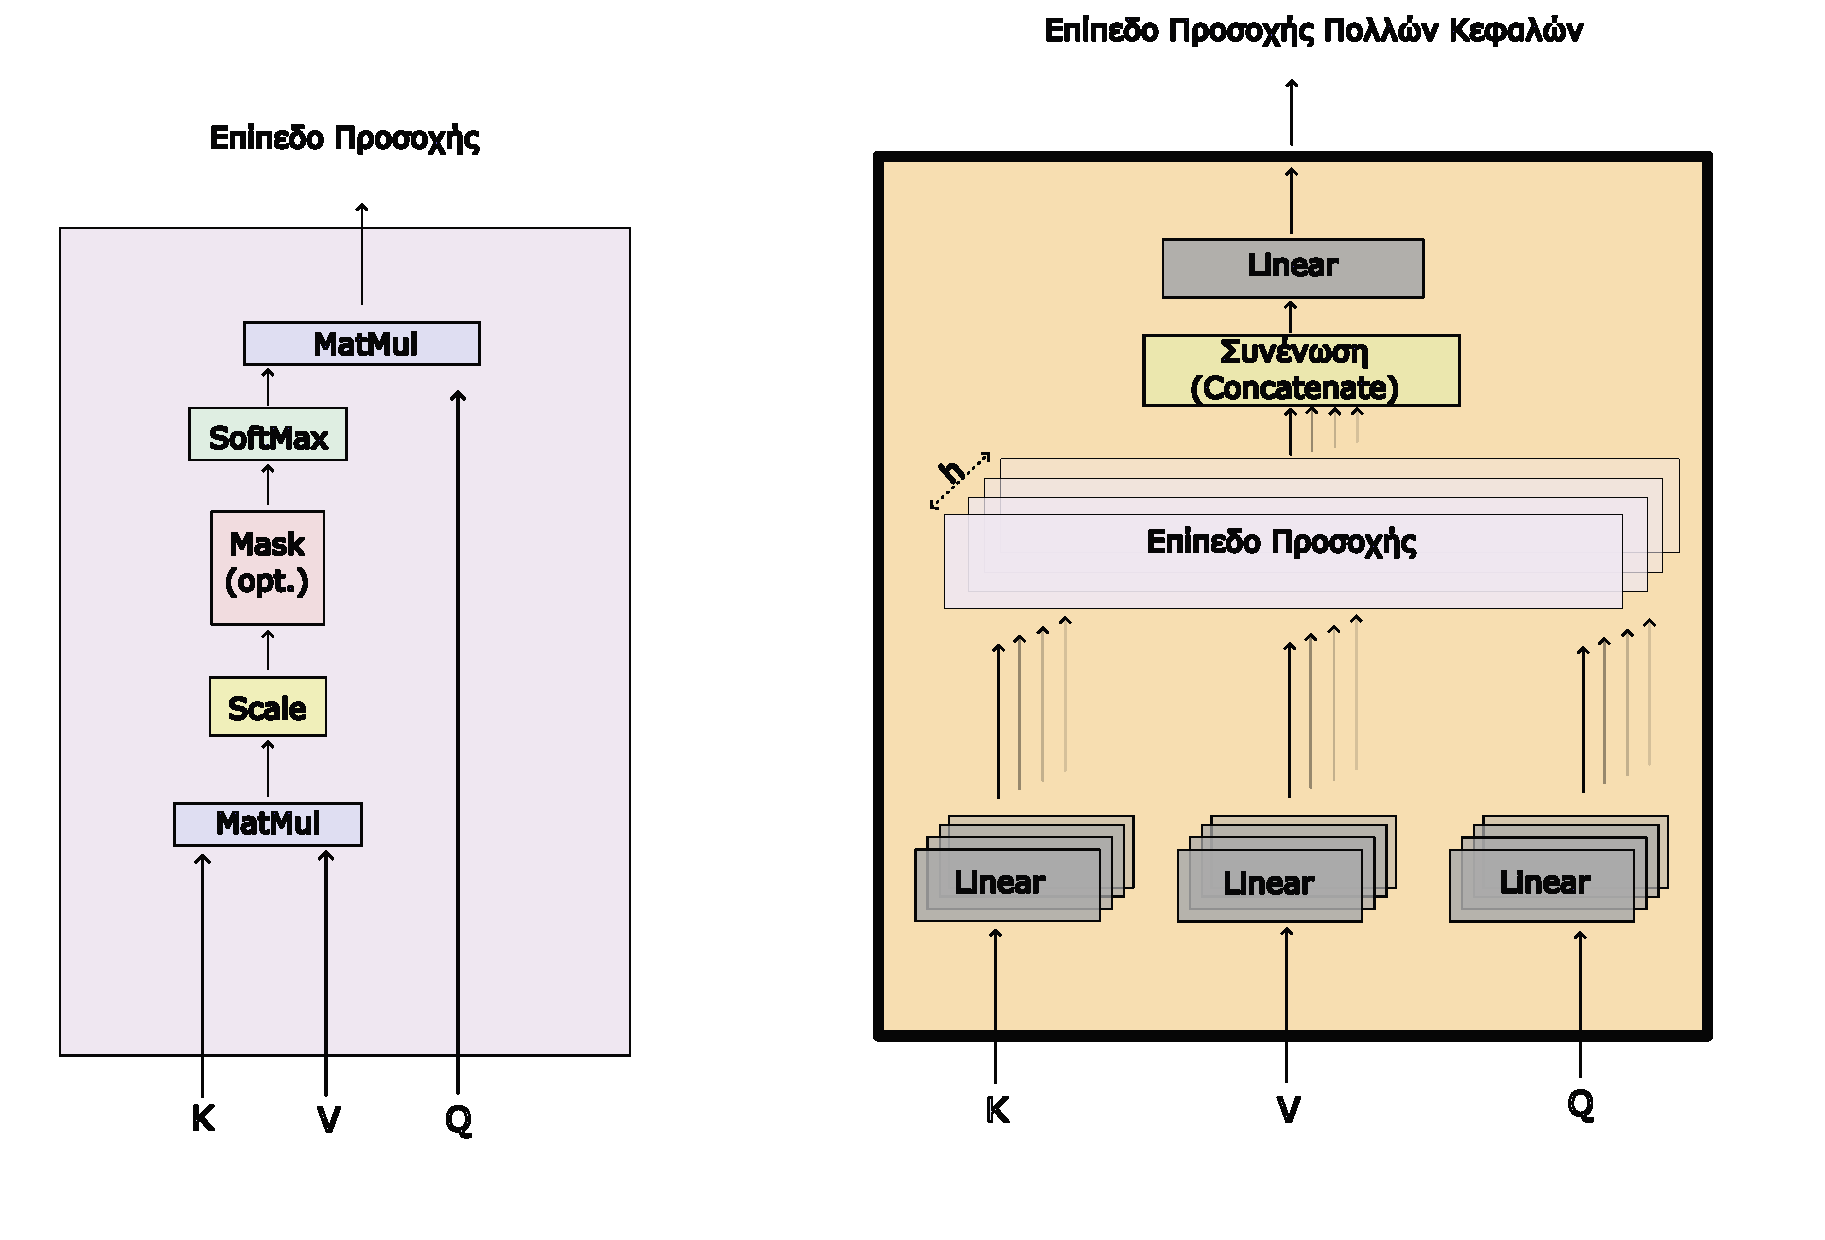
\includegraphics[width=0.8\textwidth]{images/chapter theoritical background/transformer_attention_gr.pdf}
  \caption{Το μπλοκ προσοχής πολλών κεφαλών (αριστερά) και το μπλοκ προσοχής με κλιμακωτό εσωτερικό γινόμενο (αριστερά). \textit{Παράχθηκε από το \href{https://inkscape.org/}{\en{Inkscape}}}.}
  \label{fig:transformer_multi_head}
\end{figure}

Για την λεπτομερή εξέταση της υλοποίησης του μηχανισμού προσοχής πολλών κεφαλών παρουσιάζεται το σχήμα \ref{fig:transformer_multi_head}. Σε αυτό διακρίνεται η πολυεπίπεδη φύση του υπο\textendash επιπέδου. Πιο αναλυτικά, σε κάθε επίπεδο\textemdash κεφαλή $h_i, i \in [1,n_h]$ τα διανύσματα $Q, K, V$ προβάλλονται μέσω γραμμικών επιπέδων (πινάκων παραμέτρων $W_i^Q, W_i^K, W_i^V$ αντίστοιχα) στα $Q_i, K_i, V_i$. Έπειτα, πραγματοποιείται η \textquote{προσοχή με κλιμακωτό εσωτερικό γινόμενο} (\en{Scaled Dot-Product Attention}). Το αποτέλεσμα των επιπέδων ενώνεται σε ένα πίνακα ο οποίος τελικά διέρχεται απο ένα γραμμικό επίπεδο (με βάρη που συμβολίονται ως $W^O$). \par

\begin{figure}[p]
  \centering
  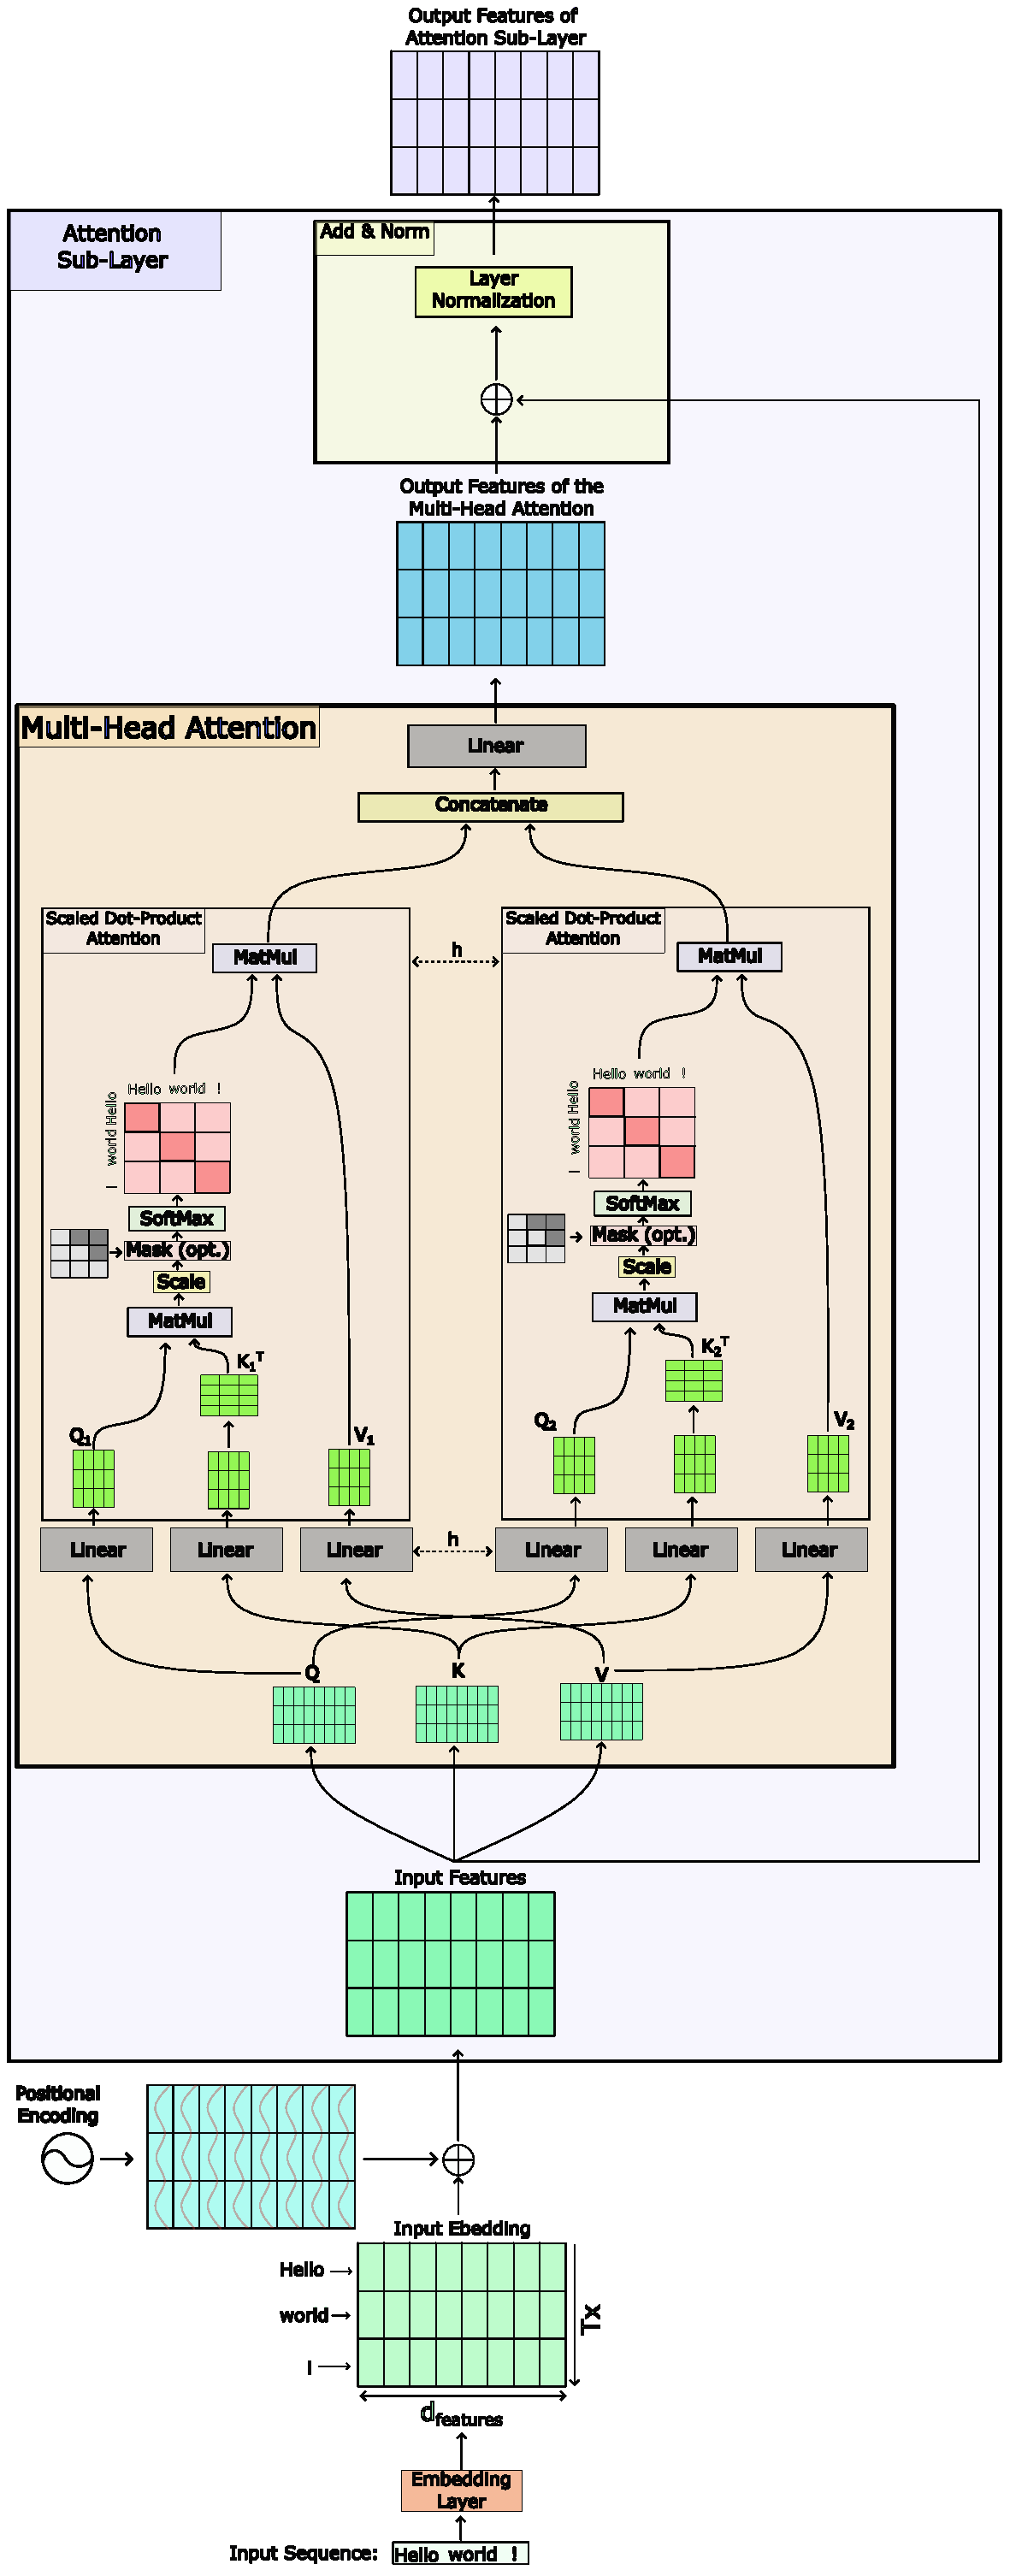
\includegraphics[width=0.55\textwidth]{images/chapter theoritical background/transformer_flow.pdf}
  \caption{Παράδειγμα της ροής πληροφορίας σε ένα υπο\textendash επίπεδο προσοχής. Στο συγκεκριμένο παράδειγμα χρησιμοποιούνται δύο κεφαλές με $d_{features} = 8$ και $d_k=d_v=4$. Αν και το παράδειγμα εστιάζει περισσότερο σε ενα μπλοκ κωδικοποιητή, οι διαφορές για την πρερίπτωση του κωδικοποιητή είναι ελάχιστες (η ακολουθία εισόδου θα αποτελούνταν από τις λέξεις που είχαν παραχθεί μέχρι την εκάστοτε χρονική στιγμή, ολισθημένες κατά μία θέση. Πριν παραχθεί η πρώτη λέξη, τροφοδοτείται στον αποκωδικοποιητή το σύμβολο \textquote{\en{SOS}} που σηματοδωτεί την αρχή της ακολουθίας). \textit{Παράχθηκε από το \href{https://inkscape.org/}{\en{Inkscape}}}.}
  \label{fig:transformer_flow}
\end{figure}

Συνολικά, χρησιμοποιώντας μαθηματική περιγραφή, το υπο\textendash επίπεδο προσοχής δέχεται τρείς πίνακες:

\begin{equation}
  Q \in \Re^{T \times d_{features}},K \in \Re^{T \times d_{features}}, V \in \Re^{T \times d_{features}}
\end{equation}
\begin{equation}
  \text{όπου } T = \begin{cases} 
    T_x & \text{αν } Q | K | V \text{προέρχονται από κωδικοποιητή}\\
    t & \text{αν } Q | K | V \text{προέρχονται από αποκωδικοποιητή}
  \end{cases} 
\end{equation}
 

  
  Έπειτα, για τα τρία διανύσματα αυτά, υπολογίζονται τόσες προβολές όσος και ο αριθμός κεφαλών $n_h$. Δηλαδή για την $i$ καφαλή έχουμε έχουμε:
  \begin{equation}
    Q_i = Q\times W_i^Q, K_i = K \times W_i^K, V_i = V \times W_i^K,
  \end{equation}
  \begin{equation}
    \text{ όπου } W_i^Q \in \Re^{d_{features} \times d_k}, W_i^K \in \Re^{d_{features} \times d_k}, W_i^V \in \Re^{d_{features} \times d_v}
  \end{equation}

  Παρατηρούμε ότι με την προβολή, το μήκος του αριθμού χαρακτηριστικών για κάθε δείγμα της ακολουθίας μετατρέπεται από $d_{features}$ σε $d_k$ ή $d_v$. Συνήθως, επιλέγεται $d_k = d_v = d_{features}/h$ προκειμένου το υπολογιστικό κόστος να μην πολλαπλασιάζεται καθώς αυξάνεται ο αριθμός των κεφαλών.
  Εν συνεχεία, για την κάθε κεφαλή πραγματοποιούμε τις ενέργειες του δεξιού σχήματος της εικόνας \ref{fig:transformer_multi_head}. Με μαθηματικούς όρους, είναι:
  \[
    Attention(Q_i, K_i, V_i) = Softmax(\frac{Q_i\times K_i^T}{\sqrt[2]{d_k}} \odot M) \times V_i
    \]
    όπου για ένα πίνακα 
    \[ 
      \boldsymbol{X} = \underset{(\alpha \times \beta)}{\begin{bmatrix}
        & X_1 &  \\
        & X_2 &  \\
        & \vdots & \\
        & X_{\alpha} &  
      \end{bmatrix}}
      \] 
      ορίζουμε
    \[
      Softmax(\boldsymbol{X}) =
      \begin{bmatrix}
        & softmax(X_1) &  \\
        & softmax(X_2) &  \\
        & \vdots & \\
        & softmax(X_{\alpha}) &  
      \end{bmatrix}
        \]
        και όπου $M \in \Re^{T \times T}$.

  Ορίζουμε τον προαιρετικό πίνακα μάσκας $M$ με ίδιες διαστάσεις με τον $Q_i\times K_i^T$. Οι δύο πίνακες πολλαπλασιάζονται σημειακά ώστε στην περίπτωση της διαδικασίας αποκωδικοποίησης, κατά την εκπαίδευση όπου είναι από πριν γνωστή η επιθυμητή ακολουθία εξόδου $\boldsymbol{Y}$, το μοντέλο να μην βλέπει τα μελλοντικά δείγματα στόχους. Ο πίνακας $M$ είναι κάτω τριγωνικός με τα μη\textendash μηδενικά στοιχεία ίσα με πλήν άπειρο.\par
  
  Το αποτέλετσμα της συνάρτησης \en{Softmax} είναι ένας πίνακας με διαστάσεις $T \times T$ ο οποίος δείχνει τη συσχέτιση (βαθμός ομοιότητας) μεταξύ των δειγμάτων στις ακολουθίες $K_i$ και $Q_i$. Προφανώς, κάθε γραμμή είναι κανονικοποιημένη ώστε να αποτελεί μια κατανομή πιθανότητας. Θα τον ονομάζουμε και χάρτη προσοχής (\en{attention map}). Δηλαδή:
  \[
    AttentionMap(Q_i, K_i) = softmax(\frac{Q_i\times K_i^T}{\sqrt[2]{d_k}} \times M).
    \]
  
  Αφού γίνει και ο πολλαπλασιασμός με τον πίνακα των τιμών, ενώνουμε τα αποτελέσματα κάθε κεφαλής σε ένα διάνυσμα και τα περνάμε από ένα γραμμικό επίπεδο ώστε να λάβουμε ένα πίνακα με δείγματα μήκους $d_{features}$, δηλαδή: 
  \begin{equation}
    MultiHead(Q, K, V) = [ head_1^{\frown}head_2^{frown}\dots head_{n_h} ] \times W^O
  \end{equation}
  όπου 
  \[
    head_i = Attention(Q_i, K_i, V_i) \text{ και } W^O \in \Re^{n_h d_v \times d_{features}}.
  \]



 

\section{Χάρτες Αυτο-οργάνωσης}
\label{sec:_SOM}
Η τελευταία έννοια που αναπτύσουμε στο κεφάλαιο αυτό είναι αυτή του \textquote{χάρτη αυτο\textendash οργάνωσης} (\en{self\textendash organizing map - SOM}) \cite{kohonen1982self, kohonen1990self}. Αφορά την τεχνική μη\textendash επιβλεπόμενης μάθησης η οποία παράγει μια χαμηλής διαστατικότητας απεικόνιση (συνήθως δισδιάστατη) ενός συνόλου δεδομένων υψηλής διαστατικότητας, διατηρώντας την τοπολογική δομή τους. Για να εξηγήσουμε περεταίρω την τεχνική αυτή που θα χρησιμοποιήσουμε στην συνέχεια, θα περιγράψουμε πρώτα τι είναι η ανταγωνιστική μάθηση. Έπειτα, θα αναφερθούμε στην αρχιτεκτονική ενός χάρτη που ακολουθεί το μοντέλο \en{Kohonen}. Στη συνέχεια, θα κάνουμε μια νύξη στην τοπογραφική οργάνωση οργάνωση του εγκεφαλικού φλοιού και πως αυτό το χαρακτηριστικό ενέμπνευσε την παρούσα τεχνολογία. Τέλος, θα παρουσιάσουμε τον αλγόριθμο σχηματισμού ενός χάρτη αυτο\textendash οργάνωσης.

\subsubsection{Ανταγωνιστική Μάθηση}

Οι χάρτες αυτο\textendash οργάνωσης αποτελούνται από μια ειδική κατηγορία τεχνητών νευρωνικών δικτύων που βασίζονται σε ένα είδος μη\textendash επιβλεπόμενης μάθησης, την ανταγωνιστική μάθηση (\en{competitive learning})\cite{haykin2009neural}. Πιο αναλυτικά, στο τεχνητό νευρωνικό δίκτυο, οι νευρώνες ανταγονίζονται μεταξύ τους για το δικαίομα ενεργοποίησης (\en{excitation}), με αποτέλεσμα μόνο ένας νευρώνας εξόδου (ή ένας νευρώνας ανα ομάδα) να είναι ενεργός κάθε στιγμή. Το κριτήριο ενεργοποίησης ενός νευρώνα είναι ο βαθμός με τον οποίο ο νευρώνας μπορεί να εξηγήσει το εκάστοτε διάνυσμα εισόδου $x_i$ (τραβηγμένο τυχαία από ένα σύνολο δεδομένων $S_n$). Ο νευρώνας που ενεργοποιείται στην είσοδο $x_i, i \in [1,n]$ αποκαλείται νευρώνας νικιτής και απολαμβάνει την μεγαλύτερη τροποποίηση ώστε να αναπαριστά πιστώτερα την είσοδο $x_i$. Στην ειδική περίπτωση που μόνο ο νευρώνας νικητής προσαρμόζεται στο διάνυσμα εισόδου τότε λέμε ότι αυτός απολαμβάνει το καθεστώς του \textquote{ο νικιτής τα παίρνει όλα} (\en{winner takes it all})\footnote{Στο μοντέλο που θα εξετάσουμε, δεν ισχύει αυτό το καθεστός αφού ο νικιτής νευρώνας δεν είναι ο μόνος που τροποποιείται ανάλογα με την είσοδο.}. \par

\subsection{Αρχιτεκτονική Χάρτη Αυτο\textendash οργάνωσης}

Στο σχήμα \ref{fig:SOM} παρουσιάζεται η αρχιτεκτονική ενός χάρτη αυτο\textendash οργάνωσης που ακολουθεί το μοντέλο του \en{Kohonen}\footnote{Ένα άλλο μοντέλο είναι το λιγότερο δημοφιλές μοντέλο του \en{Willshaw - von der Malsburg} το οποίο όμως ξεφεύγει από τα πλαίσια της παρούσας διπλωματικής εργασίας.}. Παρατηρούμε ότι οι τεχνητοί νευρώνες οργανώνονται σε ένα δισδιάστατο πλέγμα (\en{lattice}) από κόμβους, μεγέθους $d_x \times d_y$. Ο κάθε νευρώνας $w_j, j \in [1, d_x \times d_y]$, αποτελείται από τόσα βάρη όση και η διάσταση των διανυσμάτων εισόδου ($m$), δηλαδή $w_j = [w_{j1}, w_{j2}, \dots, w_{jm}]$. Θα συμβολίζουμε το σύνολο όλων των νευρώνων του πλέγματος με το σύμβολο $\mathcal{A}$. Χάρη στην ανταγωνιστική μάθηση που εξηγήσαμε παραπάνω, οι νευρώνες συντονίζονται (\en{tuned}) επιλεκτικά σε διάφορα πρότυπα εισόδου τροποποιώντας κατάλληλα τα βάρη τους ώστε να τα αναπαριστούν καλύτερα. Ο συντονισμός γίνεται με τέτοιο τρόπο ώστε οι νευρώνες σταδιακά να διατάσσονται πάνω στο πλέγμα σε θέσεις ανάλογες με το πρότυπο που αναπαριστούν, σχηματίζοντας έτσι έναν λογικό χάρτη από συστάδες (\en{clusters}). Με άλλα λόγια, \textquote{ένας αυτο\textendash οργανούμενος χάρτης χαρακτηρίζεται από το σχηματισμό ενός τοπογραφικού χάρτη αποτελούμενου από τα πρότυπα εισόδου, στον οποίο οι χωρικές θέσεις (οι συντεταγμένες) των νευρώνων στο πλέγμα είναι ενδεικτικές των εσωτερικών στατιστικών χαρακτηριστικών που περιέχονται στα πρότυπα εισόδου}\cite{haykin2009neural}. \par

\begin{figure}[h]
  \centering
  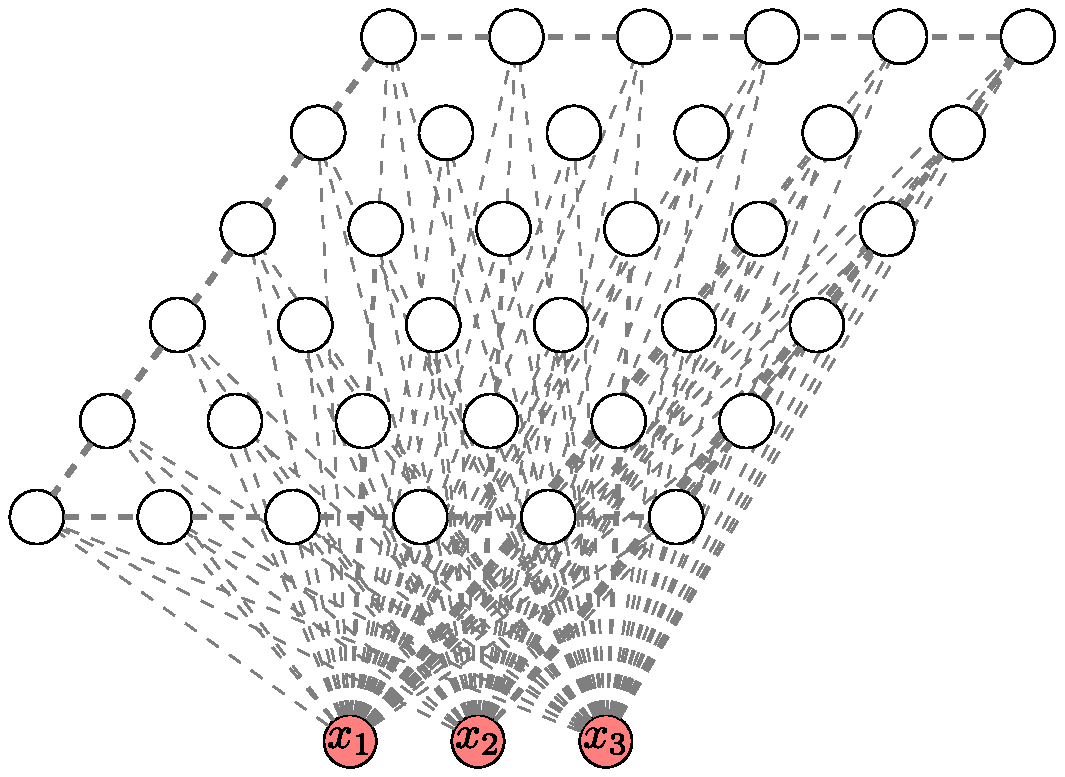
\includegraphics[width=0.75\textwidth]{images/chapter theoritical background/Self-organizing-map.pdf}
  \caption{Η αρχιτεκτονική ενός δισδιάστατου χάρτη αυτο\textendash οργάνωσης που ακολουθεί το μοντέλο του \en{Kohonen}. \textit{Παράχθηκε από το \href{https://inkscape.org/}{\en{Inkscape}} τροποποιώντας \href{https://commons.wikimedia.org/wiki/File:Self-organizing-map.svg}{αυτήν την εικόνα}}.}
  \label{fig:SOM}
\end{figure}

Το μοντέλο \en{Kohonen} που εξετάζουμε ανήκει στην κατηγορία των αλγορίθμων διανυσματικής κωδικοποίησης. Αυτό διότι μέσω του χάρτη \en{Kohonen} παρέχεται μια τοπολογική αντιστοίχηση που τοποθετεί με βέλτιστο τρόπο ένα σταθερό αριθμό διανυσμάτων $w_j, j \in [1, d_x \times d_y]$ σε έναν υψηλότερης διαστατικότητας χώρο δεδομένων εισόδου $S_n, n >> d_x \times d_y$ πραγματοποιώντας κατά αυτόν τον τρόπο συμπίεση δεδομένων με απώλειες \cite{haykin2009neural}. Με απλά λόγια, για κάθε ομάδα από διανύσματα εισόδου που παρουσιαζει τα ίδια μοτίβα ή πρότυπα ($A \subseteq S_n$) αντιστοιχίζεται ένα διάνυσμα $w_j$ που τα περιγράφει (ονομάζεται και κεντροειδές - \en{centroid}). Έτσι, αντί να είναι αποθηκευμένη μια ομάδα από παραπλήσια αλλά διαφορετικά διανύσματα, μπορεί μόνο να αποθηκεύεται το διάνυσμα $w_j$ που τα περιγράφει.

\subsection{Ο Ανθρώπινος Εγκέφαλος ως Πηγή Έμπνευσης}

Έχει παρατηρηθεί ότι ο εγγέφαλος και κυρίως ο εγκεφαλικός φλοιός είναι, σε πολλές περιοχές, οργανωμένος με τρόπο ώστε διαφορετικές αισθητηριακές είσοδοι να αναπαρίσταται από τοπολογικά διατεταγμένους υπολογιστικούς χάρτες\cite{haykin2009neural}. Οι πρώτες ενδείξεις που οδήγησαν σε αυτό το συμπέρασμα ήδη από τον 18ο αιώνα \cite{finger2000minds} οφείλονται στην παρατήρηση ότι τοπικά περιορισμένες εγκεφαλικές κακώσεις προκαλούν συγκεκριμένες παθήσεις \cite{kohonen1990self, eickhoff2018topographic}. Αργότερα, η ιδέα ότι διαφορετικές περιοχές του εγκεφάλου φαίνεται να αφορούν συγκεκριμένες εργασίες αποδείχθηκε με τις σύγχρονες απεικονιστικές μεθόδους \cite{kohonen1990self}. Για παράδειγμα, έχει αποδηχθεί ότι οι απτικές, οι οπτικές και οι ακουστικές αισθητηριακές είσοδοι χαρτογραφούνται  σε διαφορετικές περιοχές του εγκεφαλικού φλοιού με τοπολογικά διατεταγμένο τρόπο\cite{haykin2009neural}.\par

Η διαπίστωση της τοπογραφικής οργάνωσης των λειτουργειών του εγκεφάλου πυροδότησε, όπως θα ήταν αναμενόμενο σε μια εποχή όπου η νευρωεπιστήμη ήταν σε στενή επαφή με την τεχνητή νοημοσύνη, μια σειρά από έρευνες για κατασκευή τεχνητών υπολογιστικών χαρτών. Οι απόπειρες επιδίωκαν να μιμιθούν τους βιολογικούς μηχανισμούς της αυτο\textendash οργάνωσης διατηρώντας τις παρακάτω βασικές αρχές:
\begin{itemize}
  \item Οι νευρώνες πάνω στον υπολογιστικό χάρτη λειτουργούν παράλληλα και επεξεργάζονται ο καθένας πληροφορία εισόδου η οποία προέρχεται από διαφορετικές πηγές (δηλαδή, τα χαρακτηριστικά των διανυσμάτων εισόδου ακολουθούν διαφορετικά πρότυπα).
  \item Σε κάθε χρονική στιγμή, κάθε εισερχόμενη πληροφορία αντιστοιχίζεται στο κατάλληλο νοητικό πλαίσιο (χωρική θέση πάνω στον χάρτη). Με άλλα λόγια, η χωρική θέση ενός νευρώνα εξόδου σε έναν τοπογραφικό χάρτη αντιστοιχεί σε ένα συγκεκριμένο πεδίο (ή πρότυπο) των δεδομένων εισόδου\cite{kohonen1990self}.
  \item Οι νευρώνες που ασχολούνται με στενά σχετιζόμενα πρότυπα εισόδου τοποθετούνται στο πλέγμα κοντά μεταξύ τους (γεγονός που διευκολύνει την συνεργασία).
  \item Ο χάρτης πραγματοποιεί μείωση της διαστατικότητας από τον χώρο των παραμέτρων στον (δισδιάστατο) χώρο αναπαράστασης.\cite{haykin2009neural, knudsen1987computational, durbin1990dimension}
\end{itemize} 
Έχοντας περιγράψει τις βασικές αρχές με τις οποίες οικοδομήθηκαν τα μοντέλα των τεχνητών χαρτών αυτο\textendash οργάνωσης όπως αυτό του \en{Kohonen}, είμαστε σε θέση να περιγράψουμε αναλυτικά τον αλγόριθμο σχηματισμού τους.

\subsection{Αλγόριθμος Σχηματισμού Χάρτη Αυτο\textendash οργάνωσης}

Κάθε αλγόριθμος σχηματισμού χάρτη αυτο\textendash οργάνωσης, για να σέβεται τις τέσσερεις αρχές που παρουσιάστηκαν παραπάνω, πρέπει να πραγματώνει τις εξής τρείς βασικές διαδικασίες:
\begin{enumerate}
  \item Ανταγωνισμού. Σε αυτή τη διαδικασία οι νευρώνες του δικτύου θα πρέπει να ανταγωνίζονται μεταξύ τους για το ποιός είναι ο ποιο κατάλληλος να εξηγήσει το εκάστοτε δείγμα εισόδου. Ο νικητής του ανταγωνισμού για το συγκεκριμένο δείγμα (έστω $x_i$) είναι αυτός με την μεγαλύτερη επίδοση, όπως αυτή υπολογίζεται από μια συνάρτηση διάκρισης.
  \item Συνεργασίας. Σε αυτή, ο νικιτής νευρώνας καθορίζει το εύρος της χωρικής γειτονιάς οι νευρώνες της οποίας θα διεγερθούν ταυτόχρονα με τον νευρώνα νικητή, ενισχύοντας έτσι μια σχέση συνεργασίας\footnote{Η συνεργασία η οποία διαμορφώνεται από την ταυτόχρονη πυροδότηση γειτονικών νευρώνων βασίζεται στην Χεμπιανή μάθηση, όπως την αναφέραμε στην ενότητα \ref{sec:historic_note}}.
  \item  Προσαρμογής Συναπτικών Βαρών. Σε αυτή τη διαδικασία λαμβάνει χώρα η μεταβολή των βαρών $w$ των διεγερμένων νευρώνων σε κατεύθυνση ώστε να αυξάνεται η επίδοσή τους σε σχέση με το πρότυπο που ακολουθεί το δείγμα εισόδου $x_i$ (όπως μετράται από την συνάρτηση διάκρισης).\cite{haykin2009neural}
\end{enumerate}

Στον επαναληπτικό αλγόριθμο για το σχηματισμό χάρτη αυτο\textendash οργάνωσης του \en{Kohonen}, τα βήματα με τα οποία υλοποιούνται οι ανωτέρω διαδικασίες είναι πέντε:
\begin{enumerate}
  \item Αρχικοποίηση. Στο βήμα αυτό αρχικοποιούνται τα βάρη όλων των νευρώνων του πλέγγματος με τυχαίες, μικρές τιμές\footnote{Εναλλακτικά, αρικοποιούνται λαμβάνοντας τυχαία δείγματα από το σύνολο δεδομένων εισόδου $S_n$.}. Θα μπορούσε για παράδειγμα να είναι:
  \begin{equation}
    w_0(0) \sim \mathcal{N}(\boldsymbol{\mu},\boldsymbol{\varSigma}), \boldsymbol{\mu} = \mathcal{O}_{m\times 1} , \boldsymbol{\varSigma} = \mathcal{I}_m, \forall j \in [1, d_x \times d_y].
  \end{equation}

  \item Δειγματοληψία. Σε αυτό το στάδιο λαμβάνεται τυαία ένα δείγμα εισόδου $x_i \in \Re^m$ από το σύνολο δεδομένων $S_n$. Το δείγμα αντιπροσοπεύει το πρότυπο ενεργοποίησης (ερέθισμα) που εφαρμόζεται στο πλέγμα. Εναλλακτικά, τα δείγματα $x_i$ μπορούν να λαμβάνονται σηρειακά από το σύνολο δεδομένων εισόδου.
  
  \item Ταίριασμα Ομοιότητας. Εδώ λαμβάνει χώρα ο ανταγωνισμός μεταύ των νευρώνων. Σε αυτό το βήμα, δοσμένου του προτύπου ενεργοποίησης $x_i$ επιλέγεται ο νευρώνας νικιτής $v(x_i), v(x_i) \in \mathcal{A} $. Η συνάρτηση διάκρισης που χρησιμοποιείται είναι αυτή της ελάχιστης ευκλείδιας απόστασης\footnote{Εναλλακτικά, θα μπορούσε να χρησιμοποιηθεί το συνημίτονο ομοιότητας ως κριτήριο επιλογής του νικητή. Άλλωστε, το κριτήριο βέλτιστης ταύτησης βάση της μεγιστοποίησης του εσωτερικού γινομένου μεταξύ των διανυσμάτων $w_j, \forall j \in [1, d_x \times d_y]$ και $x_i$ (\en{cosine similarity}) είναι μαθηματικώνς ισοδύναμο με το κριτήριο της ελαχιστοποίησης της Ευκλείδιας απόστασης με την προυπόθεση ότι τα διανύσματα βαρών των νευρώνων έχουν μοναδιαίο μήκος\cite{haykin2009neural}.}. Έτσι, με μαθηματικούς όρους, έχουμε:
  \begin{equation}
    v(x_i) = \underset{j}{\mathrm{argmax}} \lVert x_i - w_j \rVert , j \in [1, d_x \times d_y].
  \end{equation}

  \item Ενημέρωση. Σε αυτό το σημείο πραγματοποιούντια οι σημαντικές διαδικασίες της συνεργασίας και της προσαρμογής συναπτικών βαρών. Αναλυτικότερα, τα βάρη των νευρώνων του πλέγματος ανανεώνονται από την παλιά τιμή τους που είχαν την χρονική στιγμή $t$ στην νέα τους τιμή μέσω του τύπου: 
  \begin{equation}
    w_j(t+1) = w_j(t) + \eta(t) h_{j,v(x_i)}(t)(x_i-w_j(t)).
  \end{equation}
  Όπου $\eta(t)$ είναι μια συνάρτηση\textendashυπερπαράμετρος που καθορίζει τον ρυθμό μάθησης ανάλογα με τον αριθμό των επαναλήψεων που έχουν παρέλθει ($t$). Μια κατάλληλη τέτοια συνάρτηση είναι η
  \begin{equation}
    \eta(t) = \eta_0 \exp{-\frac{t}{\tau_2}}
  \end{equation}
  όπου $\tau_2$ μια σταθερά (υπερπαράμετρος) χρόνου και $\eta_0$ μια τιμή ρυθμού μάθησης κετά την εκκίνηση (όταν $t=0$).
  
  $h_{j,v(x_i)}(t)$ είναι η συνάρτηση\textendashυπερπαράμετρος που ορίζει μια γειτονιά ενεργοποιημένων νευρώνων γύρω από τον νευρώνα νικητή. Είναι σημαντικό να τονίσουμε ότι η γειτονιά εαρτάται από την πλευρική απόσταση  (\en{lateral distance}) μεταξύ του νευρώνα νικητή και των υπόλοιπων νευρώνων στο πλέγμα, όπως αυτή υπολογίζεται στον (συνήθως δισδιάστατο) χώρο εξόδου. Δηλαδή, για τον υπολογισμό της γειτνίασης μεταύ δύο νευρώνων, δεν λαμβάνονται υπόψη τα βάρη τους $w$ παρά μόνο η σχετική τους απόσταση $d_{j,v}$ πάνω στο πλέγμα. Μια κατάλληλη επιλογή της συνάρτησης γειτονιάς είναι:
  \begin{equation}
    h_{j,v(x_i)}(t) = exp{-\frac{d^2_{j,v}}{2\sigma^2(t)}}
  \end{equation}
  όπου το $\sigma(t)$ καθορίζει το εύρος της τοπολογικής γειτονιάς και είναι:
  \begin{equation}
    \sigma(t) = \sigma_0 exp{-\frac{t}{\tau_1}}
  \end{equation}
  όπου $\tau_1$ μια σταθερά χρόνου και $\sigma_0$ η τιμή αρχικού εύρους.

  \item Συνέχιση. Το τελευταίο αυτό βήμα εξετάζει αν οι αλλαγές στο χάρτη χαρακτηριστικών είναι ευδιάκριτες. Αν κάτι τέτοιο είναι αληθές, τότε επαναφέρει την ροή προγράμματος στο βήμα 2. Αλλιώς, ο αλγόριθμος έχει συγκλίνει και συνεπώς τερματίζει.
\end{enumerate}

Σαν τελικά σχόλια σχετικά με τον αλγόριθμο σχηματισμού αυτο\textendash οργανούμενου χάρτη να αναφέρουμε ότι βοηθάει αν χωρίσουμε την εκπαίδευση σε δύο φάσεις: την φάση αυτο\textendash οργάνωσης και την φάση σύγκλισης. Στην πρώτη, λαμβάνει χώρα η τοπολογική διάταξη των διανυσμάτων των βαρών και συνήθως τόσο το εύρος της γειτονιάς όσο και ο ρυθμός μάθησης έχουν μεγάλες τιμές (οι οποίες βαθμιαία μειώνονται). Στην δεύτερη φάση, πραγματοποιούνται λεπτές προσαρμογές στον χάρτη έτσι ώστε να παρέχει μια επακριβή στατιστική ποσοτικοποίηση του χώρου εισόδου\cite{haykin2009neural}. Για τον σκοπό αυτό, ευπηρετεί η ανάθεση των υπερπαραμέτρων που καθορίουν το μέγεθος της γειτονιάς και τον ρυθμό μάθησης σε μικρές τιμές.
% \section{Αλγόριθμος \en{EM}}
% \label{sec:_EM}
% \section{Συμπερασματολογία μέσω Διακύμανσης}
% autoencoders
